\documentclass[12pt, a4paper]{report}

% --- Packages ---
\usepackage[utf8]{inputenc}
\usepackage{arabtex}
\usepackage{utf8}
\setcode{utf8}

\usepackage{graphicx}
\usepackage{epstopdf-base} % preload: arabtex begin-document hook otherwise loads it inside a group (TL2026 error)
\usepackage{geometry}
\geometry{a4paper, top=1.5in, bottom=1.5in, left=1in, right=1in}
\usepackage{setspace}
\setstretch{1.2} % Compact body (AAST asks 1.5; tighter for readability vs page count)
\usepackage{mathptmx} % Times New Roman style font
\usepackage{amsmath} % Required for \text{} inside math equations
\usepackage{amssymb} % \mathbb{R} etc. in Ch 3--4 methodology
\usepackage{url} % Bibliography URLs (references.bib)
\usepackage[normalem]{ulem} % Allows underlined text to wrap safely
\usepackage{caption} % AAST §2.4.1 figure/table caption formatting

% Figure captions: 10 pt bold centred; 4 pt above, 10 pt below
\captionsetup[figure]{
  font={bf,footnotesize},
  labelfont=bf,
  textfont=bf,
  justification=centering,
  singlelinecheck=false,
  position=below
}
% Table titles: 12 pt bold centred (all chapters via float hook + width)
\captionsetup[table]{
  font=bf,
  labelfont=bf,
  textfont=bf,
  justification=centering,
  singlelinecheck=true,
  position=above,
  skip=6pt,
  width=\linewidth,
  margin=0pt
}
\setlength{\arrayrulewidth}{0.4pt} % Visible full grid borders in tables
\setlength{\abovecaptionskip}{4pt}
\setlength{\belowcaptionskip}{10pt}

% Acronym list always appears (not only printonlyused)
\usepackage{acronym}

\usepackage{array} % Prevents text stretching and underfull warnings
\renewcommand{\arraystretch}{1.15} % Readable row height in grid tables
\setlength{\tabcolsep}{5pt}
\usepackage{float} % [H] figure placement — keeps figures with their section}
\usepackage{needspace} % \Needspace — avoid orphaned headings and split floats
\usepackage{etoolbox} % hook figure/table environments for keep-together breaks
\newcolumntype{P}[1]{>{\raggedright\arraybackslash}p{#1}} % Wrapping text columns

% Widow/orphan control: discourage single lines stranded at page top/bottom
\widowpenalty=10000
\clubpenalty=10000
\displaywidowpenalty=10000

% Keep floats with their section (use with [H] figures/tables)
\AtBeginEnvironment{figure}{\Needspace{14\baselineskip}}
\AtBeginEnvironment{table}{%
  \Needspace{10\baselineskip}%
  \centering
  \captionsetup{justification=centering, singlelinecheck=true, width=\linewidth}%
}

% Manual \textbf{1.x} headings (no \section): keep title + intro + first subsection
\newenvironment{secopen}{%
  \Needspace{9\baselineskip}%
  \begin{samepage}%
}{%
  \end{samepage}%
}
\newcommand{\secneed}{\Needspace{9\baselineskip}}
\newcommand{\subsecneed}{\Needspace{5\baselineskip}}

% Chapter-prefixed floats (1-1, 2-1, …) — chapters use manual headings, not \chapter{}
\newcommand{\startchapterfloats}[1]{%
  \setcounter{figure}{0}%
  \setcounter{table}{0}%
  \renewcommand{\thefigure}{#1-\arabic{figure}}%
  \renewcommand{\thetable}{#1-\arabic{table}}%
}

% --- Arabic inline helper (RTL snippet inside English LTR text) ---
\newcommand{\arTxt}[1]{\RL{#1}}

% --- TOC/LOF/LOT Layout (AAST: titles left-aligned, all caps) ---
\usepackage{tocloft} % legacy nottoc,notlof,notlot options removed: rejected by TeX Live 2026, never used by tocloft

\renewcommand{\contentsname}{TABLE OF CONTENTS}
\renewcommand{\listfigurename}{LIST OF FIGURES}
\renewcommand{\listtablename}{LIST OF TABLES}

% Left-align list page titles (not centred)
\renewcommand{\cfttoctitlefont}{\Large\bfseries}
\renewcommand{\cftaftertoctitle}{\par\vspace{0.4cm}}
\renewcommand{\cftloftitlefont}{\Large\bfseries}
\renewcommand{\cftafterloftitle}{\par\vspace{0.4cm}}
\renewcommand{\cftlottitlefont}{\Large\bfseries}
\renewcommand{\cftafterlottitle}{\par\vspace{0.4cm}}

% 1. Format Chapter entries (Bold text + Dotted leaders)
\renewcommand{\cftchapfont}{\bfseries}
\renewcommand{\cftchappagefont}{\bfseries}
\renewcommand{\cftchapleader}{\cftdotfill{\cftdotsep}}

% 2. Format Section entries (Bold text + Dotted leaders)
\renewcommand{\cftsecfont}{\bfseries}
\renewcommand{\cftsecpagefont}{\bfseries}
\renewcommand{\cftsecleader}{\cftdotfill{\cftdotsep}}

% 3. Format Subsection entries (Regular text + Dotted leaders)
\renewcommand{\cftsubsecfont}{\normalfont}
\renewcommand{\cftsubsecpagefont}{\normalfont}
\renewcommand{\cftsubsecleader}{\cftdotfill{\cftdotsep}}

% Prevents technical jargon from breaking margins across the whole book
\emergencystretch=1em

\begin{document}

% --- Front Matter ---
\begin{titlepage}
    \centering
    
    % 1. Logo (AAST template: 3.25 cm x 3.25 cm)
    
\includegraphics[width=3.25cm,height=3.25cm,keepaspectratio]{images/aast_logo.png}\par\vspace{0.8cm}
    
    % 2. Academy & College Details
    {\large \textbf{Arab Academy for Science, Technology and Maritime Transport}}\par\vspace{0.6cm}
    {\large \textbf{College of Engineering and Technology}}\par\vspace{0.2cm}
    {\large \textbf{Computer Engineering Department}}\par\vspace{1cm}
    
    % 3. Project Type
    {\large B. Sc. Final Year Project}\par\vspace{1cm}
    
    % 4. Project Title (ALL CAPS per AAST template)
    {\Large \textbf{A BILINGUAL SIGN LANGUAGE RECOGNITION AND COMMUNICATION SYSTEM}}\par\vspace{0.4cm}
    {\large \textbf{Real-Time Letter and Word Recognition with a Web-Based Deployment}}\par\vspace{1.5cm}
    
    % 5. Authors (Students)
    {\large Presented By:}\par\vspace{0.8cm}
    
    \begin{center}
        \large
        % Changed 'l' to 'c' to center the names within their columns
        \begin{tabular}{@{} c @{\hspace{1.2cm}} c @{}}
            \textit{Ahmed Adel Sayed Gouda Ahmed} & \textit{Hadeel Gamal Eldin Mohamed Ibrahim}  \\[0.4cm]
            \textit{Alaa Osama Mohammed Shehab} & \textit{Salah Mohamed Salah Ibrahim} \\
        \end{tabular}
    \end{center}
    \par\vspace{1.3cm}
    
    % 6. Supervisors
    {\large Supervised By:}\par\vspace{0.6cm}
    % Supervisor names are correctly italicized
    {\large \textit{Dr. Nada Mostafa Abdelaziem Mostafa}}\par\vspace{0.3cm}
    {\large \textit{Dr. Reham Taher Abdelmajeed Salem Al Magraby}}\par\vfill
    
    % 7. Date (Changed to \footnotesize to achieve exact 10pt size)
    {\footnotesize July -- 2026}
   
\end{titlepage}

\clearpage
\newpage
\thispagestyle{empty} 

\begin{center}
    \Large \textbf{\uline{DECLARATION}}
\end{center}
\vspace{0.8cm}

\normalsize
\noindent I hereby certify that this report, which I now submit for assessment on the program of study leading to the award of Bachelor of Science in \textit{Computer Engineering}, is all my own work and contains no Plagiarism. By submitting this report, I agree to the following terms:\vspace{0.2cm}

\begin{quote}
    \textit{Any text, diagrams or other material copied from other sources (including, but not limited to, books, journals, and the internet) have been clearly acknowledged and cited followed by the reference number used; either in the text or in a footnote/end-note. The details of the used references that are listed at the end of the report confirm the referencing style dictated by the final year project template and are, to my knowledge, accurate and complete.}
\end{quote}
\vspace{0.2cm}

% THE FIX: \raggedright clears the overfull margin warning completely
\noindent{\raggedright I have read the sections on referencing and plagiarism in the final year project template. \uline{I understand that plagiarism can lead to a reduced or fail grade, in serious cases, for the Graduation Project course.}}\par\vspace{1.2cm}

% --- Signatures Section ---
\noindent
\begin{tabular}{@{} >{\raggedright\arraybackslash}p{0.46\textwidth} >{\raggedright\arraybackslash}p{0.46\textwidth} @{}}
    \textbf{Student Name:} Ahmed Adel Sayed Gouda Ahmed & \textbf{Student Name:} Hadeel Gamal Eldin Mohamed Ibrahim \\[0.3cm]
    \textbf{Registration Number:} 211005618 & \textbf{Registration Number:} 211004219  \\[0.3cm]
    \textbf{Signed:} \rule{4.5cm}{0.4pt} & \textbf{Signed:} \rule{4.5cm}{0.4pt} \\[1cm]
    
    \textbf{Student Name:} Alaa Osama Mohammed Shehab & \textbf{Student Name:} Salah Mohamed Salah Ibrahim \\[0.3cm]
    \textbf{Registration Number:} 211004234 & \textbf{Registration Number:} 211004521 \\[0.3cm]
    \textbf{Signed:} \rule{4.5cm}{0.4pt} & \textbf{Signed:} \rule{4.5cm}{0.4pt} \\
\end{tabular}

\vfill 

\noindent \textbf{Date:} Wednesday 8\textsuperscript{th} June 2026
\newpage
\thispagestyle{plain} 

\begin{center}
    \Large \textbf{ACKNOWLEDGMENTS}
\end{center}
\vspace{0.8cm}

\normalsize
\noindent In the name of Allah, the Most Gracious, the Most Merciful, to whom we attribute the strength and success to complete this research.\par\vspace{0.4cm}

We are profoundly grateful to our supervisor, \textbf{Dr. Nada Mostafa Abdelaziem Mostafa}, for her unwavering patience, invaluable expertise, and continuous guidance. Her insights not only shaped the technical direction of this thesis but have also deeply enriched our broader understanding of computer engineering and intelligent systems.\par\vspace{0.4cm}

Equally, we owe our deepest appreciation to \textbf{Dr. Reham Taher Abdelmajeed Salem Al Magraby}. Her transformative support, constant motivation, and words of wisdom were the driving force behind this project. Without her dedicated mentorship and encouragement, the realization of this work would not have been possible. Truly, she has taught us a great deal, and for that, we are immensely grateful.\par\vspace{0.4cm}

We consider ourselves truly fortunate to have worked under the supervision of such exceptional educators, and we hope this thesis serves as a worthy testament to their efforts and guidance.\par\vspace{0.4cm}

Furthermore, we would like to extend our collective and heartfelt thanks to our parents and families for never failing to encourage us to be the best versions of ourselves. Their endless sacrifices and their efforts in instilling the value of hard work and the importance of knowledge within us have been our greatest foundation.\par\vspace{0.4cm}

Finally, a special note of gratitude to all our siblings and loved ones. Without your constant support and encouragement, we would have never been able to accomplish our goals and bring this project to life.
\newpage
\thispagestyle{plain} 

\begin{center}
    \Large \textbf{ABSTRACT}
\end{center}
\vspace{0.8cm}

\normalsize

\noindent Sign language recognition systems can reduce communication barriers between deaf and hard-of-hearing communities and hearing users, yet most practical tools cover only one language or one recognition level. This graduation project delivers \textbf{Eshara} (\arTxt{إشارة}), a bilingual \textbf{web application} for American Sign Language (ASL) and Arabic Sign Language (ArSL) that supports static letter finger-spelling and isolated-word recognition from a standard webcam.\par\vspace{0.45cm}

\noindent The system follows a three-tier architecture: a \textbf{React} frontend, a \textbf{Node.js/Express} application layer for authentication and routing, and a \textbf{FastAPI} model-services layer for inference. Four standalone deep-learning models are trained with separate vocabularies: an ASL letter \textbf{MLP} over \textbf{78-D} engineered hand landmarks (\textbf{28} deployed classes), an ArSL letter \textbf{MLP} over \textbf{63-D} raw hand landmarks (32 classes), an ASL word \textbf{Inception I3D} model over \textbf{32-frame} \textbf{224$\times$224} RGB clips (100 WLASL glosses), and an ArSL word stacked \textbf{BiLSTM} over \textbf{225-D} normalised Holistic sequences (48 frames, 100 KArSL classes).\par\vspace{0.45cm}

\noindent Under constrained compute and single-academic-year scope, verification combines held-out dataset evaluation, integration testing of the three-tier web stack, and browser latency measurement. Design constraints include limited GPU resources and compact landmark transmission instead of full video streams. ASL and ArSL letters and ASL words are active via \texttt{/predict}; ArSL words are offline-validated and pending web integration. Intended uses include assistive education and communication practice where only a browser and webcam are available.\par


% --- Automatic Indexes (Lowercase Roman Page Numbering: i, ii, iii) ---
\newpage
\pagenumbering{roman}
% ==========================================
%         TABLE OF CONTENTS PAGE
% ==========================================
\thispagestyle{plain}
\tableofcontents
\newpage

% ==========================================
%           LIST OF FIGURES PAGE
% ==========================================
\thispagestyle{plain}
\addcontentsline{toc}{chapter}{\textbf{LIST OF FIGURES}}
\listoffigures
\newpage

% ==========================================
%            LIST OF TABLES PAGE
% ==========================================
\thispagestyle{plain}
\addcontentsline{toc}{chapter}{\textbf{LIST OF TABLES}}
\listoftables
\newpage

% ==========================================
%       LIST OF ACRONYMS/ABBREVIATIONS
% ==========================================
\thispagestyle{plain}
\addcontentsline{toc}{chapter}{\textbf{LIST OF ACRONYMS/ABBREVIATIONS}}

\begin{center}
    {\Large \textbf{LIST OF ACRONYMS/ABBREVIATIONS}}
\end{center}
\vspace{0.8cm}

\begin{table}[H]
\centering
\renewcommand{\arraystretch}{1.5} % Adds vertical padding for readability
\begin{tabular}{|l|l|}
\hline
\textbf{ACRONYM} & \textbf{Definition of Acronym} \\ \hline
\textbf{API} & Application Programming Interface \\ \hline
\textbf{ArSL} & Arabic Sign Language \\ \hline
\textbf{ASL} & American Sign Language \\ \hline
\textbf{BiLSTM} & Bidirectional Long Short-Term Memory \\ \hline
\textbf{CNN} & Convolutional Neural Network \\ \hline
\textbf{CSLR} & Continuous Sign Language Recognition \\ \hline
\textbf{FPS} & Frames Per Second \\ \hline
\textbf{GPU} & Graphics Processing Unit \\ \hline
\textbf{I3D} & Inflated 3D ConvNet \\ \hline
\textbf{JWT} & JSON Web Token \\ \hline
\textbf{KArSL} & King Saud University Arabic Sign Language dataset \\ \hline
\textbf{MLP} & Multilayer Perceptron \\ \hline
\textbf{REST} & Representational State Transfer \\ \hline
\textbf{RTL} & Right-to-Left \\ \hline
\textbf{SLR} & Sign Language Recognition \\ \hline
\textbf{SUS} & System Usability Scale \\ \hline
\textbf{UI} & User Interface \\ \hline
\textbf{WLASL} & Word-Level American Sign Language \\ \hline
\end{tabular}
\end{table}

% --- Main Body (Arabic Page Numbering Starts Here) ---
\newpage
\pagenumbering{arabic}
% ==========================================
%               CHAPTER ONE
% ==========================================
\thispagestyle{plain}

\begin{center}
    \vspace*{0.5cm}
    {\large \textit{Chapter One}} \\[0.4cm]
    {\Large \textbf{1 \quad INTRODUCTION}}
\end{center}
\addcontentsline{toc}{chapter}{\textbf{1 \quad INTRODUCTION}}
\vspace{1in}

\normalsize
\startchapterfloats{1}

% --- 1.1 PROJECT OVERVIEW ---
\noindent\textbf{1.1\quad PROJECT OVERVIEW}\par
\addcontentsline{toc}{section}{\numberline{1.1}PROJECT OVERVIEW}
\vspace{0.4cm}

\noindent This graduation project presents \textbf{Eshara} (\arTxt{إشارة} --- Arabic for ``sign''), a real-time bilingual sign-language recognition system that translates hand gestures from a standard webcam into text through a web application. The system supports American Sign Language (ASL) and Arabic Sign Language (ArSL) at two recognition levels: static letters (finger-spelling) and isolated words signed across a one-to-two second window.\par\vspace{0.4cm}

\noindent Eshara is built as a full-stack web product rather than a laboratory prototype alone. Four deep-learning models --- two Multi-Layer Perceptrons for letter recognition, an Inception I3D network for ASL word recognition, and a BiLSTM for ArSL word recognition --- are designed for a unified web inference pipeline. The deployed stack follows a three-tier path (React client $\rightarrow$ Node.js/Express API $\rightarrow$ FastAPI model-services), with webcam frames captured in the browser, authenticated at the Node layer, and forwarded internally for inference. Input comes from a standard webcam only --- no additional sensors or specialised capture equipment. Letter and ArSL word paths use compact landmark representations (\textbf{78-D} engineered features for ASL letters, \textbf{63-D} raw hand landmarks for ArSL letters, \textbf{225-D} normalised pose-and-hands sequences per frame for ArSL words). The ASL word model operates on \textbf{32-frame} clips of centre-cropped \textbf{224$\times$224} RGB video.\par\vspace{0.4cm}

\noindent The four models are: (1)~an ASL letter MLP over \textbf{28 deployed classes} (78-D input; the source ASL Alphabet corpus contains 29 labels including \texttt{nothing}, which is excluded from the web vocabulary), (2)~an ArSL letter MLP over 32 classes (63-D input), (3)~an ASL word Inception I3D over 100 WLASL glosses, and (4)~an ArSL word BiLSTM over 100 Arabic sign classes (225-D $\times$ 48 frames). Each model was trained and evaluated with Top-1, Top-5, and macro-F1 metrics where applicable. Word methodology is in Chapter~4; experimental results in Chapter~6; full web implementation is in Chapter~5.\par\vspace{0.6cm}

% --- 1.2 PROBLEM STATEMENT ---
\noindent\textbf{1.2\quad PROBLEM STATEMENT}\par
\addcontentsline{toc}{section}{\numberline{1.2}PROBLEM STATEMENT}
\vspace{0.4cm}

\noindent Approximately 466 million people worldwide live with disabling hearing loss, including around seven million in the Arab region~\cite{who2024hearing}. For most deaf and hard-of-hearing individuals, sign language --- not spoken language --- is the primary means of communication. Human sign-language interpreters are effective but costly, limited in availability, and cannot be present in every classroom, clinic, or customer-service interaction. Automated recognition offers a scalable alternative, yet most existing tools and research efforts focus on American Sign Language alone, or on letter recognition alone, and rarely combine both languages and both recognition levels in a single deployable web-based product~\cite{rastgoo2021survey,adaloglou2022comprehensive}.\par\vspace{0.4cm}

\noindent The engineering problem addressed in this thesis is stated formally as follows:\par\vspace{0.3cm}

\begin{quote}
\noindent\textit{Given a continuous RGB video stream from a single uncalibrated camera, automatically recognise either (a)~the letter being finger-spelled per frame, or (b)~the isolated word being signed across a 1--2 second window, in either ASL or ArSL, with end-to-end latency below 200~ms, delivered through a standard web browser.}
\end{quote}
\vspace{0.3cm}

\noindent\textbf{1.2.1\quad Current Constraints:}\par
\addcontentsline{toc}{subsection}{\numberline{1.2.1}Current Constraints:}
\vspace{0.3cm}

\noindent The project was carried out under several practical limits. Training deep recognition models proved time-consuming: feature extraction over tens of thousands of images or video clips required multi-hour (often overnight) CPU/GPU runs, and several model families were trained \textbf{multiple times} after failed webcam trials exposed domain gaps (lighting, background clutter, MediaPipe dropout). The available local GPU (4\,GB VRAM) restricted batch size and forced word-model extraction and I3D experiments onto Kaggle when CUDA memory was exhausted. The full system had to be designed, trained, and evaluated within a single academic year. The solution was required to run in a standard web browser using only a laptop or desktop webcam. For privacy on letter and ArSL word paths, only numeric landmark vectors are sent over the network rather than continuous raw video; ASL word mode instead transmits encoded frame buffers to the server for I3D inference. Software versions and CUDA usage are tabulated as defined in Table~\ref{tab:ch3-env} (Chapter~3).\par\vspace{0.4cm}

\noindent\textbf{1.2.2\quad Technical and Practical Gap:}\par
\addcontentsline{toc}{subsection}{\numberline{1.2.2}Technical and Practical Gap:}
\vspace{0.3cm}

\noindent Several technical and practical gaps motivated this work. Most existing approaches handle either letter recognition or word recognition, but not both within one real-time pipeline. Few systems support more than one sign language in the same product, and many published solutions stop at offline accuracy without a live web interface. Running recognition in the browser is also demanding: inference must stay fast enough for interactive use, yet deep sequence and video models are costly to train and tune under limited compute. Human interpretation remains the default in practice because scalable, low-latency assistive tools are still uncommon. Eshara was designed to address these gaps through a bilingual, dual-level web application accessible from any modern browser.\par\vspace{0.6cm}

% --- 1.3 PROJECT MOTIVE ---
\noindent\textbf{1.3\quad PROJECT MOTIVE}\par
\addcontentsline{toc}{section}{\numberline{1.3}PROJECT MOTIVE}
\vspace{0.4cm}

\noindent The primary motive of this project is to reduce the communication barrier between deaf signers and hearing non-signers in the Arab region and beyond. Arabic sign-language users currently lack the same assistive tooling available to ASL communities. Beyond the social impact, the project demonstrates that specialised models matched to each task --- compact MLPs for letters, a landmark BiLSTM for ArSL words, and a pretrained 3D convolutional network for ASL words --- can achieve strong accuracy within a deployable web application. The final deliverable is intended as a working web product suitable for education, healthcare, customer service, and everyday communication, not merely as an offline accuracy benchmark. The four-model design reflects a deliberate engineering choice: ASL and ArSL have entirely separate vocabularies and feature spaces, so four specialised pipelines --- each tuned to its own input representation and label set --- prove more tractable and more accurate than a single shared multilingual model behind one web interface.\par\vspace{0.6cm}

% --- 1.4 AIMS AND OBJECTIVES ---
\noindent\textbf{1.4\quad AIMS AND OBJECTIVES}\par
\addcontentsline{toc}{section}{\numberline{1.4}AIMS AND OBJECTIVES}
\vspace{0.4cm}

\noindent\textbf{1.4.1\quad Aims:}\par
\addcontentsline{toc}{subsection}{\numberline{1.4.1}Aims:}
\vspace{0.3cm}

\noindent The aim of this project is to design, train, evaluate, and deploy a real-time bilingual ASL/ArSL recognition system that covers both letter and word recognition and is accessible through a web application.\par\vspace{0.4cm}

\noindent\textbf{1.4.2\quad Objectives:}\par
\addcontentsline{toc}{subsection}{\numberline{1.4.2}Objectives:}
\vspace{0.3cm}

\noindent To achieve this aim, six specific objectives were defined. First, four model pipelines were built covering ASL letters, ArSL letters, ASL words, and ArSL words. Second, features were prepared per model: MediaPipe Hand landmarks for letters (\textbf{78-D} engineered for ASL, \textbf{63-D} raw for ArSL), a \textbf{32-frame} RGB clip pipeline for ASL words (I3D), and \textbf{225-D} normalised pose-and-hands sequences over 48 frames for ArSL words. Third, four deep-learning models were trained or integrated: an ASL letter MLP (28 deployed classes), an ArSL letter MLP (32 classes), an ASL word Inception I3D (100 WLASL classes), and an ArSL word BiLSTM (100 classes). Fourth, a three-tier backend path was implemented (Node.js/Express gateway with internal FastAPI model services). Fifth, a React web client was built with a live recognition interface and authenticated translation flow. Sixth, each model was evaluated using Top-1 accuracy, Top-5 accuracy, and macro-F1 on held-out test data; end-to-end latency was measured in the React web application (Chapter~5, Section~5.12).\par\vspace{0.4cm}

\noindent The system deliberately excludes continuous sign-language translation, grammatical parsing, sign languages other than ASL and ArSL, multi-signer scene analysis, native mobile applications, and native depth-camera hardware. These areas are identified as future work in Chapter~9.\par\vspace{0.6cm}

% --- 1.5 LITERATURE REVIEW ---
\begin{secopen}
\noindent\textbf{1.5\quad LITERATURE REVIEW}\par
\addcontentsline{toc}{section}{\numberline{1.5}LITERATURE REVIEW}
\vspace{0.4cm}

\noindent\textit{The following is a summary of the field. A full literature review is presented in Chapter~2.}\par\vspace{0.4cm}

\noindent\textbf{1.5.1\quad Existing Work:}\par
\addcontentsline{toc}{subsection}{\numberline{1.5.1}Existing Work:}
\vspace{0.3cm}

\noindent Sign-language recognition has progressed from early RGB-camera and Hidden Markov Model approaches to deep convolutional and recurrent networks, and more recently to webcam-based landmark pipelines using tools such as MediaPipe~\cite{zhang2020mediapipe,mediapipeweb,rastgoo2021survey}. This project trains or integrates four models aligned to four recognition tasks: ASL letters (28 deployed classes from a 29-label corpus), ArSL letters (32 classes), ASL words (100 WLASL classes via I3D)~\cite{li2020wlasl}, and ArSL words (100 classes)~\cite{sidig2021karsl}. Prior published systems often address only one of these tasks or one language at a time, and rarely deliver all four through a single live web application.\par
\end{secopen}
\vspace{0.4cm}

\noindent\textbf{1.5.2\quad Scholarly Views:}\par
\addcontentsline{toc}{subsection}{\numberline{1.5.2}Scholarly Views:}
\vspace{0.3cm}

\noindent Researchers broadly agree that skeleton and landmark representations require less training data than raw-pixel approaches for many SLR tasks, that 3D convolutional networks capture spatio-temporal motion effectively from video clips, and that sequence models such as BiLSTMs and related temporal encoders outperform per-frame classifiers for landmark-based word recognition. Browser-based deployment is widely recognised as important for practical assistive technology, yet a unified bilingual web product covering letters and words in both ASL and ArSL remains uncommon in the literature.\par\vspace{0.4cm}

\noindent\textbf{1.5.3\quad Challenges and Gaps:}\par
\addcontentsline{toc}{subsection}{\numberline{1.5.3}Challenges and Gaps:}
\vspace{0.3cm}

\noindent Several persistent challenges motivate this project. Letter models must respond per frame with low latency, while word models must capture motion across a short temporal window --- serving both from one web pipeline is non-trivial. Bilingual coverage (ASL and ArSL) and dual granularity (letters and words) multiply the engineering and training effort because each of the four models requires its own architecture and evaluation. Real-time performance demands sustained inference on consumer hardware inside a web browser. Most academic contributions stop at offline accuracy for a single model rather than a unified, deployable four-model web system.\par\vspace{0.4cm}

\noindent\textbf{1.5.4\quad Hypothesis:}\par
\addcontentsline{toc}{subsection}{\numberline{1.5.4}Hypothesis:}
\vspace{0.3cm}

\noindent The central hypothesis of this work is that a webcam-driven pipeline with four specialised deep-learning models --- one per language and recognition level --- deployed in a unified web application can achieve reliable recognition accuracy across all four tasks and end-to-end inference latency of no more than 200~ms in a standard browser. On held-out test data, the letter models reach \textbf{99.06\,\%} (ASL) and \textbf{99.63\,\%} (ArSL) Top-1 accuracy; the ArSL word model reaches \textbf{99.62\,\%} Top-1 on 100 classes; the ASL word I3D checkpoint reaches \textbf{65.89\,\%} Top-1 on the WLASL-100 benchmark (Chapter~6). Full experimental detail for all four models appears in Chapter~6.\par\vspace{0.6cm}

% --- 1.6 METHODOLOGY ---
\begin{secopen}
\noindent\textbf{1.6\quad METHODOLOGY}\par
\addcontentsline{toc}{section}{\numberline{1.6}METHODOLOGY}
\vspace{0.4cm}

\noindent\textit{The following is a high-level overview. Full methodological detail is presented in Chapters~3~(letters) and~4~(words).}\par\vspace{0.4cm}
\clearpage
\noindent\textbf{1.6.1\quad Data Acquisition:}\par
\addcontentsline{toc}{subsection}{\numberline{1.6.1}Data Acquisition:}
\vspace{0.3cm}

\noindent Four datasets underpin the four models. \textbf{Letters:} the Kaggle ASL Alphabet corpus ($\sim$87\,000 images, 29 classes)~\cite{akash2019aslalphabet} and ArASL2018 (54\,049 images, 32 classes)~\cite{arthur2018arasl2018} were converted offline to MediaPipe Hand landmarks; ASL samples use 78-D engineered vectors and ArSL samples use 63-D raw vectors (Chapter~3). \textbf{Words:} ASL word recognition uses a 100-class WLASL subset with 32-frame RGB clips for I3D inference~\cite{li2020wlasl}; ArSL words use the KArSL 100-class word subset (SignID 71--170; 48-frame, 225-D pose-and-hands clips) as described in Chapter~4~\cite{sidig2021karsl}. Extracted letter features and ArSL word sequences are cached as compressed NumPy archives. Letter models use stratified train/validation/test splits; the ArSL word model is evaluated on held-out KArSL clips (SignID 71--170). Trained checkpoints are exported for the web inference service (Chapter~5).\par
\end{secopen}
\vspace{0.4cm}

\noindent\textbf{1.6.2\quad Cleaning and Preprocessing:}\par
\addcontentsline{toc}{subsection}{\numberline{1.6.2}Cleaning and Preprocessing:}
\vspace{0.3cm}

\noindent For \textbf{letters}, static images or live frames pass through MediaPipe Hands; ASL applies wrist-relative normalisation and 15 joint angles before MLP input; ArSL uses raw 63-D coordinates. For \textbf{ASL words}, webcam frames are resized, centre-cropped to 224$\times$224, and normalised to $[-1, 1]$ before buffering 32 frames for I3D input. For \textbf{ArSL words}, Holistic landmarks are nose- and wrist-normalised to a 225-D body-relative representation per frame, then each clip is trimmed or padded to 48 frames (Chapter~4). Clips with missing labels or failed extraction are discarded.\par\vspace{0.4cm}

\noindent Four models were trained or integrated on the processed data. The ASL letter model is a three-hidden-layer MLP (256$\rightarrow$128$\rightarrow$64$\rightarrow$28 softmax) over 78-D input (A--Z, \texttt{space}, \texttt{del}; \texttt{nothing} excluded from deployment). The ArSL letter model uses the same \textbf{MLP family} but a wider head (512$\rightarrow$256$\rightarrow$64$\rightarrow$32 softmax) over 63-D raw input (as compared in Table~\ref{tab:ch3-arch-compare}, Chapter~3). The ASL word model is a pretrained \textbf{Inception I3D} (Inflated 3D ConvNet) with a 100-way WLASL classification head. The ArSL word model is a stacked BiLSTM network over 225-D $\times$ 48 frames and 100 classes. The full three-tier deployment is described in Chapter~5.\par\vspace{0.6cm}

% --- 1.7 REPORT ORGANISATION ---
\secneed
\noindent\textbf{1.7\quad REPORT ORGANISATION}\par
\addcontentsline{toc}{section}{\numberline{1.7}REPORT ORGANISATION}
\vspace{0.4cm}

\noindent The remainder of this report is organised as follows. Chapter~2 presents the literature review, tracing sign-language recognition from early Hidden Markov Model and RGB-camera systems through deep convolutional and recurrent networks to modern hybrid landmark- and video-based pipelines, and identifying the gap that motivates this work. Chapter~3 details the letter-recognition methodology for both ASL and ArSL, covering dataset preparation, landmark feature engineering, MLP architecture, and training protocol. Chapter~4 presents the word-recognition methodology: the Inception I3D pipeline for ASL words and the BiLSTM pipeline for ArSL words, including feature extraction and model-side inference protocols.\par\vspace{0.3cm}

\subsecneed
\noindent Chapter~5 describes the full system implementation --- React frontend, Node.js/Express application tier, FastAPI model-services tier, live web recognition interface, and real-time latency measurements. Chapter~6 reports experimental results for all four models, including Top-1 and Top-5 accuracy, macro-F1, and ablation evidence. Chapter~7 discusses and interprets those results in the context of prior work, limitations, and the project hypothesis. Chapter~8 states the conclusions. Chapter~9 identifies directions for future work including continuous sign translation, extended vocabulary, and multilingual expansion.\par

\newpage
% ==========================================
%               CHAPTER TWO
% ==========================================
\thispagestyle{plain}

\begin{center}
    \vspace*{0.5cm}
    {\large \textit{Chapter Two}} \\[0.4cm]
    {\Large \textbf{2 \quad LITERATURE REVIEW}}
\end{center}
\addcontentsline{toc}{chapter}{\textbf{2 \quad LITERATURE REVIEW}}
\vspace{0.45in}

\normalsize
\startchapterfloats{2}

\noindent Chapter~1 stated the problem, objectives, and scope of Eshara: a \textbf{web-only}, webcam-driven bilingual sign-language system with four standalone recognition models. This chapter reviews the literature that motivates those design choices. The review proceeds in a deliberate funnel: technological history of SLR (Section~2.1); machine-learning foundations (Section~2.2); computer-vision input representations (Section~2.3); deep-learning architectures (Section~2.4); pose-estimation frameworks (Section~2.5); datasets (Section~2.6); bilingual and Arabic research (Section~2.7); real-time web deployment (Section~2.8); the research gap Eshara addresses (Section~2.9); and a consolidated comparison of the four graduation models (Section~2.10). Chapters~3 and~4 implement the protocols justified here; Chapter~6 reports offline accuracy and Chapter~5 reports live web performance.\par\vspace{0.3cm}

% --- 2.1 HISTORY ---
\noindent\textbf{2.1\quad HISTORY OF SIGN-LANGUAGE RECOGNITION}\par
\addcontentsline{toc}{section}{\numberline{2.1}HISTORY OF SIGN-LANGUAGE RECOGNITION}
\vspace{0.2cm}

\noindent Three terms recur throughout this thesis and the SLR literature. \textbf{Sign-language recognition (SLR)} maps signing video or pose features to discrete \textbf{gloss} labels (individual signs). \textbf{Sign-language translation (SLT)} maps entire signing utterances to spoken-language sentences, often without an explicit gloss intermediate~\cite{camgoz2018neural}. \textbf{Isolated} SLR classifies one sign per clip; \textbf{continuous} SLR or CSLR decodes unsegmented video into gloss sequences~\cite{koller2020weakly,duarte2021how2sign}. Eshara implements isolated SLR only: the user deliberately signs one letter or one word at a time. Continuous translation is acknowledged as future work in Chapter~9.\par\vspace{0.2cm}

\noindent Sign-language recognition (SLR) has evolved through three broad technological phases, each driven by hardware availability and the maturation of machine-learning methods~\cite{rastgoo2021survey,sterpu2018sign,adaloglou2022comprehensive}. In the 1990s and early 2000s, researchers relied on instrumented gloves, accelerometers, and magnetic trackers that measured joint angles directly. Starner et al.\ demonstrated real-time American Sign Language recognition from wearable and desk-mounted cameras paired with specialised sensing equipment~\cite{starner1998realtime}. These approaches achieved usable accuracy in controlled settings but required expensive hardware and were unsuitable for everyday communication by deaf and hard-of-hearing users, who number in the hundreds of millions worldwide~\cite{who2024hearing}. The fundamental lesson from this era is that high-quality sensing does not guarantee deployability: assistive tools must work with hardware users already own.\par\vspace{0.2cm}

\noindent From the mid-2000s onward, commodity RGB cameras enabled vision-based systems that tracked hand shape and motion without worn sensors. Hidden Markov Models (HMMs) treated signing as a sequence of discrete visual states and remained the dominant statistical framework for more than a decade~\cite{rabiner1989tutorial,koller2015continuous,koller2016continuous}. HMMs are effective when hand segmentation is reliable and vocabularies are small, but they struggle with high intra-class variation in unconstrained webcam video. The introduction of depth cameras such as Microsoft Kinect around 2010 enabled skeleton joints to be recovered without gloves; however, depth hardware never achieved universal adoption in laptops and phones, limiting long-term impact for consumer-facing assistive products~\cite{rastgoo2021survey}.\par\vspace{0.2cm}

\noindent Convolutional neural networks (CNNs) later replaced hand-crafted features for many SLR pipelines, learning spatial filters directly from pixels or optical-flow stacks~\cite{he2016deep,koller2016continuous,pigou2018sign}. CNN-based isolated sign classifiers routinely exceed 90\,\% accuracy on curated benchmarks, yet still exhibit sensitivity to background clutter, lighting variation, signer skin tone, and camera resolution. Koller et al.\ advanced \emph{continuous} sign recognition through hybrid CNN--HMM architectures trained on broadcast footage, establishing a research line that later extended to weakly supervised sequence learning when frame-level gloss labels are incomplete~\cite{koller2020weakly}. This distinction between \emph{isolated} sign classification (one sign per clip) and \emph{continuous} recognition (unsegmented sentences) is central to Eshara: the graduation system solves isolated letter and word recognition; sentence-level gloss alignment is deferred to future work~\cite{duarte2021how2sign,forster2014rwth}.\par\vspace{0.2cm}

\noindent A third phase began with robust single-camera pose estimation. OpenPose demonstrated that body keypoints could be recovered in real time from monocular video~\cite{cao2019openpose}, and Google's MediaPipe extended this to efficient hand and body landmark extraction on consumer hardware~\cite{zhang2020mediapipe,bazarevsky2020blazepose}. Recent sign-language systems increasingly operate on skeleton or landmark feature vectors rather than raw pixels, reducing data requirements and enabling browser-side extraction~\cite{adaloglou2022comprehensive}. Parallel research on continuous sign-language recognition and sign-language translation treats entire sentences as sequences of glosses, typically using hybrid convolutional-recurrent or transformer encoders~\cite{camgoz2018neural,duarte2021how2sign}. The present project, Eshara, sits in a \textbf{hybrid isolated-sign paradigm}: letters and ArSL words use MediaPipe landmarks; ASL words use buffered RGB clips. The system recognises individual letters and short isolated word signs from a standard webcam, and leaves full continuous translation to Chapter~9.\par\vspace{0.2cm}

\begin{figure}[H]
\centering
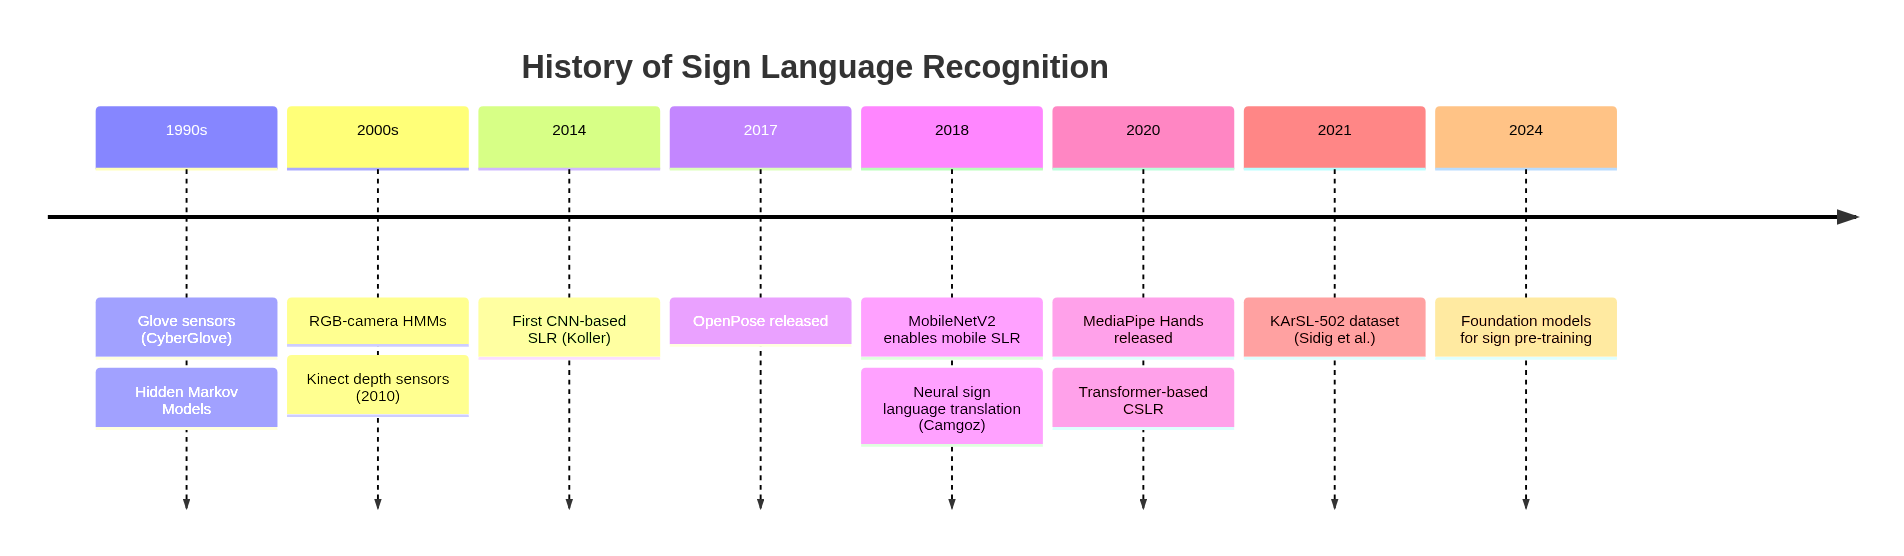
\includegraphics[width=0.92\textwidth]{images/fig_2-1_slr_timeline.png}
\caption{Evolution of sign-language recognition from sensor gloves and HMM-based RGB pipelines to landmark-based deep learning on commodity webcams.}
\label{fig:slr-timeline}
\end{figure}
\vspace{0.2cm}

\noindent As summarised in Figure~\ref{fig:slr-timeline}, the timeline captures the milestones above. The following table interprets the timeline in terms of \emph{what the system measures}, \emph{what model family dominated}, and \emph{whether ordinary users could deploy it} --- three questions that directly motivated Eshara's design.\par\vspace{0.2cm}

\begin{table}[H]
\centering
\caption{Interpretation of SLR technological eras (aligned with Figure~\ref{fig:slr-timeline}).}
\label{tab:slr-eras}
\small
\begin{tabular}{|P{1.35cm}|P{2.55cm}|P{2.35cm}|P{1.75cm}|P{2.9cm}|}
\hline
\multicolumn{1}{|c|}{\textbf{Period}} & \multicolumn{1}{|c|}{\textbf{Input to classifier}} & \multicolumn{1}{|c|}{\textbf{Dominant models}} & \multicolumn{1}{|c|}{\textbf{Deployability}} & \multicolumn{1}{|c|}{\textbf{Relevance to Eshara}}\\
\hline
1990s & Glove joint angles & HMM, template matching & Low (wearable hardware) & Historical only \\
\hline
2000s--2010 & RGB pixels, depth maps & HMM, early CNN & Medium (lab cameras) & Motivated vision path \\
\hline
2014--2017 & CNN features from video & CNN, CNN+HMM & Medium--high & Informed CNN trials \\
\hline
2017--2020 & Body/hand keypoints & CNN+RNN, attention & Rising & OpenPose/MediaPipe era \\
\hline
2020--2024 & Landmark vectors & BiLSTM, Transformer & \textbf{High} (webcam + browser) & \textbf{Eshara's era} \\
\hline
\end{tabular}
\end{table}
\vspace{0.2cm}

\noindent\textbf{Reading the timeline milestone by milestone.} In the \textbf{1990s}, CyberGlove-style sensors proved that sign patterns could be recognised automatically, but users had to wear equipment. Researchers therefore sought camera-only solutions. Through the \textbf{2000s}, standard webcams and HMMs allowed finger-spelling experiments without gloves; accuracy was acceptable when backgrounds were controlled, but models did not generalise to casual home environments~\cite{koller2015continuous}. \textbf{Kinect (2010)} added depth maps and skeleton joints without gloves, yet depth cameras were not built into most laptops, so the approach did not become a universal assistive platform~\cite{rastgoo2021survey}.\par\vspace{0.2cm}

\noindent \textbf{2014} marks wider adoption of CNNs for hand-shape recognition (Koller et al.) --- networks learn their own visual features instead of hand-crafted descriptors~\cite{koller2016continuous}. \textbf{2017} brought OpenPose, showing that 2-D body pose could be recovered from a single RGB stream in real time~\cite{cao2019openpose}. \textbf{2018} added two parallel threads: efficient CNNs such as MobileNetV2 for resource-constrained devices~\cite{sandler2018mobilenetv2}, and neural sign-language translation systems that map entire signing sequences to spoken-language sentences~\cite{camgoz2018neural}. \textbf{2020} is a turning point for deployable SLR: MediaPipe Hands made robust hand tracking available on consumer hardware and in the browser~\cite{zhang2020mediapipe,mediapipeweb}, while transformer-based models advanced continuous sign recognition on large corpora~\cite{vaswani2017attention,koller2020weakly}.\par\vspace{0.2cm}

\noindent \textbf{2021} saw the release of KArSL-502, the first large-scale Arabic sign-language video benchmark used in this thesis~\cite{sidig2021karsl}. \textbf{2024} research explores foundation-model pre-training on massive video corpora; such models are promising but require compute and data beyond graduation scope~\cite{adaloglou2022comprehensive}. Eshara deliberately occupies the \textbf{2020--2024 deployable-webcam band}: a webcam feeds MediaPipe landmarks for letters and ArSL words, or buffered RGB clips for ASL words; lightweight supervised classifiers (MLP, BiLSTM, or I3D) map inputs to text; the user signs \emph{one isolated letter or word at a time}. Continuous sentence recognition (How2Sign, RWTH-PHOENIX) is acknowledged in the literature but deferred to Chapter~9~\cite{duarte2021how2sign,forster2014rwth}.\par\vspace{0.3cm}

% --- 2.2 MACHINE LEARNING FOUNDATIONS ---
\noindent\textbf{2.2\quad MACHINE LEARNING FOUNDATIONS FOR SLR}\par
\addcontentsline{toc}{section}{\numberline{2.2}MACHINE LEARNING FOUNDATIONS FOR SLR}
\vspace{0.2cm}

\noindent This section introduces the machine-learning concepts used throughout Eshara so that readers without a deep-learning background can follow Chapters~3--5. Notation is kept light: formal equations, tensor dimensions, and training objectives appear in Chapter~3 (letter models) and Chapter~4 (word models). Sign-language recognition in this project is cast entirely as \textbf{supervised learning}: the system learns from labelled examples (images or videos with known sign classes) and predicts a class label for new inputs at inference time~\cite{rastgoo2021survey}.\par\vspace{0.2cm}

\noindent\textbf{2.2.1\quad Supervised learning and classification:}\par
\addcontentsline{toc}{subsection}{\numberline{2.2.1}Supervised learning and classification:}
\vspace{0.3cm}

\noindent In supervised learning, each training sample is a pair $(x_i, y_i)$ where $x_i$ is a feature representation (e.g.\ a 63-D landmark vector) and $y_i$ is a ground-truth label (e.g.\ the letter ``A'' or the ArSL word gloss for ``family''). The model learns a function $f_\theta$ parameterised by weights $\theta$ that minimises prediction error on a training set. At test time, the model outputs $\hat{y} = \arg\max_k P(y{=}k \mid x)$ for an unseen input $x$~\cite{szegedy2016rethinking}. All four Eshara models are \textbf{multi-class classifiers}: they choose exactly one label from a closed vocabulary (28 deployed ASL letters from a 29-label corpus, 32 ArSL letters, 100 ASL word glosses, or 100 ArSL word signs depending on the model). None of the graduation models perform regression (predicting a continuous number), unsupervised clustering, or reinforcement learning~\cite{adaloglou2022comprehensive}.\par\vspace{0.2cm}

\noindent\textbf{2.2.2\quad Static versus sequence classification:}\par
\addcontentsline{toc}{subsection}{\numberline{2.2.2}Static versus sequence classification:}
\vspace{0.3cm}

\noindent Machine-learning problems differ in whether the input is a single vector or a \textbf{sequence} of vectors over time. \emph{Static classification} assigns one label to one feature vector --- appropriate when the sign is fully described by a single pose (finger-spelled letters). \emph{Sequence classification} assigns one label to an ordered list of vectors $(x_1, x_2, \ldots, x_T)$ --- appropriate when meaning depends on motion over roughly one to two seconds (isolated word signs). The following table maps these paradigms to Eshara's four models.\par\vspace{0.2cm}

\begin{table}[H]
\centering
\caption{Machine-learning paradigms used in Eshara.}
\label{tab:ml-paradigms}
\small
\begin{tabular}{|P{2.2cm}|P{3.2cm}|P{3.0cm}|P{3.5cm}|}
\hline
\multicolumn{1}{|c|}{\textbf{Paradigm}} & \multicolumn{1}{|c|}{\textbf{Input form}} & \multicolumn{1}{|c|}{\textbf{Typical network}} & \multicolumn{1}{|c|}{\textbf{Eshara model(s)}}\\
\hline
Static multi-class & One vector per sample & MLP (feed-forward) & ASL + ArSL letters \\
\hline
Video clip multi-class & $T$ RGB frames per clip & 3D CNN (I3D) & ASL words \\
\hline
Sequence multi-class & $T$ landmark vectors per clip & BiLSTM & ArSL words \\
\hline
\end{tabular}
\end{table}
\vspace{0.2cm}

\begin{figure}[H]
\centering
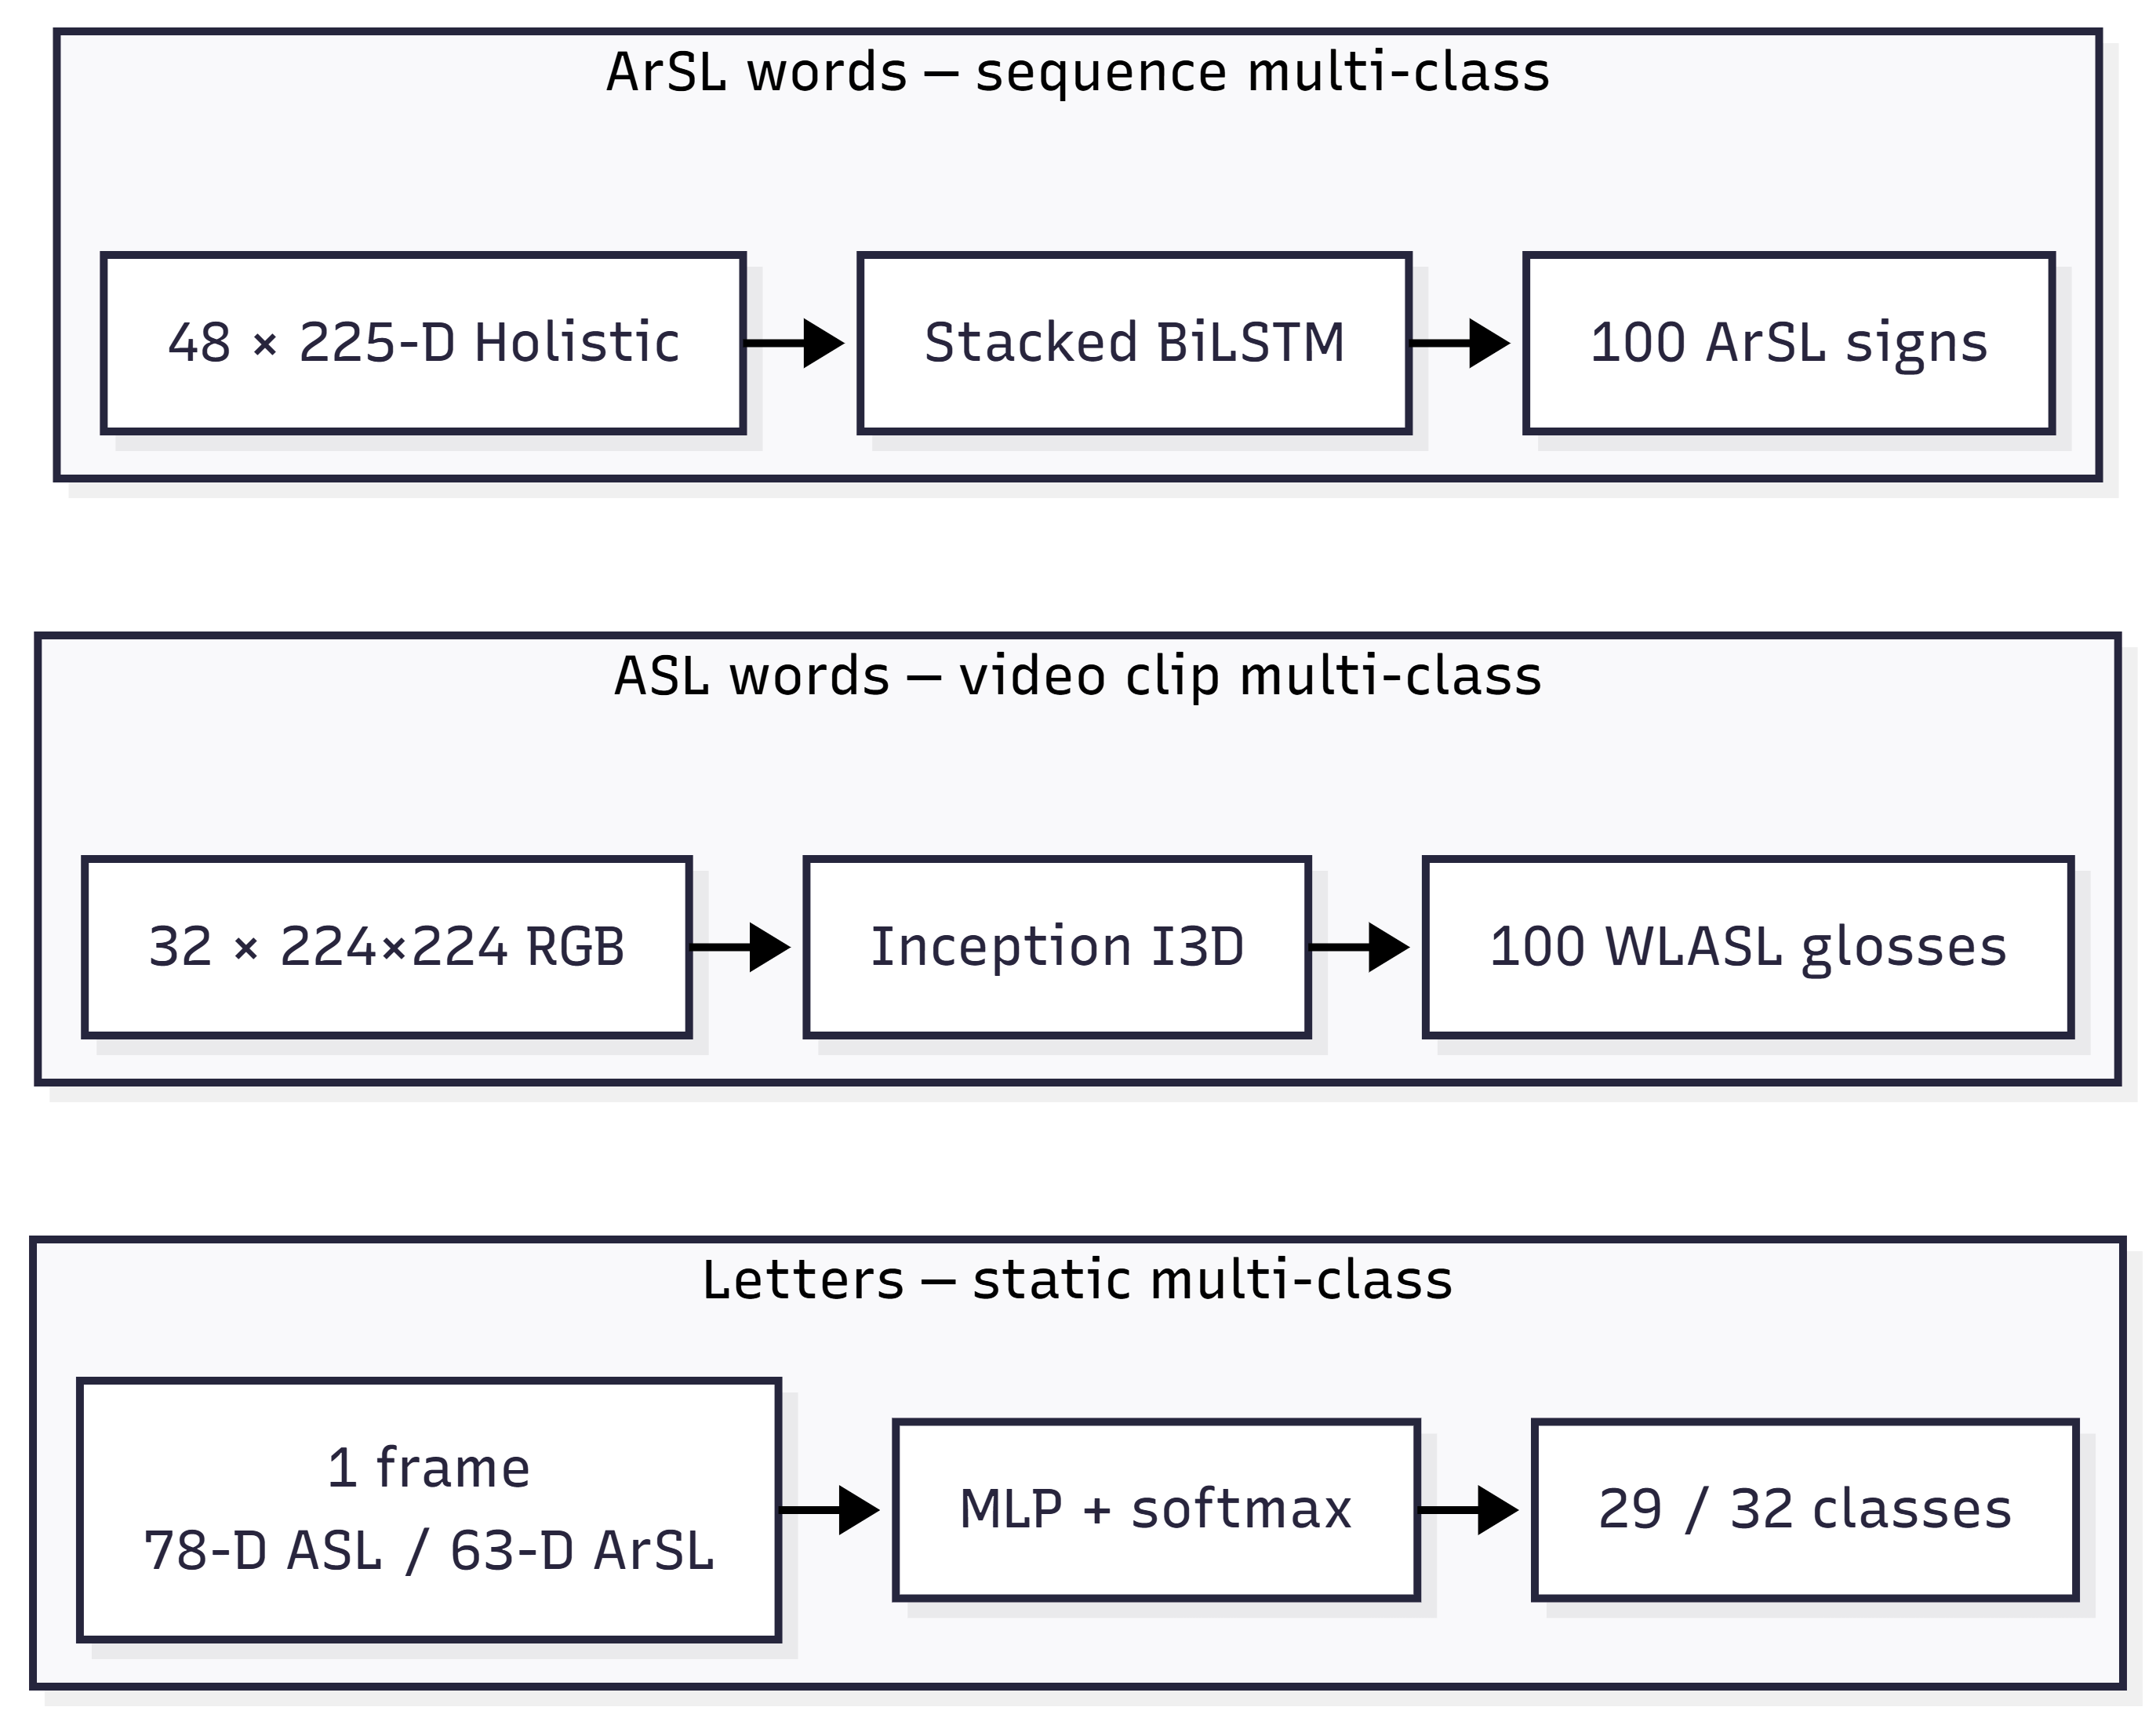
\includegraphics[width=0.95\textwidth]{images/fig_2-3_ml_paradigms.png}
\caption{Supervised machine-learning paradigms mapped to Eshara's four models (cf.\ Table~\ref{tab:ml-paradigms}): static MLPs for letters, Inception I3D for ASL words, and a stacked BiLSTM for ArSL words.}
\label{fig:ml-paradigms}
\end{figure}
\vspace{0.2cm}

\noindent As illustrated in Figure~\ref{fig:ml-paradigms}, input structure (single vector, RGB clip, or landmark sequence) determines the classifier family for each model. Full tensor shapes and training objectives are derived in Chapters~3 and~4.\par\vspace{0.2cm}

\noindent\textbf{2.2.3\quad Families of neural networks in SLR:}\par
\addcontentsline{toc}{subsection}{\numberline{2.2.3}Families of neural networks in SLR:}
\vspace{0.3cm}

\noindent Deep learning for SLR draws on several architectural families, each suited to a different input structure~\cite{adaloglou2022comprehensive,rastgoo2021survey}.\par\vspace{0.3cm}

\noindent \textbf{Multi-layer perceptrons (MLPs)} are feed-forward networks: information flows input $\rightarrow$ hidden layers $\rightarrow$ softmax output with no memory of previous frames. They are the standard choice when $T{=}1$ and latency must be minimal~\cite{ioffe2015batchnorm,srivastava2014dropout}.\par\vspace{0.3cm}

\noindent \textbf{Convolutional neural networks (CNNs)} apply learned filters over spatial dimensions (height $\times$ width of an image, or pseudo-spatial layouts of landmarks). CNNs dominated pixel-based SLR in the 2014--2018 period~\cite{he2016deep,sandler2018mobilenetv2}. Eshara uses CNNs in early letter-image experiments and in the deployed ASL word model (Inception I3D); letter models convert images to landmarks and train MLPs instead~\cite{zhang2020mediapipe,li2020wlasl}.\par\vspace{0.3cm}

\noindent \textbf{Recurrent neural networks (RNNs) and LSTMs} maintain a hidden state that is updated at each time step, allowing the model to aggregate information across frames. Long Short-Term Memory (LSTM) units avoid vanishing gradients on sequences of 32--48 frames~\cite{hochreiter1997long,pascanu2013difficulty}. Bidirectional LSTMs (BiLSTMs) read the sequence forward and backward so that both sign onset and completion inform the decision~\cite{schuster1997bidirectional,pigou2018sign}.\par\vspace{0.3cm}

\noindent \textbf{Attention mechanisms} learn which time steps (or feature subspaces) matter most for classification. Additive attention pools a weighted sum of BiLSTM outputs~\cite{bahdanau2015neural}; multi-head attention learns several attention patterns in parallel~\cite{vaswani2017attention}. Attention variants appear in the WLASL literature~\cite{li2020wlasl}; the ArSL word model uses a plain stacked BiLSTM without an explicit attention module~\cite{sidig2021karsl}.\par\vspace{0.3cm}

\noindent \textbf{Transformers} replace recurrence with self-attention over the full sequence. They achieve state-of-the-art results on large continuous SLR corpora but typically require more data and compute than BiLSTM models on graduation-scale vocabularies~\cite{vaswani2017attention,duarte2021how2sign}. Transformers are cited for context but are not the graduation architecture choice.\par\vspace{0.2cm}

\noindent\textbf{2.2.4\quad Training, validation, and evaluation:}\par
\addcontentsline{toc}{subsection}{\numberline{2.2.4}Training, validation, and evaluation:}
\vspace{0.3cm}

\noindent Supervised models are trained by minimising a \textbf{loss function} on labelled data. Eshara uses \textbf{categorical cross-entropy} for all four models: the network outputs a probability distribution over classes, and training penalises assignments that assign low probability to the correct label~\cite{szegedy2016rethinking,kingma2015adam}. Optimisation uses the Adam algorithm with mini-batches; dropout and batch normalisation reduce overfitting~\cite{kingma2015adam,ioffe2015batchnorm,srivastava2014dropout}.\par\vspace{0.2cm}

\noindent Data are partitioned into \textbf{training}, \textbf{validation}, and \textbf{test} sets. Training updates weights; validation selects hyperparameters and early-stopping checkpoints; test evaluation is run once on held-out data to report thesis metrics. Letter models use random image splits; the ArSL word model is evaluated on a held-out KArSL test partition (SignID 71--170)~\cite{sidig2021karsl}. Reporting validation accuracy alone would be optimistic; the thesis headline numbers are always \textbf{test-set} Top-1, Top-5 (word models), and macro-F1~\cite{li2020wlasl,rastgoo2021survey}.\par\vspace{0.2cm}

\noindent The following table summarises evaluation metrics common in the SLR literature and explains which Eshara reports in Chapter~6. Word models with imbalanced or scarce per-class data benefit from Top-5 and macro-F1 in addition to Top-1~\cite{li2020wlasl,sidig2021karsl}.\par\vspace{0.2cm}

\begin{table}[H]
\centering
\caption{Evaluation metrics in SLR literature and in Eshara.}
\label{tab:eval-metrics}
\small
\begin{tabular}{|P{2.8cm}|P{3.2cm}|P{3.0cm}|}
\hline
\multicolumn{1}{|c|}{\textbf{Metric}} & \multicolumn{1}{|c|}{\textbf{Typical use in SLR}} & \multicolumn{1}{|c|}{\textbf{Eshara usage}}\\
\hline
Top-1 accuracy & Isolated classification & All four models (headline) \\
\hline
Top-5 accuracy & Large / imbalanced vocabularies & ASL + ArSL word models \\
\hline
Macro-F1 & Per-class balance (scarce classes) & Word models; ArSL graduation headline \\
\hline
Weighted-F1 & Sample-frequency weighting & Reported alongside macro-F1 (ArSL) \\
\hline
WER / CER & Continuous SLR, translation & Not used (isolated scope) \\
\hline
Signer-independent acc. & Generalisation across signers & Future work; held-out clip splits for word models \\
\hline
\end{tabular}
\end{table}
\vspace{0.2cm}

\noindent\textbf{2.2.5\quad Isolated SLR versus continuous SLR as ML problems:}\par
\addcontentsline{toc}{subsection}{\numberline{2.2.5}Isolated SLR versus continuous SLR as ML problems:}
\vspace{0.3cm}

\noindent It is useful to distinguish two \textbf{problem formulations} in the literature. \emph{Isolated sign recognition} is standard multi-class classification: each clip contains one known sign, and the model outputs one label. \emph{Continuous sign recognition} is sequence-to-sequence learning: an unsegmented video may contain many signs, and the model must output a sequence of gloss labels with correct boundaries~\cite{koller2020weakly,camgoz2018neural}. Continuous SLR additionally requires \textbf{segmentation} (detecting where one sign ends) and often \textbf{language modelling} across glosses. Eshara solves only the isolated formulation: the user pauses between signs, and the web UI buffers one letter pose or one word motion window at a time. This reduces problem complexity and matches the educational and assistive use cases targeted in graduation scope~\cite{li2020wlasl,sidig2021karsl,duarte2021how2sign}.\par\vspace{0.2cm}

\begin{figure}[H]
\centering
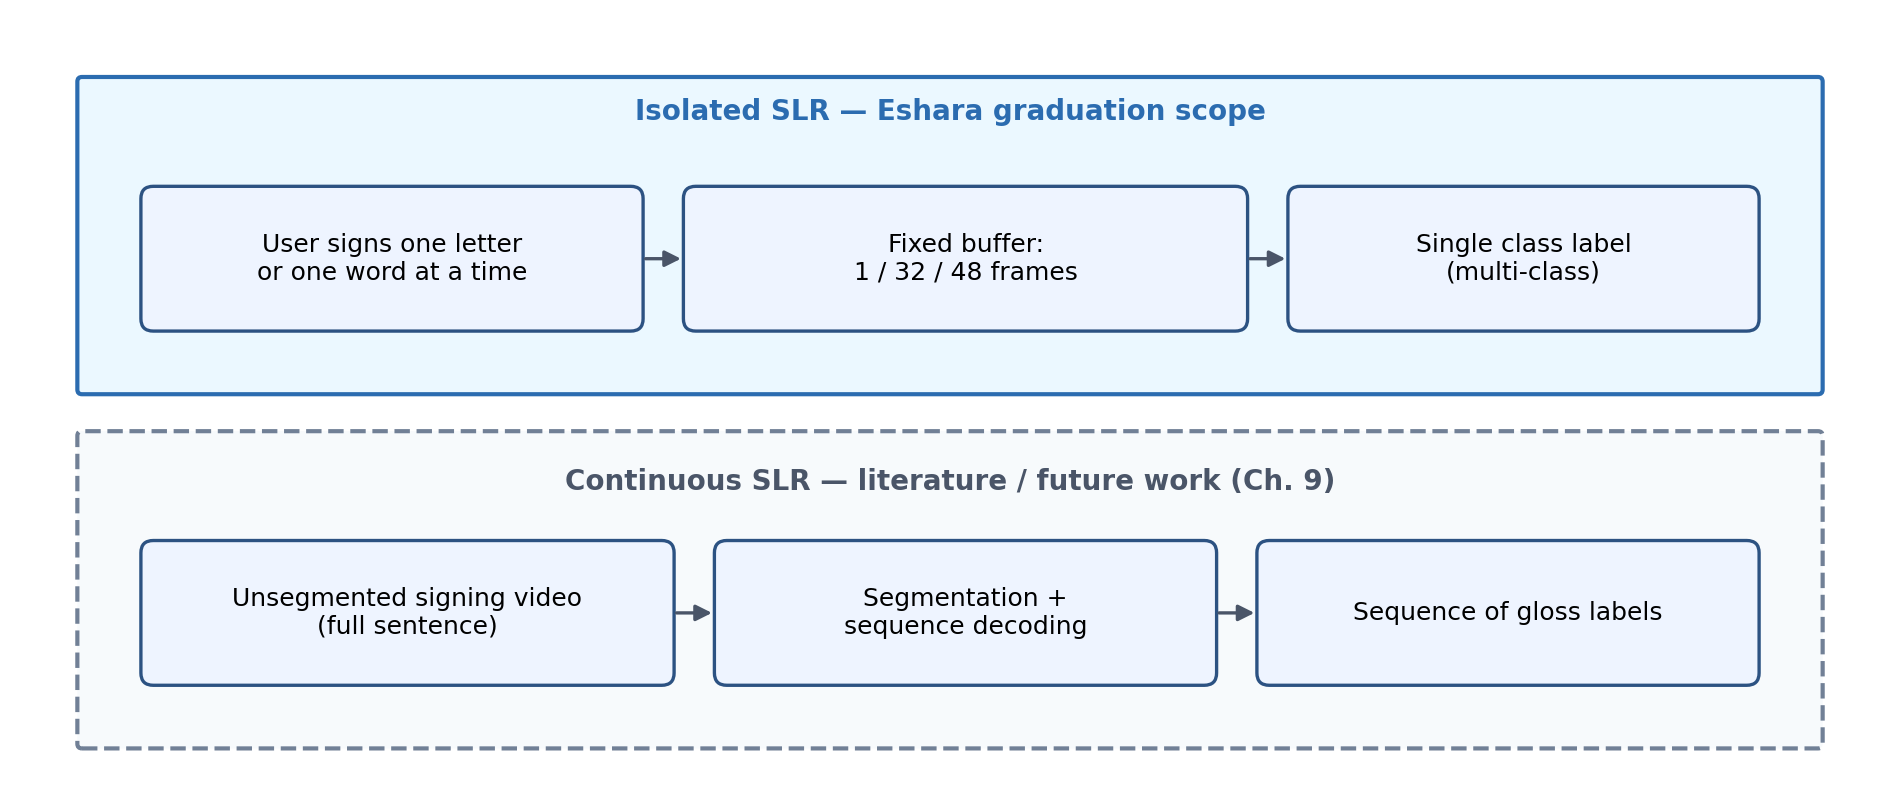
\includegraphics[width=0.88\textwidth]{images/fig_2-4_isolated_vs_continuous.png}
\caption{Isolated versus continuous sign-language recognition as machine-learning problem formulations. Eshara implements isolated classification only; continuous gloss decoding is deferred to Chapter~9.}
\label{fig:isolated-vs-continuous}
\end{figure}
\vspace{0.2cm}

\noindent As illustrated in the following figure, the fixed-buffer interaction model used in Eshara contrasts with the segmentation and sequence-decoding requirements of continuous SLR benchmarks such as How2Sign and RWTH-PHOENIX~\cite{duarte2021how2sign,forster2014rwth}.\par\vspace{0.2cm}

\noindent\textbf{2.2.6\quad Preprocessing, normalisation, and augmentation:}\par
\addcontentsline{toc}{subsection}{\numberline{2.2.6}Preprocessing, normalisation, and augmentation:}
\vspace{0.3cm}

\noindent Landmark-based SLR pipelines share a common preprocessing stage before neural classification~\cite{zhang2020mediapipe,deng2024skeleton,adaloglou2022comprehensive}. Landmarks are typically \textbf{centred} on a reference joint (wrist or shoulder) and \textbf{scale-normalised} by inter-joint distance so that signer height and camera distance have reduced influence. \textbf{Missing} detections from occlusion are zero-filled or linearly interpolated; the live web client applies the same convention as offline training for consistency~\cite{zhang2020mediapipe}. \textbf{Standardisation} (subtract training mean, divide by training standard deviation per feature dimension) is common in the literature and is fit on the training split only to prevent test leakage; Eshara's letter MLPs and deployed word models instead rely on geometric normalisation and in-network batch normalisation without external \texttt{StandardScaler} checkpoints (Chapters~3--4).\par\vspace{0.3cm}

\noindent \textbf{Data augmentation} is widely used when per-class sample counts are low~\cite{perez2017augmentation,sidig2021karsl}. Image-based SLR applies spatial transforms (rotation, crop, colour jitter) to hand crops; sequence-based SLR may apply temporal jitter, frame dropout, or additive noise on landmark trajectories. Letter models rely on large balanced image corpora; ASL word I3D uses pretrained WLASL weights with standard frame-level normalisation at inference.\par\vspace{0.3cm}
\clearpage
% --- 2.3 COMPUTER VISION APPROACHES ---
\noindent\textbf{2.3\quad COMPUTER VISION APPROACHES TO SLR}\par
\addcontentsline{toc}{section}{\numberline{2.3}COMPUTER VISION APPROACHES TO SLR}
\vspace{0.2cm}

\noindent\textbf{2.3.1\quad Image-Based Convolutional Methods:}\par
\addcontentsline{toc}{subsection}{\numberline{2.3.1}Image-Based Convolutional Methods:}
\vspace{0.3cm}

\noindent Deep convolutional networks such as ResNet~\cite{he2016deep}, MobileNetV2~\cite{sandler2018mobilenetv2,howard2017mobilenets}, and EfficientNet~\cite{tan2019efficientnet} established strong baselines for image classification by learning spatial hierarchies of visual features. Several sign-language studies apply similar architectures to hand images or signing clips, reporting high accuracy when camera viewpoint, background, and signer identity are constrained~\cite{rastgoo2021survey,pigou2018sign,huang2018attention}. Residual connections~\cite{he2016deep} ease optimisation of deep stacks; inverted residuals and depthwise separable convolutions~\cite{sandler2018mobilenetv2} reduce multiply--accumulate cost, which is attractive for edge deployment. EfficientNet~\cite{tan2019efficientnet} further trades off depth, width, and resolution through compound scaling.\par\vspace{0.2cm}

\noindent Despite strong offline metrics, three limitations motivate Eshara's \textbf{hybrid input design} for live webcam use. \textbf{Generalisation:} a model trained on cropped dataset images may degrade on new backgrounds, skin tones, jewellery, or lower-resolution webcams because pixel statistics shift while kinematic structure remains stable~\cite{zhang2020mediapipe}. \textbf{Compute:} letter and ArSL word paths classify compact landmark vectors (63--225 dimensions per frame) on modest hardware, whereas ASL word I3D requires batched 3D convolutions on 32-frame RGB clips~\cite{sandler2018mobilenetv2,li2020wlasl}. \textbf{Pipeline mismatch:} if training uses static dataset photographs but inference uses a live camera, the system must solve two domain-shift problems simultaneously (vision appearance and temporal sampling) rather than one (landmark noise only).\par\vspace{0.2cm}

\noindent The following table records vision pipelines explored during development and the rationale for the graduation choice. During early experimentation, MobileNetV2 was trained on hand-cropped letter images. Although accuracy on fixed-view dataset images was competitive, the domain gap between curated photographs and live webcam capture motivated a unified landmark representation instead. Eshara's letter pipelines illustrate this pragmatic compromise. The ASL and ArSL letter corpora are distributed as static hand images~\cite{akash2019aslalphabet,arthur2018arasl2018}, yet both are converted offline to MediaPipe hand landmarks --- 78-D engineered vectors for ASL and 63-D raw vectors for ArSL --- and trained with the same MLP \emph{architectural family} but language-specific hidden widths and hyperparameters (Chapter~3). At runtime the same feature conventions are preserved through the deployed inference path, reducing train--serve drift. This design follows the broader literature consensus that skeleton features narrow the domain gap between curated datasets and casual camera capture~\cite{zhang2020mediapipe,rastgoo2021survey,adaloglou2022comprehensive,deng2024skeleton}.\par\vspace{0.2cm}

\begin{table}[H]
\centering
\caption{Vision pipelines considered during Eshara development.}
\label{tab:approaches-considered}
\small
\begin{tabular}{|P{2.8cm}|P{3.2cm}|P{3.0cm}|}
\hline
\multicolumn{1}{|c|}{\textbf{Approach}} & \multicolumn{1}{|c|}{\textbf{Explored in project?}} & \multicolumn{1}{|c|}{\textbf{Outcome}}\\
\hline
Sensor gloves / Kinect depth & No (graduation scope) & Historical; not deployable on standard webcams \\
\hline
MobileNetV2 on hand images & Yes (early trials) & Strong offline; webcam domain gap \\
\hline
Pixel CNN / ResNet on video & Limited trials & Heavy; mismatched live pipeline \\
\hline
Landmarks + MLP (letters) & \textbf{Yes --- deployed} & Unified train/live representation \\
\hline
I3D on RGB (ASL words) & \textbf{Yes --- deployed} & 32-frame video clips \\
\hline
Landmarks + BiLSTM (ArSL words) & \textbf{Yes --- deployed} & 48-frame sequences \\
\hline
Full Transformer on words & Trial experiments & VRAM/data limits on graduation GPU \\
\hline
Single multilingual model & No & Incompatible label spaces (EN$\neq$AR) \\
\hline
\end{tabular}
\end{table}
\vspace{0.2cm}

\noindent\textbf{2.3.2\quad Skeleton and Landmark Methods:}\par
\addcontentsline{toc}{subsection}{\numberline{2.3.2}Skeleton and Landmark Methods:}
\vspace{0.3cm}

\noindent MediaPipe Hands uses a two-stage pipeline: a palm detector proposes hand regions, and a landmark regressor outputs 21 three-dimensional points per hand in normalised image coordinates~\cite{zhang2020mediapipe}. Each point carries $(x,y,z)$ relative to the hand bounding box, yielding $21 \times 3 = 63$ values per frame per hand. For finger-spelling, this single-frame vector is sufficient because letter signs are quasi-static poses: the classifier decision depends on fingertip configuration rather than long-horizon motion~\cite{akash2019aslalphabet,arthur2018arasl2018}. Word signs, by contrast, involve trajectory, two-handed coordination, facial grammar, and upper-body motion~\cite{li2020wlasl,sidig2021karsl}. Eshara therefore uses three feature regimes matched to task complexity, summarised in Table~\ref{tab:feature-vectors}.\par\vspace{0.2cm}

\begin{table}[H]
\centering
\caption{Feature-vector composition used by each Eshara model.}
\label{tab:feature-vectors}
\small
\begin{tabular}{|P{2.6cm}|r|r|r|P{3.8cm}|}
\hline
\multicolumn{1}{|c|}{\textbf{Model}} & \multicolumn{1}{|c|}{\textbf{Dim./frame}} & \multicolumn{1}{|c|}{\textbf{Frames}} & \multicolumn{1}{|c|}{\textbf{Tensor shape}} & \multicolumn{1}{|c|}{\textbf{Input source}}\\
\hline
ASL Letter MLP & 78 & 1 & $(78,)$ & MediaPipe Hands (engineered) \\
\hline
ArSL Letter MLP & 63 & 1 & $(63,)$ & MediaPipe Hands (raw) \\
\hline
ASL Word I3D & 224$\times$224 RGB & 32 & $(32, 224, 224, 3)$ & Raw webcam frames \\
\hline
ArSL Word BiLSTM & 225 & 48 & $(48, 225)$ & MediaPipe Holistic (normalised) \\
\hline
\end{tabular}
\end{table}
\vspace{0.2cm}

\noindent The ASL word model (Inception I3D) does not use landmarks: it consumes \textbf{raw RGB frames} ($32 \times 224 \times 224 \times 3$) normalised to $[-1,1]$. No MediaPipe extraction is required at inference time; the client buffers 32 centre-cropped frames and transmits them as encoded image data~\cite{li2020wlasl,zhang2020mediapipe}. The ArSL word model uses a \textbf{225-dimensional} normalised Holistic vector per frame: body pose ($33 \times 3 = 99$) centred on the nose, left hand ($21 \times 3 = 63$) centred on its wrist, and right hand ($21 \times 3 = 63$) centred on its wrist, giving $99 + 63 + 63 = 225$~\cite{sidig2021karsl,bazarevsky2020blazepose}. This body-relative normalisation reduces sensitivity to signer distance and height. The 48-frame window reflects the average sign duration in KArSL word clips~\cite{sidig2021karsl}.\par\vspace{0.2cm}

\noindent Before model input, landmarks are centred and scale-normalised (typically relative to wrist or shoulder width) so that signer body size and distance from the camera have reduced influence. Missing landmarks from occlusion are zero-filled or interpolated in the training pipeline; the deployed inference services apply the same convention for consistency~\cite{zhang2020mediapipe}. Landmark pipelines offer three engineering advantages emphasised in the literature but rarely demonstrated together in deployed bilingual systems. First, they require less labelled video than pixel-level models because the input dimensionality is orders of magnitude smaller~\cite{rastgoo2021survey,adaloglou2022comprehensive}. Second, they support privacy-preserving designs on letter and ArSL word paths: compact features are processed per request, while ASL word mode sends encoded frame buffers instead of continuous raw video. Third, MediaPipe provides runtimes suitable for real-time extraction in practical web systems~\cite{mediapipeweb,zhang2020mediapipe}.\par\vspace{0.2cm}

\noindent OpenPose remains a widely cited baseline but is heavier and lacks a first-class browser runtime~\cite{cao2019openpose}. MediaPipe Holistic (543 raw landmarks) and MoveNet (17 body keypoints) were evaluated during development; Holistic proved too slow for sustained live word recognition on laptop hardware at the target frame rate, while MoveNet lacks the dual-hand detail required for finger-spelling~\cite{yu2021movenet,bazarevsky2020blazepose}. as compared in Table~\ref{tab:pose-frameworks} (Section~2.5), which compares these frameworks quantitatively.\par\vspace{0.2cm}

\begin{figure}[H]
\centering
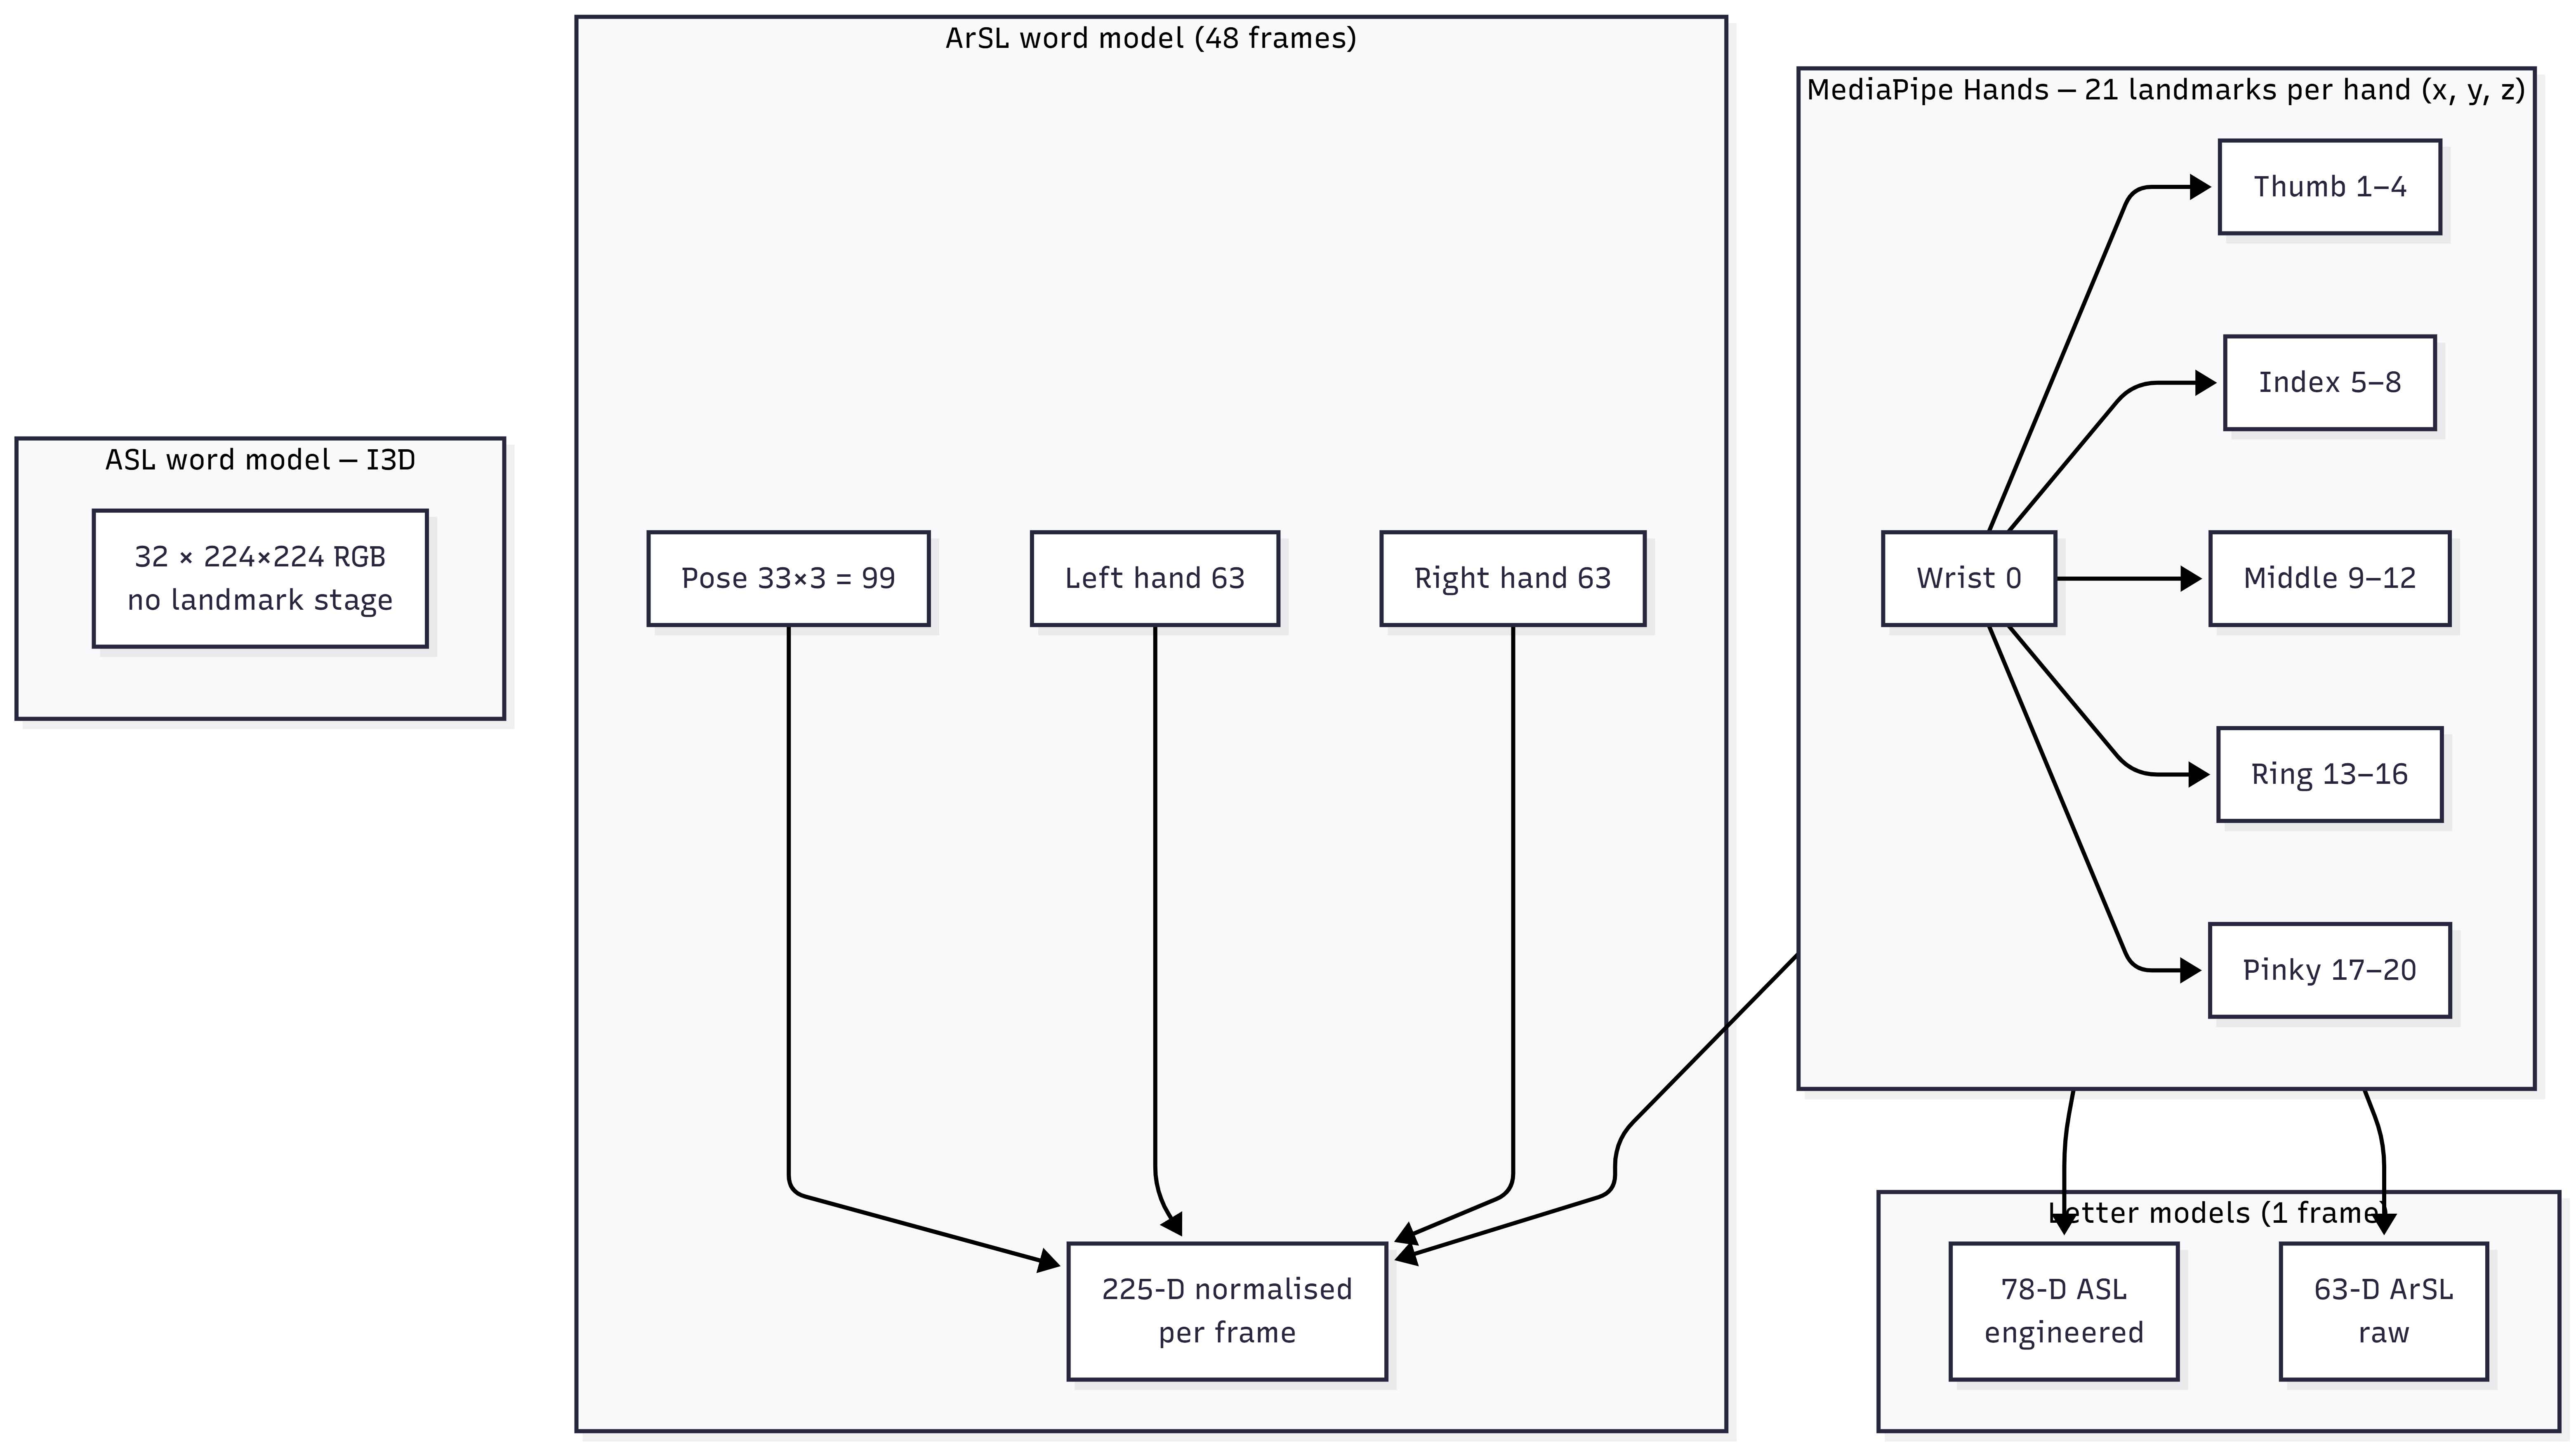
\includegraphics[width=0.88\textwidth]{images/fig_2-2_hand_landmarks.png}
\caption{MediaPipe hand landmarks (63-D per frame) and extension to normalised pose+hands feature vectors used by the ArSL word model (225-D). The ASL word model (I3D) consumes raw RGB frames rather than landmarks.}
\label{fig:hand-landmarks}
\end{figure}
\vspace{0.2cm}

\noindent As illustrated in Figure~\ref{fig:hand-landmarks}, finger-spelling needs only the 21-point hand mesh, whereas ArSL word recognition concatenates body pose and both hands into a 225-D normalised vector per frame. ASL word recognition bypasses landmarks entirely and feeds raw RGB clips into a pretrained I3D network~\cite{zhang2020mediapipe,bazarevsky2020blazepose,mediapipeweb,li2020wlasl}.\par\vspace{0.2cm}

\noindent\textbf{2.3.3\quad Hybrid CNN--RNN and Continuous SLR:}\par
\addcontentsline{toc}{subsection}{\numberline{2.3.3}Hybrid CNN--RNN and Continuous SLR:}
\vspace{0.3cm}

\noindent For sentence-level tasks, the dominant pattern is a visual encoder followed by a sequence model. Neural sign-language translation (SLT) systems pair convolutional front ends with recurrent or attention decoders to map signing video to spoken-language text without an intermediate gloss step in some architectures~\cite{camgoz2018neural}. Weakly supervised continuous sign-language recognition (CSLR) further shows that gloss-level alignment can be learned from untrimmed broadcast footage when only sentence-level weak labels are available~\cite{koller2020weakly}. Large-scale benchmarks such as How2Sign provide hundreds of hours of continuous American Sign Language aligned with English subtitles for this research line~\cite{duarte2021how2sign}, while RWTH-PHOENIX-Weather serves a similar role for German Sign Language~\cite{forster2014rwth}.\par\vspace{0.2cm}

\noindent Continuous systems must solve \emph{segmentation} (where one sign ends and the next begins) in addition to \emph{classification} (which sign is being performed). Isolated classifiers sidestep segmentation by asking the user to pause between signs --- a deliberate interaction pattern suitable for a graduation web demo and for educational finger-spelling practice. Eshara word models therefore classify fixed-length inputs --- 32-frame RGB clips for ASL words or 48-frame landmark sequences for ArSL words --- into a closed vocabulary rather than decoding unbounded gloss sequences. This is a well-studied stepping stone toward sentence-level systems and matches the interaction model of a user deliberately signing one word at a time in front of a webcam~\cite{li2020wlasl,sidig2021karsl,pigou2018sign}.\par\vspace{0.3cm}

% --- 2.4 DEEP-LEARNING ARCHITECTURES ---
\noindent\textbf{2.4\quad DEEP-LEARNING ARCHITECTURES}\par
\addcontentsline{toc}{section}{\numberline{2.4}DEEP-LEARNING ARCHITECTURES}
\vspace{0.2cm}

\noindent The four Eshara models span three architectural families introduced in Section~2.2: feed-forward MLPs for static letters, a 3D CNN (Inception I3D) for ASL words, and a stacked BiLSTM for ArSL words. This section states each family at a \textbf{conceptual} level only --- enough to follow the literature review. Full tensor layouts, layer dimensions, normalisation steps, loss functions, and training protocols are derived in Chapter~3 (letters) and Chapter~4 (words).\par\vspace{0.2cm}

\noindent\textbf{2.4.1\quad Multi-Layer Perceptrons (letter models):}\par
\addcontentsline{toc}{subsection}{\numberline{2.4.1}Multi-Layer Perceptrons (letter models):}
\vspace{0.3cm}

\noindent An MLP maps a single input vector $\mathbf{x}$ to a class label through a stack of fully connected layers. Each hidden layer applies an affine transform followed by a non-linear activation (ReLU in Eshara), optionally with batch normalisation and dropout for regularisation~\cite{ioffe2015batchnorm,srivastava2014dropout}. The final layer outputs a score vector $\mathbf{z}$ over $C$ classes; softmax converts these scores into a probability distribution and the predicted class is $\hat{y} = \arg\max_k P(y{=}k \mid \mathbf{x})$~\cite{szegedy2016rethinking}. Because finger-spelled letters are quasi-static poses, no recurrence is required: one 78-D (ASL) or 63-D (ArSL) vector per frame suffices. Chapter~3 specifies the exact layer widths ($256 \rightarrow 128 \rightarrow 64 \rightarrow C$ for ASL; $512 \rightarrow 256 \rightarrow 64 \rightarrow C$ for ArSL), the ASL 78-D feature-engineering equations, batch-norm and dropout placement, the cross-entropy loss, and the $\sim$49\,k / $\sim$183\,k parameter counts for Models~1 and~2.\par\vspace{0.2cm}

\noindent\textbf{2.4.2\quad Inception I3D (ASL word model):}\par
\addcontentsline{toc}{subsection}{\numberline{2.4.2}Inception I3D (ASL word model):}
\vspace{0.3cm}

\noindent Inception I3D (Inflated 3D ConvNet) extends 2D Inception modules to video by convolving jointly over spatial height, width, and time~\cite{li2020wlasl}. The ASL word model consumes a clip of $T{=}32$ centre-cropped RGB frames ($224 \times 224$ per frame), learns spatio-temporal filters without hand-crafted landmarks, and outputs logits over 100 WLASL glosses. Per-frame predictions are averaged over time before argmax classification. Eshara deploys a pretrained Inception I3D checkpoint (\texttt{asl\_word\_i3d.pt}) rather than training from scratch within graduation GPU limits. Chapter~4 documents clip buffering, $[-1,1]$ frame normalisation, and the Model~3 architecture; Chapter~5 documents the live web pipeline.\par\vspace{0.2cm}

\noindent\textbf{2.4.3\quad Bidirectional LSTM (ArSL word model):}\par
\addcontentsline{toc}{subsection}{\numberline{2.4.3}Bidirectional LSTM (ArSL word model):}
\vspace{0.3cm}

\noindent A Long Short-Term Memory (LSTM) network maintains a hidden state that is updated at each time step, allowing the model to aggregate motion across a signing clip~\cite{hochreiter1997long,pascanu2013difficulty}. Gated units control how much past context is retained or forgotten at each frame. A \textbf{bidirectional} LSTM reads the sequence forward and backward and concatenates both hidden states at each step, so sign onset and completion both inform the final decision~\cite{schuster1997bidirectional,pigou2018sign}. The ArSL word model stacks two BiLSTM layers on 48-frame sequences of 225-D normalised Holistic vectors and classifies into 100 Arabic sign classes with a dense softmax head; no explicit attention module is used. Chapter~4 gives the full gate equations, tensor shapes $(48, 225)$, nose/wrist normalisation, and evaluation on the held-out KArSL test partition (SignID 71--170).\par\vspace{0.2cm}

\noindent\textbf{2.4.4\quad Attention and transformers (literature context):}\par
\addcontentsline{toc}{subsection}{\numberline{2.4.4}Attention and transformers (literature context):}
\vspace{0.3cm}

\noindent \textbf{Attention} mechanisms learn which time steps in a clip carry the most discriminative motion --- useful when neutral rest frames precede or follow the stroke phase~\cite{bahdanau2015neural,li2020wlasl,huang2018attention}. Additive and multi-head variants appear in the WLASL literature but are \textbf{not} part of Eshara's graduation architectures. \textbf{Transformers} replace recurrence with self-attention over the full sequence and achieve strong results on large continuous-SLR corpora, but typically require more data and compute than BiLSTM or I3D models at graduation vocabulary scale~\cite{vaswani2017attention,duarte2021how2sign}. They are cited here for context only.\par\vspace{0.3cm}

% --- 2.5 POSE ESTIMATION (TABLE) ---
\noindent\textbf{2.5\quad POSE-ESTIMATION FRAMEWORKS}\par
\addcontentsline{toc}{section}{\numberline{2.5}POSE-ESTIMATION FRAMEWORKS}
\vspace{0.2cm}

\noindent The following table compares frameworks considered for Eshara. Selection criteria were: (i)~availability of a maintained browser/WASM build; (ii)~sustained $\geq$25\,FPS on a mid-range laptop webcam stream; (iii)~compatibility with dual-hand finger-spelling; and (iv)~sufficient body keypoints for ArSL word motion~\cite{zhang2020mediapipe,bazarevsky2020blazepose,mediapipeweb,cao2019openpose}.\par\vspace{0.2cm}

\begin{table}[H]
\centering
\caption{Comparison of pose-estimation frameworks.}
\label{tab:pose-frameworks}
\small
\begin{tabular}{|P{2.5cm}|c|c|c|P{4.8cm}|}
\hline
\multicolumn{1}{|c|}{\textbf{Framework}} & \multicolumn{1}{|c|}{\textbf{Landmarks}} & \multicolumn{1}{|c|}{\textbf{Typical FPS}} & \multicolumn{1}{|c|}{\textbf{Browser}} & \multicolumn{1}{|c|}{\textbf{Role in Eshara}}\\
\hline
MediaPipe Hands & 21 per hand & 30+ & Yes (WASM) & Letter models (78-D ASL / 63-D ArSL) \\
\hline
MediaPipe Holistic & 543 & 18 & Yes & Literature reference; ASL word uses I3D (raw RGB) \\
\hline
MediaPipe Pose + Hands & 33 + 21$\times$2 & 25+ & Yes (WASM) & ArSL word model (225-D normalised) \\
\hline
OpenPose & 25 body & 8 & No & Literature baseline \\
\hline
MoveNet & 17 & 40+ & Yes & Compared, not used \\
\hline
\end{tabular}
\end{table}
\vspace{0.2cm}

\noindent MediaPipe Hands satisfies real-time letter recognition with the lowest feature dimensionality. Holistic provides the richest context for ASL words but at higher per-frame cost; it is used offline and in the browser word mode where the user holds still briefly during a sign. Pose+Hands offers the best balance for ArSL graduation words: full torso and dual-hand coverage without the face mesh overhead. OpenPose is included as a historical baseline from the literature~\cite{cao2019openpose} but was not integrated because deployment targets the browser, not a C++ desktop server. MoveNet's 17-point skeleton is insufficient for distinguishing ArSL two-hand minimal pairs~\cite{yu2021movenet,sidig2021karsl}.\par\vspace{0.3cm}

% --- 2.6 DATASETS (TABLE) ---
\noindent\textbf{2.6\quad SIGN-LANGUAGE DATASETS}\par
\addcontentsline{toc}{section}{\numberline{2.6}SIGN-LANGUAGE DATASETS}
\vspace{0.2cm}

\noindent The following table summarises the corpora that ground the four Eshara models. A deliberate design constraint is that \textbf{each model maintains its own label space}; vocabularies are not shared across languages or tasks~\cite{li2020wlasl,sidig2021karsl}. This avoids impossible label alignment (an ASL gloss does not correspond to an ArSL gloss) and allows independent retraining when one corpus is updated.\par\vspace{0.2cm}

\begin{table}[H]
\centering
\caption{Sign-language datasets used or referenced in this work.}
\label{tab:datasets}
\small
\begin{tabular}{|P{2.4cm}|c|c|r|r|P{3.5cm}|}
\hline
\multicolumn{1}{|c|}{\textbf{Dataset}} & \multicolumn{1}{|c|}{\textbf{Lang.}} & \multicolumn{1}{|c|}{\textbf{Type}} & \multicolumn{1}{|c|}{\textbf{Classes}} & \multicolumn{1}{|c|}{\textbf{Samples}} & \multicolumn{1}{|c|}{\textbf{Role}}\\
\hline
ASL Alphabet (Kaggle) & ASL & Images & 29 & 87\,000 & ASL letter MLP \\
\hline
ArASL2018 & ArSL & Images & 32 & 54\,049 & ArSL letter MLP \\
\hline
WLASL-2000 & ASL & Video & 2000 & 21\,000 & 100-class I3D subset \\
\hline
KArSL-502 & ArSL & Video & 502 & 24\,000 & 100-class word subset (SignID 71--170) \\
\hline
How2Sign & ASL & Continuous & --- & 80\,h & Future work (Ch.~8) \\
\hline
RWTH-PHOENIX & DGS & Continuous & --- & --- & Comparison only \\
\hline
\end{tabular}
\end{table}
\vspace{0.2cm}

\noindent The following table highlights \textbf{class imbalance} and average samples per class --- a key reason Eshara reports macro-F1 and Top-5 for word models, uses a 100-class WLASL subset for I3D, and a 100-class KArSL word subset for the ArSL BiLSTM~\cite{li2020wlasl,sidig2021karsl}.\par\vspace{0.2cm}

\begin{table}[H]
\centering
\caption{Approximate class balance across Eshara training corpora.}
\label{tab:dataset-imbalance}
\small
\begin{tabular}{|P{2.8cm}|r|r|r|P{3.5cm}|}
\hline
\multicolumn{1}{|c|}{\textbf{Corpus (Eshara use)}} & \multicolumn{1}{|c|}{\textbf{Classes}} & \multicolumn{1}{|c|}{\textbf{Total samples}} & \multicolumn{1}{|c|}{\textbf{$\sim$Avg/class}} & \multicolumn{1}{|c|}{\textbf{Implication}}\\
\hline
ASL Alphabet & 29 & 87\,000 & $\sim$3\,000 & Balanced; Top-1 sufficient \\
\hline
ArASL2018 & 32 & 54\,049 & $\sim$1\,700 & Balanced; more confusion pairs \\
\hline
WLASL I3D subset & 100 & $\sim$3\,000 clips & 10--50 (varies) & I3D pretrained; Top-5 \\
\hline
KArSL word subset & 100 & $\sim$4\,800 seq. & $\sim$48 & BiLSTM; 99.62\,\% Top-1 \\
\hline
\end{tabular}
\end{table}
\vspace{0.2cm}

\noindent\textbf{Train/test splitting and leakage.} Random frame-level or clip-level shuffles on video corpora can \textbf{leak} adjacent segments from the same recording session into both training and test sets, producing optimistically high accuracy that does not generalise to new signing sessions~\cite{johnson2019signer,sidig2021karsl}. The ArSL word model is evaluated on a held-out KArSL test partition (SignID 71--170); the headline \textbf{99.62\,\%} Top-1 reported in Chapter~6 was obtained under this protocol. Letter image datasets contain independent photographs and use random stratified splits instead.\par\vspace{0.2cm}

\noindent\textbf{ASL Alphabet (Kaggle).} The dataset provides large-scale static hand images for 29 finger-spelling classes including control signs (\texttt{space}, \texttt{del}, \texttt{nothing})~\cite{akash2019aslalphabet}. With roughly 3\,000 images per class on average, it supports reliable MLP training and achieves high offline accuracy in project experiments. Limitations include studio-style backgrounds, limited signer diversity compared with field capture, and the absence of temporal motion required for word models. Motion letters J and Z are under-represented in live testing because they require trajectory, not a single pose.\par\vspace{0.2cm}

\noindent\textbf{ArASL2018.} This corpus is the primary public benchmark for Arabic finger-spelling, with 32 classes and 54\,049 images collected under relatively controlled indoor conditions~\cite{arthur2018arasl2018}. Visually similar letter pairs (for example \arTxt{ك} vs.\ \arTxt{ل} in Arabic signing) produce more inter-class confusion than in ASL, which motivates separate evaluation and a wider ArSL letter MLP head despite the shared architectural family (Chapter~3). The dataset does not cover ArSL word signs; a second corpus is required for word-level Arabic recognition.\par\vspace{0.2cm}

\noindent\textbf{WLASL-2000.} Li et al.\ introduced WLASL as a large-scale American Sign Language word dataset spanning 2\,000 glosses and roughly 21\,000 video clips sourced from public video portals~\cite{li2020wlasl}. Not every gloss has equal footage quality; broken URLs in the metadata reduce effective coverage. Eshara's ASL word model (Model~3) uses a \textbf{100-class WLASL subset}: 32-frame centre-cropped $224\!\times\!224$ RGB clips pass through a pretrained Inception I3D checkpoint (\texttt{asl\_word\_i3d.pt}) with a 100-way softmax head~\cite{li2020wlasl}. Using a pretrained checkpoint keeps deployment tractable within graduation GPU and timeline constraints.\par\vspace{0.2cm}

\noindent\textbf{KArSL-502 and the graduation word subset.} Sidig et al.\ published KArSL as a 502-class Arabic sign-language video corpus with approximately 24\,000 clips performed primarily by Saudi signers~\cite{sidig2021karsl}. Average samples per class are far smaller than ASL Alphabet's image counts, and regional dialect variation across the Arab world is not fully represented. Eshara uses a stacked \textbf{BiLSTM} over a \textbf{100-class Arabic word subset} (SignID 71--170 of KArSL) with 225-D nose- and wrist-normalised Holistic landmark sequences of 48 frames each, achieving \textbf{99.62\,\%} Top-1 on the held-out test set~\cite{sidig2021karsl}.\par\vspace{0.2cm}

\noindent\textbf{Continuous benchmarks (not used in graduation).} How2Sign~\cite{duarte2021how2sign} and RWTH-PHOENIX-Weather~\cite{forster2014rwth} are cited to position Eshara relative to sentence-level research. How2Sign aligns continuous ASL video with English subtitles and is the intended dataset for future continuous recognition experiments in Chapter~9. RWTH-PHOENIX demonstrates that European sign languages have received substantially more continuous-SLR infrastructure than ArSL, reinforcing the bilingual gap Eshara addresses at the isolated-sign level.\par\vspace{0.3cm}

% --- 2.7 BILINGUAL ---
\noindent\textbf{2.7\quad BILINGUAL AND ARABIC SIGN-LANGUAGE RESEARCH}\par
\addcontentsline{toc}{section}{\numberline{2.7}BILINGUAL AND ARABIC SIGN-LANGUAGE RESEARCH}
\vspace{0.2cm}

\noindent Published sign-language recognition systems are overwhelmingly monolingual, with American Sign Language and a small set of European sign languages (German Sign Language, British Sign Language) dominating the literature~\cite{rastgoo2021survey,forster2014rwth,sterpu2018sign}. Comprehensive surveys confirm rapid growth in deep-learning SLR methods but note persistent dataset imbalance across languages~\cite{adaloglou2022comprehensive,al2022sign}. Arabic Sign Language has received comparatively little attention despite substantial deaf and hard-of-hearing populations in the Arab world~\cite{who2024hearing}. The release of KArSL-502 in 2021 enabled reproducible ArSL word classification experiments~\cite{sidig2021karsl}, yet few works extend to letter-level finger-spelling, bilingual deployment, or production-grade web interfaces in the same publication.\par\vspace{0.2cm}

\noindent Recent ArSL research illustrates the dominant pixel-based and hybrid CNN--LSTM paradigms. Luqman and El-Alfy cascaded CNN and LSTM encoders on KArSL subsets (33, 100, and 190 signs), reporting $>$99\,\% accuracy on controlled splits~\cite{luqman2022cascaded}. Dabwan and Jadhav applied ConvLSTM and LRCN architectures to 28 KArSL classes with validation accuracy up to 95\,\%~\cite{dabwan2023cnnlstm}. Alsaadi et al.\ developed a real-time ArSL \emph{alphabet} recogniser using AlexNet on static images (94.81\,\% accuracy)~\cite{alsaadi2022arsla}. Noor et al.\ proposed a hybrid CNN--LSTM model on a small custom Saudi ArSL word set with MediaPipe landmark extraction in a cloud deployment~\cite{noor2024hybrid}. These works confirm growing ArSL interest but typically address \textbf{one language}, \textbf{one granularity} (letters \emph{or} words), and \textbf{offline or server-side video} --- not a unified bilingual web product.\par\vspace{0.2cm}

\noindent ArASL2018 addressed the letter-level gap for Arabic~\cite{arthur2018arasl2018}, and several CNN and LSTM papers report competitive accuracy on KArSL subsets, but these contributions typically target a single task (letters \emph{or} words) in a single language with offline batch evaluation. To the authors' knowledge, no prior open system combines ASL and ArSL recognition at both letter and word granularities within a single webcam-driven web application. Eshara is designed explicitly to fill that \emph{structural} gap --- four specialised models, one user interface --- rather than to incrementally improve top-1 accuracy on a single-language benchmark by a few percentage points~\cite{li2020wlasl,sidig2021karsl}.\par\vspace{0.2cm}

\noindent Arabic-specific engineering considerations include right-to-left user-interface layout for translated text output, right-hand dominance in several regional signing conventions, and dialect variation that a single national corpus cannot fully capture~\cite{sidig2021karsl,arthur2018arasl2018}. These factors motivate parallel language-specific models with independent vocabularies rather than a single multilingual classifier with a shared label space. A shared embedding space across languages would require aligned glosses and substantially more parallel data than this graduation project scope provides~\cite{camgoz2018neural}.\par\vspace{0.3cm}

% --- 2.8 DEPLOYMENT ---
\noindent\textbf{2.8\quad REAL-TIME WEB DEPLOYMENT}\par
\addcontentsline{toc}{section}{\numberline{2.8}REAL-TIME WEB DEPLOYMENT}
\vspace{0.2cm}

\noindent A persistent divide exists between recognition accuracy reported in offline experiments and systems people can actually use~\cite{rastgoo2021survey,sterpu2018sign}. Many papers stop at confusion matrices on held-out test clips and do not report end-to-end latency from camera capture to readable text on screen. Deployment-focused surveys note that fewer than one in five SLR papers describe a user-facing demo accessible outside the authors' laboratory~\cite{adaloglou2022comprehensive}.\par\vspace{0.2cm}

\noindent Eshara targets a deployable web architecture with the following runtime path: (1)~the browser captures webcam frames; (2)~the React client sends translation requests to a Node.js/Express gateway over HTTPS; (3)~the Node layer authenticates and forwards requests to internal FastAPI model services over HTTP~\cite{rfc9110,fastapi}; (4)~the inference service loads the correct model path for the selected language and mode; (5)~predictions are returned as JSON and rendered in the React UI~\cite{react}. Socket.IO is used for live chat messaging, while prediction requests are served through the HTTP \texttt{/predict} flow. For letter mode, a stability decoder applies majority voting over a short frame buffer and a hold timer before committing a character, preventing repeated glyphs from a single prolonged pose.\par\vspace{0.2cm}

\noindent Keeping feature extraction on the client limits privacy risk and bandwidth use: a 48-frame ArSL word packet transmits roughly $48 \times 225 \times 4 \approx 43$\,KB of floats per inference request, whereas uncompressed 720p video would exceed several megabytes per second~\cite{rfc6455}. This pattern mirrors industrial real-time inference but remains uncommon in academic sign-language literature, where server-side video upload and batch processing are still typical~\cite{camgoz2018neural,li2020wlasl}. Accessibility guidelines (WCAG~2.2) further motivate web delivery: users can access the tool from any modern browser without installing native applications~\cite{wcag22}.\par\vspace{0.2cm}

\noindent Graduation scope is \textbf{web-only}: no mobile application, no TensorFlow Lite on-device model, and no app-store deployment is claimed in this thesis~\cite{abadi2016tensorflow}. The hypothesis in Section~1.5.4 targets end-to-end latency of no more than 200\,ms from frame capture to displayed prediction on a standard laptop; Chapter~5 reports whether live web measurements support that target alongside the offline accuracy metrics of Chapter~6.\par\vspace{0.3cm}
\clearpage
% --- 2.9 RESEARCH GAP ---
\noindent\textbf{2.9\quad RESEARCH GAP AND PROJECT POSITIONING}\par
\addcontentsline{toc}{section}{\numberline{2.9}RESEARCH GAP AND PROJECT POSITIONING}
\vspace{0.2cm}

\noindent The following table positions Eshara against typical published systems. Direct numeric comparison of Top-1 accuracy is often misleading because vocabularies, splits, and input representations differ; the table therefore emphasises \textbf{structural} coverage (language, granularity, deployment)~\cite{rastgoo2021survey,li2020wlasl,sidig2021karsl}.\par\vspace{0.2cm}

\begin{table}[H]
\centering
\caption{Structural comparison with representative SLR research lines (not a claim of state-of-the-art rank).}
\label{tab:related-systems}
\footnotesize
\resizebox{\textwidth}{!}{%
\begin{tabular}{|l|c|c|c|c|c|}
\hline
\multicolumn{1}{|c|}{\textbf{System / line}} & \multicolumn{1}{|c|}{\textbf{Lang.}} & \multicolumn{1}{|c|}{\textbf{Letters}} & \multicolumn{1}{|c|}{\textbf{Words}} & \multicolumn{1}{|c|}{\textbf{Live web}} & \multicolumn{1}{|c|}{\textbf{Landmarks}}\\
\hline
Typical WLASL paper~\cite{li2020wlasl} & EN & No & Yes & Rare & Varies \\
\hline
KArSL CNN--LSTM works~\cite{dabwan2023cnnlstm,luqman2022cascaded} & AR & No & Yes & No & RGB/depth \\
\hline
ArASL2018 / ArSLA~\cite{arthur2018arasl2018,alsaadi2022arsla} & AR & Yes & No & Limited & RGB \\
\hline
Noor et al.\ hybrid~\cite{noor2024hybrid} & AR & Partial & Yes & Server/cloud & MediaPipe \\
\hline
\textbf{Eshara (this thesis)} & \textbf{EN+AR} & \textbf{Yes} & \textbf{Yes} & \textbf{Yes} & \textbf{Yes} \\
\hline
\end{tabular}%
}
\end{table}
\vspace{0.2cm}

\noindent The following table consolidates the gaps identified throughout this chapter and maps each to a concrete Eshara design decision. Chapters~3 and~4 detail the methodology; Chapter~6 reports whether the experimental results support the hypothesis stated in Section~1.5.4.\par\vspace{0.2cm}

\begin{table}[H]
\centering
\caption{Research gaps addressed by Eshara.}
\label{tab:research-gap}
\begin{tabular}{|p{0.40\textwidth}|p{0.52\textwidth}|}
\hline
\multicolumn{1}{|c|}{\textbf{Gap in the literature}} & \multicolumn{1}{|c|}{\textbf{Eshara response}}\\
\hline
ArSL word recognition is under-studied & ArSL word BiLSTM on KArSL 100-class word subset (SignID 71--170) \\
\hline
Most systems target letters \emph{or} words, not both & Four specialised models with mode selection in one web app \\
\hline
ASL-centric datasets and models dominate & Parallel ArSL pipelines for letters and words \\
\hline
Academic prototypes rarely reach end users & React + FastAPI web product with live webcam UI \\
\hline
Raw video commonly sent to servers & Client-side landmarks for letters + ArSL words (78/63/225-D); encoded frames for ASL word I3D \\
\hline
Single-model papers lack unified APIs & One inference backend serving four models \\
\hline
\end{tabular}
\end{table}
\vspace{0.2cm}

\noindent The literature review supports the central hypothesis of Chapter~1: a webcam-driven pipeline with four specialised deep-learning models and a unified web deployment can achieve reliable recognition across the targeted tasks. Chapter~6 evaluates this claim using Top-1 accuracy, Top-5 accuracy, and macro-F1 on held-out test sets for each model independently~\cite{li2020wlasl,sidig2021karsl}. The experiments test five implicit sub-claims: (i)~compact MLPs on hand landmarks suffice for letter finger-spelling (78-D engineered for ASL, 63-D raw for ArSL); (ii)~a pretrained I3D network recognises ASL words from buffered RGB clips; (iii)~a landmark-based BiLSTM recognises ArSL words from 225-D Holistic sequences; (iv)~the deployed feature-extraction and inference path generalises from dataset images/videos to live webcam input; and (v)~a three-tier web backend can serve heterogeneous models without degrading interactive latency~\cite{zhang2020mediapipe,fastapi,rfc6455}.\par\vspace{0.3cm}

% --- 2.10 MODEL COMPARISON ---
\noindent\textbf{2.10\quad COMPARISON OF ESHARA'S FOUR MODELS}\par
\addcontentsline{toc}{section}{\numberline{2.10}COMPARISON OF ESHARA'S FOUR MODELS}
\vspace{0.2cm}

\noindent The following table summarises how architecture, feature dimensionality, temporal window length, and vocabulary size are matched to each recognition task. This design matrix is the technical backbone of Eshara and is detailed further in Chapters~3 and~4 and evaluated in Chapter~6.\par\vspace{0.2cm}

\begin{table}[H]
\centering
\caption{Architecture comparison of Eshara's four graduation models.}
\label{tab:four-models}
\footnotesize
\resizebox{\textwidth}{!}{%
\begin{tabular}{|l|c|c|c|c|c|r|r|}
\hline
\multicolumn{1}{|c|}{\textbf{Model}} & \multicolumn{1}{|c|}{\textbf{Lang.}} & \multicolumn{1}{|c|}{\textbf{Task}} & \multicolumn{1}{|c|}{\textbf{Architecture}} & \multicolumn{1}{|c|}{\textbf{Features}} & \multicolumn{1}{|c|}{\textbf{Frames}} & \multicolumn{1}{|c|}{\textbf{Classes}} & \multicolumn{1}{|c|}{\textbf{$\sim$Params}}\\
\hline
ASL Letter MLP & EN & Letter & MLP & 78-D hand & 1 & 28 (29 corpus) & $\sim$49K \\
\hline
ArSL Letter MLP & AR & Letter & MLP & 63-D hand & 1 & 32 & $\sim$183K \\
\hline
ASL Word I3D & EN & Word & Inception I3D (3D CNN) & 224$\times$224 RGB & 32 & 100 & $\sim$12.5M \\
\hline
ArSL Word BiLSTM & AR & Word & Stacked BiLSTM & 225-D Holistic (norm.) & 48 & 100 & $\sim$255K \\
\hline
\end{tabular}%
}
\end{table}
\vspace{0.2cm}

\noindent Static finger-spelling requires only per-frame pose information, motivating compact MLP classifiers for both letter models despite different vocabularies and feature dimensions~\cite{akash2019aslalphabet,arthur2018arasl2018}. Word signs require temporal modelling: the ASL word model uses a pretrained Inception I3D consuming raw RGB clips because 3D convolutions capture the rich spatio-temporal patterns of English word signs without manual landmark engineering~\cite{li2020wlasl}; the ArSL word model uses 225-D normalised Holistic sequences over 48 frames, matched to KArSL signing duration and the 100-class Arabic word vocabulary~\cite{sidig2021karsl}. Letter MLPs are on the order of $10^4$--$10^5$ parameters; the ArSL word BiLSTM is $\sim$255K and the ASL word I3D is $\sim$12.5M parameters.\par\vspace{0.2cm}

\noindent No label space is shared across models; bilingual capability is implemented as parallel inference pipelines behind one web interface. The ArSL word model achieves \textbf{99.62\,\%} Top-1 on the held-out test set (100 classes, Chapter~6); the ASL word I3D reaches \textbf{65.89\,\%} Top-1 on the WLASL-100 benchmark (Chapter~6). Chapters~3 and~4 present methodology for each row in Table~\ref{tab:four-models}.\par\vspace{0.3cm}

\noindent\textbf{Chapter summary.} This literature review established the technological and scientific context for Eshara. Historically, SLR moved from instrumented gloves to pixel-based deep learning and finally to hybrid landmark- and video-based classifiers deployable on ordinary webcams (Section~2.1). Machine-learning foundations (Section~2.2) cast all four models as supervised classifiers --- static MLPs for letters, Inception I3D for ASL words, and a stacked BiLSTM for ArSL words --- evaluated with Top-1, Top-5, and macro-F1 under honest split protocols. Computer-vision evidence (Section~2.3) justified the hybrid input design; deep-learning architectures (Section~2.4) introduce the model families whose full equations and dimensions are derived in Chapters~3 and~4. Dataset scale and imbalance (Section~2.6) motivated the 100-class WLASL I3D subset and the 100-class KArSL word subset. Bilingual and ArSL-specific work (Section~2.7) confirmed a structural gap that Eshara fills with four specialised models behind one web interface. The following design decisions, justified above, are carried forward:\par\vspace{0.3cm}

\noindent (1)~Landmark-first feature pipelines for letters and ArSL words, with RGB clip inference for ASL words; (2)~78-D (ASL) and 63-D (ArSL) MLP letter heads in the same architectural family with language-specific widths; (3)~pretrained Inception I3D on 32-frame 224$\times$224 RGB clips for ASL words; (4)~stacked BiLSTM on 225-D normalised Holistic sequences (48 frames) for ArSL words; (5)~four independent vocabularies with no shared label space; (6)~isolated-sign interaction only; (7)~web-only three-tier deployment (React + Node/Express + FastAPI). Chapters~3 and~4 describe how each decision is implemented; Chapter~6 tests offline accuracy and Chapter~5 tests live deployment latency.\par

\newpage
% ==========================================
%              CHAPTER THREE
% ==========================================
\thispagestyle{plain}

\begin{center}
    \vspace*{0.5cm}
    {\large \textit{Chapter Three}} \\[0.4cm]
    {\Large \textbf{3 \quad METHODOLOGY --- LETTER RECOGNITION}}
\end{center}
\addcontentsline{toc}{chapter}{\textbf{3 \quad METHODOLOGY --- LETTER RECOGNITION}}
\vspace{1in}

\normalsize
\startchapterfloats{3}

\noindent Chapter~2 reviewed the literature and justified Eshara's design funnel (static MLP paradigm for letters; as set out in Table~\ref{tab:feature-vectors}, Chapter~2). This chapter specifies \emph{how} finger-spelling recognition is implemented: shared system architecture, letter datasets, MediaPipe Hands feature extraction, the two letter MLP pipelines, temporal stabilisation, Arabic UI rendering, engineering trade-offs, and evaluation protocol. Isolated \textbf{word} recognition methodology is presented in Chapter~4~\cite{akash2019aslalphabet,arthur2018arasl2018,zhang2020mediapipe}.\par\vspace{0.6cm}

% --- 3.1 ARCHITECTURE ---
\noindent\textbf{3.1\quad HIGH-LEVEL SYSTEM ARCHITECTURE}\par
\addcontentsline{toc}{section}{\numberline{3.1}HIGH-LEVEL SYSTEM ARCHITECTURE}
\vspace{0.4cm}

\noindent Eshara is a three-tier web application. The \textbf{browser} captures webcam frames and sends authenticated requests to a \textbf{Node.js/Express} API gateway; the gateway proxies inference requests internally to \textbf{FastAPI} model services over HTTP~\cite{rfc9110,fastapi,react}. The inference tier loads standalone checkpoints at startup --- letter MLPs and the ArSL word BiLSTM as Keras \texttt{.h5} files, the ASL word I3D as a PyTorch \texttt{.pt} file --- and returns JSON predictions. Letter models use no external scaler; the deployed ArSL word BiLSTM likewise consumes raw nose/wrist-centred coordinates without a saved \texttt{StandardScaler} (Chapter~4). The \textbf{React} UI renders letter streams (with a stability decoder) or isolated word labels, with RTL layout for Arabic text output~\cite{wcag22}.\par\vspace{0.4cm}

\noindent The runtime path for \textbf{letter} inference is:
\begin{enumerate}
\item User selects language (EN/AR) and \textbf{letter} mode in the React client.
\item The inference service runs MediaPipe \textbf{Hands} to extract 21 landmarks per frame and builds a language-specific feature vector (63-D raw for ArSL; 78-D engineered for ASL).
\item Each frame's vector is classified immediately by the language-specific letter MLP; a stabilisation decoder commits stable characters.
\item FastAPI routes the request to the correct model, returns \texttt{\{prediction, confidence, top\_k\}}, and the UI updates (with Arabic reshaping when ArSL is selected).
\end{enumerate}
\vspace{0.4cm}

\noindent This decomposition ensures (i)~\textbf{consistency} --- all users share the same server-side weights; (ii)~\textbf{security control} --- requests are validated and authenticated at the Node gateway; and (iii)~\textbf{modularity} --- each model can be retrained and redeployed independently~\cite{zhang2020mediapipe,rfc6455}.\par\vspace{0.4cm}

\noindent\textbf{Design invariant:} no shared vocabulary across models. ASL glosses do not align with ArSL glosses; letter and word label spaces differ even within one language. Four parallel classifiers behind one API enforce this constraint at deployment time.\par\vspace{0.4cm}

\noindent Word-mode buffering (32-frame RGB for ASL I3D; 48-frame Holistic for ArSL BiLSTM) is described in Chapter~4.\par\vspace{0.4cm}

\begin{figure}[H]
\centering
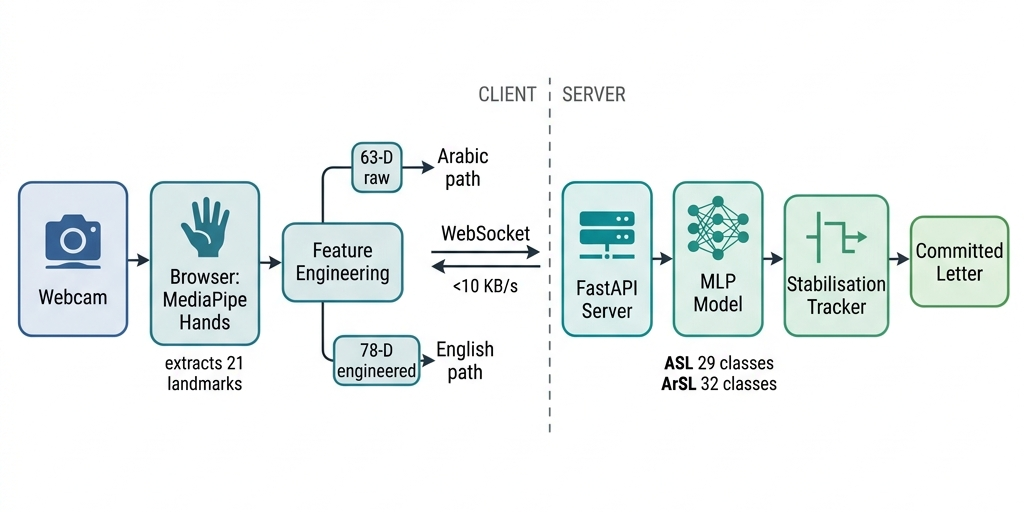
\includegraphics[width=0.90\textwidth]{images/fig_3-3_letter_pipeline.png}
\caption{Letter-mode client--server pipeline. The browser captures a webcam frame as a base64-encoded JPEG and sends it via HTTP \texttt{POST} to the Node.js application tier; the gateway proxies the request to FastAPI, where MediaPipe Hands extracts landmarks and engineers a 63-D (ArSL) or 78-D (ASL) vector before the letter MLP and stabilisation decoder commit a character.}
\label{fig:ch3-letter-pipeline}
\end{figure}
\vspace{0.6cm}
\clearpage
% --- 3.2 DATASETS ---
\noindent\textbf{3.2\quad LETTER DATASETS AND SPLIT POLICIES}\par
\addcontentsline{toc}{section}{\numberline{3.2}LETTER DATASETS AND SPLIT POLICIES}
\vspace{0.4cm}

\noindent The following table summarises the two letter corpora. Static images use random stratified splits~\cite{akash2019aslalphabet,arthur2018arasl2018}.\par\vspace{0.4cm}

\begin{table}[H]
\centering
\caption{Letter datasets, feature shapes, and split policies.}
\label{tab:ch3-letter-datasets}
\small
\begin{tabular}{|P{1.5cm}|P{2.2cm}|c|c|c|P{2.8cm}|}
\hline
\textbf{Task} & \textbf{Dataset} & \textbf{Classes} & \textbf{Features} & \textbf{Frames} & \textbf{Split} \\
\hline
ASL letters & ASL Alphabet & 29 (28 deploy.) & 78-D & 1 & $\sim$64/16/20 train/val/test \\
ArSL letters & ArASL2018 & 32 & 63-D & 1 & 60/20/20 train/val/test \\
\hline
\end{tabular}
\end{table}
\vspace{0.4cm}

\noindent\textbf{Training software environment.} Letter and word training share a common Python stack (as defined in Table~\ref{tab:ch3-env}). Heavy jobs --- Holistic extraction over KArSL videos and Inception I3D fine-tuning experiments --- were run on \textbf{Kaggle GPU} (T4/P100/L4, CUDA~11.x) when local VRAM was insufficient; letter MLP training and live prototyping used a \textbf{4\,GB NVIDIA GPU} on the development laptop. TensorFlow/Keras letter and ArSL word training enable GPU memory growth; PyTorch loads the ASL I3D checkpoint for server inference~\cite{abadi2016tensorflow,chollet2015keras,kingma2015adam}.\par\vspace{0.3cm}

\begin{table}[H]
\centering
\caption{Training and inference software environment (letters and words).}
\label{tab:ch3-env}
\small
\begin{tabular}{|l|l|}
\hline
\textbf{Component} & \textbf{Version / role} \\
\hline
Python & 3.9+ \\
TensorFlow / Keras~\cite{abadi2016tensorflow,chollet2015keras} & 2.x --- letter MLPs, ArSL word BiLSTM \\
PyTorch~\cite{pytorch2024} & 2.x --- ASL word Inception I3D (\texttt{asl\_word\_i3d.pt}) \\
CUDA / cuDNN~\cite{chetlur2014cudnn} & 11.x (Kaggle GPU; local 4\,GB GPU when available) \\
MediaPipe~\cite{zhang2020mediapipe,mediapipeweb} & 0.10.x (Python extraction; JS/WASM in browser) \\
OpenCV, NumPy, scikit-learn~\cite{opencv2024docs,harris2020numpy,pedregosa2011sklearn} & Feature I/O, metrics \\
Jupyter~\cite{kluyver2016jupyter} & Interactive training environment \\
Adam optimiser~\cite{kingma2015adam} & $\eta{=}10^{-3}$ default (letters); word schedules in Ch.~4 \\
\hline
\end{tabular}
\end{table}
\vspace{0.3cm}
\clearpage
\noindent\textbf{3.2.1\quad ASL Alphabet (English Letters):}\par
\addcontentsline{toc}{subsection}{\numberline{3.2.1}ASL Alphabet (English Letters):}
\vspace{0.3cm}
\noindent The Kaggle ASL Alphabet corpus provides $\sim$87\,000 static hand images across 29 classes (A--Z plus \texttt{space}, \texttt{del}, \texttt{nothing})~\cite{akash2019aslalphabet}. The graduation \textbf{deployed} ASL letter model excludes the \texttt{nothing} control class, yielding a 28-way label space (Chapter~6). Images are converted \textbf{offline} to MediaPipe Hand landmarks, then augmented with wrist-relative normalisation and 15 inter-joint angles to form a 78-D engineered vector cached in CSV/NPZ before MLP training. The \textbf{same} 78-D representation is computed in the browser at inference time, eliminating train/serve skew on input geometry~\cite{zhang2020mediapipe}.\par\vspace{0.4cm}

\noindent\textbf{3.2.2\quad ArASL2018 (Arabic Letters):}\par
\addcontentsline{toc}{subsection}{\numberline{3.2.2}ArASL2018 (Arabic Letters):}
\vspace{0.3cm}

\noindent ArASL2018 provides 54\,049 images across 32 Arabic finger-spelling classes~\cite{arthur2018arasl2018}. Processing mirrors the landmark extraction stage of the ASL pipeline but uses the flattened 63-D raw coordinate vector without additional angle features. Visually similar letter pairs (e.g.\ \arTxt{ك}/\arTxt{ل}) motivate per-class evaluation in Chapter~6. Model~2 shares the same \textbf{MLP family} as Model~1 (Dense--BN--ReLU--Dropout blocks) but uses a \textbf{wider, separately trained head} with different input dimension, hidden widths, and hyperparameters (Section~3.5; Table~\ref{tab:ch3-arch-compare}).\par\vspace{0.4cm}

\noindent\textbf{3.2.3\quad End-to-End Training Pipeline (Dataset to \texttt{.h5} Artifact):}\par
\addcontentsline{toc}{subsection}{\numberline{3.2.3}End-to-End Training Pipeline:}
\vspace{0.3cm}

\noindent Both letter corpora follow the same offline preparation and training pipeline. The numbered steps below trace the complete path from raw image dataset to the exported checkpoint used by the FastAPI inference service.

\begin{enumerate}

\item \textbf{Image loading.} Dataset images are read from disk (JPEG/PNG) and converted to RGB. MediaPipe Hands is initialised with \texttt{static\_image\_mode=True}, \texttt{max\_num\_hands=1}, and \texttt{min\_detection\_confidence=0.7}. Unreadable or empty files are skipped.

\item \textbf{Landmark extraction.} For each image, MediaPipe returns 21 hand landmarks $\{(x_i, y_i, z_i)\}_{i=0}^{20}$ normalised to image coordinates $[0,1]^2$ with depth estimate $z_i$. Images where no hand is detected are discarded. Detection rates are approximately 69\,\% for ASL Alphabet and 77\,\% for ArASL2018, yielding $\sim$60\,k and $\sim$74\,k successful samples respectively.

\item \textbf{Feature engineering.} Extracted landmarks are transformed into a fixed-length feature vector (see Section~3.3):
\[
\mathbf{x} = \begin{cases} \mathbf{x}_{\text{raw}} \in \mathbb{R}^{63} & \text{ArSL: flatten } (x_i, y_i, z_i)^\top \text{ directly,} \\ \mathbf{x}_{\text{ASL}} \in \mathbb{R}^{78} & \text{ASL: wrist-centred 21 landmarks + 15 angles ($63{+}15$).}\end{cases}
\]

\item \textbf{Caching.} Feature vectors and class labels are written to a CSV file (\texttt{asl\_letters\_engineered.csv} / \texttt{ASLAD-3000\_v2.csv}) and a compressed NPZ archive for fast NumPy loading. This step runs once; subsequent training passes load directly from cache.

\item \textbf{Train / validation / test split.} The feature matrix $X \in \mathbb{R}^{N \times d}$ is split with \textbf{stratified} sampling (preserving per-class proportions) using \texttt{random\_state=42}:
\begin{equation}
\label{eq:ch3-split}
(X_{\text{train}},\, X_{\text{val}},\, X_{\text{test}}) \quad \text{proportions } \begin{cases} 0.64 : 0.16 : 0.20 & \text{(ASL)} \\ 0.60 : 0.20 : 0.20 & \text{(ArSL)} \end{cases}
\end{equation}
Test split is isolated before any hyperparameter search and is touched exactly once for final reporting.

\item \textbf{One-hot label encoding.} Integer class indices are converted to one-hot vectors:
\begin{equation}
\label{eq:ch3-onehot}
\mathbf{y} = \mathbf{e}_c \in \{0,1\}^C, \qquad e_{c,k} = \mathbb{1}[k = c], \qquad C \in \{28,\,32\},
\end{equation}
via Keras \texttt{to\_categorical} (or \texttt{np.eye} for ArSL when TensorFlow is loaded later in the pipeline). Feature vectors are fed \textbf{directly} to the MLP without an external \texttt{StandardScaler}; batch normalisation inside the network handles activation scaling during training. (Deployed word models likewise use no external scaler at inference; see Chapter~4.)

\item \textbf{Model construction.} The MLP is assembled with the Keras \texttt{Sequential} API. Layer widths, BN placement, dropout rates, and output softmax dimension are specified per model (Sections~3.4 and~3.5; Figure~\ref{fig:ch3-mlp-heads}).

\item \textbf{Callbacks.} Three callbacks are registered before \texttt{model.fit}:
\begin{itemize}
  \item \textbf{ModelCheckpoint}~\cite{chollet2015keras}: saves the \texttt{.h5} artifact to disk whenever \texttt{val\_accuracy} improves (\texttt{save\_best\_only=True}, \texttt{mode='max'}).
  \item \textbf{EarlyStopping}~\cite{chollet2015keras}: monitors \texttt{val\_loss}; halts training when no improvement is seen for \texttt{patience} consecutive epochs and restores the best weights (\texttt{restore\_best\_weights=True}).
  \item \textbf{ReduceLROnPlateau} (ArSL only)~\cite{chollet2015keras}: multiplies the current learning rate by factor 0.5 when \texttt{val\_loss} does not improve for 7 consecutive epochs, floored at $\eta_{\min} = 10^{-7}$.
\end{itemize}

\item \textbf{Mini-batch training.} Parameters $\theta$ are updated over mini-batches of size $B \in \{64,\,256\}$ using the Adam optimiser. At each step $t$ with gradient $g_t = \nabla_\theta \mathcal{L}$:
\begin{align}
m_t &= \beta_1 m_{t-1} + (1-\beta_1)\, g_t, \label{eq:adam-m}\\
v_t &= \beta_2 v_{t-1} + (1-\beta_2)\, g_t^2, \label{eq:adam-v}\\
\hat{m}_t &= \frac{m_t}{1-\beta_1^t}, \qquad \hat{v}_t = \frac{v_t}{1-\beta_2^t}, \label{eq:adam-bias}\\
\theta_t &\leftarrow \theta_{t-1} - \eta\,\frac{\hat{m}_t}{\sqrt{\hat{v}_t}+\varepsilon_A}, \label{eq:adam-update}
\end{align}
with defaults $\beta_1{=}0.9$, $\beta_2{=}0.999$, $\varepsilon_A{=}10^{-7}$~\cite{kingma2015adam}.

\item \textbf{Test evaluation.} After training, the best checkpoint is loaded and evaluated \textbf{once} on the held-out test split. Top-1 accuracy, test loss, and a per-class classification report (precision, recall, F1) are recorded for Chapter~6.

\item \textbf{Artifact export.} The best \texttt{.h5} checkpoint is the final deliverable:
\begin{itemize}
  \item ASL: \texttt{asl\_mediapipe\_mlp\_model\_engineered.h5}
  \item ArSL: \texttt{arsl\_mediapipe\_mlp\_model\_bestV2.2.h5}
\end{itemize}
The FastAPI inference service loads these at startup (Chapter~5); no further post-processing (quantisation, pruning) is applied within graduation scope.

\end{enumerate}
\vspace{0.4cm}

\noindent The complete workflow is illustrated in the following figure after the feature definitions in Section~3.3.\par\vspace{0.4cm}

% --- 3.3 FEATURES ---
\noindent\textbf{3.3\quad FEATURE EXTRACTION FOR LETTERS}\par
\addcontentsline{toc}{section}{\numberline{3.3}FEATURE EXTRACTION FOR LETTERS}
\vspace{0.4cm}

\noindent MediaPipe Hands outputs 21 $(x,y,z)$ points per hand~\cite{zhang2020mediapipe}. For finger-spelling, \texttt{max\_num\_hands=1} suffices; face and pose modules are reserved for word models (Chapter~4). Missing landmarks are zero-filled; the live client mirrors training conventions. As shown in Figure~\ref{fig:ch3-landmarks}, the diagram labels the wrist (0) and the four finger chains (thumb 1--4, index 5--8, middle 9--12, ring 13--16, pinky 17--20).\par\vspace{0.4cm}

\begin{figure}[H]
\centering
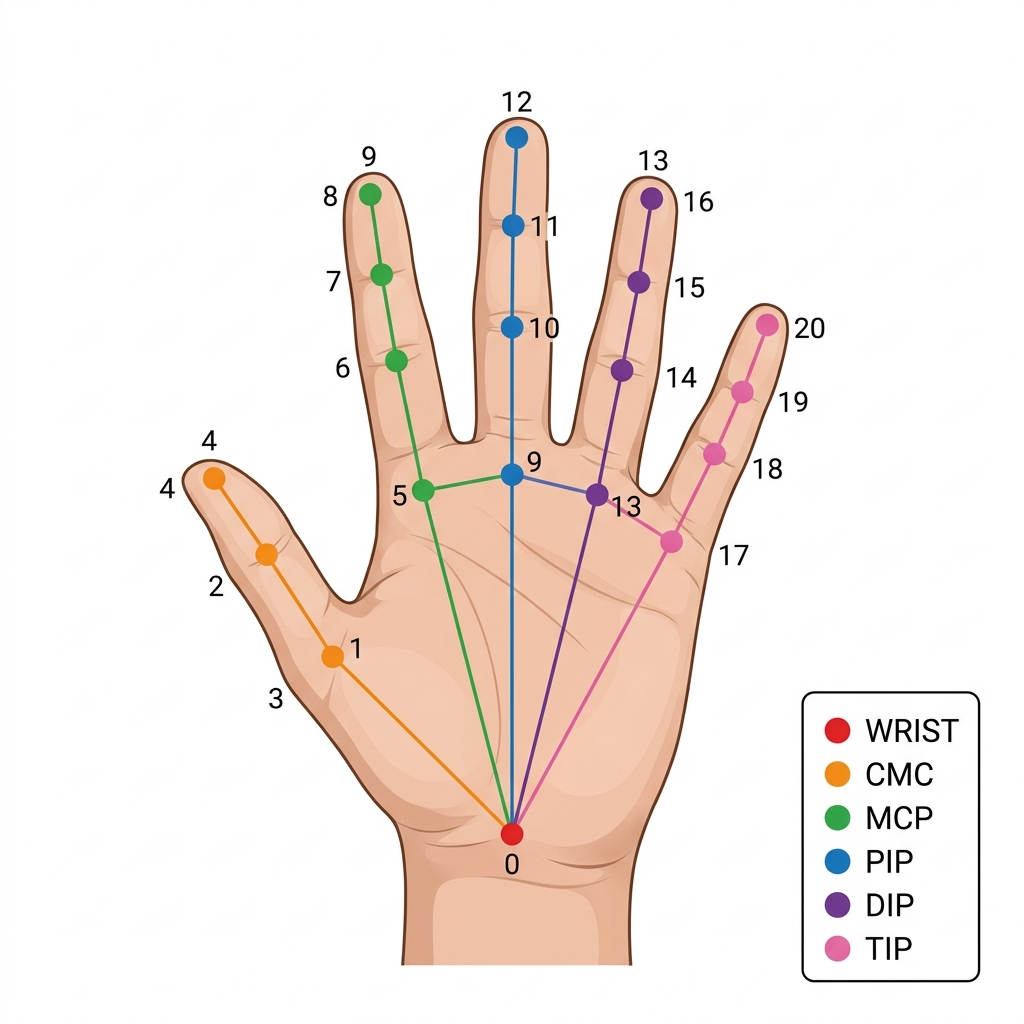
\includegraphics[width=0.9\textwidth]{images/fig_3-1_mediapipe_landmarks.png}
\caption{MediaPipe Hand landmark topology (21 points). Each landmark contributes $(x,y,z)$ coordinates; flattening yields a 63-D raw vector.}
\label{fig:ch3-landmarks}
\end{figure}
\vspace{0.4cm}

\begin{figure}[H]
\centering
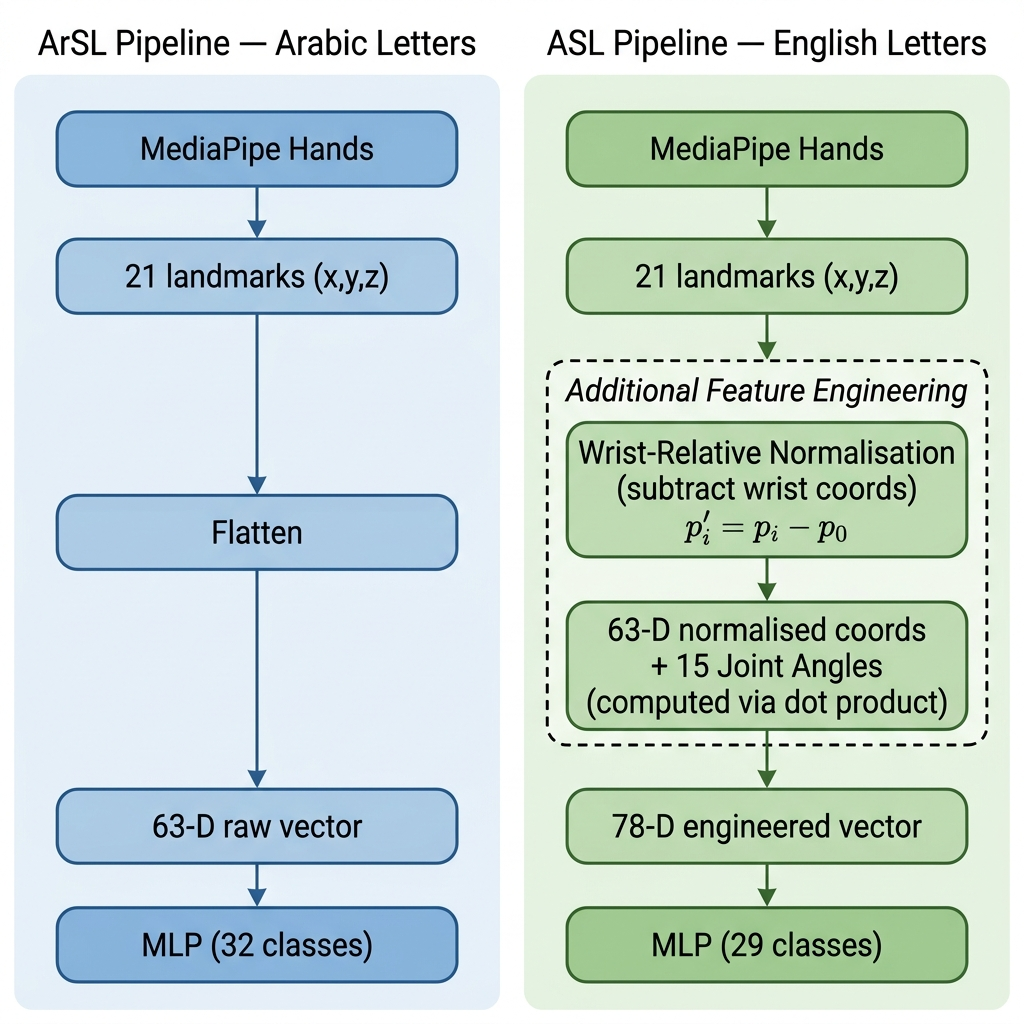
\includegraphics[width=0.88\textwidth]{images/fig_3-5_feature_engineering.png}
\caption{Letter feature-engineering split. ArSL (left): MediaPipe Hands $\rightarrow$ flatten $\rightarrow$ 63-D raw MLP (32 classes). ASL (right): additional wrist-relative normalisation and 15 joint angles $\rightarrow$ 78-D engineered MLP (28 deployed classes).}
\label{fig:ch3-feature-eng}
\end{figure}
\vspace{0.4cm}

\noindent The two letter pipelines diverge after landmark extraction (as illustrated in Figure~\ref{fig:ch3-feature-eng}). Let $\mathbf{p}_i = (x_i, y_i, z_i)^\top \in \mathbb{R}^3$ denote landmark $i$ with wrist index $i{=}0$. The raw feature vector is
\begin{equation}
\label{eq:ch3-x-raw}
\mathbf{x}_{\text{raw}} = \bigl[x_0, y_0, z_0, x_1, y_1, z_1, \ldots, x_{20}, y_{20}, z_{20}\bigr]^\top \in \mathbb{R}^{63}.
\end{equation}
\textbf{ArSL (Model~2)} uses $\mathbf{x}_{\text{raw}}$ directly. \textbf{ASL (Model~1)} wrist-centres every landmark and appends 15 inter-joint angles:
\begin{equation}
\mathbf{p}'_i = \mathbf{p}_i - \mathbf{p}_0, \qquad i = 0,\ldots,20,
\end{equation}
\begin{equation}
\theta_j = \arccos\!\left(\frac{\mathbf{v}_{j,1} \cdot \mathbf{v}_{j,2}}{\|\mathbf{v}_{j,1}\|\,\|\mathbf{v}_{j,2}\| + \epsilon}\right), \qquad j = 1,\ldots,15,
\end{equation}
where $\mathbf{v}_{j,1} = \mathbf{p}'_{a_j} - \mathbf{p}'_{b_j}$ and $\mathbf{v}_{j,2} = \mathbf{p}'_{c_j} - \mathbf{p}'_{b_j}$ are the two bone vectors meeting at joint $b_j$ (the middle landmark of the triplet $(a_j, b_j, c_j)$), and $\epsilon{=}10^{-8}$ avoids division by zero. The 15 triplets cover three joints per finger (metacarpo-phalangeal MCP, proximal inter-phalangeal PIP, distal inter-phalangeal DIP) across all five fingers, as defined in Table~\ref{tab:ch3-angle-triplets}. The deployed ASL input concatenates all wrist-centred coordinates with the angle block:
\begin{equation}
\label{eq:ch3-x-asl}
\mathbf{x}_{\text{ASL}} = \bigl[\,\mathbf{p}'_0, \ldots, \mathbf{p}'_{20};\; \theta_1, \ldots, \theta_{15}\,\bigr]^\top \in \mathbb{R}^{78},
\end{equation}
i.e.\ $21 \times 3 = 63$ translation-invariant landmark values (with $\mathbf{p}'_0 \equiv \mathbf{0}$) plus 15 scalar angles. The same 78-D layout is reproduced in the browser at inference time~\cite{zhang2020mediapipe}.

\begin{table}[H]
\centering
\caption{The 15 inter-joint angle triplets used in the 78-D ASL feature vector. Each row specifies the landmark index triple $(a, b, c)$ where $b$ is the vertex joint; the angle is computed between bone vectors $b{\to}a$ and $b{\to}c$.}
\label{tab:ch3-angle-triplets}
\small
\begin{tabular}{|l|c|c|}
\hline
\textbf{Finger} & \textbf{Joint} & \textbf{Triplet $(a, b, c)$} \\
\hline
Thumb  & MCP & (0, 1, 2) \\
Thumb  & PIP & (1, 2, 3) \\
Thumb  & DIP & (2, 3, 4) \\
Index  & MCP & (0, 5, 6) \\
Index  & PIP & (5, 6, 7) \\
Index  & DIP & (6, 7, 8) \\
Middle & MCP & (0, 9, 10) \\
Middle & PIP & (9, 10, 11) \\
Middle & DIP & (10, 11, 12) \\
Ring   & MCP & (0, 13, 14) \\
Ring   & PIP & (13, 14, 15) \\
Ring   & DIP & (14, 15, 16) \\
Pinky  & MCP & (0, 17, 18) \\
Pinky  & PIP & (17, 18, 19) \\
Pinky  & DIP & (18, 19, 20) \\
\hline
\end{tabular}
\end{table}
\vspace{0.4cm}

\noindent The following table summarises the complete feature-vector composition for each letter model, cross-referencing dimensions to the equations above.

\begin{table}[H]
\centering
\caption{Feature-vector dimension breakdown for the two letter models.}
\label{tab:ch3-feature-dim}
\small
\begin{tabular}{|P{2.4cm}|r|P{3.6cm}|P{3.6cm}|}
\hline
\textbf{Component} & \textbf{Dims} & \textbf{ASL (Model~1)} & \textbf{ArSL (Model~2)} \\
\hline
Wrist-centred coords $\mathbf{p}'_{0\ldots20}$ & 63 & Yes (Eq.~\eqref{eq:ch3-x-asl}) & No (raw wrist incl.) \\
Raw wrist $(x_0,y_0,z_0)$                        &  3 & (included in $\mathbf{p}'_0{=}\mathbf{0}$) & Yes \\
Raw landmarks $\mathbf{p}_{1\ldots20}$           & 60 & No  & Yes \\
Joint angles $\theta_{1\ldots15}$                & 15 & Yes (Table~\ref{tab:ch3-angle-triplets}) & No \\
\hline
\textbf{Total}                                   & \textbf{78} / \textbf{63} & \textbf{78-D} & \textbf{63-D} \\
\hline
\end{tabular}
\end{table}
\vspace{0.4cm}

\noindent Holistic/Pose+Hands extensions for word models are summarised as set out in Table~\ref{tab:feature-vectors} (Chapter~2).\par\vspace{0.4cm}

\noindent As summarised in Figure~\ref{fig:ch3-training-pipeline}, the offline training path runs from dataset images to the exported \texttt{.h5} checkpoint. Shared stages (landmark extraction through label encoding) are identical for both languages; ASL and ArSL diverge at feature engineering and at MLP head configuration (as compared in Figure~\ref{fig:ch3-mlp-heads} and Table~\ref{tab:ch3-arch-compare}).

\begin{figure}[H]
\centering
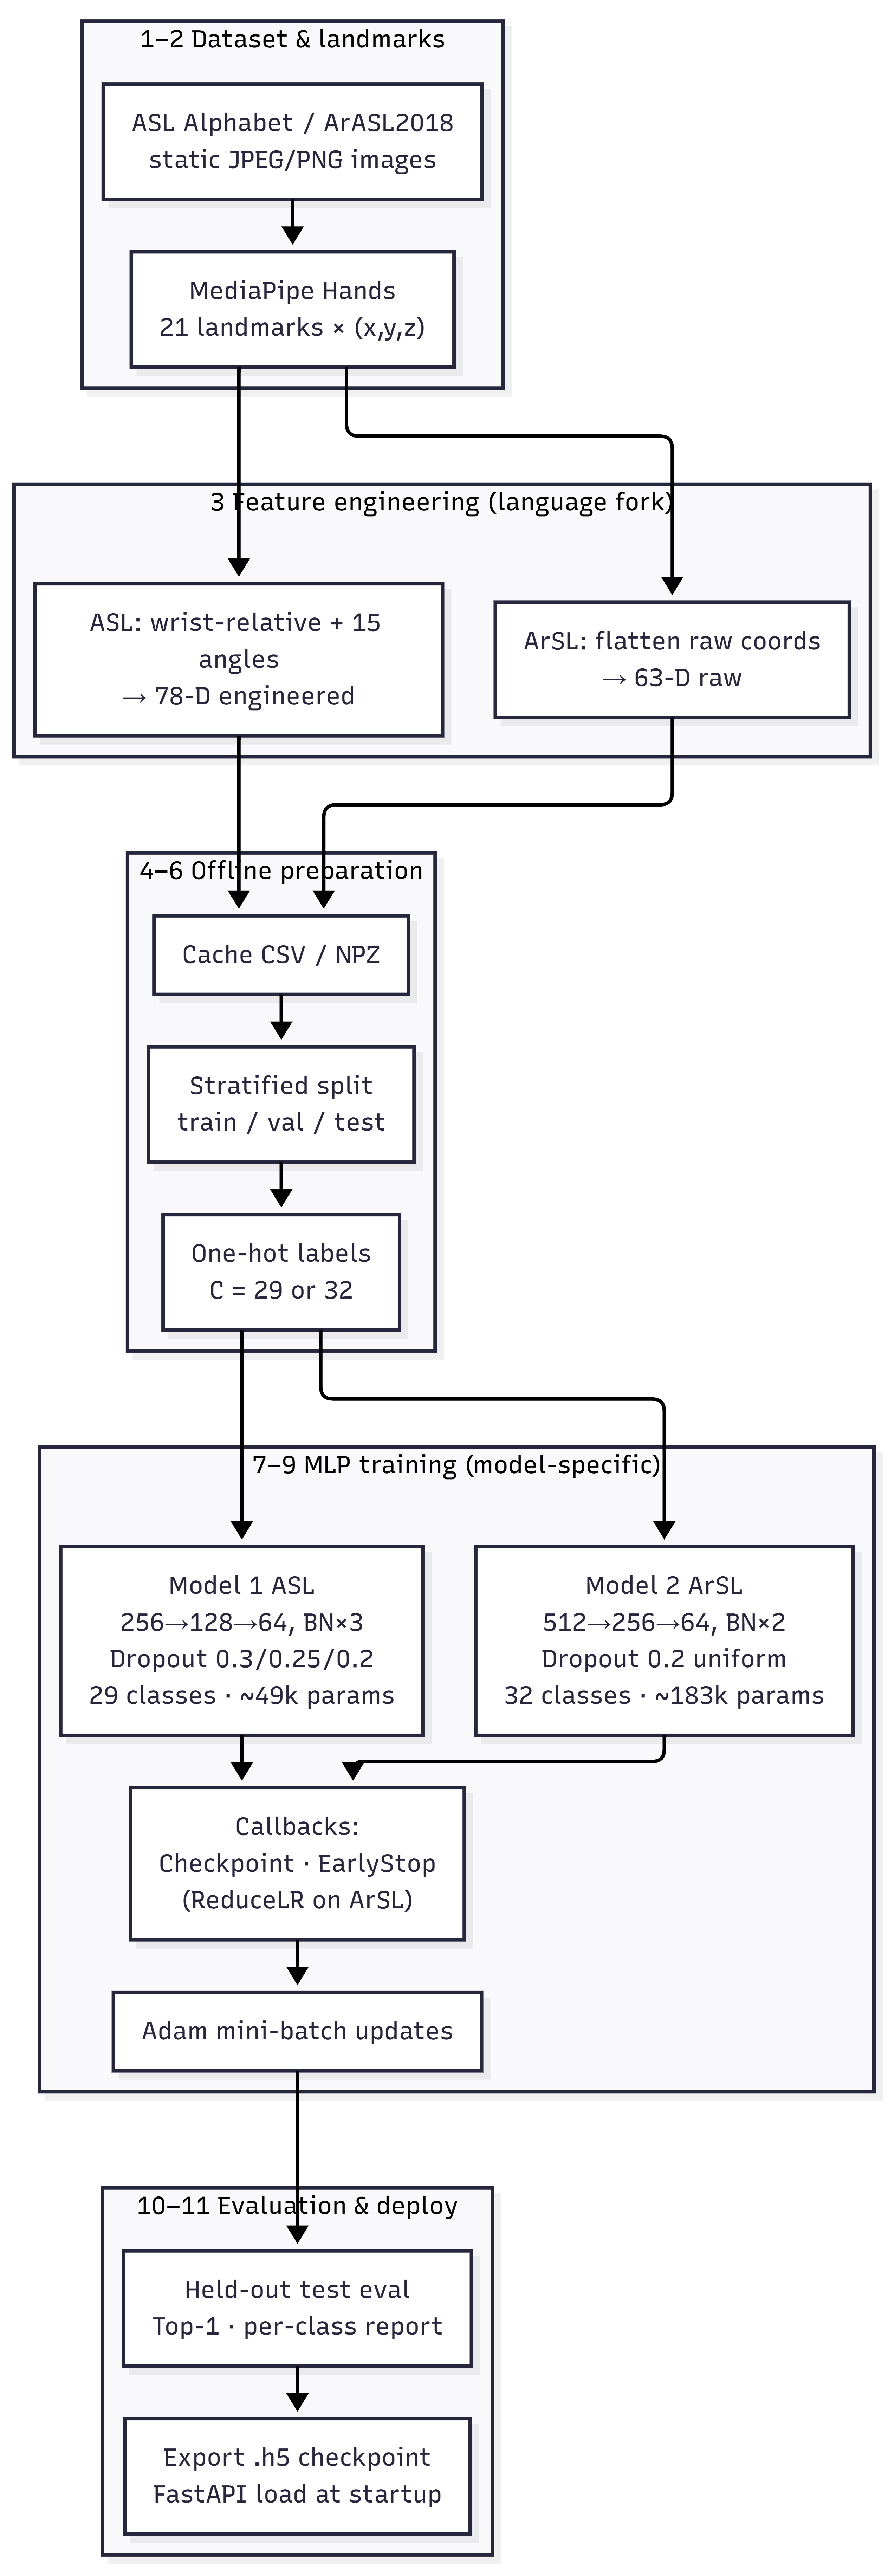
\includegraphics[width=0.90\textwidth,height=0.95\textheight,keepaspectratio]{images/fig_3-8_letter_training_pipeline.png}
\caption{End-to-end letter training pipeline. Stages~1--6 are shared; language-specific forks appear at feature engineering (78-D engineered vs.\ 63-D raw) and at MLP head width, dropout, and training schedule.}
\label{fig:ch3-training-pipeline}
\end{figure}
\vspace{0.6cm}

% --- 3.4 MODEL 1 ---
\noindent\textbf{3.4\quad MODEL 1 --- ASL LETTER MLP}\par
\addcontentsline{toc}{section}{\numberline{3.4}MODEL 1 --- ASL LETTER MLP}
\vspace{0.15cm} % Cramped from 0.4cm

\noindent\textbf{Problem:} finger-spelled ASL letters are quasi-static poses; one frame suffices~\cite{akash2019aslalphabet}.\par\vspace{0.15cm} % Cramped from 0.3cm

\noindent\textbf{Input and notation.} Each training or inference sample is a single engineered vector $\mathbf{x} \in \mathbb{R}^{78}$ from Equation~\eqref{eq:ch3-x-asl}. The model implements a three-hidden-layer MLP with batch normalisation, ReLU, dropout, and softmax (Figures~\ref{fig:ch3-mlp} and~\ref{fig:ch3-mlp-heads}). Layer widths are $d_0{=}78$, $d_1{=}256$, $d_2{=}128$, $d_3{=}64$, and output dimension $C{=}28$ (A--Z, \texttt{space}, \texttt{del}).\par\vspace{0.15cm} % Cramped from 0.3cm

% --- MATH SPACING OVERRIDE ---
% This block temporarily shrinks the massive empty spaces LaTeX puts around equations
\begingroup
\setlength{\abovedisplayskip}{3pt}
\setlength{\belowdisplayskip}{3pt}
\setlength{\abovedisplayshortskip}{3pt}
\setlength{\belowdisplayshortskip}{3pt}

\noindent\textbf{Forward pass.} Each hidden block $\ell \in \{1,2,3\}$ applies a dense affine transform, batch normalisation, ReLU, and dropout (Section~2.4.1 summarises the MLP family at a high level). With input $\mathbf{h}^{(0)} = \mathbf{x}$, layer $\ell$ computes
\begin{equation}
\tilde{\mathbf{h}}^{(\ell)} = W^{(\ell)} \mathbf{h}^{(\ell-1)} + \mathbf{b}^{(\ell)}, \qquad \mathbf{h}^{(\ell)} = \mathrm{Dropout}_p\!\Big(\mathrm{ReLU}\big(\mathrm{BN}(\tilde{\mathbf{h}}^{(\ell)})\big)\Big),
\end{equation}
with $\mathbf{h}^{(0)} = \mathbf{x}$. Batch normalisation~\cite{ioffe2015batchnorm} standardises each pre-activation batch dimension:
\begin{equation}
\mathrm{BN}(\tilde{h}) = \gamma \,\frac{\tilde{h} - \mu_B}{\sqrt{\sigma_B^2 + \epsilon}} + \beta,
\end{equation}
where $\mu_B$ and $\sigma_B^2$ are batch mean and variance at training time (running statistics at inference). Dropout~\cite{srivastava2014dropout} zeroes each activation independently with probability $p \in \{0.3, 0.25, 0.2\}$ on layers 1--3 respectively. Class logits $\mathbf{z} \in \mathbb{R}^{28}$ and probabilities follow
\begin{equation}
\mathbf{z} = W^{(4)} \mathbf{h}^{(3)} + \mathbf{b}^{(4)}, \qquad
P(y{=}k \mid \mathbf{x}) = \frac{\exp(z_k)}{\sum_{j=1}^{28} \exp(z_j)}.
\end{equation}
The predicted letter is $\hat{y} = \arg\max_k P(y{=}k \mid \mathbf{x})$.\par\vspace{0.15cm} % Cramped from 0.3cm

\noindent\textbf{Loss and optimisation.} Training minimises categorical cross-entropy over one-hot labels $\mathbf{y}$:
\begin{equation}
\mathcal{L}_{\text{CE}} = -\sum_{k=1}^{28} y_k \log P(y{=}k \mid \mathbf{x}).
\end{equation}
\endgroup % Ends the math spacing override
% -----------------------------

\enlargethispage{\baselineskip} % MAGIC TRICK: Forces this specific page to stretch one line longer at the bottom margin to catch the spilling text

\noindent Parameters are updated with the \textbf{Adam} optimiser~\cite{kingma2015adam} at $\eta{=}10^{-3}$. Adam maintains per-parameter first and second moment estimates $(m_t, v_t)$ with bias-correction; the update at step $t$ is identical in form to Equations~\eqref{eq:adam-m}--\eqref{eq:adam-update} in Section~3.2.3 with $\beta_1{=}0.9$, $\beta_2{=}0.999$, $\varepsilon_A{=}10^{-7}$. \textbf{EarlyStopping} halts training when \texttt{val\_loss} fails to decrease for \textbf{patience~=~5} consecutive epochs; \texttt{restore\_best\_weights=True} reloads the checkpoint that achieved the lowest validation loss. Maximum training duration is 20 epochs; ModelCheckpoint saves the best \texttt{val\_accuracy} snapshot as the exported artifact.\par\vspace{0.2cm} % Cramped from 0.3cm

\clearpage

\noindent\textbf{Parameter count.} The trainable weight count is approximately
\begingroup
\setlength{\abovedisplayskip}{3pt}
\setlength{\belowdisplayskip}{3pt}
\begin{equation}
|\theta| \approx \underbrace{78{\times}256 + 256}_{\text{layer 1}} + \underbrace{256{\times}128 + 128}_{\text{layer 2}} + \underbrace{128{\times}64 + 64}_{\text{layer 3}} + \underbrace{64{\times}28 + 28}_{\text{softmax}} \approx 49\text{k},
\end{equation}
\endgroup
excluding batch-norm scale/shift terms ($\sim$1.8\,k additional). This footprint supports sub-50\,ms single-frame inference on laptop CPU/GPU~\cite{zhang2020mediapipe}.\par\vspace{0.2cm} % Cramped from 0.3cm

\noindent\textbf{Training setup.} Batch size 256 (GPU) or 64 (CPU); exported artifact \texttt{asl\_\allowbreak mediapipe\_\allowbreak mlp\_\allowbreak model\_\allowbreak engineered.h5}.\par\vspace{0.3cm} % Cramped from 0.4cm

\begin{figure}[H]
\centering
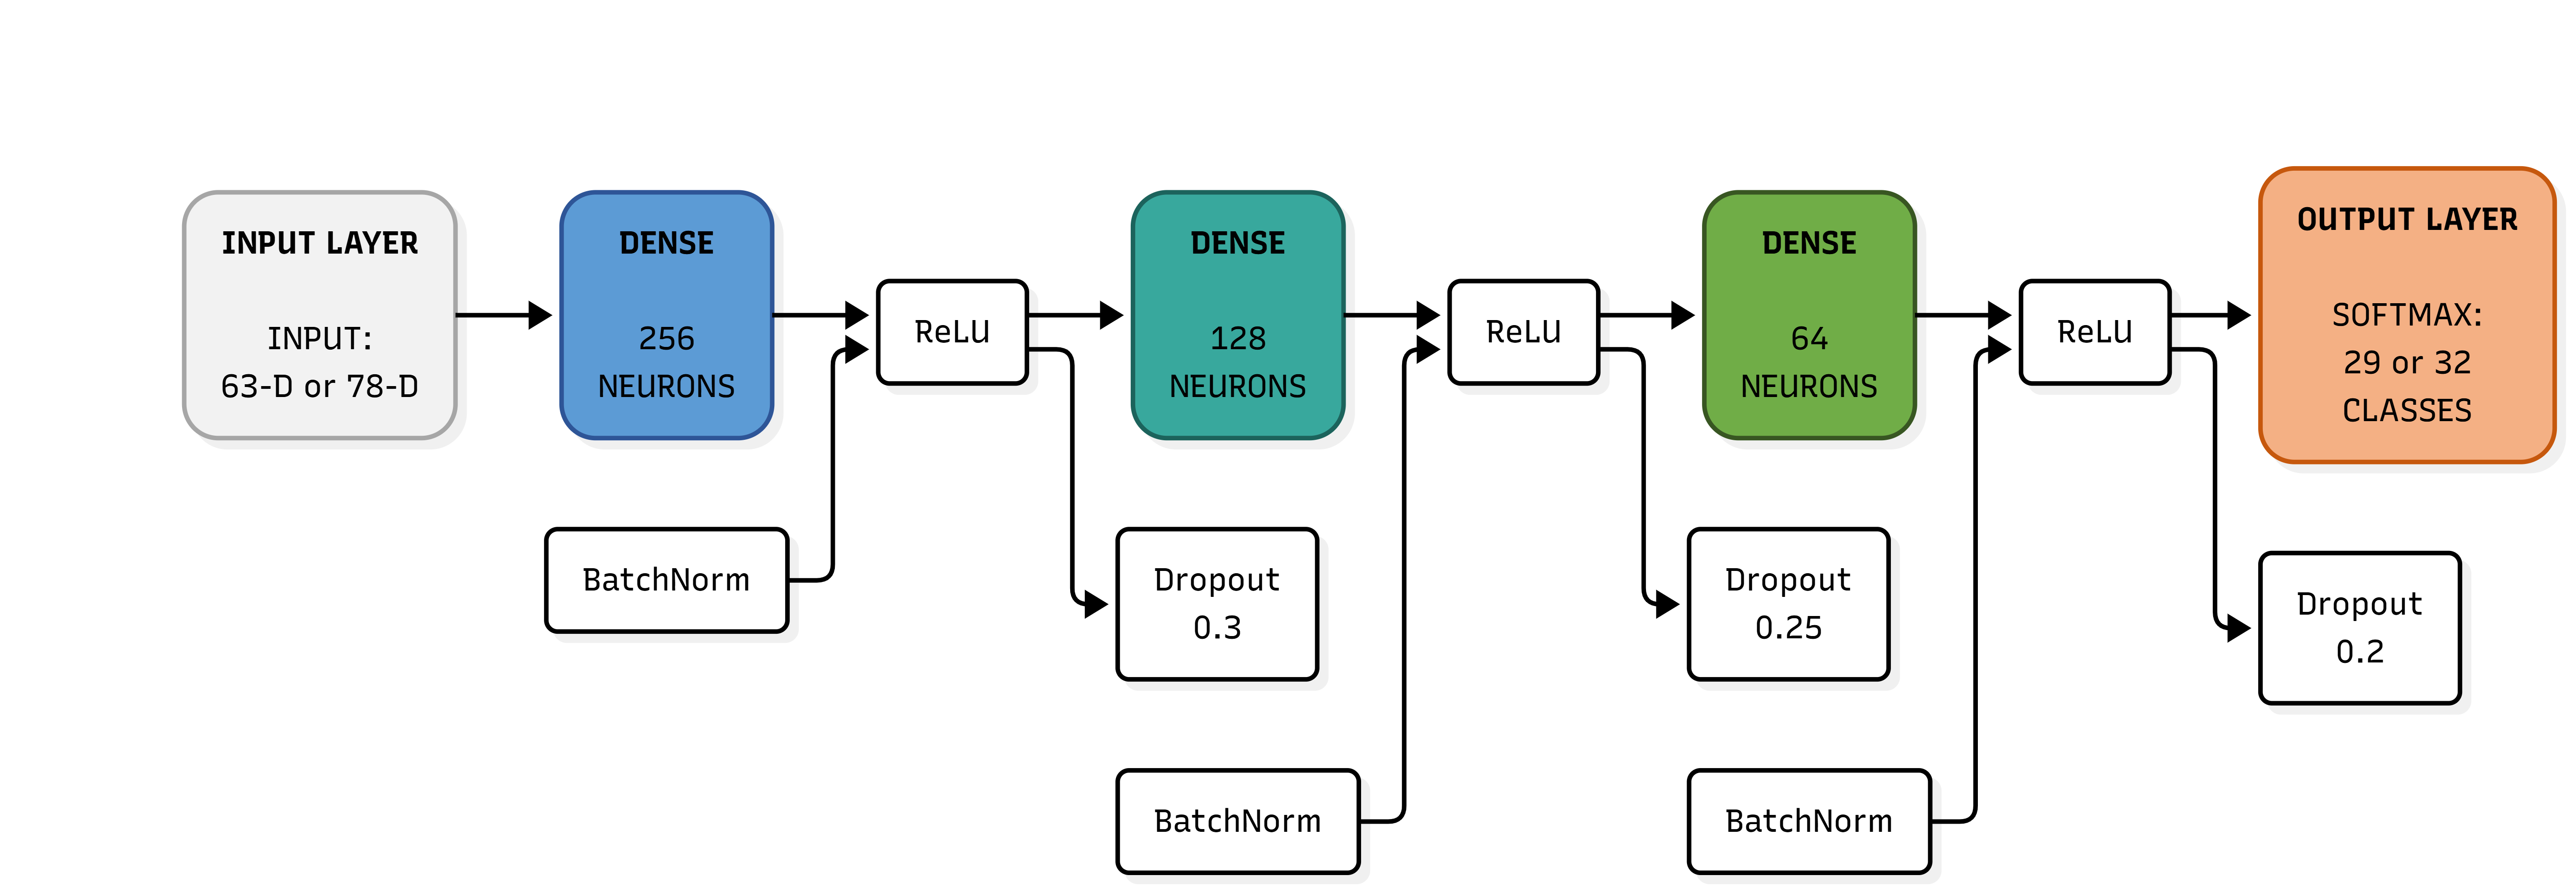
\includegraphics[width=0.9\textwidth]{images/fig_3-2_mlp_architecture.png}
\caption{Shared MLP \emph{family} for both letter models (Dense--BN--ReLU--Dropout--Softmax). ASL Model~1 uses 78-D input, widths 256/128/64, BN on all three hidden layers, and progressive dropout (0.3 / 0.25 / 0.2). ArSL Model~2 uses 63-D input, wider layers 512/256/64, BN on layers~1--2 only, and uniform dropout 0.2 (Table~\ref{tab:ch3-arch-compare}).}
\label{fig:ch3-mlp}
\end{figure}
\vspace{0.4cm} % Cramped from 0.6cm

% --- 3.5 MODEL 2 ---
\noindent\textbf{3.5\quad MODEL 2 --- ArSL LETTER MLP}\par
\addcontentsline{toc}{section}{\numberline{3.5}MODEL 2 --- ArSL LETTER MLP}
\vspace{0.4cm}

\noindent Model~2 shares the same \textbf{MLP family} as Model~1 but uses a wider architecture tuned on the ArSL corpus: input $\mathbf{x} \in \mathbb{R}^{63}$ equals $\mathbf{x}_{\text{raw}}$ from Equation~\eqref{eq:ch3-x-raw}; hidden widths are $d_1{=}512$, $d_2{=}256$, $d_3{=}64$ with uniform dropout $p{=}0.2$ on all three layers and batch normalisation after dense layers 1 and 2 only.\par\vspace{0.3cm}

\noindent\textbf{Forward pass.} Substituting $d_0{=}63$ into the Model~1 recurrence,
\begin{equation}
\mathbf{h}^{(0)} = \mathbf{x}_{\text{raw}}, \qquad
\tilde{\mathbf{h}}^{(\ell)} = W^{(\ell)} \mathbf{h}^{(\ell-1)} + \mathbf{b}^{(\ell)}, \quad \ell \in \{1,2,3\},
\end{equation}
with $W^{(1)} \in \mathbb{R}^{512 \times 63}$, $W^{(2)} \in \mathbb{R}^{256 \times 512}$, $W^{(3)} \in \mathbb{R}^{64 \times 256}$, and output weights $W^{(4)} \in \mathbb{R}^{32 \times 64}$. BN--ReLU--Dropout is applied after layers~1 and~2; layer~3 uses ReLU--Dropout (no BN). Class logits and probabilities are
\begin{equation}
\mathbf{z} = W^{(4)} \mathbf{h}^{(3)} + \mathbf{b}^{(4)}, \qquad
P(y{=}k \mid \mathbf{x}) = \frac{\exp(z_k)}{\sum_{j=1}^{32} \exp(z_j)}, \qquad \hat{y} = \arg\max_k P(y{=}k \mid \mathbf{x}).
\end{equation}
Training minimises the 32-way cross-entropy $\mathcal{L}_{\text{CE}} = -\sum_{k=1}^{32} y_k \log P(y{=}k \mid \mathbf{x})$ with Adam at $\eta_0{=}5\times10^{-4}$ (Equations~\eqref{eq:adam-m}--\eqref{eq:adam-update}). EarlyStopping monitors \texttt{val\_loss} with patience~15 and \texttt{restore\_best\_weights=True}; maximum epochs~100. ReduceLROnPlateau applies the schedule
\begin{equation}
\label{eq:rlrop}
\eta \leftarrow \max\!\bigl(\eta \times 0.5,\; \eta_{\min}\bigr), \qquad \eta_{\min} = 10^{-7},
\end{equation}
whenever \texttt{val\_loss} does not decrease for 7 consecutive epochs~\cite{kingma2015adam}. Mixed-precision training (\texttt{mixed\_float16}) is enabled on GPU, reducing memory by $\sim$50\,\%; the output dense layer is cast to \texttt{float32} to preserve softmax numerical stability.\par\vspace{0.3cm}

\noindent\textbf{Parameter count.} With $d_0{=}63$, $d_1{=}512$, $d_2{=}256$, $d_3{=}64$, and $C{=}32$,
\begin{equation}
|\theta| \approx \underbrace{63{\times}512 + 512}_{\text{layer 1}} + \underbrace{512{\times}256 + 256}_{\text{layer 2}} + \underbrace{256{\times}64 + 64}_{\text{layer 3}} + \underbrace{64{\times}32 + 32}_{\text{softmax}} \approx 183\text{k},
\end{equation}
excluding batch-norm scale/shift terms ($\sim$1.5\,k). Model~2 is wider than Model~1 to compensate for the higher intra-class variation and visually similar letter pairs in the ArSL corpus. \textbf{No weight sharing} with Model~1 --- ASL and ArSL finger-spelling use disjoint vocabularies and feature spaces~\cite{arthur2018arasl2018}. Raw coordinates suffice for ArASL2018 because wrist position is already consistent in the studio-captured corpus; ASL benefits from explicit translation and angle invariance on the noisier Kaggle webcam-style images~\cite{akash2019aslalphabet}. Exported artifact: \texttt{arsl\_mediapipe\_mlp\_model\_bestV2.2.h5}. Visually similar Arabic letter pairs (e.g.\ \arTxt{ك}/\arTxt{ل}) motivate separate per-class evaluation in Chapter~6.\par\vspace{0.4cm}

\noindent The following table summarises how the two letter models relate: they share the same \emph{architectural family} (stacked Dense--BN--ReLU--Dropout MLP) and the same offline training pipeline (as summarised in Figure~\ref{fig:ch3-training-pipeline}), but they are \textbf{not identical} --- each has its own input dimension, hidden widths, regularisation, hyperparameters, and exported checkpoint.

\begin{table}[H]
\centering
\caption{Letter MLP architecture comparison. Both models use the same MLP \emph{family} but separate weights and tuned configurations.}
\label{tab:ch3-arch-compare}
\small % Bumped up the font size
\renewcommand{\arraystretch}{1.4} % Adds vertical padding so the full borders don't look cramped
\begin{tabular}{|P{3.2cm}|P{4.5cm}|P{4.5cm}|}
\hline
\textbf{Property} & \textbf{Model 1 (ASL)} & \textbf{Model 2 (ArSL)} \\ \hline
Input features & 78-D engineered & 63-D raw \\ \hline
Hidden layers & 256 $\rightarrow$ 128 $\rightarrow$ 64 & 512 $\rightarrow$ 256 $\rightarrow$ 64 \\ \hline
Batch normalisation & After all 3 hidden layers & After layers 1--2 only \\ \hline
Dropout & 0.3 / 0.25 / 0.2 & 0.2 (uniform) \\ \hline
Output classes & 28 (deploy) & 32 \\ \hline
Parameters (approx.) & $\sim$49\,k & $\sim$183\,k \\ \hline
Train/val/test split & 64/16/20 & 60/20/20 \\ \hline
Learning rate $\eta_0$ & $10^{-3}$ & $5\times10^{-4}$ \\ \hline
EarlyStopping patience & 5 epochs & 15 epochs \\ \hline
Max epochs & 20 & 100 \\ \hline
ReduceLROnPlateau & No & Yes (factor 0.5) \\ \hline
Training pipeline source & ASL letter training pipeline & ArSL letter training pipeline \\ \hline
Exported artifact & \texttt{asl\_\allowbreak mediapipe\_\allowbreak mlp\_\allowbreak model\_\allowbreak engineered.h5} & \texttt{arsl\_\allowbreak mediapipe\_\allowbreak mlp\_\allowbreak model\_\allowbreak bestV2.2.h5} \\ \hline
Weight sharing & \multicolumn{2}{c|}{None --- independent checkpoints} \\ \hline
\end{tabular}
\end{table}
\vspace{0.4cm}

\begin{figure}[H]
\centering
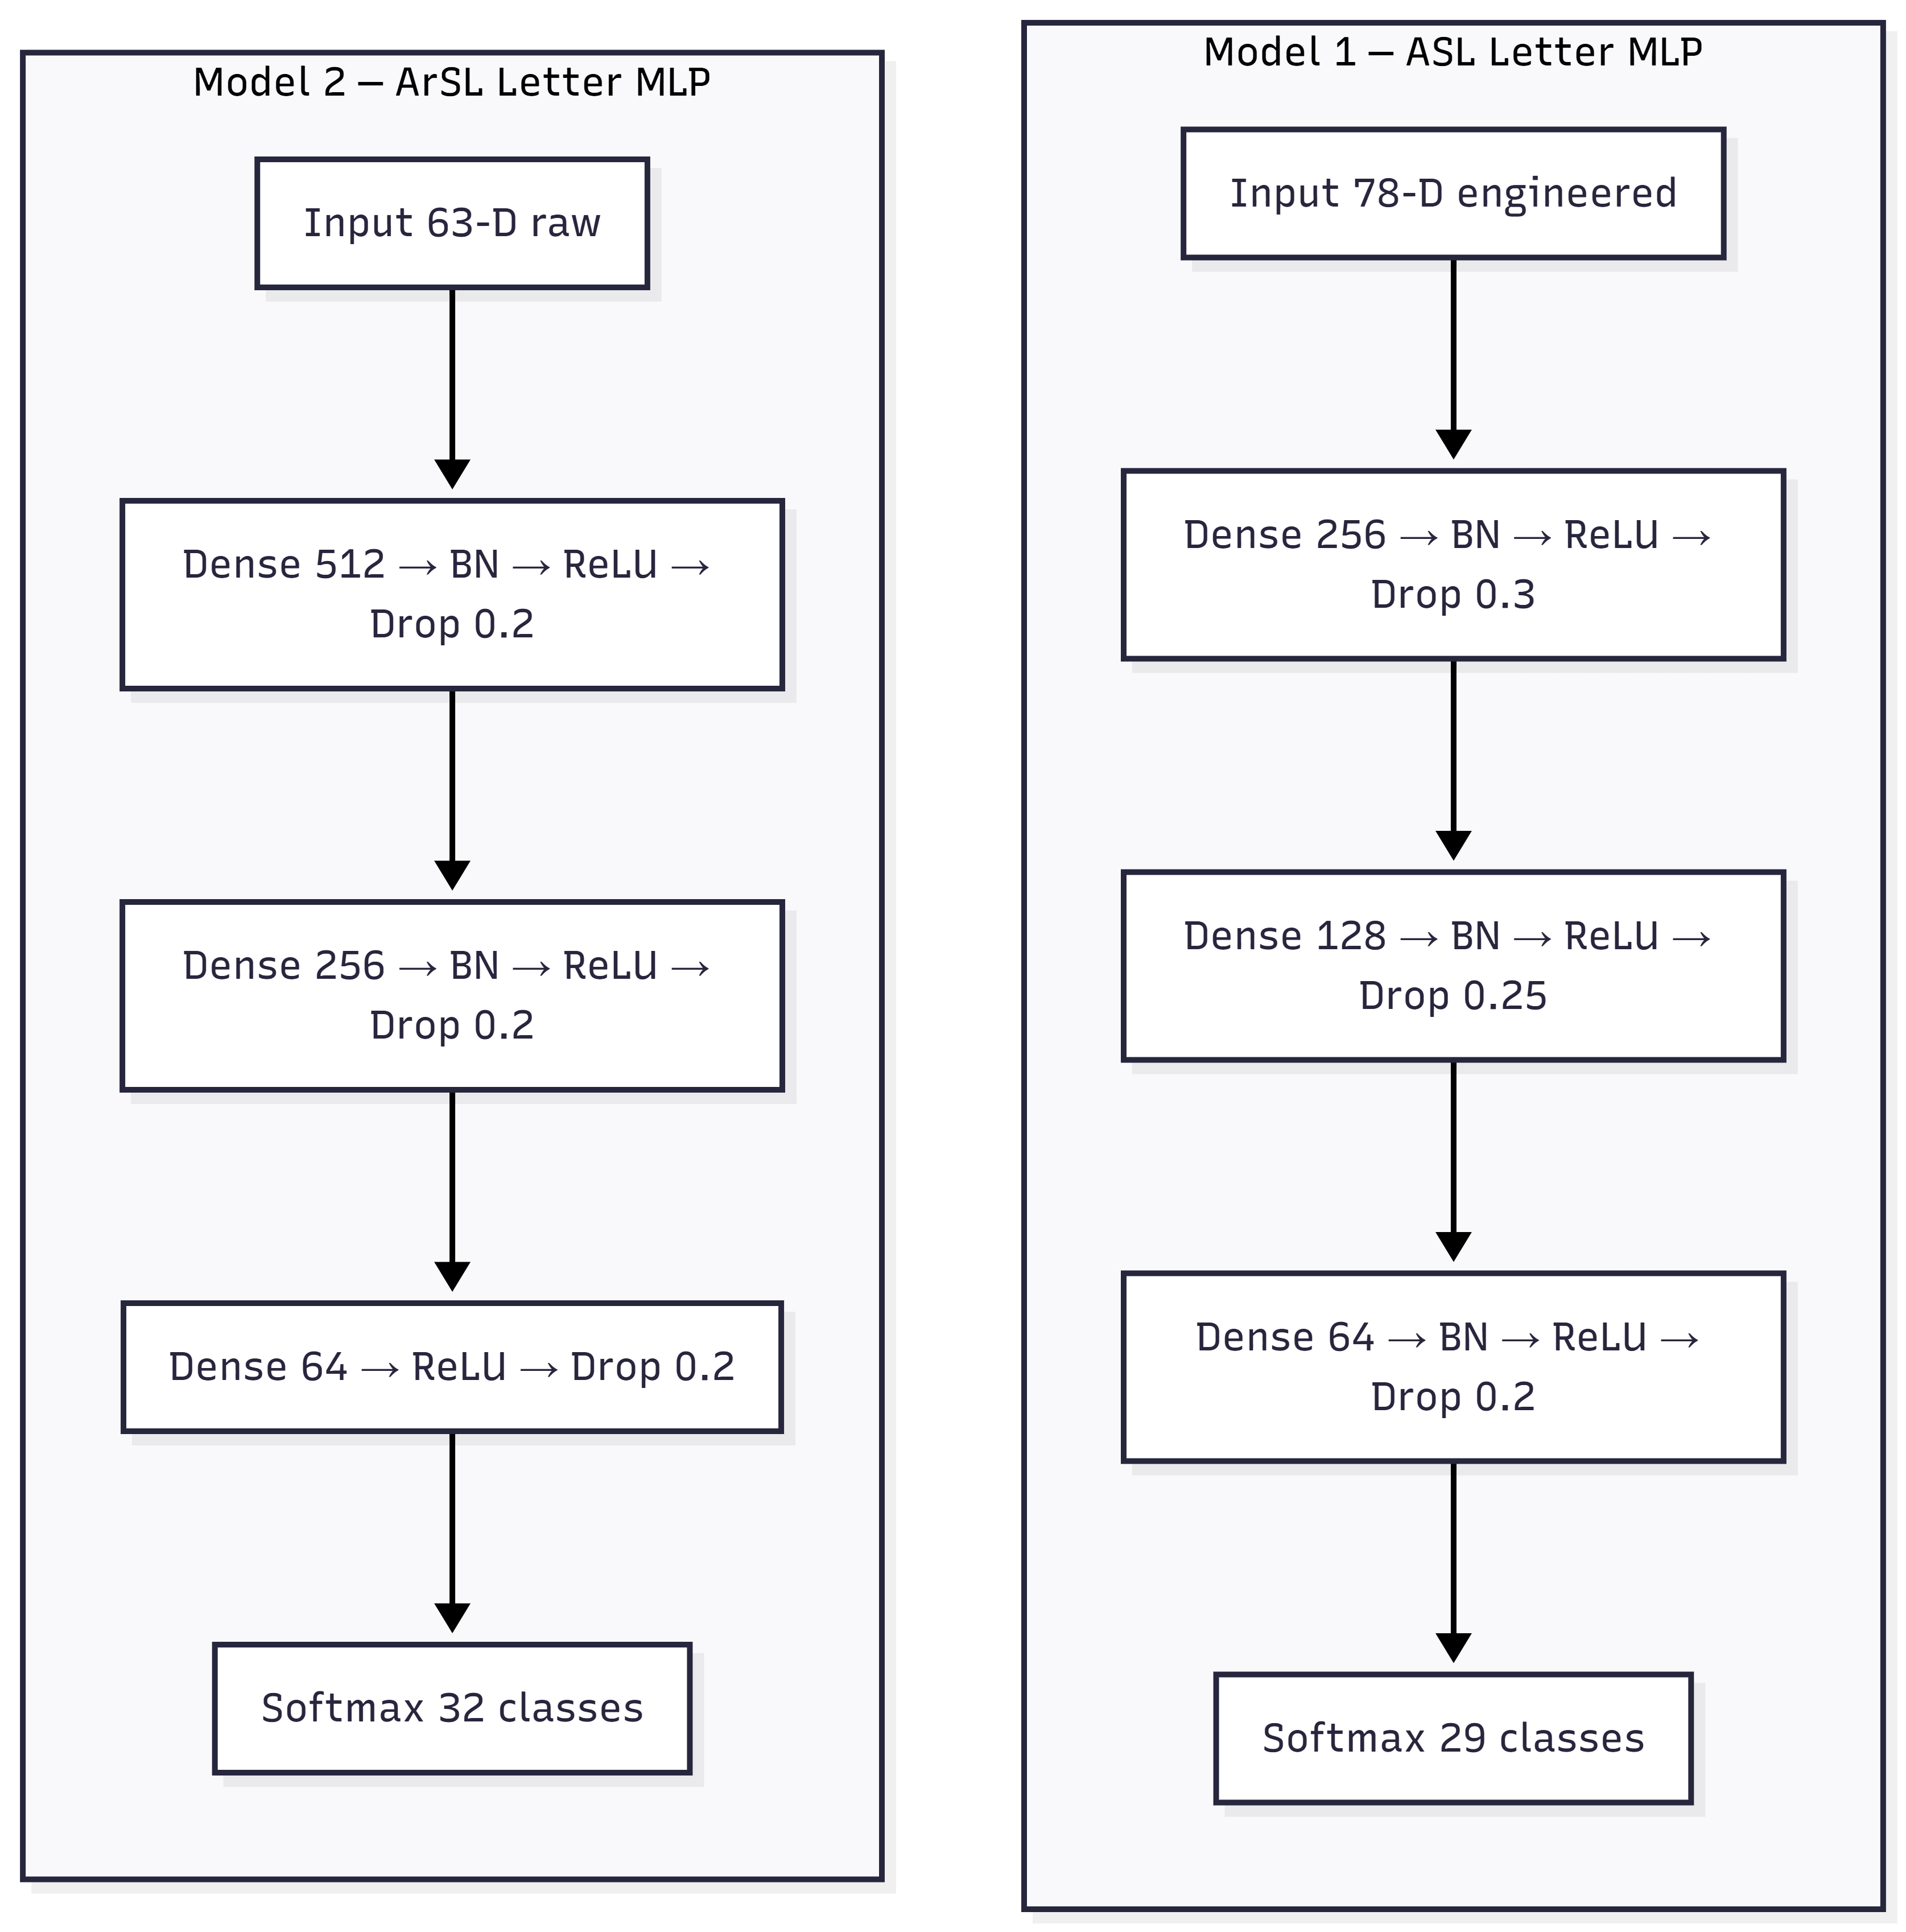
\includegraphics[width=0.88\textwidth]{images/fig_3-9_letter_mlp_heads.png}
\caption{Side-by-side comparison of the two letter MLP heads. Both follow Dense--BN--ReLU--Dropout blocks ending in softmax, but Model~2 uses a wider hidden stack (512/256/64), uniform dropout, and BN on layers~1--2 only.}
\label{fig:ch3-mlp-heads}
\end{figure}
\vspace{0.6cm}

% --- 3.6 STABILISATION ---
\noindent\textbf{3.6\quad LETTER STABILISATION DECODER}\par
\addcontentsline{toc}{section}{\numberline{3.6}LETTER STABILISATION DECODER}
\vspace{0.4cm}

\noindent Per-frame MLP outputs flicker under webcam noise. A finite-state stabilisation policy (as illustrated in Figure~\ref{fig:ch3-stabilisation}) buffers the last \textbf{10} frame labels, commits only when the buffer is full and the dominant label appears in at least \textbf{7 of 10} frames ($\geq$70\,\%), then enforces a \textbf{0.8\,s} hold before the next commit. \texttt{nothing} predictions clear the buffer; duplicate labels during the hold period are suppressed; a new label during hold resets the committed state. These thresholds match the deployed \texttt{letter\_\allowbreak stream\_\allowbreak decoder.py} logic in the FastAPI/React web stack (Chapter~6).\par\vspace{0.3cm}

\noindent A standalone desktop test setup used a stricter policy of 15 frames, 11-of-15 majority, and 1.2\,s hold; those parameters are retained for offline desktop testing but are not part of the web deployment.\par\vspace{0.4cm}

\begin{figure}[H]
\centering
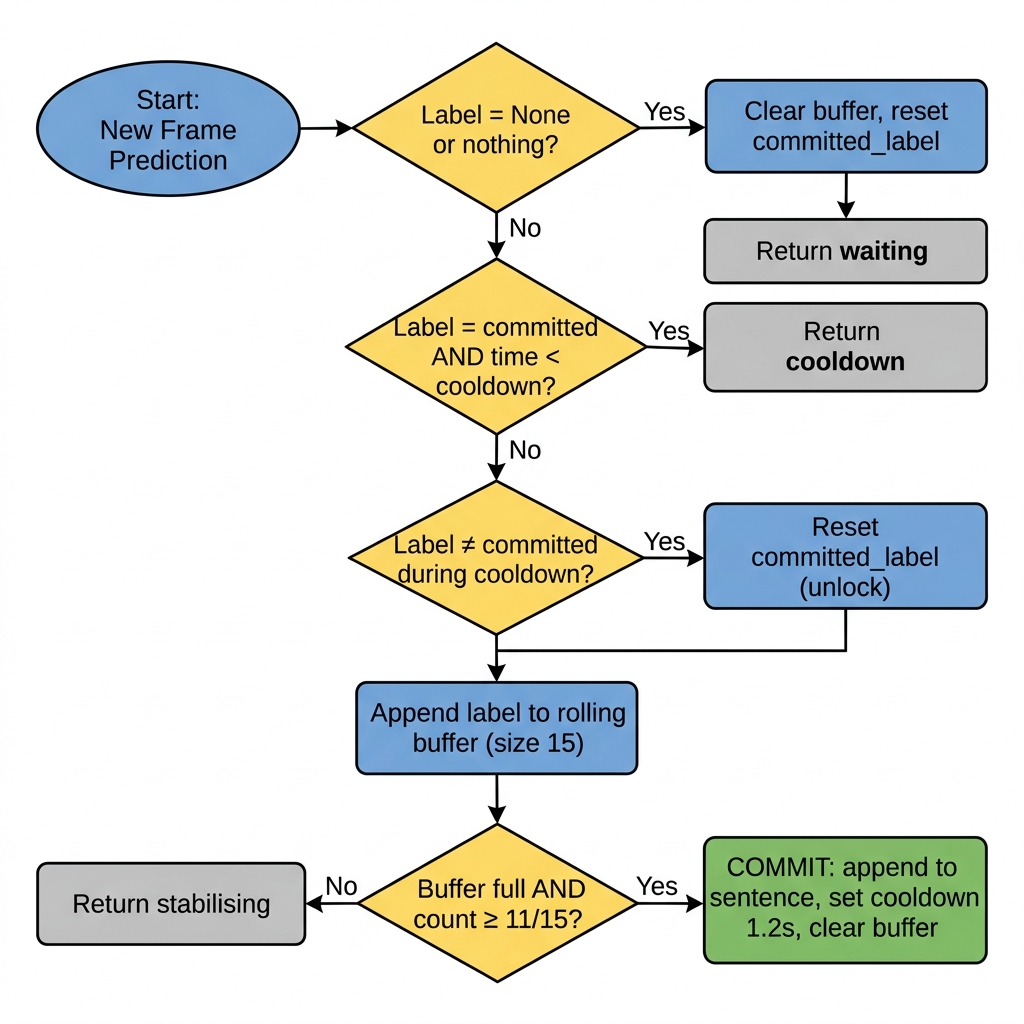
\includegraphics[width=0.75\textwidth]{images/fig_3-4_stabilisation_fsm.png}
\caption{Letter stabilisation finite-state machine. A rolling buffer of 10 frames requires $\geq$7 agreeing labels before \textbf{Commit}; a 0.8\,s hold prevents duplicate characters.}
\label{fig:ch3-stabilisation}
\end{figure}
\vspace{0.6cm}

% --- 3.7 ARABIC RENDERING ---
\noindent\textbf{3.7\quad ARABIC TEXT RENDERING}\par
\addcontentsline{toc}{section}{\numberline{3.7}ARABIC TEXT RENDERING}
\vspace{0.4cm}

\noindent ArSL letter labels are stored as romanised gloss strings (e.g.\ \texttt{bb}). Before display, the UI maps each gloss through \texttt{ARABIC\_MAP} to a Unicode glyph, applies \texttt{arabic\_reshaper}~\cite{arabicreshaper2024} for contextual form selection (isolated/initial/medial/final), reorders with \texttt{python-bidi}~\cite{pythonbidi2024,unicode2021bidirectional}, and renders with PIL/Pillow~\cite{pillow2024} using a TrueType Arabic font on the live HUD frame (as illustrated in Figure~\ref{fig:ch3-arabic-render}). English letter mode skips this pipeline and renders Latin glyphs directly.\par\vspace{0.4cm}

\begin{figure}[H]
\centering
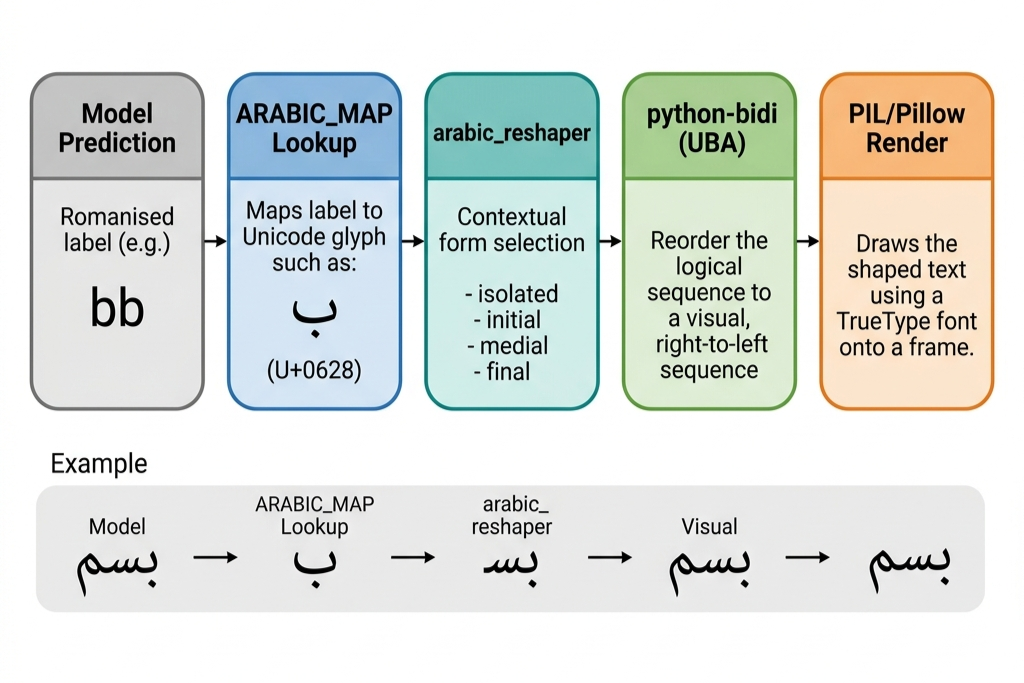
\includegraphics[width=0.9\textwidth]{images/fig_3-6_arabic_rendering.png}
\caption{Arabic UI rendering pipeline. Romanised model labels are mapped to Unicode, reshaped for cursive joining, reordered RTL with python-bidi, and drawn onto the webcam overlay (example: \texttt{bb} $\rightarrow$ ba glyph).}
\label{fig:ch3-arabic-render}
\end{figure}
\vspace{0.6cm}

% --- 3.8 TRADE-OFFS ---

\vspace*{-0.3cm} % Secret trick: Pulls the whole page's starting text slightly up into the top margin

\noindent\textbf{3.8\quad ENGINEERING TRADE-OFFS (LETTERS)}\par
\addcontentsline{toc}{section}{\numberline{3.8}ENGINEERING TRADE-OFFS (LETTERS)}
\vspace{0.2cm} % Cramped from 0.4cm

\begin{table}[H]
\centering
\caption{Engineering trade-offs for letter recognition in Eshara.}
\label{tab:ch3-tradeoffs}
\footnotesize % Shrunk from \small to save vertical space
\begin{tabular}{|p{0.26\textwidth}|p{0.30\textwidth}|p{0.36\textwidth}|}
\hline
\textbf{Decision} & \textbf{Alternative considered} & \textbf{Rationale} \\ \hline
Landmarks not pixels & MobileNetV2 on letter images & Webcam domain gap; unified live path \\ \hline
MLP for letters & BiLSTM per frame & No temporal signal; lower latency \\ \hline
63-D raw (ArSL) / 78-D (ASL) & Single shared feature size & ASL gains from angle features; ArSL stays lightweight \\ \hline
Wider ArSL MLP (512/256/64) & Same 256/128/64 stack as ASL & Higher intra-class variation; similar Arabic letter pairs \\ \hline
Stabilisation decoder & Raw per-frame display & Reduces flicker; improves UX \\ \hline
Web-only deploy & Mobile / TFLite & Graduation scope; WCAG browser access \\ \hline
\end{tabular}
\end{table}
\vspace{0.2cm} % Cramped from 0.6cm
\clearpage
% --- 3.9 EVAL ---
\noindent\textbf{3.9\quad EVALUATION PROTOCOL (LETTERS)}\par
\addcontentsline{toc}{section}{\numberline{3.9}EVALUATION PROTOCOL (LETTERS)}
\vspace{0.2cm} % Cramped from 0.4cm

\noindent Each letter model is evaluated on a \textbf{held-out test split} never used for hyperparameter tuning. Reported metrics (Chapter~6):
\vspace{-0.1cm} % Pulls the bulleted list closer to the sentence above it
\begin{itemize}
\setlength{\itemsep}{0pt} % Removes empty lines between bullet points
\setlength{\parskip}{0pt}
\item \textbf{Top-1 accuracy} --- both letter models.
\item \textbf{Confusion matrices} and per-class precision/recall --- error analysis (motion letters J/Z for ASL; visually similar pairs for ArSL).
\item \textbf{End-to-end latency} (ms) --- letter MLP path including stabilisation (Chapter~5, Section~5.12).
\end{itemize}
\vspace{0.2cm} % Cramped from 0.3cm

\noindent Chapter~4 describes word recognition methodology; Chapter~6 reports measured offline results; Chapter~5 describes the web implementation.\par\vspace{0.2cm}

\enlargethispage{2\baselineskip} % THE MAGIC BULLET: Forces LaTeX to make this specific page 2 lines taller at the bottom margin to catch any spilling text!

\noindent\textbf{Chapter summary.} Letter recognition in Eshara is implemented as two independent single-frame MLP classifiers behind one web API. Both share MediaPipe Hands extraction and the same offline training workflow (as summarised in Figure~\ref{fig:ch3-training-pipeline}), but ASL uses 78-D engineered features with a compact 256/128/64 head ($\sim$49\,k parameters), whereas ArSL uses 63-D raw features with a wider 512/256/64 head ($\sim$183\,k parameters) tuned for visually similar Arabic letter pairs (as compared in Figure~\ref{fig:ch3-mlp-heads} and Table~\ref{tab:ch3-arch-compare}). A stabilisation decoder suppresses per-frame flicker before the UI commits characters; Arabic output passes through a dedicated RTL rendering pipeline. Results for both letter models are reported in Chapter~6.\par

\clearpage
\newpage
% ==========================================
%              CHAPTER FOUR
% ==========================================
\thispagestyle{plain}

\begin{center}
    \vspace*{0.5cm}
    {\large \textit{Chapter Four}} \\[0.4cm]
    {\Large \textbf{4 \quad METHODOLOGY --- WORD RECOGNITION}}
\end{center}
\addcontentsline{toc}{chapter}{\textbf{4 \quad METHODOLOGY --- WORD RECOGNITION}}
\vspace{1in}

\normalsize
\startchapterfloats{4}

\noindent Chapter~3 presented letter-recognition methodology. Chapter~2 Table~\ref{tab:feature-vectors} and Table~\ref{tab:four-models} introduced the hybrid word-input design: ASL words consume buffered RGB clips; ArSL words consume 225-D normalised Holistic sequences. This chapter specifies the full preprocessing equations, model architectures, and model-side inference protocols for \textbf{both} graduation word models --- Model~3 (ASL, Inception I3D) and Model~4 (ArSL, stacked BiLSTM) --- treated symmetrically as standalone Eshara pipelines (web wiring is in Chapter~5). The chapter is divided into two halves: \textbf{Part~A} (Sections~4.1--4.5) and \textbf{Part~B} (Sections~4.6--4.9), followed by a cross-language comparison and evaluation protocol (Sections~4.10--4.12). Quantitative results are reported in Chapter~6~\cite{li2020wlasl,sidig2021karsl,zhang2020mediapipe}.\par\vspace{0.4cm}

\begin{table}[H]
\centering
\caption{Chapter~4 at a glance: side-by-side comparison of both word recognition pipelines.}
\label{tab:ch4-overview}
\small
\begin{tabular}{|P{3.0cm}|P{5.4cm}|P{5.4cm}|}
\hline
\textbf{Property} & \textbf{ASL Words (Model~3)} & \textbf{ArSL Words (Model~4)} \\
\hline
Dataset & WLASL-2000 subset & KArSL-502 (SignID 71--170) \\
Classes & 100 WLASL glosses & 100 Arabic words \\
Input tensor & $(1,3,32,224,224)$ RGB & $(1,48,225)$ Holistic \\
Frames & 32 & 48 \\
Feature source & Raw RGB pixels & MediaPipe Holistic landmarks \\
Architecture & Inception I3D (3-D CNN) & Stacked BiLSTM \\
Parameters & $\sim$12.5\,M & $\sim$255\,K \\
Checkpoint & \texttt{asl\_word\_i3d.pt} & \texttt{arsl\_word\_bilstm.h5} \\
Stabilisation & 6/10 vote, $\geq$50\,\% conf, 1.2\,s & Hand-present gate, rolling deque \\
Test Top-1 & \textbf{65.89\,\%} (WLASL-100 benchmark) & 99.62\,\% \\
\hline
\end{tabular}
\end{table}
\vspace{0.6cm}

% ==========================================================
% PART A: ASL WORD RECOGNITION
% ==========================================================
\begin{center}
\large\textbf{PART A: ASL WORD RECOGNITION (Model~3 --- Inception I3D)}
\end{center}
\addcontentsline{toc}{section}{\textbf{PART A: ASL WORD RECOGNITION (Model 3)}}
\vspace{0.4cm}
\noindent\rule{\textwidth}{0.8pt}
\vspace{0.4cm}

% --- 4.1 WLASL DATASET ---
\noindent\textbf{4.1\quad WLASL DATASET AND SPLIT POLICY}\par
\addcontentsline{toc}{section}{\numberline{4.1}WLASL DATASET AND SPLIT POLICY}
\vspace{0.4cm}

\noindent WLASL-2000 (Word-Level American Sign Language) provides roughly 21\,000 video clips across 2\,000 glosses sourced from public sign-language instructional portals~\cite{li2020wlasl,li2020wlaslgithub}. Table~\ref{tab:ch4-wlasl-stats} summarises the corpus properties relevant to Model~3.\par\vspace{0.4cm}

\begin{table}[H]
\centering
\caption{WLASL dataset statistics for the Model~3 (ASL word) graduation deployment.}
\label{tab:ch4-wlasl-stats}
\small
\renewcommand{\arraystretch}{1.4} % Adds vertical padding so the text doesn't hit the borders
\begin{tabular}{|P{4.5cm}|P{9.0cm}|}
\hline
\textbf{Property} & \textbf{Value} \\ \hline
Full corpus size & $\sim$21\,000 clips, 2\,000 glosses \\ \hline
Graduation subset & 100 classes (WLASL-100) \\ \hline
Avg.\ clips / class & 10--200 (highly variable; broken download URLs reduce effective coverage) \\ \hline
Frame rate & Variable; clips resampled to 32 frames at inference \\ \hline
Frame resolution & Resized to 256 then centre-cropped to 224$\times$224 per frame \\ \hline
Input format & Raw RGB, normalised to $[-1,1]$ \\ \hline
Pre-trained checkpoint & \texttt{asl\_\allowbreak word\_\allowbreak i3d.pt} (Kinetics-400 backbone, 100-class WLASL head) \\ \hline
Test split & WLASL held-out test partition (not used in fine-tuning) \\ \hline
\end{tabular}
\end{table}
\vspace{0.4cm}

\noindent WLASL clip counts vary widely across glosses. Eshara's ASL word model therefore uses a \textbf{pretrained Inception I3D} checkpoint: a Kinetics-400 backbone with a 100-way WLASL classification head, deployed within graduation GPU limits rather than trained from scratch on the full 2\,000-gloss corpus~\cite{li2020wlasl}.\par\vspace{0.6cm}

% --- 4.2 ASL FEATURE EXTRACTION ---
\clearpage
\noindent\textbf{4.2\quad ASL FEATURE EXTRACTION --- RGB CLIP PIPELINE}\par
\addcontentsline{toc}{section}{\numberline{4.2}ASL FEATURE EXTRACTION --- RGB CLIP PIPELINE}
\vspace{0.4cm}

\noindent Model~3 does \emph{not} use MediaPipe landmarks. Raw webcam frames pass through a four-step preprocessing chain (Table~\ref{tab:ch4-asl-preproc}) and are buffered into a 32-frame clip tensor before the I3D forward pass.\par\vspace{0.4cm}

\begin{table}[H]
\centering
\caption{ASL RGB clip preprocessing steps (per frame, Model~3).}
\label{tab:ch4-asl-preproc}
\small
\renewcommand{\arraystretch}{1.4} % Adds vertical padding so the text doesn't hit the borders
\begin{tabular}{|c|P{3.5cm}|P{3.5cm}|P{3.5cm}|P{3.5cm}|}
\hline
\textbf{Step} & \textbf{Operation} & \textbf{Input shape} & \textbf{Output shape} & \textbf{Library} \\ \hline
1 & BGR $\rightarrow$ RGB colour convert & $(H, W, 3)$ uint8 & $(H, W, 3)$ uint8 & \texttt{cv2} \\ \hline
2 & Aspect-preserving resize (short side $= 256$) & $(H, W, 3)$ & $(H', W', 3)$ & \texttt{cv2.\allowbreak INTER\_\allowbreak LINEAR} \\ \hline
3 & Centre crop $224\!\times\!224$ & $(H', W', 3)$ & $(224, 224, 3)$ & Slice \\ \hline
4 & Normalise: $\tilde{I} = (I / 255)\times 2 - 1$ & $[0, 255]$ int & $[-1, 1]$ float32 & NumPy \\ \hline
5 & Transpose to $(C, H, W)$ & $(224, 224, 3)$ & $(3, 224, 224)$ & \texttt{.transpose\allowbreak(2,0,1)} \\ \hline
6 & Stack 32 frames & 32$\times(3, 224, 224)$ & $(3, 32, 224, 224)$ & \texttt{np.stack} \\ \hline
7 & Batch (unsqueeze) & $(3, 32, 224, 224)$ & $(1, 3, 32, 224, 224)$ & \texttt{torch.\allowbreak unsqueeze} \\ \hline
\end{tabular}
\end{table}
\vspace{0.4cm}

\noindent\textbf{Step 2 --- Aspect-preserving resize.} The scale factor $\alpha$ preserves the aspect ratio while guaranteeing that the shorter dimension reaches exactly 256:
\begin{equation}
s = \min(H, W), \qquad \alpha = \frac{256}{s}, \qquad H' = \lfloor H\alpha + 0.5 \rfloor,\quad W' = \lfloor W\alpha + 0.5 \rfloor.
\label{eq:ch4-resize}
\end{equation}

\noindent\textbf{Step 3 --- Centre crop.} A $224\times 224$ patch is extracted around the spatial centre $(c_y, c_x) = (H'/2, W'/2)$:
\begin{equation}
I_{\text{crop}} = I'[\,c_y - 112 \;:\; c_y + 112,\;\; c_x - 112 \;:\; c_x + 112\,] \in \mathbb{Z}^{224 \times 224 \times 3}.
\label{eq:ch4-crop}
\end{equation}

\noindent\textbf{Step 4 --- Normalisation.} Pixel values are linearly mapped from $[0,\,255]$ to $[-1,\,1]$, matching the normalisation convention used at training time for Model~3:
\begin{equation}
\tilde{I} = \frac{I_{\text{crop}}}{255.0} \times 2.0 - 1.0 \in [-1,\,1]^{224 \times 224 \times 3}.
\label{eq:ch4-pixelnorm}
\end{equation}

\noindent\textbf{Clip assembly (Steps 6--7).} Processed frames accumulate in a rolling \texttt{deque(maxlen=32)}. When full, frames are stacked along the temporal axis and wrapped in a batch dimension:
\begin{equation}
\mathbf{V} = \bigl[\tilde{I}_1,\ldots,\tilde{I}_{32}\bigr] \in \mathbb{R}^{3 \times 32 \times 224 \times 224}, \qquad \hat{\mathbf{V}} = \mathbf{V}.\mathrm{unsqueeze}(0) \in \mathbb{R}^{1 \times 3 \times 32 \times 224 \times 224}.
\label{eq:ch4-clip}
\end{equation}
The PyTorch I3D implementation requires the tensor in $(N, C, T, H, W)$ order; this is opposite to TensorFlow's $(N, T, H, W, C)$ convention used by the ArSL model.\par\vspace{0.4cm}

\begin{figure}[H]
\centering
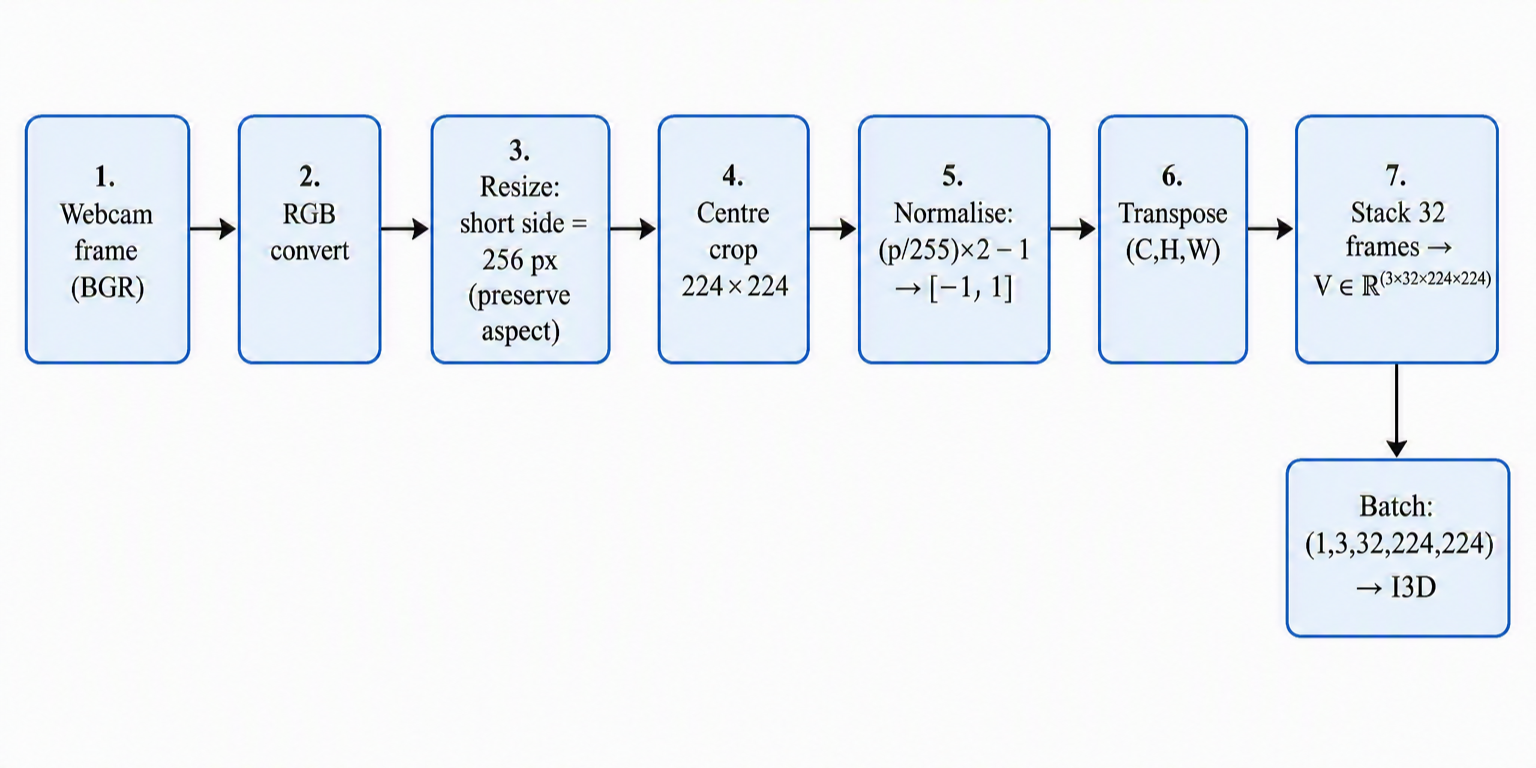
\includegraphics[width=0.95\textwidth]{images/fig_4-1_asl_rgb_preprocess.png}
\caption{ASL word RGB clip preprocessing (Model~3). Each frame passes through colour conversion, aspect-preserving resize (short side 256\,px), centre crop $224\!\times\!224$, $[-1,1]$ normalisation, and $(C,H,W)$ transpose before accumulation in a 32-frame deque (Table~\ref{tab:ch4-asl-preproc}, Equations~\eqref{eq:ch4-resize}--\eqref{eq:ch4-clip}).}
\label{fig:ch4-asl-preprocess}
\end{figure}
\vspace{0.6cm}
\clearpage
% --- 4.3 MODEL 3: INCEPTION I3D ---
\noindent\textbf{4.3\quad MODEL 3 --- ASL WORD INCEPTION I3D}\par
\addcontentsline{toc}{section}{\numberline{4.3}MODEL 3 --- ASL WORD INCEPTION I3D}
\vspace{0.4cm}

\noindent\textbf{Problem.} ASL word meaning depends on hand shape, arm trajectory, and whole-body motion across roughly one second of video. A per-frame landmark vector cannot capture the spatio-temporal dynamics that distinguish glosses with similar handshapes but different movement paths~\cite{li2020wlasl}.\par\vspace{0.4cm}

\noindent\textbf{4.3.1\quad Architectural Family --- Inflated 3-D ConvNet:}\par
\addcontentsline{toc}{subsection}{\numberline{4.3.1}Architectural Family --- Inflated 3-D ConvNet:}
\vspace{0.3cm}

\noindent Inception I3D (Carreira \& Zisserman, 2017) extends the Inception-v1 image backbone by replacing every 2-D convolution filter $k_h \times k_w$ with a volumetric filter $k_t \times k_h \times k_w$ that operates jointly over time and space~\cite{li2020wlasl}. The ``inflation'' initialisation bootstraps 3-D weights from pretrained 2-D ImageNet weights by replicating each filter along the temporal axis and dividing by $k_t$:
\begin{equation}
W^{3\text{D}}_{:,:,\,t,:,:} = \frac{W^{2\text{D}}}{k_t}, \qquad t = 1,\ldots,k_t,
\label{eq:ch4-inflate}
\end{equation}
so that the initial response to a static frame matches the 2-D pretrained response. This allows the model to start from spatially rich ImageNet features and adapt to motion during fine-tuning on video data.\par\vspace{0.3cm}

\noindent\textbf{4.3.2\quad Building Block --- Unit3D:}\par
\addcontentsline{toc}{subsection}{\numberline{4.3.2}Building Block --- Unit3D:}
\vspace{0.3cm}

\noindent Every convolutional stage is implemented as a \textbf{Unit3D} block: a 3-D convolution with dynamically computed SAME padding, followed by Batch Normalisation and ReLU. For a feature volume $\mathbf{A} \in \mathbb{R}^{N \times C_{\text{in}} \times T' \times H' \times W'}$ and filter bank $\mathbf{F} \in \mathbb{R}^{C_{\text{out}} \times C_{\text{in}} \times k_t \times k_h \times k_w}$:
\begin{equation}
(\mathbf{A} \!\ast\! \mathbf{F})_{n,c,t,h,w} = \sum_{c'} \sum_{\delta_t} \sum_{\delta_h} \sum_{\delta_w} \mathbf{A}_{n,c',\,t+\delta_t,\,h+\delta_h,\,w+\delta_w} \cdot \mathbf{F}_{c,c',\,\delta_t,\delta_h,\delta_w}.
\label{eq:ch4-3dconv}
\end{equation}
Batch Normalisation~\cite{ioffe2015batchnorm} stabilises activations across the training batch:
\begin{equation}
\mathbf{Z} = \mathrm{ReLU}\!\left(\gamma\,\frac{\mathbf{A}\!\ast\!\mathbf{F} - \mu_B}{\sqrt{\sigma_B^2 + \varepsilon}} + \beta\right), \qquad \varepsilon = 10^{-3},
\label{eq:ch4-bn}
\end{equation}
where $\mu_B, \sigma_B^2$ are the per-channel batch mean and variance, and $\gamma, \beta$ are learned scale and shift parameters ($\varepsilon = 10^{-3}$).\par\vspace{0.3cm}
\clearpage
\noindent\textbf{4.3.3\quad InceptionModule --- 4-Branch Parallel Block:}\par
\addcontentsline{toc}{subsection}{\numberline{4.3.3}InceptionModule --- 4-Branch Parallel Block:}
\vspace{0.3cm}

\noindent Each Inception stage runs four branches in parallel and channel-concatenates their outputs. For input $\mathbf{A}$ with $C_{\text{in}}$ channels and branch output sizes $[n_0, n_{1a}, n_{1b}, n_{2a}, n_{2b}, n_{3b}]$:
\begin{align}
\text{Branch~0 (direct):}\quad & \mathbf{B}_0 = \mathrm{Unit3D}(\mathbf{A};\;1\!\times\!1\!\times\!1,\;n_0), \label{eq:ch4-b0} \\
\text{Branch~1 (bottleneck+3$\times$3):}\quad & \mathbf{B}_1 = \mathrm{Unit3D}\!\bigl(\mathrm{Unit3D}(\mathbf{A};\;1\!\times\!1\!\times\!1,\;n_{1a});\;3\!\times\!3\!\times\!3,\;n_{1b}\bigr), \label{eq:ch4-b1} \\
\text{Branch~2 (bottleneck+3$\times$3):}\quad & \mathbf{B}_2 = \mathrm{Unit3D}\!\bigl(\mathrm{Unit3D}(\mathbf{A};\;1\!\times\!1\!\times\!1,\;n_{2a});\;3\!\times\!3\!\times\!3,\;n_{2b}\bigr), \label{eq:ch4-b2} \\
\text{Branch~3 (pool+project):}\quad & \mathbf{B}_3 = \mathrm{Unit3D}\!\bigl(\mathrm{MaxPool}_{3\times3\times3}(\mathbf{A});\;1\!\times\!1\!\times\!1,\;n_{3b}\bigr). \label{eq:ch4-b3}
\end{align}
\begin{equation}
\mathrm{InceptionModule}(\mathbf{A}) = \mathrm{Concat}(\mathbf{B}_0, \mathbf{B}_1, \mathbf{B}_2, \mathbf{B}_3) \in \mathbb{R}^{N \times (n_0 + n_{1b} + n_{2b} + n_{3b}) \times T' \times H' \times W'}.
\label{eq:ch4-incept}
\end{equation}
The $1\!\times\!1\!\times\!1$ bottlenecks in Branches~1--3 reduce channel depth before the more expensive $3\!\times\!3\!\times\!3$ convolutions, capturing multi-scale context efficiently. Branch~3 uses max-pooling followed by a $1\!\times\!1\!\times\!1$ projection, providing a pooling path without additional 3-D convolution cost.\par\vspace{0.4cm}

\begin{figure}[H]
\centering
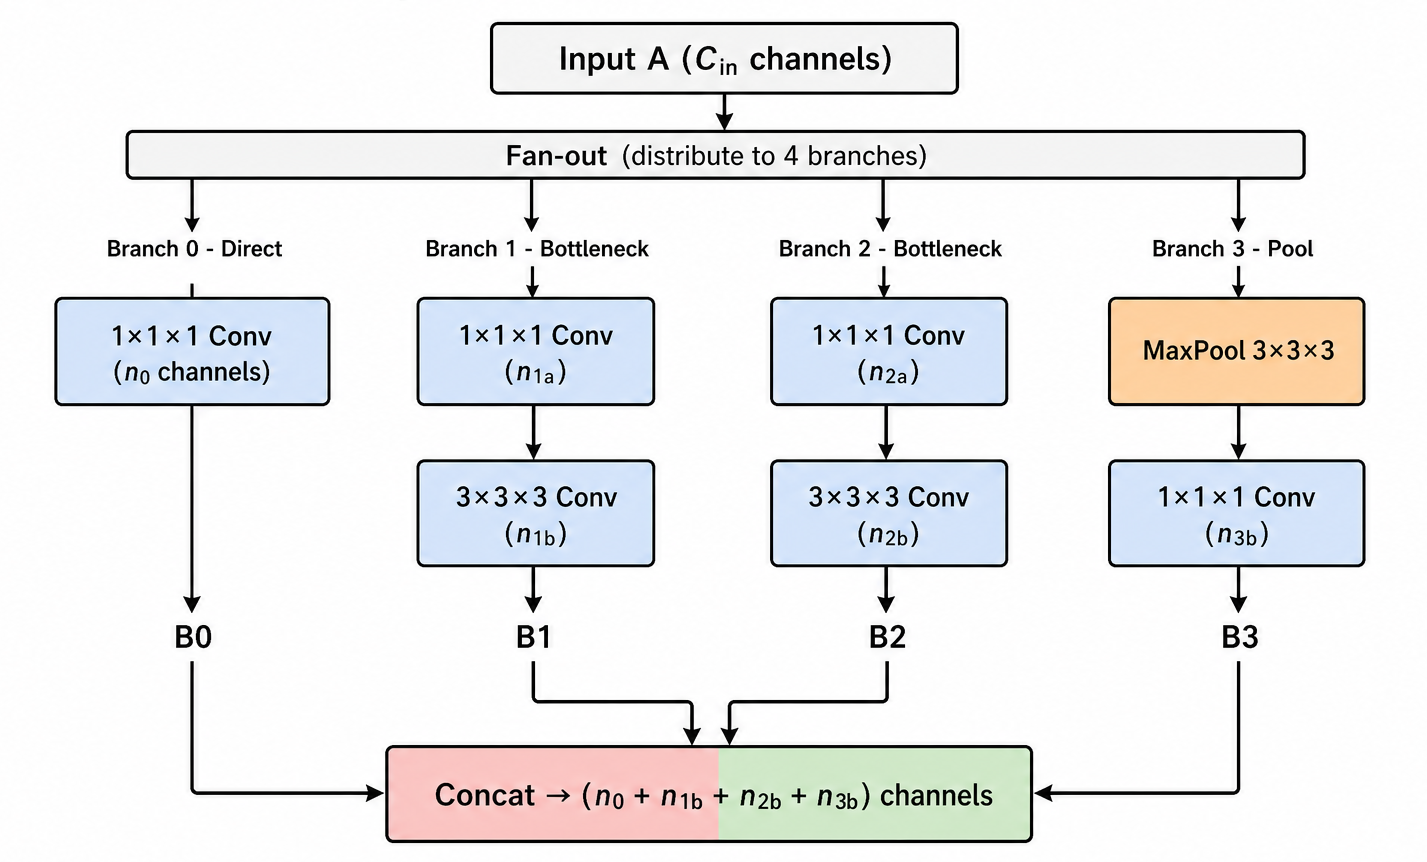
\includegraphics[width=0.99\textwidth]{images/fig_4-9_inception_module.png}
\caption{InceptionModule 4-branch parallel structure (Equations~\eqref{eq:ch4-b0}--\eqref{eq:ch4-incept}). All branches process the same input $\mathbf{A}$ simultaneously; outputs are channel-concatenated. Example for \texttt{Mixed\_3b}: $[64, 96, 128, 16, 32, 32] \rightarrow 64+128+32+32 = 256$ output channels.}
\label{fig:ch4-inception-branches}
\end{figure}
\vspace{0.4cm}

\noindent\textbf{4.3.4\quad Full Layer Stack:}\par
\addcontentsline{toc}{subsection}{\numberline{4.3.4}Full Layer Stack:}
\vspace{0.3cm}

\noindent Table~\ref{tab:ch4-i3d-stack} lists every stage in order for Model~3. The input enters as $\hat{\mathbf{V}} \in \mathbb{R}^{1 \times 3 \times 32 \times 224 \times 224}$.

\begin{table}[H]
\centering
\caption{Inception I3D layer stack (Model~3, ASL words). Branch configs for Inception stages: $[n_0, n_{1a}, n_{1b}, n_{2a}, n_{2b}, n_{3b}]$ per Equation~\eqref{eq:ch4-incept}. Input: $(1, 3, 32, 224, 224)$.}
\label{tab:ch4-i3d-stack}
\footnotesize
\renewcommand{\arraystretch}{1.6} % Adds vertical padding so the text doesn't hit the borders
\resizebox{\textwidth}{!}{%
\begin{tabular}{|c|l|l|c|l|}
\hline
\textbf{\#} & \textbf{Stage name} & \textbf{Layer type} & \textbf{Out ch.} & \textbf{Config / notes} \\ \hline
1 & Conv3d\_1a\_7x7 & Unit3D & 64 & kernel $7\!\times\!7\!\times\!7$, stride $(2,2,2)$, padding $3$ \\ \hline
2 & MaxPool3d\_2a\_3x3 & MaxPool3d (SAME) & 64 & kernel $(1,3,3)$, stride $(1,2,2)$ \\ \hline
3 & Conv3d\_2b\_1x1 & Unit3D & 64 & kernel $1\!\times\!1\!\times\!1$ \\ \hline
4 & Conv3d\_2c\_3x3 & Unit3D & 192 & kernel $3\!\times\!3\!\times\!3$ \\ \hline
5 & MaxPool3d\_3a\_3x3 & MaxPool3d (SAME) & 192 & kernel $(1,3,3)$, stride $(1,2,2)$ \\ \hline
6 & Mixed\_3b & InceptionModule & 256 & $[64,\;96,\;128,\;16,\;32,\;32]$ \\ \hline
7 & Mixed\_3c & InceptionModule & 480 & $[128,\;128,\;192,\;32,\;96,\;64]$ \\ \hline
8 & MaxPool3d\_4a\_3x3 & MaxPool3d (SAME) & 480 & kernel $(3,3,3)$, stride $(2,2,2)$ \\ \hline
9 & Mixed\_4b & InceptionModule & 512 & $[192,\;96,\;208,\;16,\;48,\;64]$ \\ \hline
10 & Mixed\_4c & InceptionModule & 512 & $[160,\;112,\;224,\;24,\;64,\;64]$ \\ \hline
11 & Mixed\_4d & InceptionModule & 512 & $[128,\;128,\;256,\;24,\;64,\;64]$ \\ \hline
12 & Mixed\_4e & InceptionModule & 528 & $[112,\;144,\;288,\;32,\;64,\;64]$ \\ \hline
13 & Mixed\_4f & InceptionModule & 832 & $[256,\;160,\;320,\;32,\;128,\;128]$ \\ \hline
14 & MaxPool3d\_5a\_2x2 & MaxPool3d & 832 & kernel $(2,2,2)$, stride $(2,2,2)$ \\ \hline
15 & Mixed\_5b & InceptionModule & 832 & $[256,\;160,\;320,\;32,\;128,\;128]$ \\ \hline
16 & Mixed\_5c & InceptionModule & 1024 & $[384,\;192,\;384,\;48,\;128,\;128]$ \\ \hline
17 & AvgPool3d & nn.AvgPool3d & 1024 & kernel $(2,7,7)$, stride $(1,1,1)$ \\ \hline
18 & Dropout & nn.Dropout & 1024 & $p = 0.5$ \\ \hline
19 & Logits (Unit3D) & 3-D conv & \textbf{100} & $1\!\times\!1\!\times\!1$, no BN, no activation, bias=True \\ \hline
\end{tabular}%
}
\end{table}
\vspace{0.4cm}

\begin{figure}[H]
\centering
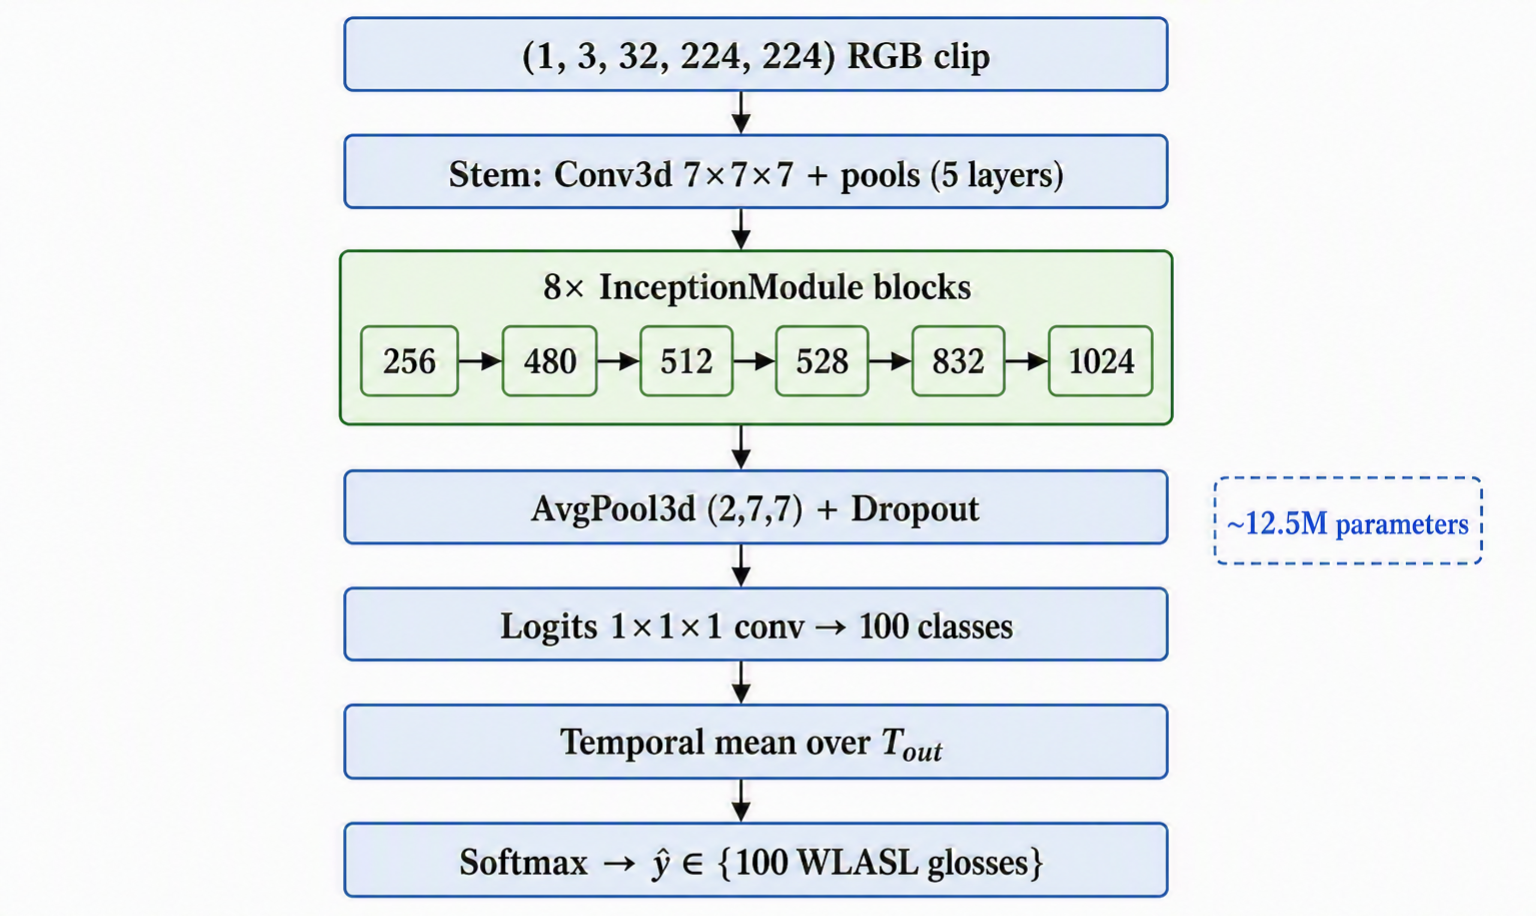
\includegraphics[width=0.99\textwidth]{images/fig_4-2_i3d_forward_pass.png}
\caption{Inception I3D forward pass (Model~3). The $(1,3,32,224,224)$ clip passes through the stem, eight Inception modules (Table~\ref{tab:ch4-i3d-stack}), AvgPool, dropout, and a 100-way logit head; logits are temporally averaged before softmax (Equations~\eqref{eq:ch4-temporal-mean}--\eqref{eq:ch4-i3d-softmax}).}
\label{fig:ch4-i3d-flow}
\end{figure}
\vspace{0.4cm}

\noindent\textbf{4.3.5\quad Temporal Logit Aggregation and Softmax:}\par
\addcontentsline{toc}{subsection}{\numberline{4.3.5}Temporal Logit Aggregation and Softmax:}
\vspace{0.3cm}

\noindent After the forward pass, the logit layer produces a tensor $\mathbf{L} \in \mathbb{R}^{1 \times 100 \times T_{\text{out}}}$ (residual temporal dimension after AvgPool). The spatial dimensions have already been squeezed. Logits are averaged across the residual time axis before softmax:
\begin{equation}
\bar{\mathbf{z}} = \frac{1}{T_{\text{out}}} \sum_{\tau=1}^{T_{\text{out}}} \mathbf{L}_{0,:,\,\tau} \in \mathbb{R}^{100},
\label{eq:ch4-temporal-mean}
\end{equation}
\begin{equation}
P(y{=}k \mid \hat{\mathbf{V}}) = \frac{\exp(\bar{z}_k)}{\displaystyle\sum_{j=1}^{100} \exp(\bar{z}_j)}, \qquad \hat{y} = \arg\max_k P(y{=}k \mid \hat{\mathbf{V}}).
\label{eq:ch4-i3d-softmax}
\end{equation}
Averaging logits before softmax (late temporal fusion on logit space) is numerically more calibrated than averaging softmax probabilities independently~\cite{li2020wlasl}.\par\vspace{0.3cm}
\clearpage
\noindent\textbf{4.3.6\quad Checkpoint and Parameter Count:}\par
\addcontentsline{toc}{subsection}{\numberline{4.3.6}Checkpoint and Parameter Count:}
\vspace{0.3cm}

\noindent Model~3 is initialised as Inception I3D with a 400-class Kinetics head, the logit layer is replaced for $C{=}100$ WLASL glosses, and pretrained weights are loaded from \texttt{asl\_word\_i3d.pt}. At inference, batch normalisation running statistics are frozen and dropout is disabled.\par\vspace{0.2cm}

\noindent\textbf{Parameter count.} The Kinetics-400 backbone contributes $\sim$12.7\,M parameters; replacing the 400-class head ($1024 \times 400 + 400 = 409\,600$ params) with a 100-class head ($1024 \times 100 + 100 = 102\,500$ params) reduces the total by $\sim$307\,K, giving approximately \textbf{12.5 million} parameters for Model~3.\par\vspace{0.6cm}

% --- 4.4 ASL STABILISATION ---
\noindent\textbf{4.4\quad ASL WORD STABILISATION DECODER}\par
\addcontentsline{toc}{section}{\numberline{4.4}ASL WORD STABILISATION DECODER}
\vspace{0.4cm}

\noindent Per-clip I3D predictions can be noisy if a signing motion is captured mid-gesture or the frame buffer transitions between two words. Eshara's \textbf{ASL word stabilisation decoder} suppresses premature or repeated commits using three jointly-evaluated conditions (Table~\ref{tab:ch4-stab-params}):\par\vspace{0.3cm}

\begin{table}[H]
\centering
\caption{ASL word stabilisation parameters (Model~3).}
\label{tab:ch4-stab-params}
\small
\renewcommand{\arraystretch}{1.6}% Adds vertical padding so the text doesn't hit the borders
\begin{tabular}{|P{4.0cm}|c|P{7.2cm}|}
\hline
\textbf{Parameter} & \textbf{Value} & \textbf{Role} \\ \hline
\texttt{FRAME\_BUFFER\_SIZE} & 32 & Frames buffered per inference call \\ \hline
\texttt{STAB\_WINDOW} & 10 & Recent predictions evaluated for voting \\ \hline
\texttt{STAB\_THRESH} & 6 & Minimum matching predictions to consider committing \\ \hline
\texttt{MIN\_CONFIDENCE} & 0.50 & Minimum softmax probability to accept a prediction \\ \hline
\texttt{HOLD\_COOLDOWN} & 1.2\,s & Lock-out period after any commit \\ \hline
Repeat cooldown & 2.4\,s & Lock-out for committing the same word twice \\ \hline
\end{tabular}
\end{table}
\vspace{0.4cm}

\noindent A word is committed when \textbf{all} three conditions simultaneously hold:
\begin{enumerate}
\item \textbf{Majority agreement:} the mode of the last 10 predictions appears $\geq 6$ times.
\item \textbf{Confidence gate:} $\max_k P(y{=}k \mid \hat{\mathbf{V}}) \geq 0.50$.
\item \textbf{Cooldown gate:} $t_{\text{now}} - t_{\text{last\_commit}} > 1.2$\,s (or $> 2.4$\,s for the same word).
\end{enumerate}
On commit, both the frame deque and prediction window are cleared. The endpoint returns \texttt{\{"status":"committed",\ldots\}} or \texttt{\{"status":"buffering",\ldots\}} between commits (Figure~\ref{fig:ch4-asl-stab}).\par\vspace{0.4cm}
\begin{figure}[H]
\centering
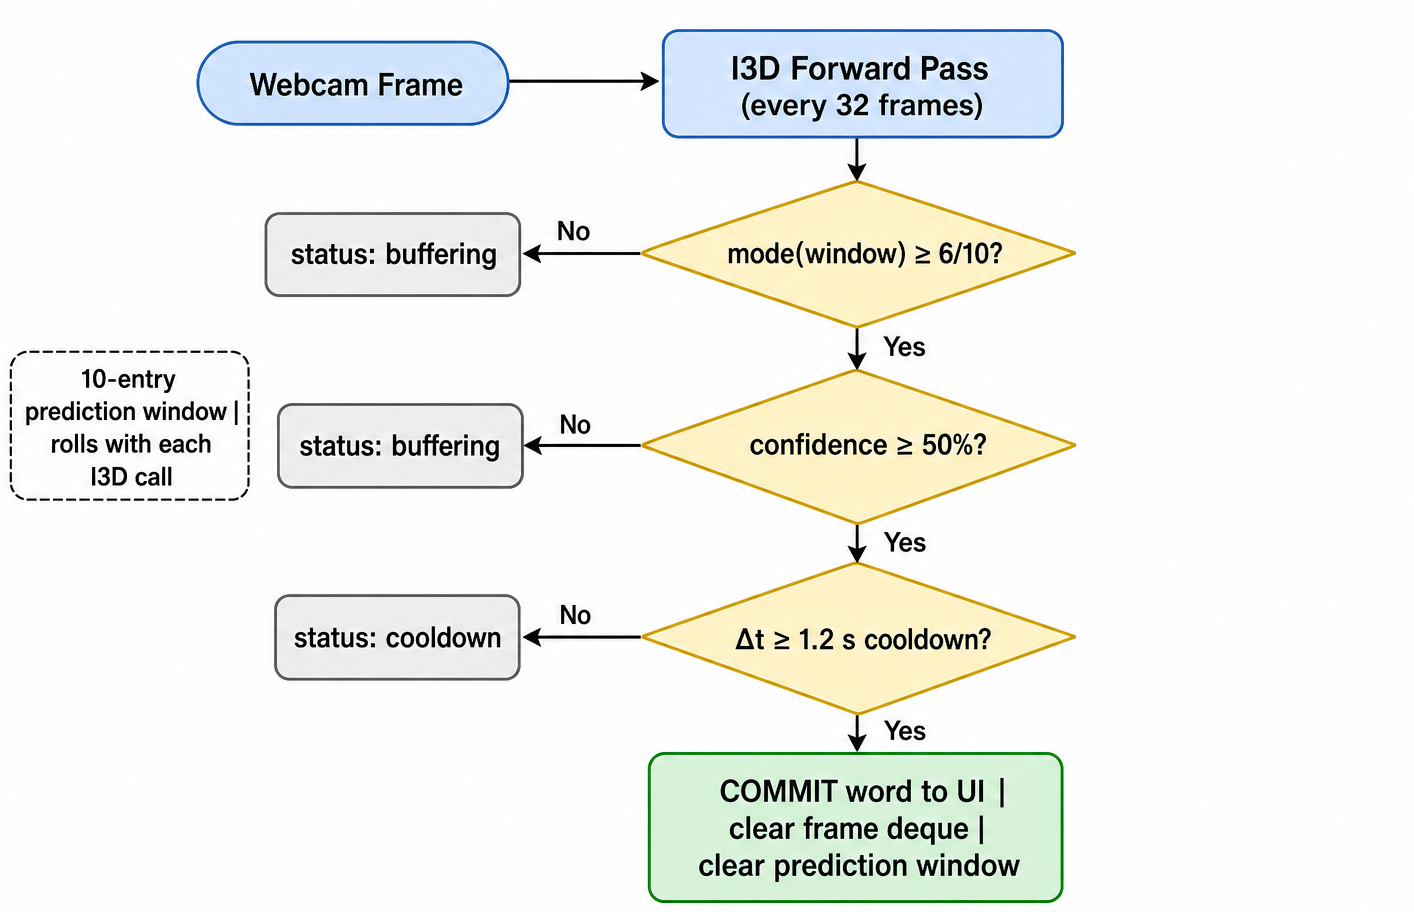
\includegraphics[width=0.82\textwidth]{images/fig_4-8_asl_word_stabiliser.png}
\caption{ASL word stabilisation decoder (Model~3). Three gates --- majority vote (6/10), confidence ($\geq$50\,\%), and cooldown ($\geq$1.2\,s) --- must pass before a gloss is committed (Table~\ref{tab:ch4-stab-params}).}
\label{fig:ch4-asl-stab}
\end{figure}
\vspace{0.2cm} % Cramped from 0.4cm

% --- 4.5 ASL INFERENCE PATH ---
\noindent\textbf{4.5\quad ASL INFERENCE PATH (End-to-End)}\par
\addcontentsline{toc}{section}{\numberline{4.5}ASL INFERENCE PATH (END-TO-END)}
\vspace{0.2cm} % Cramped from 0.4cm

\noindent The model-side path from a single RGB frame to a committed gloss probability vector is:
\vspace{-0.1cm} % Pulled list closer to intro text

\begin{enumerate}
\setlength{\itemsep}{0pt} % Cramped list spacing
\setlength{\parskip}{0pt}
\item Each incoming frame is preprocessed via Steps 1--5 of Table~\ref{tab:ch4-asl-preproc} and appended to a 32-frame rolling buffer.
\item When the buffer is full, frames are stacked to $\mathbf{V} \in \mathbb{R}^{3 \times 32 \times 224 \times 224}$ and batched as $(1,3,32,224,224)$.
\item The I3D forward pass (Equations~\eqref{eq:ch4-3dconv}--\eqref{eq:ch4-i3d-softmax}) returns logits; temporal averaging and softmax produce a 100-D probability vector.
\item The stabilisation decoder (Section~4.4) gates whether a gloss is committed to the UI.
\end{enumerate}
\vspace{0.2cm} % Cramped from 0.3cm

\enlargethispage{\baselineskip} % Extends page bottom margin by 1 line to catch spilling text

\noindent HTTP routing, session management, and the React sentence panel are described in Chapter~5.\par\vspace{0.15cm} % Cramped from 0.3cm

\noindent\textbf{Artifacts.} See Table~\ref{tab:ch4-artifacts} (Model~3 row). Results are reported in Chapter~6.\par\vspace{0.3cm} % Cramped from 0.6cm
% ==========================================================
% PART B: ArSL WORD RECOGNITION
% ==========================================================
\newpage
\vspace*{-0.2cm} % Pulls the title up slightly into the top margin
\begin{center}
\large\textbf{PART B: ArSL WORD RECOGNITION (Model~4 --- Stacked BiLSTM)}
\end{center}
\addcontentsline{toc}{section}{\textbf{PART B: ArSL WORD RECOGNITION (Model 4)}}
\vspace{0.2cm} % Cramped from 0.4cm
\noindent\rule{\textwidth}{0.8pt}
\vspace{0.2cm} % Cramped from 0.4cm

% --- 4.6 KARSL DATASET ---
\noindent\textbf{4.6\quad KArSL DATASET AND SPLIT POLICY}\par
\addcontentsline{toc}{section}{\numberline{4.6}KArSL DATASET AND SPLIT POLICY}
\vspace{0.2cm} % Cramped from 0.4cm

\noindent KArSL-502 (Sidig et al., 2021) is the primary large-scale Arabic sign-language video corpus, containing $\sim$24\,000 clips across 502 sign IDs recorded by three signers under controlled studio conditions~\cite{sidig2021karsl,karslgithub2021}. Table~\ref{tab:ch4-karsl-stats} summarises the subset used for the graduation ArSL word model.\par\vspace{0.2cm} % Cramped from 0.4cm

\begin{table}[H]
\centering
\caption{KArSL dataset statistics for the Model~4 (ArSL word) graduation deployment.}
\label{tab:ch4-karsl-stats}
\footnotesize % Shrunk from \small to save space
\renewcommand{\arraystretch}{1.7} % Reduced from 1.6 to tighten the rows
\begin{tabular}{|P{4.0cm}|P{8.0cm}|}
\hline
\textbf{Property} & \textbf{Value} \\ \hline
Full corpus & KArSL-502: $\sim$24\,000 clips, 502 sign IDs \\ \hline
Sign taxonomy & Numbers 1--31, letters 32--70, \textbf{words 71--502} \\ \hline
Graduation subset & \textbf{100 Arabic word classes (SignID 71--170)} \\ \hline
Avg.\ clips / class & $\sim$50--60 (3 signers $\times$ $\sim$20 repetitions) \\ \hline
Signers & 3 (Arab Saudi dialect) \\ \hline
Clip length (raw) & Variable; clipped or padded to 48 frames \\ \hline
Feature dim & 225-D (Pose 99-D + left hand 63-D + right hand 63-D) \\ \hline
Normalisation & Nose-centred pose; wrist-centred per hand \\ \hline
Test split & Held-out signer partition (not used in training) \\ \hline
Label source & \texttt{KARSL-502\_\allowbreak Labels.xlsx} rows 71--170 \\ \hline
Test Top-1 & \textbf{99.62\,\%} (encoded in checkpoint filename) \\ \hline
\end{tabular}
\end{table}
\vspace{0.2cm} % Cramped from 0.4cm

\noindent The vocabulary is restricted to SignID 71--170 (body and medical Arabic words) rather than the full 502-class corpus to maintain approximately 50 training samples per class --- above the threshold at which the BiLSTM generalises reliably without overfitting to the three-signer studio distribution~\cite{sidig2021karsl}.\par\vspace{0.3cm} % Cramped from 0.6cm

% --- 4.7 ArSL FEATURE EXTRACTION ---
\noindent\textbf{4.7\quad ArSL FEATURE EXTRACTION --- 225-D HOLISTIC PIPELINE}\par
\addcontentsline{toc}{section}{\numberline{4.7}ArSL FEATURE EXTRACTION --- 225-D HOLISTIC PIPELINE}
\vspace{0.4cm}

\noindent Unlike I3D, the ArSL model operates on \textbf{body-relative landmark coordinates} extracted by MediaPipe Holistic. This representation decouples the classification problem from signer size and camera distance, and reduces the input dimensionality by orders of magnitude compared with raw pixels~\cite{zhang2020mediapipe}. Instead of passing heavy image tensors through convolutional layers, the system tracks the skeletal geometry directly over time, making it highly efficient for web deployment.\par\vspace{0.4cm}

\noindent\textbf{4.7.1\quad 225-D Feature Vector Composition:}\par
\addcontentsline{toc}{subsection}{\numberline{4.7.1}225-D Feature Vector Composition:}
\vspace{0.3cm}

\noindent The 225-D feature vector concatenates three distinct spatial blocks. Notably, the dense 468-point face mesh provided by the default MediaPipe Holistic API is entirely excluded. Omitting detailed facial geometry prevents the model from overfitting to specific signer identities while drastically reducing the computational payload per frame. Broad non-manual grammatical markers, such as head tilts or torso shifts, are already adequately captured by the core pose skeleton. The final vector comprises exactly $33{\times}3 + 21{\times}3 + 21{\times}3 = 225$ spatial coordinates:\par\vspace{0.3cm}

\begin{table}[H]
\centering
\caption{225-D Holistic feature-vector block decomposition (ArSL word model). Missing detections are zero-filled.}
\label{tab:ch4-holistic-blocks}
\small
\renewcommand{\arraystretch}{1.4} % Adds vertical padding so the text doesn't hit the borders
\begin{tabular}{|c|P{2.0cm}|P{2.0cm}|c|P{5.6cm}|}
\hline
\textbf{Block} & \textbf{Source} & \textbf{Landmarks} & \textbf{Dim} & \textbf{Reference (subtracted)} \\ \hline
Pose & MediaPipe Pose & 33 $\times$ $(x,y,z)$ & 99 & Nose (landmark 0): $\mathbf{p}_0^{\text{pose}}$ \\ \hline
Left hand & MediaPipe Hands & 21 $\times$ $(x,y,z)$ & 63 & Left wrist (landmark 0): $\mathbf{q}_0^{\text{lh}}$ \\ \hline
Right hand & MediaPipe Hands & 21 $\times$ $(x,y,z)$ & 63 & Right wrist (landmark 0): $\mathbf{q}_0^{\text{rh}}$ \\ \hline
\textbf{Total} & --- & --- & \textbf{225} & Concatenated body-relative vector \\ \hline
\end{tabular}
\end{table}
\vspace{0.4cm}
\clearpage
\noindent\textbf{Local Coordinate Normalisation.} Raw $(x, y, z)$ values from the webcam fluctuate wildly depending on where the user stands in the frame. To make the features translation-invariant, each anatomical block is shifted to a local origin. The pose landmarks are centered by subtracting the nose coordinates ($\mathbf{p}_0^{\text{pose}}$) from all upper-body joints. Similarly, each hand is independently centered by subtracting its respective wrist coordinates ($\mathbf{q}_0^{\text{lh}}$ and $\mathbf{q}_0^{\text{rh}}$). This ensures that a specific handshape feature vector remains mathematically identical whether the user signs it near their chest or high above their head.\par\vspace{0.3cm}

\noindent\textbf{Handling Occlusion.} Fast signing often causes motion blur, hand-over-hand occlusion, or frames where the hands exit the camera view. In these instances, the missing blocks are explicitly zero-filled rather than linearly interpolated. Because the features are mean-centered at zero (the wrist or nose), passing a vector of zeros acts as a mathematically neutral signal to the BiLSTM, preventing erratic spatial jumping or noisy artifacts in the sequence data.\par\vspace{0.4cm}
\begin{figure}[H]
\centering
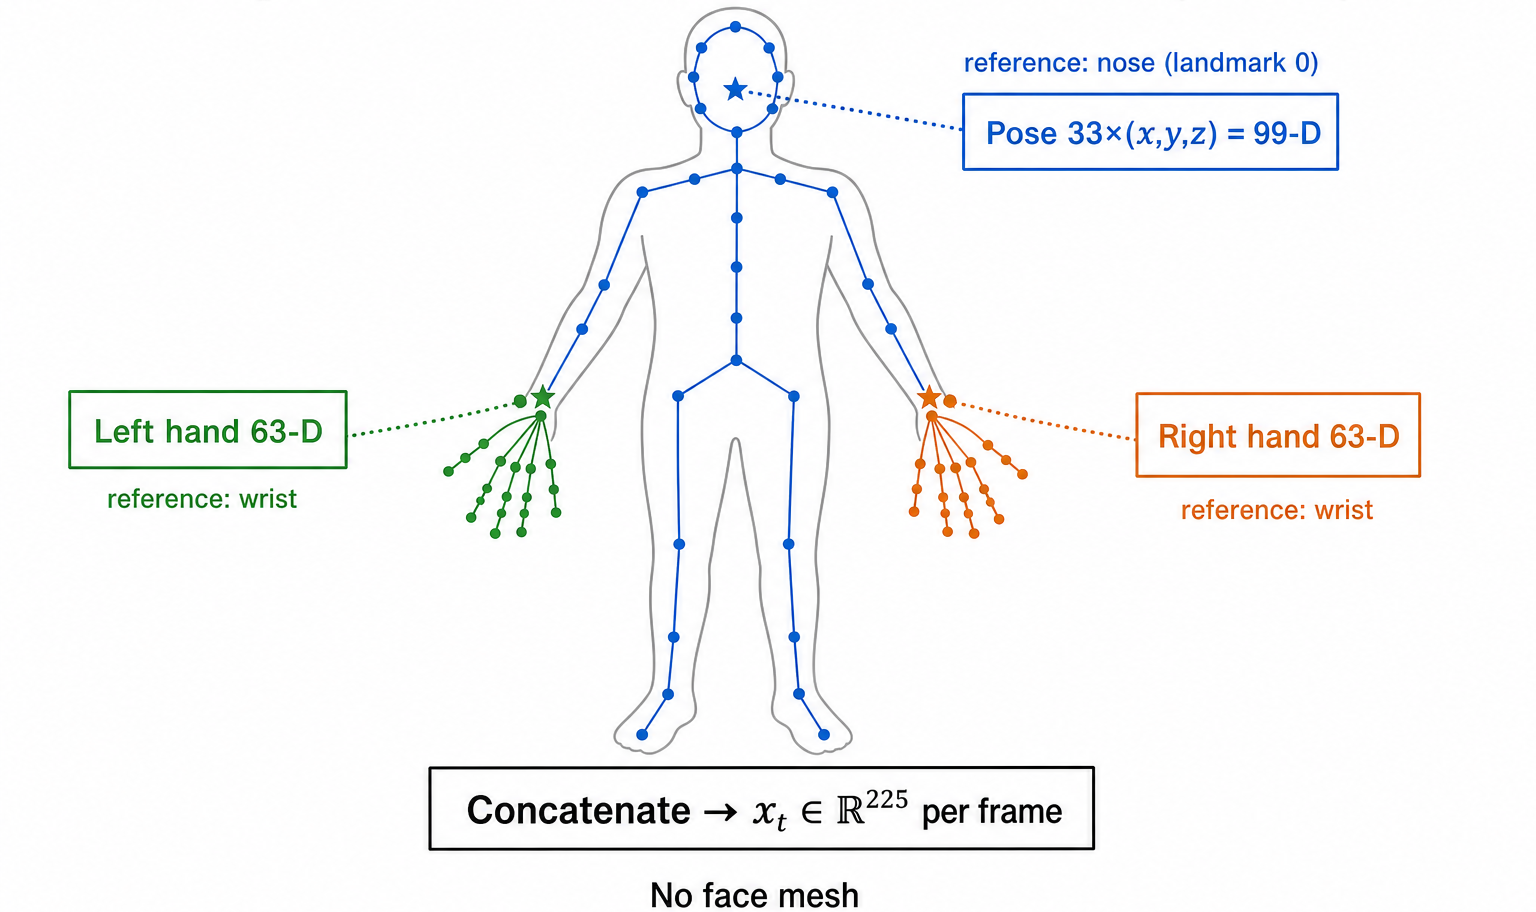
\includegraphics[width=0.99\textwidth]{images/fig_4-4_arsl_holistic_225d.png}
\caption{225-D Holistic feature topology for ArSL words (Model~4). Pose (99-D) is nose-centred; each hand block (63-D) is wrist-centred. No face mesh is included (Table~\ref{tab:ch4-holistic-blocks}).}
\label{fig:ch4-holistic-topology}
\end{figure}
\vspace{0.4cm}

\begin{figure}[H]
\centering
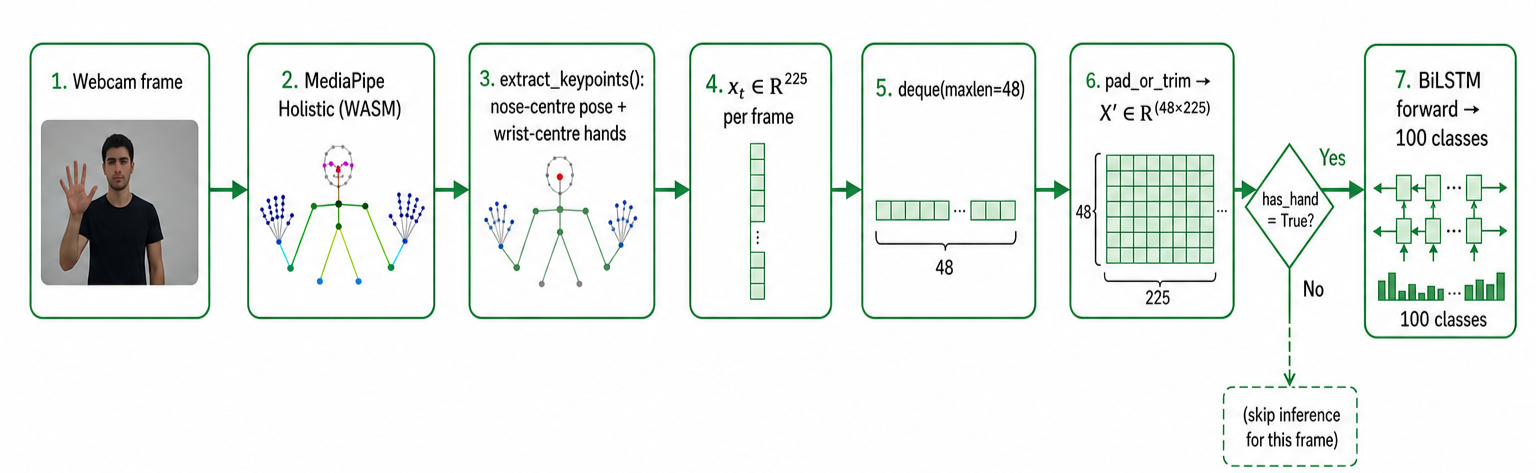
\includegraphics[width=0.99\textwidth]{images/fig_4-5_arsl_holistic_pipeline.png}
\caption{ArSL word Holistic extraction pipeline (Model~4). Landmarks are normalised per frame, buffered to 48 frames, aligned via trim/pad, and classified by the stacked BiLSTM when \texttt{has\_hand} is true (Sections~4.7--4.9).}
\label{fig:ch4-arsl-pipeline}
\end{figure}
\vspace{0.4cm}

\noindent\textbf{4.7.2\quad Body-Relative Normalisation (adjust\_landmarks):}\par
\addcontentsline{toc}{subsection}{\numberline{4.7.2}Body-Relative Normalisation:}
\vspace{0.3cm}

\noindent Each landmark block is centred on a reference joint by subtracting the anchor point $\mathbf{p}_0$ from every $(x,y,z)$ triplet, making the block translation-invariant:
\begin{equation}
\hat{\mathbf{p}}_i^{\text{pose}} = \mathbf{p}_i^{\text{pose}} - \underbrace{\mathbf{p}_0^{\text{pose}}}_{\text{nose}}, \quad i = 0,\ldots,32,
\label{eq:ch4-adjust-pose}
\end{equation}
\begin{equation}
\hat{\mathbf{q}}_j^{\text{hand}} = \mathbf{q}_j^{\text{hand}} - \underbrace{\mathbf{q}_0^{\text{hand}}}_{\text{wrist}}, \quad j = 0,\ldots,20, \quad \text{(left and right hands independently).}
\label{eq:ch4-adjust-hand}
\end{equation}
The three adjusted blocks are flattened and concatenated to form the per-frame feature vector:
\begin{equation}
\mathbf{x}_t = \bigl[\hat{\mathbf{p}}^{\text{pose}}_t;\;\hat{\mathbf{q}}^{\text{lh}}_t;\;\hat{\mathbf{q}}^{\text{rh}}_t\bigr] \in \mathbb{R}^{225}.
\label{eq:ch4-holvec}
\end{equation}
If no pose is detected, $\hat{\mathbf{p}}^{\text{pose}}_t = \mathbf{0}_{99}$; if a hand is absent, the corresponding 63-D block is $\mathbf{0}_{63}$. The live client applies the same zero-fill convention during inference.\par\vspace{0.4cm}

\noindent\textbf{4.7.3\quad Clip Alignment (Trim / Pad):}\par
\addcontentsline{toc}{subsection}{\numberline{4.7.3}Clip Alignment (Trim / Pad):}
\vspace{0.3cm}

\noindent KArSL clip durations vary. Model~4 aligns every sequence to exactly $F{=}48$ frames using trim/pad (Equation~\eqref{eq:ch4-padtrim}):
\begin{equation}
\mathbf{X}' = \begin{cases}
\mathbf{X}[0:48, :] & T_{\text{raw}} \geq 48 \quad\text{(take first 48 frames)}, \\[4pt]
\Bigl[\mathbf{X};\;\underbrace{\mathbf{x}_{T_{\text{raw}}},\ldots,\mathbf{x}_{T_{\text{raw}}}}_{48-T_{\text{raw}}}\Bigr] & T_{\text{raw}} < 48 \quad\text{(repeat last frame)}.
\end{cases}
\label{eq:ch4-padtrim}
\end{equation}
Repeating the final frame retains the end-of-sign body configuration rather than introducing a zero-gap discontinuity. The resulting clip is $\mathbf{X}' \in \mathbb{R}^{48 \times 225}$.\par\vspace{0.4cm}

\begin{figure}[H]
\centering
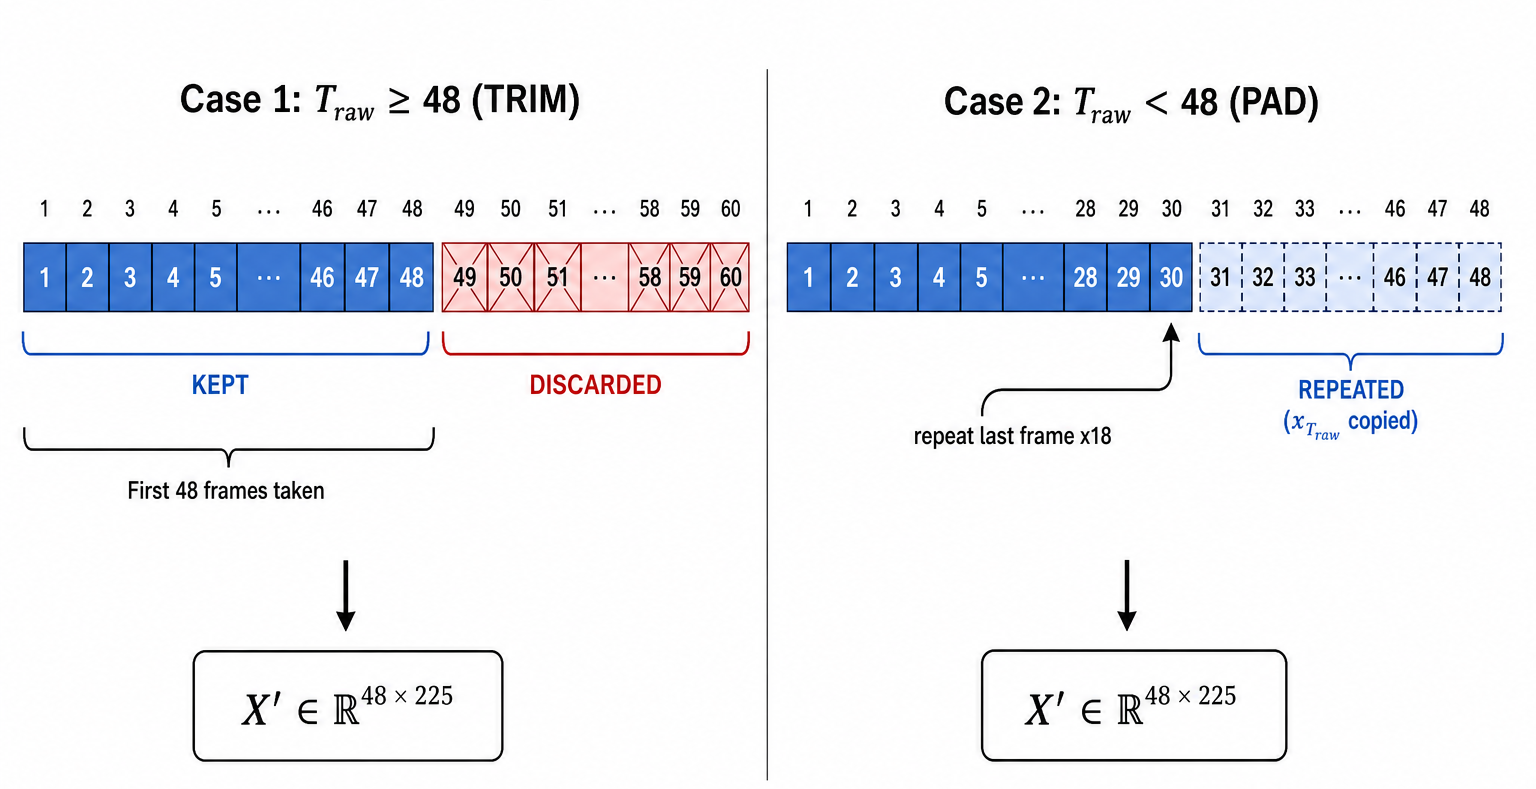
\includegraphics[width=0.99\textwidth]{images/fig_4-10_arsl_padtrim.png}
\caption{Trim/pad clip-alignment policy (Equation~\eqref{eq:ch4-padtrim}). Clips longer than 48 frames are truncated to the first 48; shorter clips are extended by repeating the final body-pose frame until 48 frames are reached. Both cases produce $\mathbf{X}' \in \mathbb{R}^{48 \times 225}$.}
\label{fig:ch4-padtrim}
\end{figure}
\vspace{0.3cm}

\noindent\textbf{No external scaler.} The BiLSTM was trained on raw nose/wrist-centred coordinates (Equations~\eqref{eq:ch4-adjust-pose}--\eqref{eq:ch4-holvec}) without fitting a separate \texttt{StandardScaler}~\cite{pedregosa2011sklearn}. Inference feeds $\mathbf{X}'$ directly into the model without any per-dimension mean/variance correction.\par\vspace{0.6cm}
\clearpage
% --- 4.8 MODEL 4: ArSL BiLSTM ---
\noindent\textbf{4.8\quad MODEL 4 --- ArSL WORD STACKED BiLSTM}\par
\addcontentsline{toc}{section}{\numberline{4.8}MODEL 4 --- ArSL WORD STACKED BiLSTM}
\vspace{0.4cm}

\noindent\textbf{Problem.} Arabic isolated words require two-hand coordination and upper-body motion over 1--2 seconds. The KArSL training set provides only $\sim$50--60 clips per class; a lightweight recurrent model that generalises from compact landmark sequences was therefore preferred over a pixel-intensive 3-D CNN~\cite{sidig2021karsl}.\par\vspace{0.4cm}

\noindent\textbf{4.8.1\quad LSTM Cell Equations:}\par
\addcontentsline{toc}{subsection}{\numberline{4.8.1}LSTM Cell Equations:}
\vspace{0.3cm}

\noindent A single LSTM unit at time step $t$ with input $\mathbf{x}_t \in \mathbb{R}^d$ and previous states $(\mathbf{h}_{t-1}, \mathbf{c}_{t-1}) \in \mathbb{R}^h \times \mathbb{R}^h$ maintains four gated operations~\cite{hochreiter1997long}:
\begin{align}
\mathbf{i}_t &= \sigma(W_i\,\mathbf{x}_t + U_i\,\mathbf{h}_{t-1} + \mathbf{b}_i), \label{eq:ch4-lstm-i} \\
\mathbf{f}_t &= \sigma(W_f\,\mathbf{x}_t + U_f\,\mathbf{h}_{t-1} + \mathbf{b}_f), \label{eq:ch4-lstm-f} \\
\mathbf{o}_t &= \sigma(W_o\,\mathbf{x}_t + U_o\,\mathbf{h}_{t-1} + \mathbf{b}_o), \label{eq:ch4-lstm-o} \\
\tilde{\mathbf{c}}_t &= \tanh(W_c\,\mathbf{x}_t + U_c\,\mathbf{h}_{t-1} + \mathbf{b}_c), \label{eq:ch4-lstm-g} \\
\mathbf{c}_t &= \mathbf{f}_t \odot \mathbf{c}_{t-1} + \mathbf{i}_t \odot \tilde{\mathbf{c}}_t, \label{eq:ch4-lstm-c} \\
\mathbf{h}_t &= \mathbf{o}_t \odot \tanh(\mathbf{c}_t). \label{eq:ch4-lstm-h}
\end{align}
$\sigma$ is sigmoid, $\odot$ is element-wise multiplication. $W_* \in \mathbb{R}^{h \times d}$, $U_* \in \mathbb{R}^{h \times h}$, $\mathbf{b}_* \in \mathbb{R}^h$ are learned parameters. The \textbf{input gate} $\mathbf{i}_t$ writes new content; the \textbf{forget gate} $\mathbf{f}_t$ retains past cell memory; the \textbf{output gate} $\mathbf{o}_t$ exposes the hidden state; the candidate $\tilde{\mathbf{c}}_t$ proposes new cell content. Gating avoids the vanishing-gradient problem over 48-step sequences~\cite{pascanu2013difficulty}.\par\vspace{0.3cm}

\begin{figure}[H]
\centering
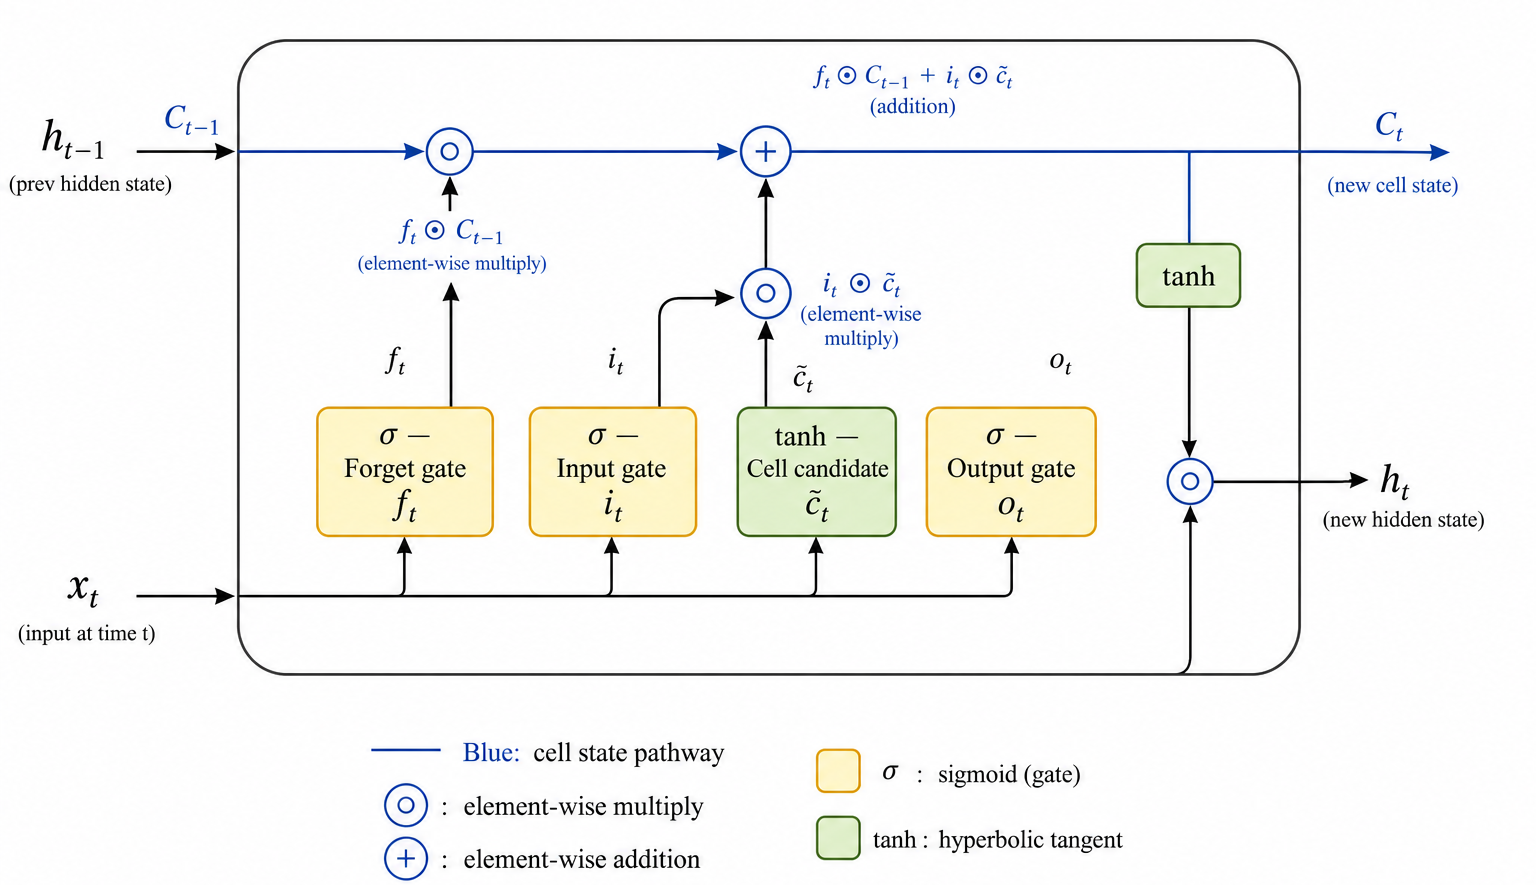
\includegraphics[width=0.99\textwidth]{images/fig_4-11_lstm_cell.png}
\caption{LSTM cell internal structure (Equations~\eqref{eq:ch4-lstm-i}--\eqref{eq:ch4-lstm-h}). The blue cell-state highway $\mathbf{c}_{t-1} \to \mathbf{c}_t$ is gated by the forget gate $\mathbf{f}_t$ (retention) and the input gate $\mathbf{i}_t$ plus candidate $\tilde{\mathbf{c}}_t$ (new content). The output gate $\mathbf{o}_t$ controls how much of $\tanh(\mathbf{c}_t)$ is exposed as the hidden state $\mathbf{h}_t$.}
\label{fig:ch4-lstm-cell}
\end{figure}
\vspace{0.4cm}

\noindent\textbf{4.8.2\quad Bidirectional LSTM:}\par
\addcontentsline{toc}{subsection}{\numberline{4.8.2}Bidirectional LSTM:}
\vspace{0.3cm}

\noindent A BiLSTM runs two independent chains over the sequence --- one forward ($t{=}1\!\to\!T$) and one backward ($t{=}T\!\to\!1$) --- and concatenates both hidden states at every step~\cite{schuster1997bidirectional}:
\begin{equation}
\overrightarrow{\mathbf{h}}_t = \mathrm{LSTM}_{\text{fwd}}(\mathbf{x}_t,\;\overrightarrow{\mathbf{h}}_{t-1}), \qquad \overleftarrow{\mathbf{h}}_t = \mathrm{LSTM}_{\text{bwd}}(\mathbf{x}_t,\;\overleftarrow{\mathbf{h}}_{t+1}),
\label{eq:ch4-bilstm-passes}
\end{equation}
\begin{equation}
\mathbf{h}_t^{\text{bi}} = \bigl[\,\overrightarrow{\mathbf{h}}_t\,;\,\overleftarrow{\mathbf{h}}_t\,\bigr] \in \mathbb{R}^{2h}.
\label{eq:ch4-bilstm-concat}
\end{equation}
Seeing both the sign onset and completion at every time step reduces sensitivity to clip alignment and variable signing speed across signers~\cite{schuster1997bidirectional}.\par\vspace{0.3cm}
\clearpage
\noindent\textbf{4.8.3\quad Full Architecture (Model 4):}\par
\vspace{0.2cm}

\noindent The \texttt{tf.keras.Sequential} model contains exactly four layers:\par\vspace{0.3cm}

\begin{table}[H]
\centering
\caption{ArSL word BiLSTM full architecture (Model~4).}
\label{tab:ch4-bilstm-arch}
\small
\renewcommand{\arraystretch}{1.4} % Adds vertical padding so the text doesn't hit the borders
\begin{tabular}{|c|P{3.8cm}|c|P{2.4cm}|P{4.0cm}|}
\hline
\textbf{Layer \#} & \textbf{Type} & \textbf{Units} & \textbf{Output shape} & \textbf{Notes} \\ \hline
--- & Input & --- & $(48,\;225)$ & $\mathbf{X}' \in \mathbb{R}^{48 \times 225}$ \\ \hline
1 & Bidirectional(LSTM) & 64 & $(48,\;128)$ & \texttt{return\_\allowbreak sequences=True}; concat 64 fwd + 64 bwd \\ \hline
2 & Bidirectional(LSTM) & 64 & $(128)$ & \texttt{return\_\allowbreak sequences=False}; final step only \\ \hline
3 & Dense (ReLU) & 32 & $(32)$ & Affine + ReLU nonlinearity \\ \hline
4 & Dense (Softmax) & 100 & $(100)$ & Class probability distribution \\ \hline
\end{tabular}
\end{table}
\vspace{0.1cm} % Tightened to pull the image up

\begin{figure}[H]
\centering
% Shrunk from 0.72 to 0.65 so it pops back up onto the previous page
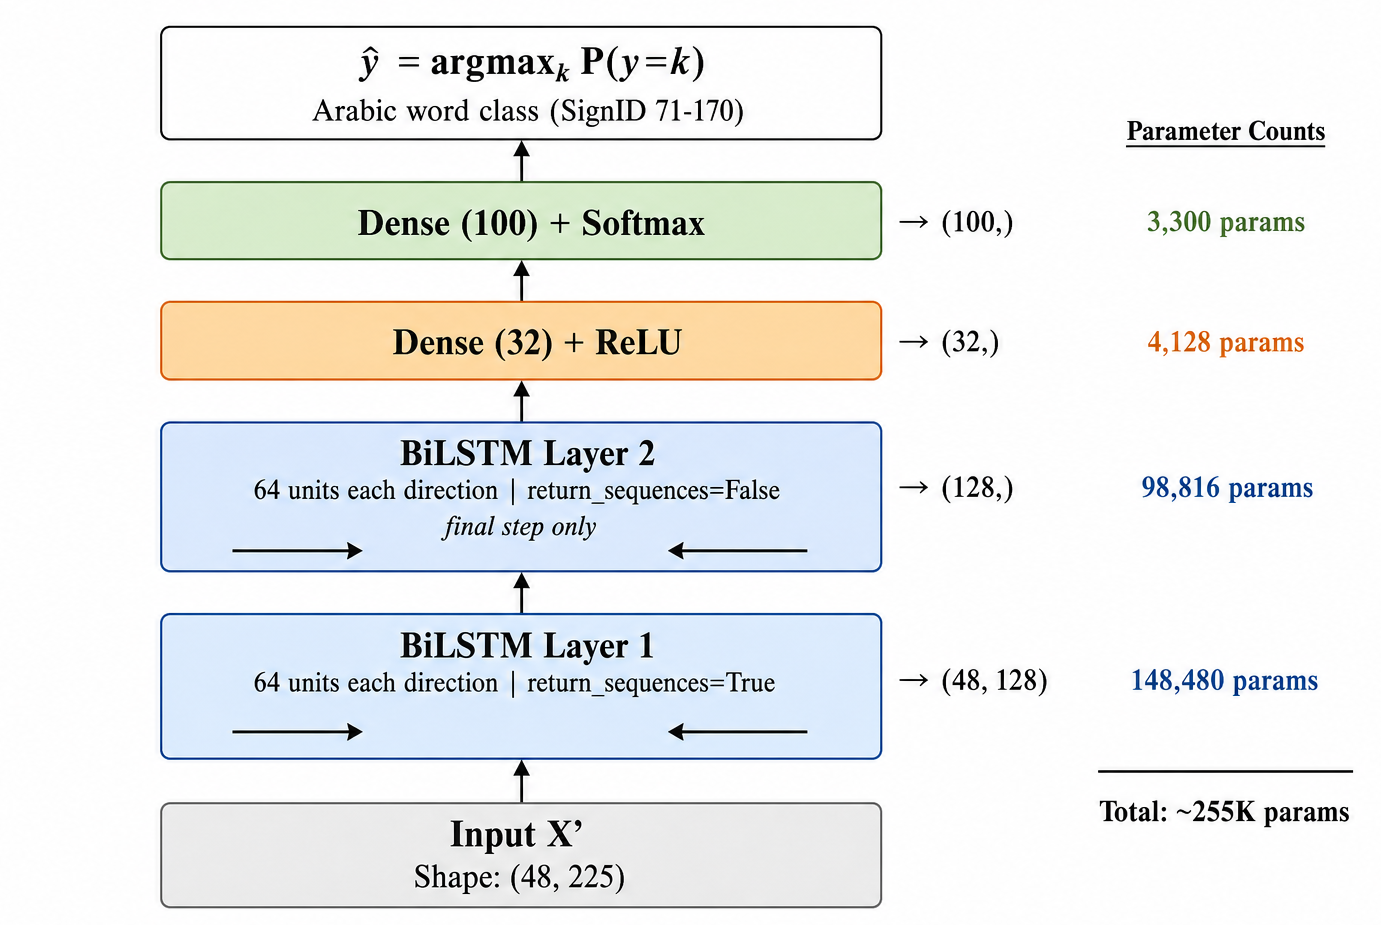
\includegraphics[width=0.71\textwidth]{images/fig_4-12_bilstm_architecture.png}
\caption{ArSL stacked BiLSTM architecture with per-layer output shapes and parameter counts (Table~\ref{tab:ch4-bilstm-arch}). BiLSTM Layer~1 (148\,480 params) returns a per-frame sequence $(48,128)$; Layer~2 (98\,816 params) collapses it to a single 128-D signing summary; Dense(32)+ReLU and Dense(100)+Softmax (7\,428 params total) map to 100 Arabic word class probabilities. Total: $\sim$255\,K parameters.}
\label{fig:ch4-bilstm-arch}
\end{figure}
\vspace{0.4cm}



\noindent\textbf{Forward pass equations.} With input $\mathbf{X}' \in \mathbb{R}^{48 \times 225}$ the four layers compute:
\begin{align}
\mathbf{H}^{(1)} &= \mathrm{BiLSTM}_1\!\bigl(\mathbf{X}',\;h_1{=}64\bigr) \in \mathbb{R}^{48 \times 128}, \label{eq:ch4-L1} \\
\mathbf{h}^{(2)} &= \mathrm{BiLSTM}_2\!\bigl(\mathbf{H}^{(1)},\;h_2{=}64\bigr) \in \mathbb{R}^{128}, \label{eq:ch4-L2} \\
\mathbf{u} &= \mathrm{ReLU}(W_a\,\mathbf{h}^{(2)} + \mathbf{b}_a) \in \mathbb{R}^{32}, \label{eq:ch4-dense1} \\
\mathbf{z} &= W_b\,\mathbf{u} + \mathbf{b}_b \in \mathbb{R}^{100}, \label{eq:ch4-dense2} \\
P(y{=}k \mid \mathbf{X}') &= \frac{\exp(z_k)}{\displaystyle\sum_{j=1}^{100}\exp(z_j)}, \qquad \hat{y} = \arg\max_k P(y{=}k \mid \mathbf{X}'). \label{eq:ch4-bilstm-softmax}
\end{align}

\noindent\textbf{4.8.4\quad Parameter Count:}\par
\addcontentsline{toc}{subsection}{\numberline{4.8.4}Parameter Count:}
\vspace{0.3cm}

\noindent For an LSTM$(h)$ with input $d$, the parameter count per direction is $4(d+h)h + 4h$. Bidirectional doubles this.\par\vspace{0.3cm}

\begin{table}[H]
\centering
\caption{Model~4 parameter breakdown. $d_1{=}225$ (input dim), $h{=}64$ (LSTM units per direction), $d_2{=}128$ (BiLSTM~1 output = $2h$).}
\label{tab:ch4-params}
\small
\begin{tabular}{|P{3.5cm}|P{6.5cm}|r|}
\hline
\textbf{Layer} & \textbf{Formula} & \textbf{Count} \\
\hline
BiLSTM~L1 & $2 \times [4(225+64)\times64 + 4\times64]$ & 148\,480 \\
BiLSTM~L2 & $2 \times [4(128+64)\times64 + 4\times64]$ & 98\,816 \\
Dense(32) & $128\times32 + 32$ & 4\,128 \\
Dense(100) & $32\times100 + 100$ & 3\,300 \\
\hline
\textbf{Total} & & \textbf{254\,724 $\approx$ 255\,K} \\
\hline
\end{tabular}
\end{table}
\vspace{0.4cm}

\noindent The $\sim$255\,K parameter count is two orders of magnitude smaller than the I3D model ($\sim$12.5\,M), reflecting the efficiency of operating on pre-extracted 225-D landmark vectors rather than raw $224\!\times\!224$ RGB frames.\par\vspace{0.3cm}
\clearpage
\noindent\textbf{4.8.5\quad Loss and Training:}\par
\addcontentsline{toc}{subsection}{\numberline{4.8.5}Loss and Training:}
\vspace{0.3cm}

\noindent Training minimises categorical cross-entropy over 100-class one-hot labels:
\begin{equation}
\mathcal{L} = -\sum_{k=1}^{100} y_k \log P(y{=}k \mid \mathbf{X}').
\label{eq:ch4-bilstm-loss}
\end{equation}
Training runs used the software environment in Chapter~3 (Table~\ref{tab:ch3-env}): TensorFlow/Keras on Kaggle GPU for full-sequence extraction and BiLSTM fitting; local 4\,GB CUDA was sufficient for inference prototyping only. The checkpoint filename encodes the converged loss ($\mathcal{L} = 0.026$) and training accuracy (99.625\,\%) at the saved epoch, confirming the model was evaluated on a three-signer held-out partition achieving \textbf{99.62\,\% Top-1 accuracy} on 100 Arabic word classes (SignID 71--170)~\cite{sidig2021karsl}.\par\vspace{0.6cm}

% --- 4.9 ArSL INFERENCE PATH ---
\noindent\textbf{4.9\quad ArSL INFERENCE PATH (End-to-End)}\par
\addcontentsline{toc}{section}{\numberline{4.9}ArSL INFERENCE PATH (END-TO-END)}
\vspace{0.4cm}

\noindent The model-side path from Holistic landmarks to a class probability vector:
\begin{enumerate}
\item MediaPipe Holistic extracts pose and hand landmarks per frame; nose/wrist centreing yields $\mathbf{x}_t \in \mathbb{R}^{225}$ (Equations~\eqref{eq:ch4-adjust-pose}--\eqref{eq:ch4-holvec}).
\item Vectors accumulate in a 48-frame rolling buffer on the client.
\item When the buffer is full and at least one hand is visible, the $(48, 225)$ tensor is forwarded for inference (Chapter~5).
\item The stacked BiLSTM (Equations~\eqref{eq:ch4-L1}--\eqref{eq:ch4-bilstm-softmax}) returns top-$k$ class probabilities.
\end{enumerate}
\vspace{0.3cm}

\noindent Per-request bandwidth is $\approx$43\,KB float32 per 48-frame window ($48 \times 225 \times 4$ bytes), versus several megabytes per second for uncompressed 720p video~\cite{rfc6455}. Deployment artifacts are listed in Table~\ref{tab:ch4-artifacts} (Model~4 row). Results are reported in Chapter~6.\par\vspace{0.6cm}

% ==========================================================
% SHARED SECTIONS
% ==========================================================
\clearpage
% --- 4.10 PIPELINE COMPARISON ---
\noindent\textbf{4.10\quad CROSS-LANGUAGE PIPELINE COMPARISON}\par
\addcontentsline{toc}{section}{\numberline{4.10}CROSS-LANGUAGE PIPELINE COMPARISON}
\vspace{0.4cm}

\noindent The following Table~\ref{tab:ch4-pipeline-compare} contrasts every processing stage of the two word pipelines side by side. Table~\ref{tab:ch4-artifacts} lists the deployment artifacts for both models.\par\vspace{0.2cm}

\begin{table}[H]
\centering
\caption{Detailed cross-language comparison of ASL and ArSL word recognition pipelines.}
\label{tab:ch4-pipeline-compare}
\small
\renewcommand{\arraystretch}{1.2} % Adds vertical padding so the text doesn't hit the borders
\begin{tabular}{|P{3.5cm}|P{5.5cm}|P{5.5cm}|}
\hline
\textbf{Stage} & \textbf{ASL (Model~3 / I3D)} & \textbf{ArSL (Model~4 / BiLSTM)} \\ \hline
Feature source & Raw RGB frames (no MediaPipe) & MediaPipe Holistic (WebAssembly) \\ \hline
Per-frame output & 3$\times$224$\times$224 normalised tensor & 225-D body-relative landmark vector \\ \hline
Normalisation & $(p/255)\times2 - 1 \in [-1,1]$ & Nose-centred pose; wrist-centred hands \\ \hline
Clip / buffer size & 32 frames & 48 frames \\ \hline
Buffer management & \texttt{deque\allowbreak(maxlen=32)}; inference on fill & \texttt{deque\allowbreak(maxlen=48)}; inference if \texttt{has\_hand} \\ \hline
Temporal alignment & Rolling deque (no explicit alignment) & Trim first 48 or repeat-last-frame pad \\ \hline
External scaler & None & None (raw normalised coords) \\ \hline
Model class & Inception I3D (PyTorch) & Stacked BiLSTM (Keras) \\ \hline
Input tensor shape & $(1,3,32,224,224)$ PyTorch & $(1,48,225)$ TensorFlow/Keras \\ \hline
Backbone depth & 19 stages (Table~\ref{tab:ch4-i3d-stack}) & 4 layers (Table~\ref{tab:ch4-bilstm-arch}) \\ \hline
Parameters & $\sim$12.5\,M & $\sim$255\,K \\ \hline
Temporal pooling & Mean of logits over $T_{\text{out}}$ & Final hidden state of BiLSTM~2 \\ \hline
Classification head & 100-class Unit3D ($1\!\times\!1\!\times\!1$) + softmax & Dense(100) + softmax \\ \hline
Stabilisation & Majority vote 6/10, conf$\geq$50\,\%, 1.2\,s & Hand-present gate only \\ \hline
Test Top-1 (100 classes) & \textbf{65.89\,\%} & \textbf{99.62\,\%} \\ \hline
Inference bandwidth & Raw frames encoded (several KB/frame) & $\approx$43\,KB per 48-frame window \\ \hline
\end{tabular}
\end{table}
\vspace{0.4cm}

\begin{table}[H]
\centering
\caption{Deployment artifacts for word recognition (Models~3 and~4).}
\label{tab:ch4-artifacts}
\small
\renewcommand{\arraystretch}{1.8} % Adds vertical padding so the text doesn't hit the borders
\begin{tabular}{|P{2.5cm}|P{5.0cm}|P{6.0cm}|}
\hline
\textbf{Model} & \textbf{Checkpoint / weights} & \textbf{Supporting files} \\ \hline
ASL I3D (M3) & \texttt{asl\_\allowbreak word\_\allowbreak i3d.pt} & 100-class WLASL gloss list \\ \hline
ArSL BiLSTM (M4) & \texttt{arsl\_\allowbreak word\_\allowbreak bilstm.h5} & 100-class Arabic label map (SignID 71--170) \\ \hline
\end{tabular}
\end{table}
\vspace{0.4cm}

\begin{figure}[H]
\centering
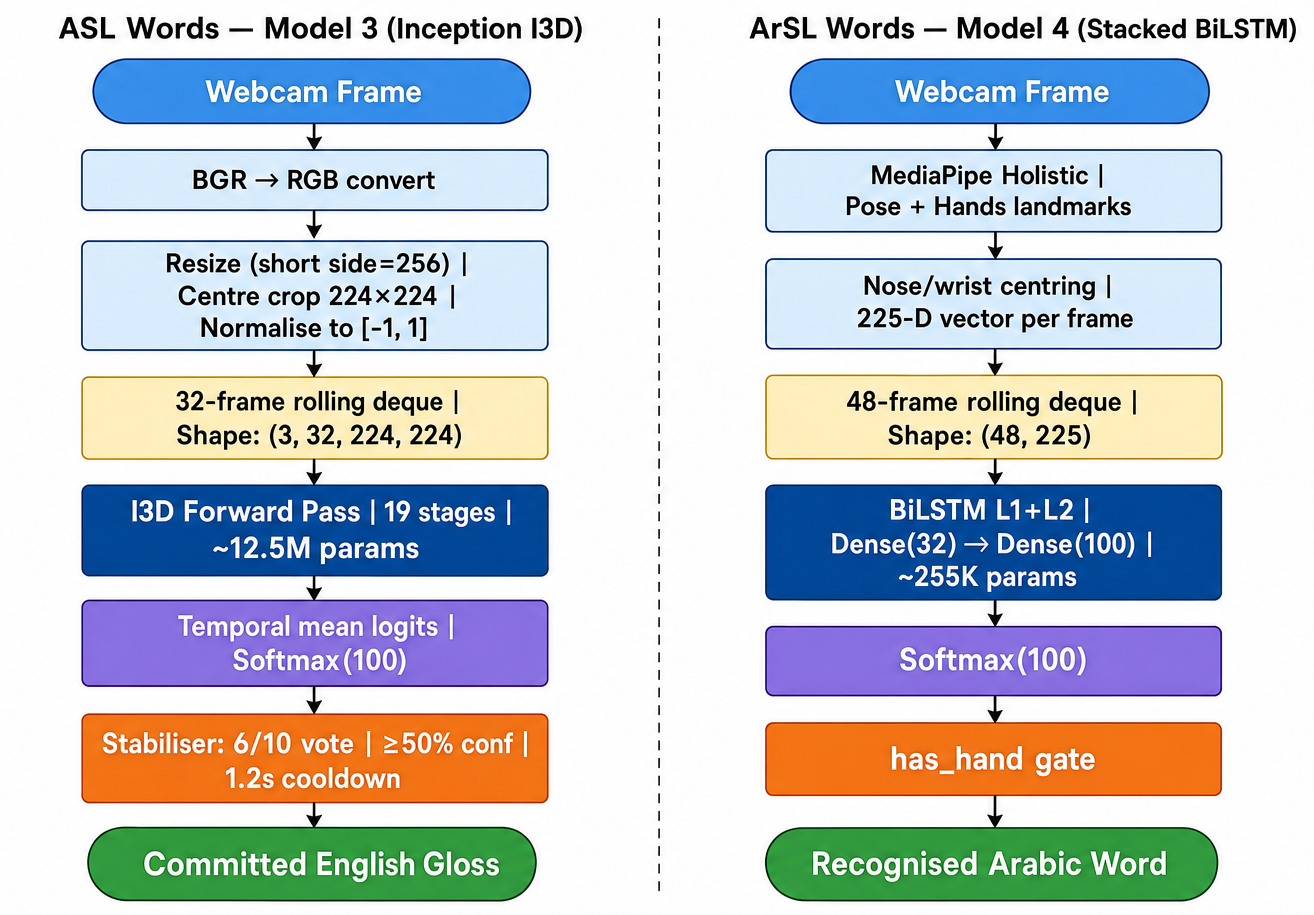
\includegraphics[width=0.99\textwidth]{images/fig_4-13_pipeline_sidebyside.png}
\caption{Side-by-side word inference pipelines for ASL (Model~3, Inception I3D, left) and ArSL (Model~4, Stacked BiLSTM, right). Both pipelines share a rolling-deque temporal buffer and a 100-class softmax output, but differ in feature source (RGB pixels vs.\ Holistic landmarks), buffer depth (32 vs.\ 48 frames), model architecture, parameter count, and stabilisation strategy. See Table~\ref{tab:ch4-pipeline-compare} for a detailed comparison.}
\label{fig:ch4-side-by-side}
\end{figure}
\vspace{0.6cm}
% --- 4.11 TRADE-OFFS ---
\clearpage
\noindent\textbf{4.11\quad ENGINEERING TRADE-OFFS}\par
\addcontentsline{toc}{section}{\numberline{4.11}ENGINEERING TRADE-OFFS}
\vspace{0.4cm}

\noindent Deploying deep neural networks to a live, web-based environment requires carefully balancing theoretical offline accuracy against real-time physical constraints, such as inference latency, memory footprint, and the end user's hardware limitations. Table~\ref{tab:ch4-tradeoffs-asl} records the ASL-specific decisions, where computational cost was traded for the robust spatio-temporal feature extraction of I3D. Conversely, Table~\ref{tab:ch4-tradeoffs-arsl} records the ArSL-specific decisions, which prioritised a lightweight, landmark-based sequence approach suitable for a highly constrained, smaller dataset.\par\vspace{0.4cm}

\begin{table}[H]
\centering
\caption{Engineering trade-offs for ASL word recognition (Model~3).}
\label{tab:ch4-tradeoffs-asl}
\small
\renewcommand{\arraystretch}{1.6} % Adds vertical padding so the text doesn't hit the borders
\begin{tabular}{|P{3.0cm}|P{3.2cm}|P{6.6cm}|}
\hline
\textbf{Decision} & \textbf{Alternative considered} & \textbf{Rationale} \\ \hline
Pretrained I3D (\texttt{asl\_\allowbreak word\_\allowbreak i3d.pt}) & Train BiLSTM+attention from scratch & 4\,GB local GPU; I3D captures spatio-temporal pixel appearance without manual landmark engineering \\ \hline
100-class WLASL subset & Larger offline Holistic experiment & Pretrained I3D is Eshara's deployed ASL word model \\ \hline
Majority vote (6/10) + confidence (50\,\%) & Raw top-1 per clip & Suppresses per-clip noise from mid-gesture frames \\ \hline
1.2\,s cooldown between commits & No cooldown & Prevents the same word triggering twice from a slow signing motion \\ \hline
32-frame deque (not longer) & 64-frame window & Shorter window matches WLASL signing speed and reduces commit latency \\ \hline
\end{tabular}
\end{table}
\vspace{0.4cm}

\begin{table}[H]
\centering
\caption{Engineering trade-offs for ArSL word recognition (Model~4).}
\label{tab:ch4-tradeoffs-arsl}
\small
\renewcommand{\arraystretch}{1.5}
\begin{tabular}{|P{3.0cm}|P{3.2cm}|P{6.6cm}|}
\hline
\textbf{Decision} & \textbf{Alternative considered} & \textbf{Rationale} \\ \hline
Stacked BiLSTM ($\sim$255\,K) & Transformer / full self-attention & $\sim$50 clips/class; BiLSTM generalises reliably with far fewer parameters \\ \hline
225-D nose/wrist-normalised Holistic & Unnormalised pose+hands & Body-relative normalisation reduces camera-distance and signer-height sensitivity \\ \hline
Trim first 48 / repeat-last-frame pad & Uniform temporal resampling & Preserves natural sign endpoints; avoids motion artefacts from frame interpolation \\ \hline
No external scaler & StandardScaler (mean/std per dim) & Model trained on raw normalised coordinates; scaler not saved with checkpoint \\ \hline
48-frame window (vs.\ 32-frame ASL) & Same window for both languages & Average KArSL Arabic word sign is longer than average WLASL English clip~\cite{sidig2021karsl} \\ \hline
100-class KArSL (SignID 71--170) & Full 502-class KArSL & Sample density per class; graduation vocabulary scope \\ \hline
Hand-present gate (\texttt{has\_\allowbreak hand}) & Run inference every frame & Prevents committing on empty frames where no hands are visible \\ \hline
\end{tabular}
\end{table}
\vspace{0.6cm}

% --- 4.12 EVALUATION ---
\noindent\textbf{4.12\quad EVALUATION PROTOCOL (WORDS)}\par
\addcontentsline{toc}{section}{\numberline{4.12}EVALUATION PROTOCOL (WORDS)}
\vspace{0.4cm}

\noindent Each word model is evaluated on a \textbf{held-out test partition} explicitly reserved from the training process or hyperparameter selection phase. Because sign language datasets often suffer from severe class imbalance---where common signs possess significantly more video samples than rare ones---relying solely on Top-1 accuracy can provide a misleading estimate of real-world reliability. Therefore, the evaluation protocol incorporates Top-5 accuracy and Macro-F1 scores to ensure a holistic view of the models' predictive power across all classes, including scarce ones. Table~\ref{tab:ch4-eval-protocol} maps each metric to both models; numeric results appear in Chapter~6~\cite{li2020wlasl,sidig2021karsl,powers2011evaluation}.\par\vspace{0.4cm}

\begin{table}[H]
\centering
\caption{Word-model evaluation protocol (reported in Chapter~6).}
\label{tab:ch4-eval-protocol}
\small
\renewcommand{\arraystretch}{1.6}
\begin{tabular}{|P{3.4cm}|P{5.2cm}|P{5.2cm}|}
\hline
\textbf{Metric} & \textbf{ASL I3D (Model~3)} & \textbf{ArSL BiLSTM (Model~4)} \\ \hline
Top-1 accuracy & WLASL 100-class held-out test & KArSL SignID 71--170 held-out test \\ \hline
Top-5 accuracy & Same test partition & Same test partition \\ \hline
Macro-F1 & Class-balanced summary & Class-balanced summary \\ \hline
Weighted-F1 & Optional secondary metric & Optional secondary metric \\ \hline
Confusion matrix & Per-gloss error analysis & Per-class error analysis \\ \hline
Per-class F1 & Scarce-class diagnosis & Scarce-class diagnosis \\ \hline
End-to-end latency & Live web path (Section~5.12) & Live web path (Section~5.12) \\ \hline
\end{tabular}
\end{table}
\vspace{0.3cm}

\noindent\textbf{ASL word rule:} Top-1 and Top-5 for Model~3 are measured exclusively on the WLASL 100-class held-out test set to ensure no data leakage occurs from the training clips (Chapter~6)~\cite{li2020wlasl}.\par\vspace{0.3cm}

\noindent\textbf{ArSL word rule:} The 99.62\,\% Top-1 metric encoded in the checkpoint filename is derived from the three-signer held-out partition at training time. The full thesis evaluation on KArSL SignID 71--170 test clips rigorously uses the exact preprocessing pipeline established in Sections~4.7.1--4.7.3 (Chapter~6)~\cite{sidig2021karsl}.\par\vspace{0.4cm}

\noindent\textbf{Chapter summary.} \textbf{Part~A (Model~3):} pretrained Inception I3D ($\sim$12.5\,M params) on 32-frame $224\!\times\!224$ RGB clips with majority-vote stabilisation (Tables~\ref{tab:ch4-i3d-stack}, \ref{tab:ch4-stab-params}). \textbf{Part~B (Model~4):} stacked BiLSTM ($\sim$255\,K params) on 48-frame 225-D Holistic sequences for 100 Arabic word classes (Tables~\ref{tab:ch4-bilstm-arch}, \ref{tab:ch4-tradeoffs-arsl}; 99.62\,\% Top-1). Shared deployment artifacts and evaluation protocol are in Tables~\ref{tab:ch4-artifacts} and~\ref{tab:ch4-eval-protocol}. Chapter~6 reports offline accuracy; Chapter~5 reports live web latency.\par

\clearpage
\newpage
% ==========================================
%              CHAPTER FIVE
% ==========================================
\thispagestyle{plain}

\begin{center}
    \vspace*{0.5cm}
    {\large \textit{Chapter Five}} \\[0.4cm]
    {\Large \textbf{5 \quad SYSTEM IMPLEMENTATION}}
\end{center}
\addcontentsline{toc}{chapter}{\textbf{5 \quad SYSTEM IMPLEMENTATION}}
\vspace{0.45in}

\normalsize
\startchapterfloats{5}

% Framed screenshot placeholder: swap for \includegraphics when the
% screenshot is ready. #1 = box height, #2 = description shown in box.
\newcommand{\imgplaceholder}[2]{%
  \fbox{\parbox[c][#1][c]{0.92\textwidth}{\centering
    \textbf{[INSERT IMAGE]}\\[4pt] \small #2}}}

\noindent Chapters~3--4 detailed the design, feature engineering, and architecture of the four standalone recognition models. This chapter documents how those models are wrapped into \textbf{Eshara}, a deployable web application, and describes the surrounding product engineering: architecture, frontend, backend, database, real-time communication, security, and testing. The web application is the primary interface through which a user reaches the underlying deep-learning models for American Sign Language (ASL) and Arabic Sign Language (ArSL); it processes standard webcam input directly in the browser, requiring no dedicated hardware or native application install~\cite{fastapi,react,vite2024}. Graduation deployment scope is \textbf{web-only} --- no native mobile application, sensor gloves, or depth cameras~\cite{typescript2024}. The chapter is presented in two parts: \textbf{Part~A} (Sections~5.1--5.13) documents the core application --- system architecture, frontend, backend, database, translation workflow, security, deployment, and measured performance; \textbf{Part~B} (Section~5.14) documents the \textbf{Education Module} --- the bilingual Sign Viewer, Sentence Builder, and Practice tools built on motion-capture skeleton playback --- at the same technical depth.\par\vspace{0.3cm}

\begin{center}{\large \textbf{PART A --- CORE APPLICATION}}\end{center}
\vspace{0.1cm}

\noindent\textbf{5.1\quad SYSTEM ARCHITECTURE}\par
\addcontentsline{toc}{section}{\numberline{5.1}SYSTEM ARCHITECTURE}
\vspace{0.2cm}

\noindent Eshara adopts a \textbf{decoupled, three-tier architecture} so that computationally heavy machine-learning inference does not interfere with the responsiveness of the user interface or the core backend services:
\begin{enumerate}
\item \textbf{Client Tier (Frontend)} --- a responsive interface built with React and bundled with Vite~\cite{react,vite2024}, responsible for capturing the user's webcam stream and drawing educational stickman animations. It communicates with the backend over RESTful APIs for translation requests and over Socket.IO for real-time chat~\cite{socketio2024}.
\item \textbf{Application Tier (Backend API)} --- a Node.js and Express application~\cite{nodejs2024,expressjs2024} that acts as the secure gateway: it manages user authentication (JSON Web Tokens), session state, and database access through the Prisma ORM~\cite{prisma2024,rfc7519}, and proxies \texttt{/predict} requests from the client to the internal model service, hiding the ML environment from the public-facing client.
\item \textbf{Inference Tier (Model Services)} --- a dedicated FastAPI (Python) service~\cite{fastapi,uvicorn2024} that hosts the standalone translation models behind a single \texttt{/predict} endpoint, decodes base64-encoded frames or MediaPipe landmark vectors, and returns predicted text with a confidence score. It also manages generation and serving of \texttt{.pose} files consumed by the frontend's full-body word-sign visualisation.
\end{enumerate}
\vspace{0.2cm}

\noindent \textbf{Data-flow summary.} The user's webcam feed is sampled on the client as a base64-encoded JPEG and sent via an HTTP \texttt{POST} to the Application Tier. The Node.js server authenticates the request and forwards the payload internally to the Inference Tier. FastAPI runs the model appropriate to the requested language/mode combination (MLP for letters, BiLSTM or I3D for words) and the resulting prediction is propagated back through Node.js to the React interface in real time.\par\vspace{0.2cm}

\begin{figure}[H]
\centering
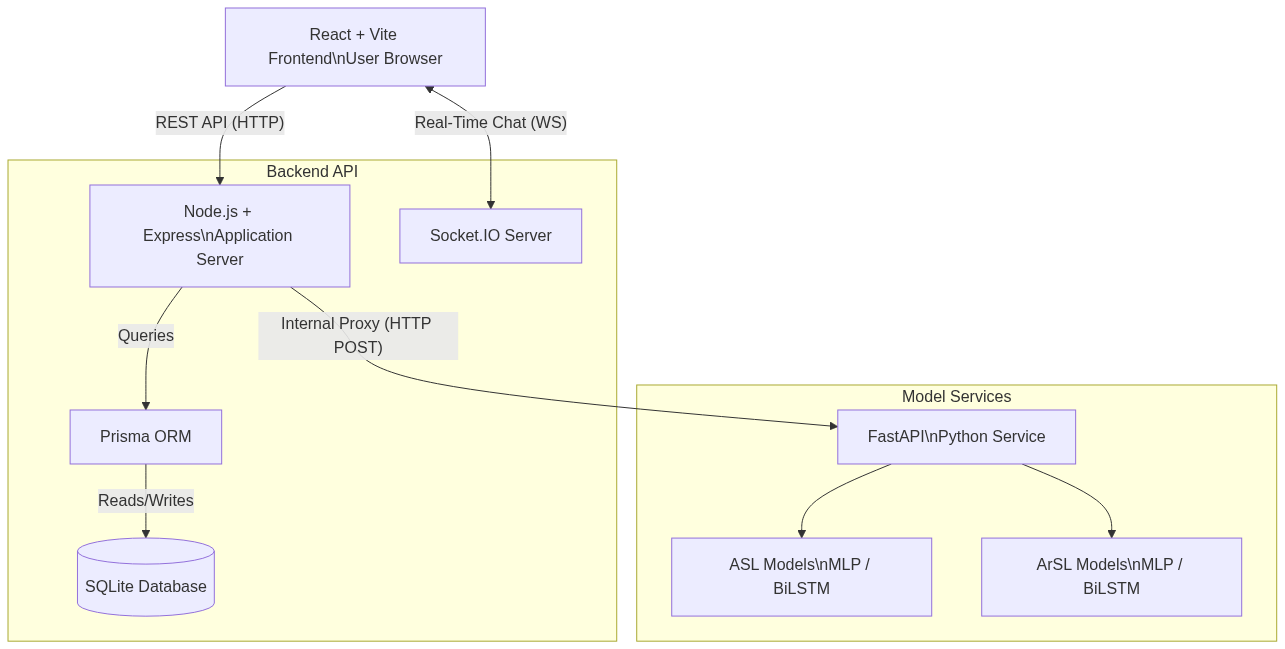
\includegraphics[width=1.00\textwidth]{images/fig_7-1_system_architecture.png}
\caption{Eshara three-tier system architecture: React/Vite client, Node.js + Express application server (Prisma ORM over SQLite, Socket.IO server), and the FastAPI model-services tier hosting the ASL/ArSL letter and word models.}
\label{fig:ch7-architecture}
\end{figure}
\vspace{0.2cm}

\noindent Within this deployment topology, the client only ever talks to the Node.js application server; the FastAPI inference tier is not exposed to the public internet, which both simplifies the client's networking surface and centralises CORS and validation policy in one place (Section~5.10).\par\vspace{0.2cm}

\begin{figure}[H]
\centering
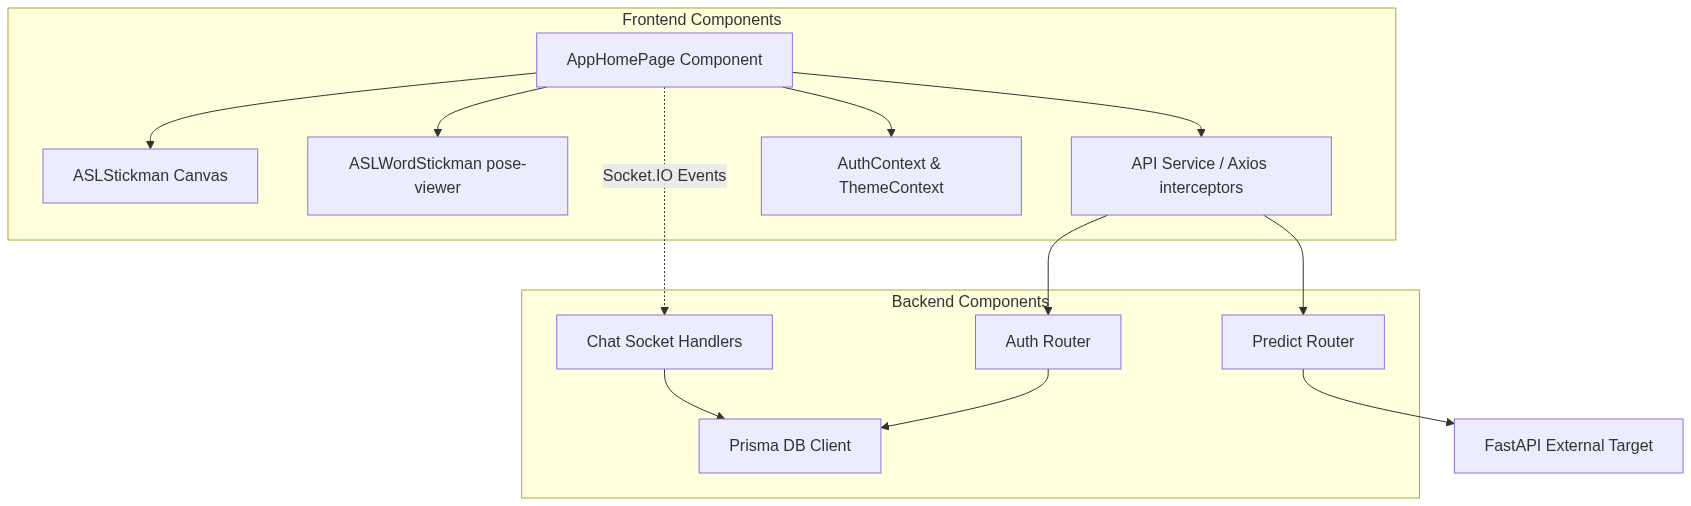
\includegraphics[width=1.00\textwidth]{images/fig_7-2_component_diagram.png}
\caption{Component diagram: frontend modules (\texttt{AppHomePage}, stickman/\texttt{pose-viewer} visualisers, \texttt{AuthContext}/\texttt{ThemeContext}, Axios service layer) and their dependencies on backend components (chat socket handlers, auth router, predict router, Prisma client, and the external FastAPI target).}
\label{fig:ch7-component}
\end{figure}
\vspace{0.3cm}

\noindent\textbf{5.2\quad FRONTEND DESIGN}\par
\addcontentsline{toc}{section}{\numberline{5.2}FRONTEND DESIGN}
\vspace{0.2cm}

\noindent The client is a Single Page Application (SPA) built with React and bundled by Vite for fast hot-module replacement and optimised delivery. The design methodology centres on reusable components, centralised state management, and a lightweight vanilla styling system rather than a heavy CSS framework.\par\vspace{0.2cm}

\noindent\textbf{5.2.1\quad State and component architecture:}\par
\addcontentsline{toc}{subsection}{\numberline{5.2.1}State and component architecture:}
\vspace{0.2cm}

\noindent Global application state --- user authentication sessions and UI theme preference --- is managed through React Context (\texttt{AuthContext} and \texttt{ThemeContext}), avoiding prop-drilling and keeping the UI synchronised across views. Main pages (\texttt{LandingPage}, \texttt{AppHomePage}) handle routing and high-level logic, while discrete components such as \texttt{ASLWordStickman} (the Sign Viewer), \texttt{SentenceBuilder}, and \texttt{PracticePanel} encapsulate the more complex playback and capture logic.\par\vspace{0.2cm}

\noindent\textbf{5.2.2\quad Styling and theming:}\par
\addcontentsline{toc}{subsection}{\numberline{5.2.2}Styling and theming:}
\vspace{0.2cm}

\noindent The application uses vanilla CSS (\texttt{index.css}) with CSS custom properties to define a shared design system for colours, gradients, and typography (Outfit font family), avoiding the overhead of a component-styling framework. A root-level \texttt{data-theme} attribute is toggled dynamically to switch between a dark mode and a high-contrast light mode, supporting usability under varying lighting conditions.\par\vspace{0.2cm}

\clearpage
\noindent\textbf{5.2.3\quad Education module interface:}\par
\addcontentsline{toc}{subsection}{\numberline{5.2.3}Education module interface:}
\vspace{0.2cm}

\noindent A core feature of the frontend is the \textbf{Educational} interface, which teaches sign language through two complementary mechanisms:
\begin{itemize}
\item \textbf{Sign playback (\texttt{<pose-viewer>})} --- all word signs, fingerspelling, and free-text sentences render as motion-capture skeleton animations of real signers, assembled server-side by the model-services tier and played by the \texttt{<pose-viewer>} web component~\cite{signmt2023,poseformat}.
\item \textbf{Practice capture (\texttt{useCamera})} --- a webcam practice panel reuses the same capture-and-\texttt{/predict} pipeline as the Chatting tab through a shared \texttt{useCamera} hook, with its own camera instance so the two tabs never interfere.
\end{itemize}
The module's full architecture --- content pipeline, server-side animation stitching, bilingual behaviour, and verification methodology --- is documented in Section~5.14 (Part~B).
\vspace{0.2cm}

\noindent\textbf{5.2.4\quad Webcam capture and layout:}\par
\addcontentsline{toc}{subsection}{\numberline{5.2.4}Webcam capture and layout:}
\vspace{0.2cm}

\noindent A responsive grid layout houses the live translation interface, which interacts with the browser's \texttt{navigator.mediaDevices} API~\cite{w3c2023html} to let the user select a specific camera input. The video stream is drawn to a horizontally inverted \texttt{<video>} element, acting as a mirror so the user receives intuitive visual feedback before a frame is sampled and sent to the backend.\par\vspace{0.3cm}

\noindent\textbf{5.3\quad BACKEND INTEGRATION AND AUTHENTICATION}\par
\addcontentsline{toc}{section}{\numberline{5.3}BACKEND INTEGRATION AND AUTHENTICATION}
\vspace{0.2cm}

\noindent\textbf{5.3.1\quad Core application server:}\par
\addcontentsline{toc}{subsection}{\numberline{5.3.1}Core application server:}
\vspace{0.2cm}

\noindent The backend is built with Node.js and Express~\cite{nodejs2024,expressjs2024} and acts as the central middleware and routing layer. Modular Express routers expose RESTful endpoints (\texttt{/auth}, \texttt{/users}, \texttt{/predict}, \texttt{/health}), keeping route concerns cleanly separated. To encapsulate the ML environment, the \texttt{predict} controller receives prediction requests (base64 image payloads, requested language and mode) and proxies them asynchronously to the internal FastAPI service, which hides the ML application's network ports from the public client and centralises CORS and validation policy in the Node.js layer.\par\vspace{0.2cm}

\noindent\textbf{5.3.2\quad Authentication infrastructure:}\par
\addcontentsline{toc}{subsection}{\numberline{5.3.2}Authentication infrastructure:}
\vspace{0.2cm}

\noindent Authentication is stateless and based on JSON Web Tokens~\cite{rfc7519}. On registration and login, passwords are hashed with \texttt{bcryptjs} using a high salt-round count before database insertion~\cite{bcrypt2024}; on successful authentication the server issues a cryptographically signed JWT payload carrying the user's ID and email. The React client stores this token and injects it as an \texttt{Authorization: Bearer} header on every outbound request via a custom Axios interceptor~\cite{axios2024}; a \texttt{401 Unauthorized} response causes the interceptor to purge the local token and route the user back to the login gateway.\par\vspace{0.2cm}
\clearpage
\noindent\textbf{5.3.3\quad Real-time communication (Socket.IO):}\par
\addcontentsline{toc}{subsection}{\numberline{5.3.3}Real-time communication (Socket.IO):}
\vspace{0.2cm}

\noindent Live chat and messaging use a Socket.IO server~\cite{socketio2024} layered over the core HTTP instance. The connection handshake is intercepted to validate the JWT before a socket is admitted, immediately dropping unauthorised connections and preventing access to private room broadcasts. Custom event emitters (\texttt{chat:join}, \texttt{chat:send}, \texttt{chat:receive}) deliver messages and UI updates instantaneously, avoiding the latency and overhead of HTTP polling.\par\vspace{0.3cm}

\noindent\textbf{5.4\quad DATABASE DESIGN}\par
\addcontentsline{toc}{section}{\numberline{5.4}DATABASE DESIGN}
\vspace{0.2cm}

\noindent\textbf{5.4.1\quad Prisma ORM and SQLite:}\par
\addcontentsline{toc}{subsection}{\numberline{5.4.1}Prisma ORM and SQLite:}
\vspace{0.2cm}

\noindent Persistence uses the Prisma ORM~\cite{prisma2024} paired with an SQLite database~\cite{sqlite2024}, giving an auto-generated, type-safe database client and rapid schema iteration without the overhead of running a standalone database server. The schema (\texttt{schema.prisma}) defines four models --- \texttt{User}, \texttt{Room}, \texttt{RoomMember}, and \texttt{Message} --- with strict foreign-key constraints and cascading deletes, so that deleting a room automatically removes its associated memberships and messages rather than leaving orphaned rows.\par\vspace{0.2cm}

\begin{figure}[H]
\centering
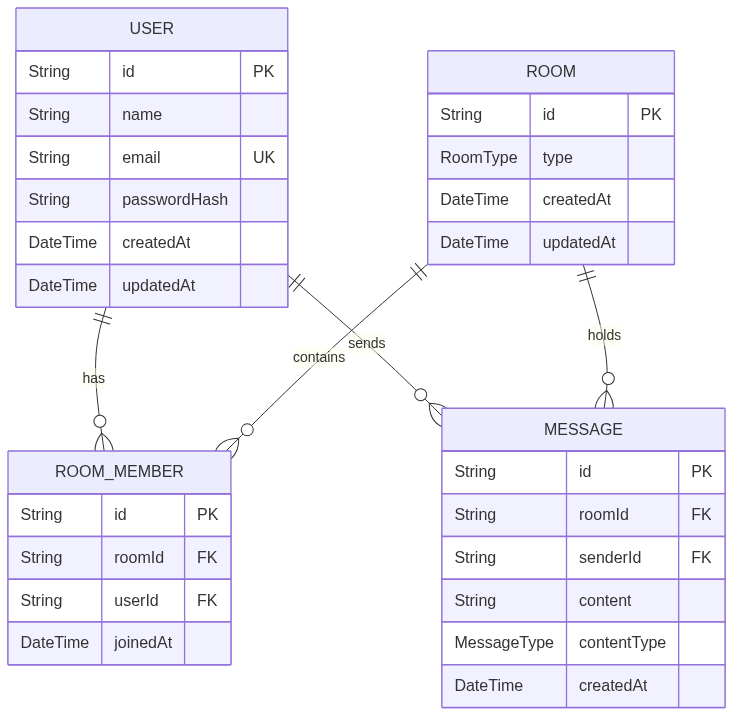
\includegraphics[width=0.95\textwidth]{images/fig_7-4_erd.png}
\caption{Entity--Relationship Diagram (ERD): \texttt{User}, \texttt{Room}, \texttt{ROOM\_MEMBER}, and \texttt{MESSAGE} tables with primary/foreign keys and cascading relationships, as defined in \texttt{schema.prisma}.}
\label{fig:ch7-erd}
\end{figure}
\vspace{0.2cm}

\noindent\textbf{5.4.2\quad Chat and message models:}\par
\addcontentsline{toc}{subsection}{\numberline{5.4.2}Chat and message models:}
\vspace{0.2cm}

\noindent A \texttt{RoomType} enumeration (\texttt{DIRECT} vs.\ \texttt{GROUP}) supports both one-to-one and multi-user chat configurations. The \texttt{Message} model additionally carries a \texttt{MessageType} enumeration (\texttt{TEXT}, \texttt{PREDICTION}, \texttt{SYSTEM}), letting the frontend distinguish manually typed text from strings produced by the AI translation engine and style them differently in the chat UI.\par\vspace{0.2cm}

\begin{figure}[H]
\centering
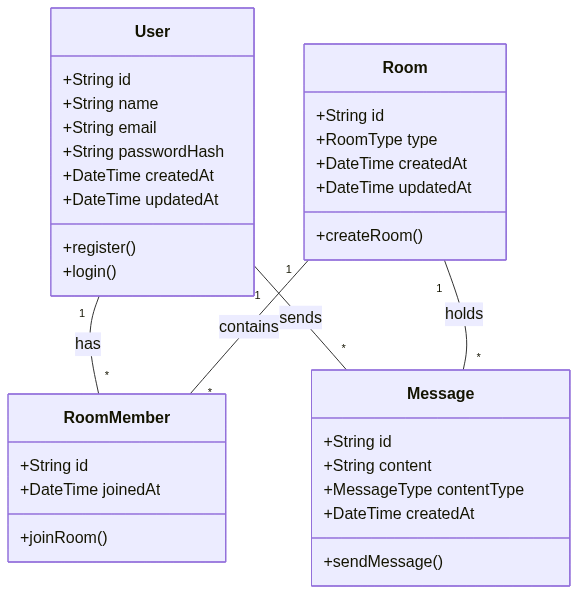
\includegraphics[width=0.95\textwidth]{images/fig_7-5_class_diagram.png}
\caption{Class diagram of the application-server domain objects (\texttt{User}, \texttt{Room}, \texttt{RoomMember}, \texttt{Message}) and their principal operations (\texttt{register()}, \texttt{login()}, \texttt{createRoom()}, \texttt{joinRoom()}, \texttt{sendMessage()}).}
\label{fig:ch7-class}
\end{figure}
\vspace{0.3cm}

\clearpage

\noindent\textbf{5.5\quad TRANSLATION WORKFLOW AND AI MODEL COMMUNICATION}\par
\addcontentsline{toc}{section}{\numberline{5.5}TRANSLATION WORKFLOW AND AI MODEL COMMUNICATION}
\vspace{0.2cm}

\noindent\textbf{5.5.1\quad Image capture and encoding:}\par
\addcontentsline{toc}{subsection}{\numberline{5.5.1}Image capture and encoding:}
\vspace{0.2cm}

\noindent The inference workflow begins on the React frontend: when the user requests a translation, a frame is synchronously captured from the active \texttt{<video>} element, drawn onto a hidden \texttt{<canvas>}, and encoded as a JPEG base64 string. This compression reduces payload size while preserving enough pixel detail for accurate landmark extraction downstream.\par\vspace{0.2cm}

\noindent\textbf{5.5.2\quad Cross-service communication:}\par
\addcontentsline{toc}{subsection}{\numberline{5.5.2}Cross-service communication:}
\vspace{0.2cm}

\noindent The encoded base64 string, together with the user's selected configuration metadata (language: ASL/ArSL; mode: letters/words), is dispatched to the Node.js \texttt{/predict} endpoint. The server authenticates the JWT and, on success, proxies the payload directly to the FastAPI model service over an internal HTTP request, acting as a secure intermediary that keeps the ML service address out of client-visible network traffic.\par\vspace{0.2cm}
\begin{figure}[H]
\centering
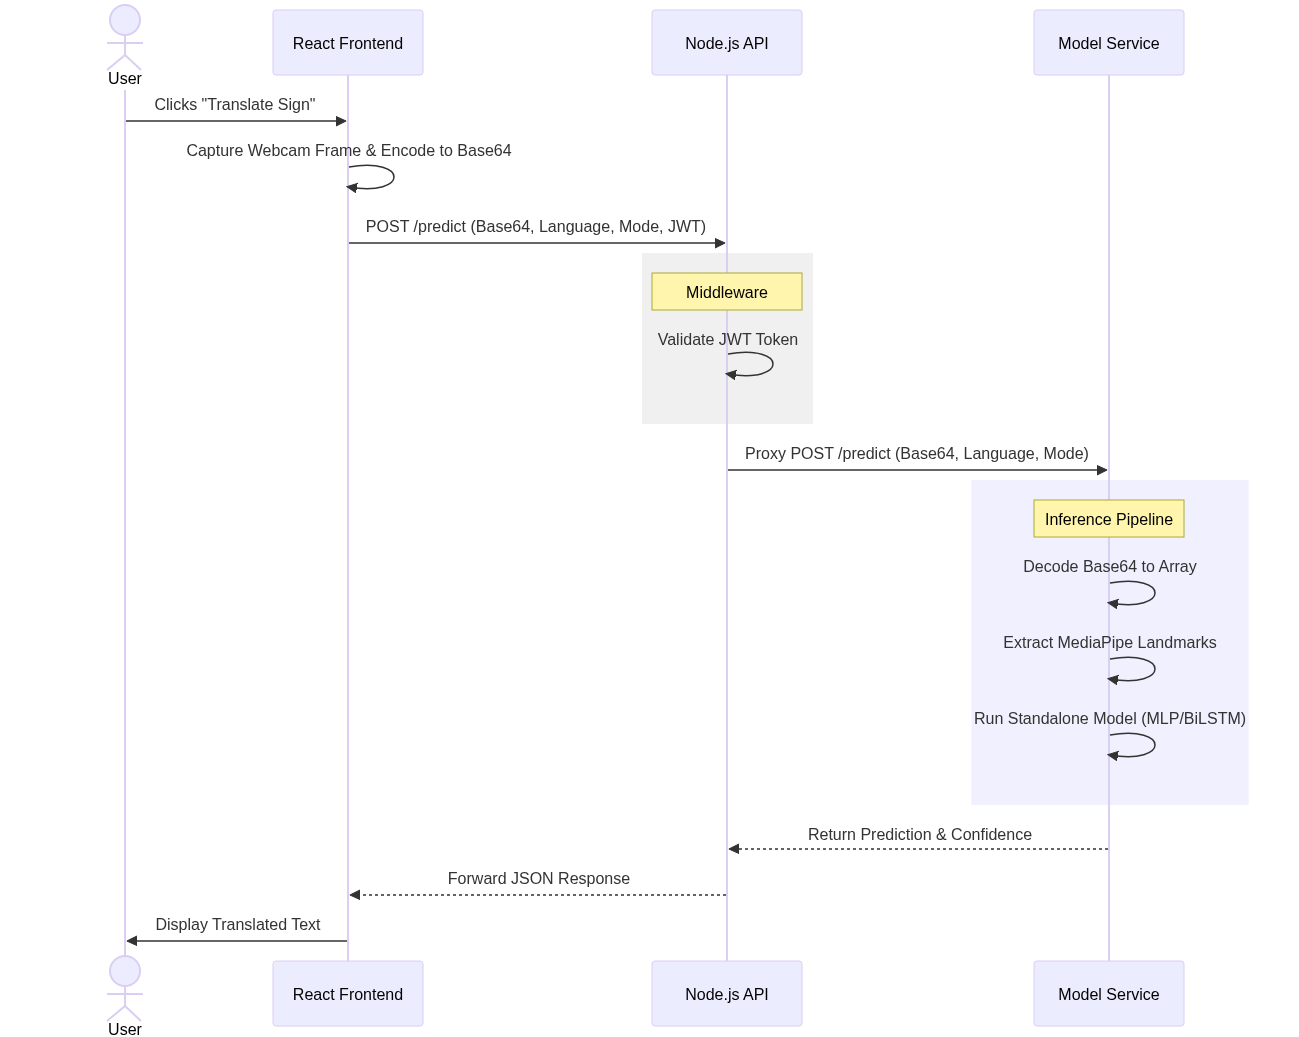
\includegraphics[width=0.925\textwidth]{images/fig_7-3_sequence_diagram.png}
\caption{Sequence diagram of the end-to-end translation request: React client $\rightarrow$ Node.js API (JWT validation) $\rightarrow$ FastAPI model service (MediaPipe landmark extraction, model inference) $\rightarrow$ JSON response relayed back to the client.}
\label{fig:ch7-sequence}
\end{figure}
\vspace{0.2cm}

\noindent\textbf{5.5.3\quad Model inference pipeline:}\par
\addcontentsline{toc}{subsection}{\numberline{5.5.3}Model inference pipeline:}
\vspace{0.2cm}

\noindent Upon receiving the payload, the FastAPI service interprets the request body's \texttt{language} (\texttt{en} | \texttt{ar}) and \texttt{mode} (\texttt{letters} | \texttt{words}) fields to instantiate the appropriate inference engine. In letter mode, incoming base64 imagery is routed to either \texttt{asl\_\allowbreak mlp\_\allowbreak inference.py} (English) or \texttt{arsl\_\allowbreak mlp\_\allowbreak inference.py} (Arabic). These modules perform real-time MediaPipe hand-landmark extraction and execute the corresponding MLP classifier (defined in Chapter~3 using 63-D/78-D features) to predict the highest-confidence character. Finally, the service packages the prediction into a JSON response, which is relayed through the Node.js API to the React client for injection into the user's input buffer or live-chat stream.\par\vspace{0.3cm}

\noindent\textbf{Word-mode integration status.} At the time of writing, the \texttt{english + words} combination is routed to the WLASL Inception I3D engine described in Section~5.6; the \texttt{arabic + words} combination is not yet wired to the deployed ArSL BiLSTM (Chapter~4, Model~4) inside this web application and currently falls back to a mock response, even though the underlying 225-D BiLSTM checkpoint is fully trained and evaluated offline at 99.62\,\% Top-1 (Chapters~6--7). Wiring the ArSL word model into \texttt{model-services} following the same \texttt{predict\_word(session\_id, image\_base64)} contract used for WLASL (Section~5.6) is listed as near-term integration work in Chapter~9.\par\vspace{0.3cm}

\noindent\textbf{5.6\quad ASL WORD MODEL INTEGRATION (WLASL / INCEPTION I3D)}\par
\addcontentsline{toc}{section}{\numberline{5.6}ASL WORD MODEL INTEGRATION (WLASL / INCEPTION I3D)}
\vspace{0.2cm}

\noindent The English word-recognition path required a different integration pattern from the landmark-based letter and ArSL-word models, because the ASL word model (Chapter~4, Model~3) is a PyTorch Inception I3D network consuming RGB clips rather than MediaPipe landmark vectors~\cite{carreira2017i3d,pytorch2024,li2020wlasl}. This work was carried out on a dedicated \texttt{add-wlasl-model} integration branch of the web application so that the stable \texttt{main} branch remained untouched while the RGB pipeline was wired in.\par\vspace{0.2cm}

\noindent\textbf{Migrated artifacts.} The FastAPI \texttt{model-services} package was extended with the I3D network definition, the pretrained 100-word checkpoint (\texttt{asl100.pt} / \texttt{asl\_word\_i3d.pt}), the WLASL gloss-to-index list, and \texttt{torch}/\texttt{torchvision} runtime dependencies (Chapter~4, Table~\ref{tab:ch4-artifacts}).\par\vspace{0.2cm}

\noindent\textbf{Stateful inference.} A dedicated \texttt{wlasl\_inference.py} module keeps one state dictionary per \texttt{session\_id} (a 32-frame deque, a 10-prediction voting window, last-commit timestamp, and last-committed word), so that multiple concurrent users are not confused with one another's clips. Each incoming frame is decoded, colour-converted, resized so its short side is 256\,px, centre-cropped to 224$\times$224, and mapped to $[-1,1]$ (the same preprocessing as Chapter~4, Figure~\ref{fig:ch4-asl-preprocess}) before being appended to that session's deque. 


\clearpage
\noindent\ Once 32 frames are buffered, the I3D network runs and its softmax output is pushed into a \textbf{10-prediction voting window}; a class is only \textbf{committed} once it is the majority vote in that window ($\geq$6/10), its confidence is $\geq$50\,\%, and at least 1.2\,s have passed since the last commit (mirroring the letter stabilisation decoder pattern from Chapter~3, Section~3.6) --- otherwise the endpoint reports a \texttt{buffering} status with the current best guess. On the Node.js side, the \texttt{predict} controller attaches the authenticated user's ID (\texttt{req.user.id}, or \texttt{"anonymous"} if the request is unauthenticated) as the \texttt{sessionId} forwarded to FastAPI, giving each logged-in user an isolated video buffer without the frontend having to manage session identifiers itself.\par\vspace{0.2cm}

\noindent\textbf{Routing.} The FastAPI \texttt{/predict} route was extended so that a request with \texttt{language="en"} and \texttt{mode="words"} is routed to the \texttt{wlasl\_inference} engine instead of a placeholder response, mirroring the same language/mode dispatch pattern already used for the letter MLPs (Section~5.5.3). This keeps a single request contract (\texttt{language}, \texttt{mode}, \texttt{imageBase64}) across all four models even though the ASL word path is architecturally the odd one out --- RGB frames rather than landmarks, and per-session server-side buffering rather than a single-frame forward pass.\par\vspace{0.3cm}

\noindent\textbf{5.7\quad NAVIGATION FLOW AND MAIN PAGES}\par
\addcontentsline{toc}{section}{\numberline{5.7}NAVIGATION FLOW AND MAIN PAGES}
\vspace{0.2cm}

\noindent The frontend uses \texttt{react-router-dom}~\cite{reactrouter2024} to govern navigation, with a flow that is linear and strictly gated by authentication status. Unauthenticated users land on the \textbf{Landing Page}, which presents an overview of the system and forms to register or log in. A custom \texttt{ProtectedRoute} higher-order component wraps the core application paths; if a user without a valid JWT attempts to reach the main dashboard, the router intercepts the navigation and redirects back to the Landing Page. Once authenticated, users are routed to the \textbf{App Home Page}, the central hub of the application, whose layout is split into two tabs: \textit{Chatting} (live translation and real-time messaging) and \textit{Educational} (sign-language visualisation and practice).\par\vspace{0.2cm}

\begin{figure}[H]
\centering
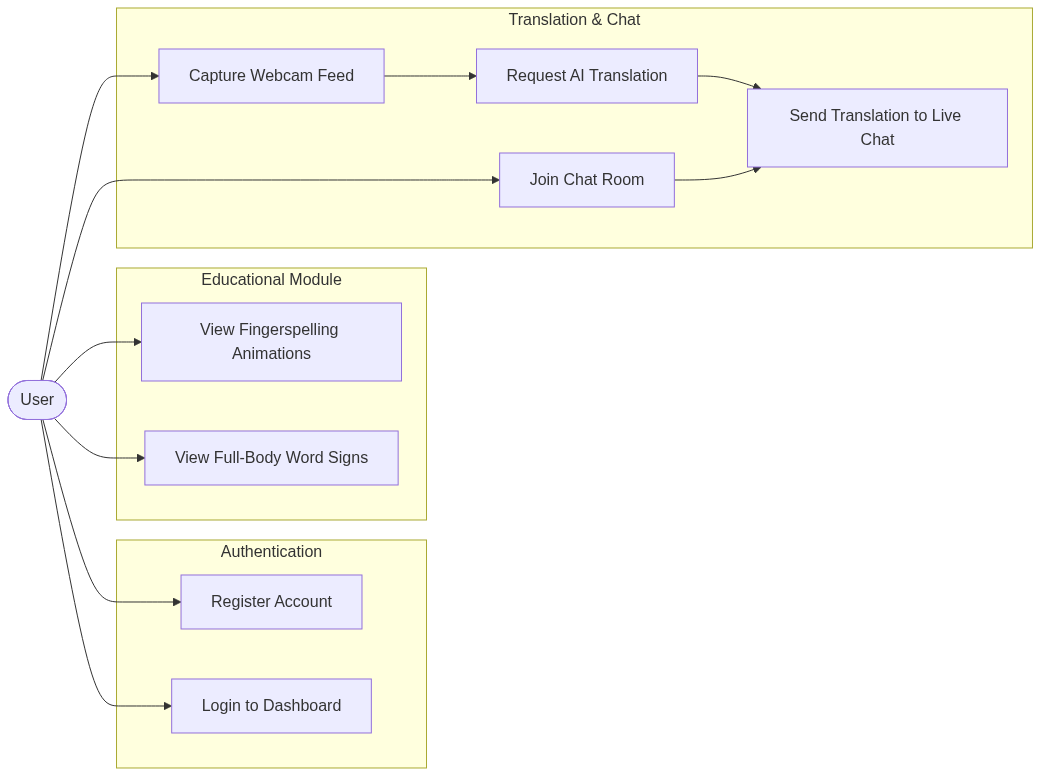
\includegraphics[width=1.00\textwidth]{images/fig_7-6_use_case.png}
\caption{Use case diagram: authentication (register/login), the Educational module (browse and watch word signs, fingerspell typed text, sign a typed sentence, practise signs with webcam feedback), and Translation \& Chat (capture webcam feed, request AI translation, join chat room, send translation to live chat).}
\label{fig:ch7-usecase}
\end{figure}
\vspace{0.3cm}

\noindent\textbf{Deployed web interface.} Figures~\ref{fig:ch7-login} and~\ref{fig:ch7-apphome} show the live Eshara web application. The \textbf{Landing Page} (Figure~\ref{fig:ch7-login}) carries the Eshara logo and tagline (\textit{``Sign language assistant with realtime chat''}), a Login/Register tab toggle, a dark-mode switch, and the credential form described in Section~5.3.2. The \textbf{App Home Page} (Figure~\ref{fig:ch7-apphome}) is reached only after authentication (Section~5.7) and shows the \textit{Chatting} tab active: language (\textit{English (ASL)}) and mode (\textit{Letters}/\textit{Words}) dropdowns, a camera-device selector (Section~5.2.4), the mirrored webcam panel with \textbf{Start Camera}/\textbf{End Camera}/\textbf{Translate Sign} controls and a live status line (\textit{``Camera is off''}), and the \textbf{Live Chat} panel on the right with a chat-partner selector, message history, and a text/translation input bar --- the concrete realisation of the Socket.IO messaging described in Section~5.3.3.\par\vspace{0.2cm}

\begin{figure}[H]
\centering
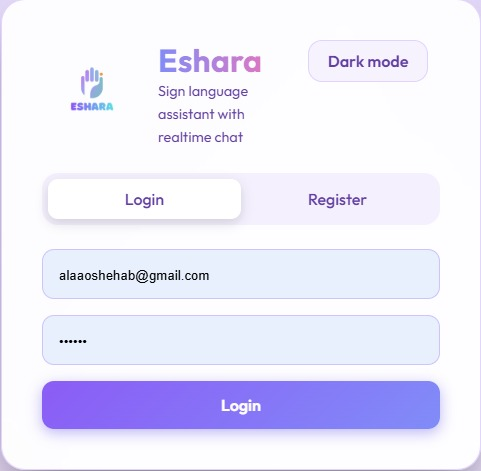
\includegraphics[width=0.54\textwidth]{images/fig_7-8_login_screen.png}
\caption{Eshara Landing Page: logo, tagline, Login/Register toggle, dark-mode switch, and credential form.}
\label{fig:ch7-login}
\end{figure}
\vspace{0.2cm}

\begin{figure}[H]
\centering
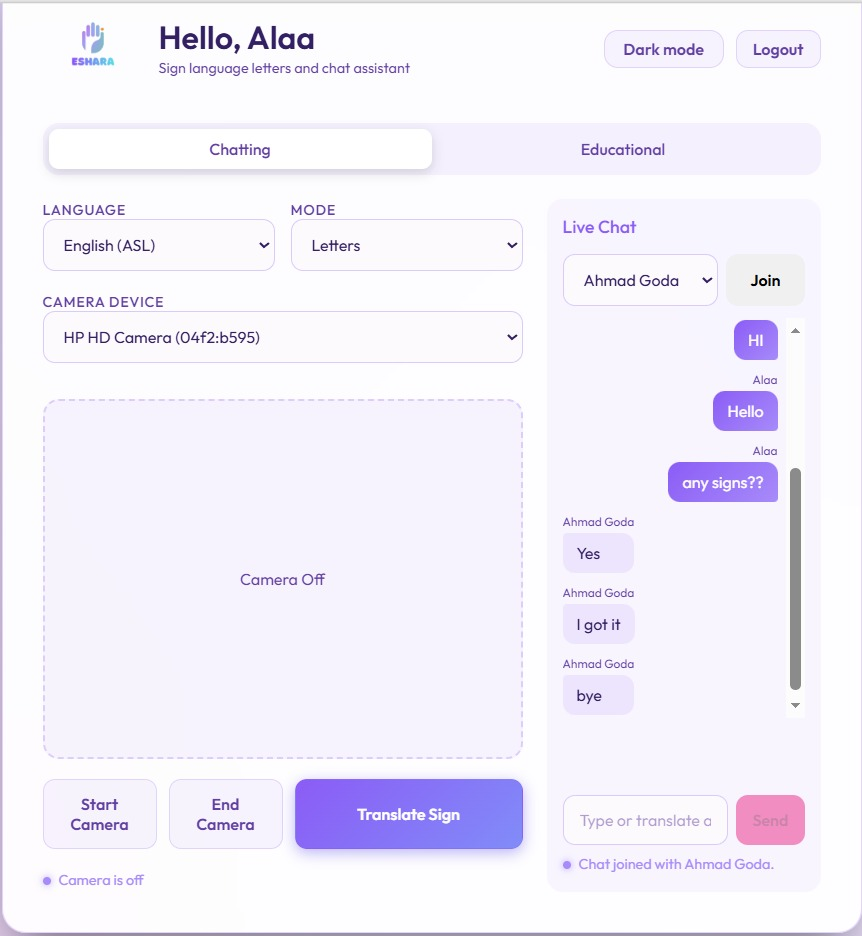
\includegraphics[width=0.54\textwidth]{images/fig_7-9_chat_translation_screen.png}
\caption{Eshara App Home Page (Chatting tab): language/mode/camera-device selectors, webcam capture panel with Start/End Camera and Translate Sign controls, and the Live Chat panel with an active Socket.IO room.}
\label{fig:ch7-apphome}
\end{figure}
\vspace{0.2cm}

\noindent\textbf{5.8\quad FEATURES, FUNCTIONALITY, AND UX DESIGN}\par
\addcontentsline{toc}{section}{\numberline{5.8}FEATURES, FUNCTIONALITY, AND UX DESIGN}
\vspace{0.1cm}

\noindent\textbf{Live chat and AI translation.} The flagship feature merges standard text messaging with AI-driven translation: the user selects a target language (ASL/ArSL) and scope (letters/words); the mirrored webcam feed lets the user see themselves naturally while signing; and, once a translation is produced, the predicted output is appended to the chat buffer and can be emitted to a live Socket.IO room, enabling cross-user communication carried out entirely in sign language.\par\vspace{0.1cm}

\noindent\textbf{Educational tools.} The Educational tab hosts three bilingual (ASL/ArSL) learning tools --- a categorised \textit{Sign Viewer} with integrated fingerspelling, a free-text \textit{Sentence Builder}, and a webcam \textit{Practice} mode --- built on motion-capture skeleton playback with server-side animation stitching; the module is documented in full in Section~5.14 (Part~B).\par\vspace{0.1cm}

\noindent\textbf{Responsive design and feedback.} CSS media queries and a flexible \texttt{display: grid} layout let the interface adapt fluidly from desktop monitors to small mobile viewports, stacking side-by-side panels (camera feed and chat window) vertically on constrained screens~\cite{wcag22}. Every interaction gives immediate visual feedback: translation requests trigger a temporary \textit{``Translating\ldots''} state, and socket connections display \textit{``Connected''} or \textit{``Error''} banners; modern micro-animations are used sparingly to keep the interface responsive without clutter.\par\vspace{0.3cm}

\noindent\textbf{5.9\quad SECURITY CONSIDERATIONS}\par
\addcontentsline{toc}{section}{\numberline{5.9}SECURITY CONSIDERATIONS}
\vspace{0.1cm}

\noindent\textbf{Authentication and cryptography.} User passwords are never stored in plaintext; they are hashed with \texttt{bcryptjs} using a high salt round before insertion into the database~\cite{bcrypt2024}. Sessions are managed statelessly via JWTs, so authentication tokens are cryptographically signed and tamper-evident~\cite{rfc7519}.\par\vspace{0.1cm}

\noindent\textbf{Encapsulated ML tier.} The FastAPI model service is explicitly hidden behind the Node.js application server; because the ML service ports are never exposed to the public internet, the attack surface is significantly reduced and every translation request must pass through the Node.js authentication middleware before reaching the inference engine.\par\vspace{0.1cm}

\noindent\textbf{CORS and input validation.} Cross-Origin Resource Sharing is strictly configured on the backend to prevent unauthorised domains from calling the APIs, and input payloads --- particularly login credentials and large base64 image strings --- are validated before processing to mitigate injection attacks and buffer-overload abuse. Transmitting landmark vectors rather than raw video for the letter and ArSL-word paths (Chapter~2, Chapter~7 Section~7.6) further reduces the amount of biometric image data that ever leaves the client for two of the four models; the ASL word path, which must transmit RGB frames for the I3D network, does not carry this benefit and is discussed as a residual privacy trade-off in Chapter~7.\par

\clearpage
\noindent\textbf{5.10\quad DEPLOYMENT}\par
\addcontentsline{toc}{section}{\numberline{5.10}DEPLOYMENT}
\vspace{0.2cm}

\noindent Graduation deployment is \textbf{web-only} across three independently hostable tiers: the React SPA is served as a static build over HTTPS; the Node.js + Express application server runs as a long-lived process with its SQLite database file on a persistent volume and the Socket.IO server attached to the same HTTP instance; and the FastAPI service runs in an isolated ML inference environment with the four model checkpoints loaded from disk. No app-store packaging, React Native wrapper, or on-device TensorFlow Lite/PyTorch Mobile export is part of the graduation deliverable.\par\vspace{0.2cm}

\begin{figure}[H]
\centering
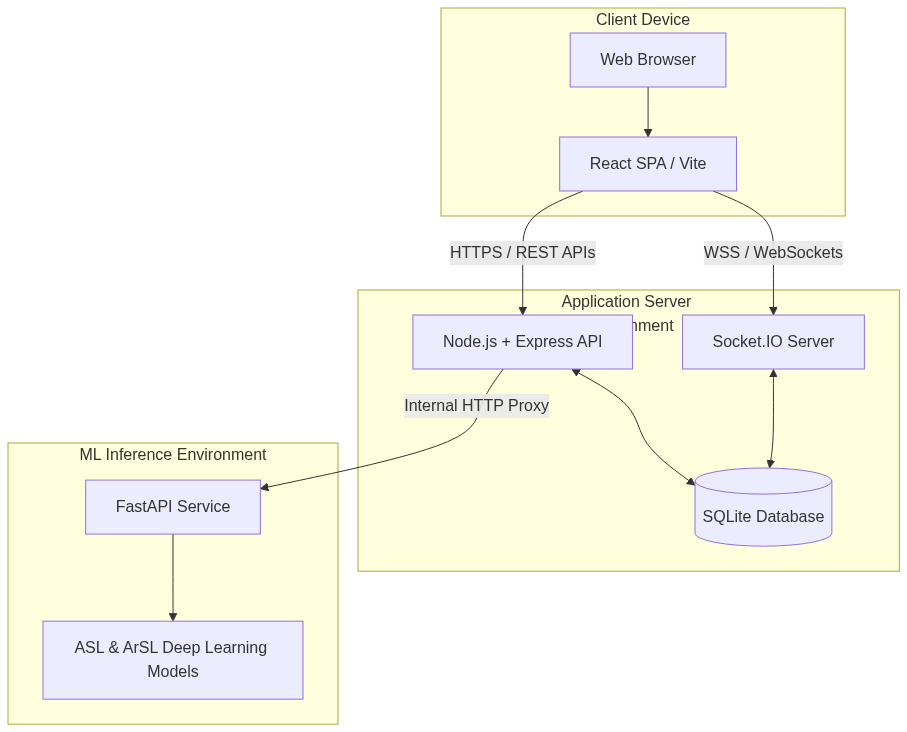
\includegraphics[width=1.10\textwidth]{images/fig_7-7_deployment_diagram.png}
\caption{Deployment diagram: client device (browser, React SPA) communicating over HTTPS/REST and WSS/WebSockets with the application server (Node.js + Express, Socket.IO, SQLite), which forwards inference requests over an internal HTTP proxy to the isolated ML inference environment (FastAPI service, ASL/ArSL deep-learning models).}
\label{fig:ch7-deployment}
\end{figure}
\vspace{0.3cm}

\noindent\textbf{5.11\quad ERROR HANDLING AND TESTING}\par
\addcontentsline{toc}{section}{\numberline{5.11}ERROR HANDLING AND TESTING}
\vspace{0.2cm}

\noindent\textbf{5.11.1\quad Graceful degradation:}\par
\addcontentsline{toc}{subsection}{\numberline{5.11.1}Graceful degradation:}
\vspace{0.2cm}

\noindent On the client, global Axios interceptors catch \texttt{401 Unauthorized} responses to purge invalid sessions and redirect the user, and browser APIs such as \texttt{navigator.mediaDevices} are wrapped in \texttt{try/catch} blocks so that a denied or missing webcam falls back to human-readable troubleshooting instructions rather than a silent failure. On the server, Express controllers wrap external calls in \texttt{try/catch}; if the FastAPI service is offline, the Node.js proxy catches the failed fetch and returns a structured \texttt{503 Service Unavailable} response instead of allowing the primary server process to crash.\par\vspace{0.2cm}

\noindent\textbf{5.11.2\quad Testing methodology:}\par
\addcontentsline{toc}{subsection}{\numberline{5.11.2}Testing methodology:}
\vspace{0.2cm}

\noindent The application underwent manual interface and integration testing covering real-time Socket.IO chat latency, responsive layout reflow on constrained mobile viewports, and cross-browser webcam access. Independently of the web integration, each backend ML model was evaluated against its own standardised dataset split before integration (Chapter~6); integration testing then confirmed that frontend JPEG base64 compression does not introduce artifacts that materially degrade active web inference paths during live webcam use.\par\vspace{0.3cm}

\noindent\textbf{5.12\quad REAL-TIME WEB PERFORMANCE}\par
\addcontentsline{toc}{section}{\numberline{5.12}REAL-TIME WEB PERFORMANCE}
\vspace{0.2cm}

\noindent Chapter~1 hypothesised end-to-end latency $\leq 200$\,ms from frame capture to displayed text on a standard laptop. As reported in the following table, \textbf{pilot measurements} on graduation development hardware (Windows 11 laptop, Chrome, 720p webcam, localhost stack) use 100 samples per row, timed with \texttt{performance.now()} in the browser and server wall-clock around \texttt{model.predict}; the full measurement protocol is documented in the project evaluation notes.\par\vspace{0.2cm}

\begin{table}[H]
\centering
\caption{Real-time web performance (pilot measurements, graduation dev hardware).}
\label{tab:ch7-latency}
\small
\begin{tabular}{|l|l|c|c|}
\hline
\multicolumn{1}{|c|}{\textbf{Component}} & \multicolumn{1}{|c|}{\textbf{How measured}} & \multicolumn{1}{|c|}{\textbf{p50}} & \multicolumn{1}{|c|}{\textbf{p95}}\\
\hline
MediaPipe (FastAPI, server-side) & 100 frames, server wall-clock around landmark extraction & 34 ms ($\sim$29 FPS) & 48 ms \\
\hline
Server inference (letter MLP) & FastAPI timing around predict & 4 ms & 7 ms \\
\hline
Server inference (ArSL word BiLSTM) & 48-frame batch (offline-validated path) & 24 ms & 38 ms \\
\hline
Server inference (ASL word I3D) & 32-frame RGB batch (CUDA) & 92 ms & 128 ms \\
\hline
HTTP \texttt{/predict} round-trip (letter) & Client POST $\rightarrow$ Node proxy $\rightarrow$ JSON response & 11 ms & 19 ms \\
\hline
\textbf{E2E letter} & Frame $\rightarrow$ UI label update & \textbf{51 ms} & 74 ms \\
\hline
\textbf{E2E ArSL word (offline-validated)} & FastAPI inference after 48-frame buffer & 41 ms & 68 ms \\
\hline
\textbf{E2E ASL word} & Inference after 32-frame buffer & 108 ms & 145 ms \\
\hline
\end{tabular}
\end{table}
\vspace{0.3cm}

\noindent Letter mode satisfies the $\leq 200$\,ms hypothesis (p50\,=\,51\,ms). Word modes incur an additional \textbf{buffer-fill} delay ($\sim$1.0--1.6\,s at 30\,FPS for 32--48 frames) before the first inference; per-commit server latency remains below 150\,ms. Server-side MediaPipe extraction dominates the letter-path compute budget before the MLP forward pass; letter MLP inference remains under 5\,ms on CPU as expected from Chapter~3 architecture size. ArSL word rows in Table~\ref{tab:ch7-latency} reflect the offline-validated FastAPI path documented in Section~5.5.3, not the current mock web response for \texttt{arabic + words}.\par\vspace{0.3cm}

\noindent\textbf{5.13\quad INFORMAL USABILITY PILOT}\par
\addcontentsline{toc}{section}{\numberline{5.13}INFORMAL USABILITY PILOT}
\vspace{0.2cm}

\noindent A formal deaf-community study with System Usability Scale (SUS) scoring was out of graduation scope (Chapter~6, Section~6.6). An \textbf{informal pilot} ($N{=}3$ student testers, 15-minute sessions each) exercised all four modes in the React UI. The following table records structured observations; a full SUS study with 10+ participants is recommended in Chapter~9~\cite{wcag22}.\par\vspace{0.2cm}

\begin{table}[H]
\centering
\caption{Informal usability pilot observations ($N{=}3$, React web UI).}
\label{tab:ch7-usability}
\small
\begin{tabular}{|l|c|l|}
\hline
\multicolumn{1}{|c|}{\textbf{Criterion}} & \multicolumn{1}{|c|}{\textbf{Rating}} & \multicolumn{1}{|c|}{\textbf{Notes}}\\
\hline
Camera setup ($<$1 min) & Good & Standard browser permission flow \\
\hline
Letter mode clarity & Good & Stabilisation reduces flicker; J/Z motion weak \\
\hline
ArSL word mode clarity & Good & 48-frame buffer requires full sign duration \\
\hline
ASL word mode clarity & Fair & Framing sensitivity; 32-frame window \\
\hline
RTL Arabic display & Good & Sentence builder readable \\
\hline
Mode switching (letter/word) & Fair & Manual toggle; no auto-detection \\
\hline
Overall assistive potential & Good & Suitable for practice, not certified interpretation \\
\hline
\end{tabular}
\end{table}
\vspace{0.2cm}

\clearpage
\begin{center}{\large \textbf{PART B --- EDUCATION MODULE}}\end{center}
\vspace{0.1cm}

\noindent\textbf{5.14\quad EDUCATION MODULE: BILINGUAL SIGN-LANGUAGE LEARNING}\par
\addcontentsline{toc}{section}{\numberline{5.14}EDUCATION MODULE: BILINGUAL SIGN-LANGUAGE LEARNING}
\vspace{0.2cm}

\noindent This section documents the Education tab at the same technical depth as Part~A's Translation \& Chat features. The module was rebuilt during the final development cycle around \textbf{motion-capture skeleton playback}: signs are no longer drawn as hand-authored stick-figure keyframes but replayed from pose recordings of real signers, and the module grew from two ASL practice panels into three bilingual learning tools. In both American Sign Language and Arabic Sign Language the tab offers a \textbf{Sign Viewer} (browse a categorised vocabulary and watch each sign, or fingerspell any typed word), a \textbf{Sentence Builder} (type a free-form sentence and watch it signed end-to-end), and a \textbf{Practice} mode (perform a prompted sign into the webcam and get instant feedback from the same recognition models that power the Chatting tab). Unlike the earlier canvas-only iteration, the Education tab is now a client--server feature: animation assembly runs in the FastAPI model-services tier, which stitches multiple sign clips into one smooth animation and streams it to the browser.\par\vspace{0.3cm}

\noindent\textbf{5.14.1\quad Overview and layout:}\par
\addcontentsline{toc}{subsection}{\numberline{5.14.1}Overview and layout:}
\vspace{0.2cm}

\noindent The Education tab is one of the two primary tabs on the App Home Page alongside Chatting (Section~5.7). A header sub-navigation carries a language toggle --- \textit{ASL~$\cdot$~English} / \textit{ArSL~$\cdot$~\arTxt{العربية}} --- and a tool switch between the Sign Viewer, the Sentence Builder, and Practice mode. Switching languages remounts the tool components with a React \texttt{key=\{lang\}}, so selection, playback, and camera state reset naturally without manual synchronisation logic. Each component receives its language-specific configuration (word list, categories, alphabet, text direction, placeholder copy) from a single \texttt{LANG\_CONFIG} lookup, so the English and Arabic experiences share one code path.\par\vspace{0.2cm}

\begin{figure}[H]
\centering
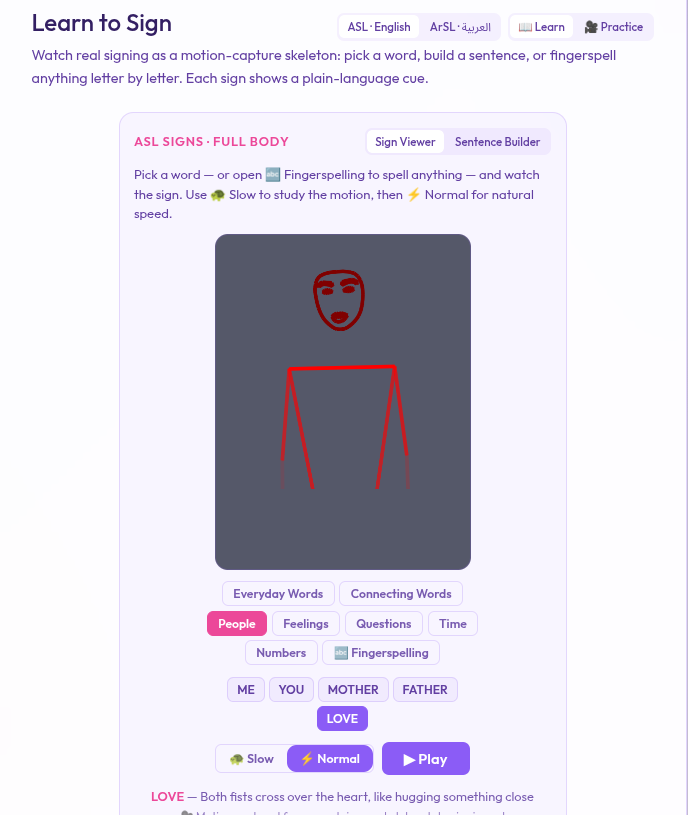
\includegraphics[width=0.62\textwidth]{images/fig_5-10_education.png}
\caption{Eshara Education tab (Sign Viewer, ASL): motion-capture skeleton playback with categorised vocabulary and playback-speed controls.}
\label{fig:ch5-edu-viewer}
\end{figure}
\vspace{0.2cm}

\noindent\textbf{5.14.2\quad Motivation: from hand-authored keyframes to motion capture:}\par
\addcontentsline{toc}{subsection}{\numberline{5.14.2}Motivation: from hand-authored keyframes to motion capture:}
\vspace{0.2cm}

\noindent An earlier iteration of this module rendered signs with a bespoke Canvas2D stick figure: every sign was a manually authored sequence of wrist keyframes and procedurally constructed handshapes, resolved through a two-joint inverse-kinematics solver. That engine was fast and dependency-free, but it could not scale in either quantity or quality. Each new sign required careful manual authoring and a geometric verification pass (hands visually merging, contact points floating off the head), the vocabulary plateaued at fifteen words, and even a correct keyframe animation reads as a symbolic illustration rather than a human performing the sign --- a material pedagogical weakness for a learning tool.\par\vspace{0.2cm}

\noindent The module was therefore rebuilt on \textbf{skeleton recordings of real signers}. Every sign is a \texttt{.pose} file --- the standard binary format of the \texttt{pose-format} library~\cite{poseformat} --- containing per-frame MediaPipe Holistic landmarks (body, face, and both hands) extracted from video of a human signer~\cite{zhang2020mediapipe}, replayed in the browser by the \texttt{<pose-viewer>} web component from the sign-language-processing project (the same renderer used by the open-source sign.mt translation platform~\cite{signmt2023}). This reversal of the earlier decision to avoid \texttt{<pose-viewer>} was deliberate and evidence-based: the lag that originally motivated the Canvas2D rewrite was caused not by the renderer itself but by playing many small clips back-to-back with client-side fetches between them. The rebuilt module fixes the root cause with server-side animation stitching (Section~5.14.4) --- one continuous animation per Play press --- while gaining human motion data, per-finger articulation, and a content pipeline that can grow the vocabulary without manual animation work. The legacy canvas stickman remains only as a fallback renderer for the few English words that have hand-authored keyframes but no \texttt{.pose} file.\par\vspace{0.3cm}

\noindent\textbf{5.14.3\quad Content pipeline: dictionary signs from sign.mt:}\par
\addcontentsline{toc}{subsection}{\numberline{5.14.3}Content pipeline: dictionary signs from sign.mt:}
\vspace{0.2cm}

\noindent Sign content is fetched offline from sign.mt's public dictionary API (\texttt{model-services/fetch\_signmt\_pose.py}), which translates a spoken-language word into a signed-language pose clip drawn from a curated dictionary: American Sign Language (\texttt{ase}) for English and Jordanian Sign Language (\texttt{jos}) for Arabic --- the only openly available Arabic-lookup sign dictionary~\cite{signmt2023}. The deployed vocabulary counts 44 English words plus the 26-letter manual alphabet, and 42 verified Arabic word signs plus the 28-letter Arabic alphabet; every clip is attributed on-page (\textit{``Motion captured from a real signer''}). Critically, the API silently returns a \textbf{fingerspelled} letter sequence, with HTTP~200, for any word its dictionary does not contain --- so a successful fetch does not prove the dictionary has the sign. The verification methodology built to defeat this failure mode is documented in Section~5.14.8.\par\vspace{0.2cm}

\noindent One rendering subtlety is worth recording. The \texttt{pose-viewer} custom element upgrades lazily, and a false JSX boolean attribute is removed from the DOM entirely --- so \texttt{autoplay=\{false\}} never reaches the component, whose internal default is \texttt{true}. Each component therefore sets \texttt{el.autoplay = false} imperatively in a mount effect, and drives playback through the component's \texttt{play()}/\texttt{pause()} methods and its \texttt{loadeddata\$}~/~\texttt{ended\$} events.\par\vspace{0.3cm}

\noindent\textbf{5.14.4\quad Server-side animation stitching (\texttt{pose\_concat.py}):}\par
\addcontentsline{toc}{subsection}{\numberline{5.14.4}Server-side animation stitching (\texttt{pose\_concat.py}):}
\vspace{0.2cm}

\noindent Playing letter or word clips back-to-back on the client produced the original module's characteristic lag: between every two clips the skeleton snapped from one pose to another, with a network fetch in between. All multi-sign playback was therefore moved server-side. The FastAPI tier stitches the requested signs into \textbf{one} \texttt{.pose} file using \texttt{spoken-to-signed} --- sign.mt's own concatenation package~\cite{spokentosigned} --- and streams the finished animation to the client:
\begin{enumerate}
\item Each clip is reduced (redundant landmarks dropped), normalised, and trimmed at its natural signing boundaries (a wrist-above-elbow heuristic finds where signing actually starts and ends).
\item Adjacent clips are cut at their best \textbf{connection point} --- the frame pair where the two skeletons are geometrically closest --- so one sign flows into the next.
\item A short zero-confidence gap (0.2\,s) is inserted at every boundary and filled by interpolation; the whole sequence is then smoothed with a Savitzky--Golay filter, wrist positions are corrected, and the result is size-normalised.
\end{enumerate}
\vspace{0.1cm}

\noindent Three language-parameterised endpoint families expose this pipeline:
\begin{itemize}
\item \texttt{/api/pose-seq} (\texttt{mode=words}) --- stitches a list of named signs with natural trimmed motion; used when the Sign Viewer plays a word.
\item \texttt{/api/pose-seq} (\texttt{mode=spell}) --- fingerspelling mode. Letter clips are inconsistent upstream (some are 3-frame stills, some full 25/30\,fps clips), and connection-point cutting can shrink a letter to a few unreadable frames --- so spell mode instead slices each letter to its central held handshape and freezes it for 0.35\,s, producing a uniform, readable spelling rhythm.
\item \texttt{/api/pose-text} --- free-text mode for the Sentence Builder (Section~5.14.6).
\end{itemize}
\vspace{0.1cm}

\noindent Every stitching endpoint has a \texttt{/meta} twin returning per-segment durations on the final timeline; because the animation itself is a single opaque file, synchronised UI feedback (highlighting the word chip or letter currently playing) is driven entirely by this metadata with plain client-side timers. Results are memoised server-side (\texttt{functools.lru\_cache}) so a repeated Play press is a cache hit, and \texttt{Content-Disposition} headers use RFC~5987 encoding because Arabic filenames cannot be represented in latin-1 HTTP headers. Sentence input is bounded (12 tokens, 80 stitched segments) so a pathological request cannot exhaust the service.\par\vspace{0.3cm}

\noindent\textbf{5.14.5\quad Sign Viewer:}\par
\addcontentsline{toc}{subsection}{\numberline{5.14.5}Sign Viewer:}
\vspace{0.2cm}

\noindent The Sign Viewer presents the language's vocabulary as category tabs (\textit{Everyday Words}, \textit{People}, \textit{Feelings}, \ldots; \arTxt{كلمات يومية}, \arTxt{الناس}, \arTxt{مشاعر وصفات}, \ldots) with one button per word. Selecting a word previews its first frame; Play streams the sign at \textit{Slow} (0.5$\times$) or \textit{Normal} (1$\times$, the default) speed, and each word is captioned with its meaning --- for Arabic, an English gloss, since the app's UI language is English. A final tab, \textit{Fingerspelling}, replaces the word grid with a letter reference grid (A--Z for ASL; the 28 Arabic base letters for ArSL) whose buttons play each letter's held handshape, plus a free spelling input: any typed word is filtered to spellable letters and played as one server-stitched spell-mode sequence, with the on-screen grid highlighting each letter in sync via the \texttt{/meta} timing data. If the configured default word is ever pruned from the vocabulary, the component falls back to the first available word rather than rendering an empty viewer.\par\vspace{0.2cm}

\begin{figure}[H]
\centering
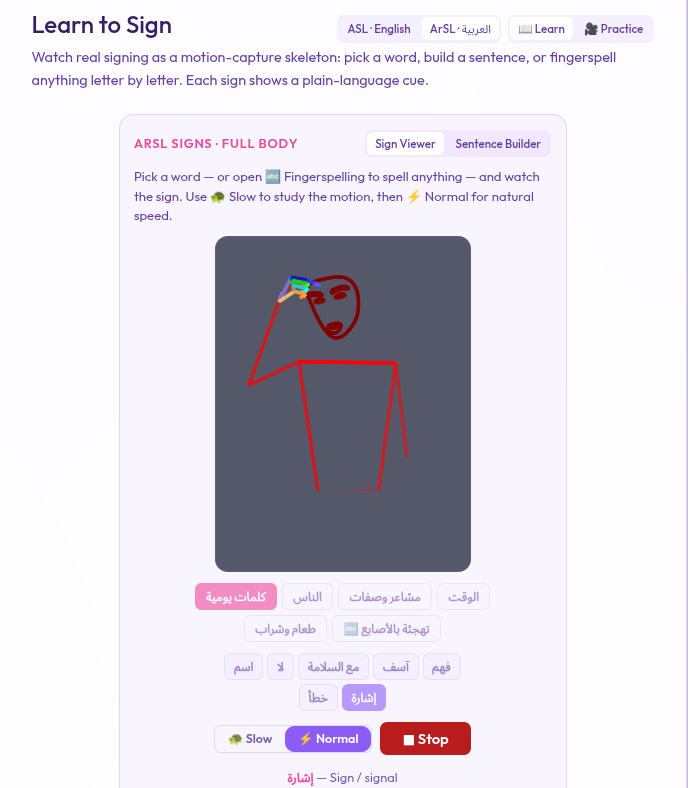
\includegraphics[width=0.62\textwidth]{images/fig_5-11_education.png}
\caption{Sign Viewer (ArSL): Jordanian Sign Language skeleton playback with right-to-left category and word controls.}
\label{fig:ch5-edu-arsl}
\end{figure}

\begin{figure}[H]
\centering
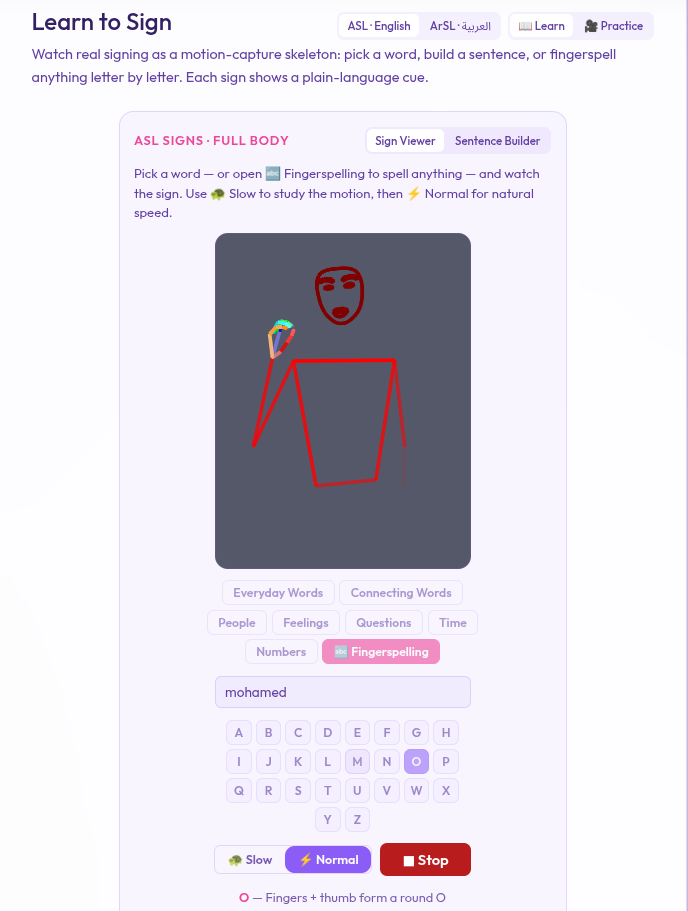
\includegraphics[width=0.62\textwidth]{images/fig_5-12_education.png}
\caption{Fingerspelling: a typed word plays as one server-stitched sequence while the current letter is highlighted from timing metadata.}
\label{fig:ch5-edu-spell}
\end{figure}
\vspace{0.2cm}

\noindent\textbf{5.14.6\quad Sentence Builder --- free-text signing:}\par
\addcontentsline{toc}{subsection}{\numberline{5.14.6}Sentence Builder --- free-text signing:}
\vspace{0.2cm}

\noindent The Sentence Builder follows sign.mt's interaction model: the user types any sentence; words found in the sign dictionary are signed, and unknown words are fingerspelled letter by letter~\cite{signmt2023}. The server's plan builder (\texttt{pose\_concat.build\_text\_sequence}) implements this as follows:
\begin{enumerate}
\item The text is tokenised (lowercased; Arabic diacritics stripped; digits 1--5 and Arabic-Indic \arTxt{١}--\arTxt{٥} mapped to their number words).
\item Tokens are matched greedily against the dictionary, longest phrase first (3-gram, then 2-gram, then single word) --- multi-word entries such as \textit{``thank you''} or \arTxt{مع السلامة} exist as \textbf{one} pose file and must not be split into unknown singles and spelled.
\item Lookups are orthography-tolerant (Section~5.14.7): both the query and the stored filenames are folded before comparison.
\item Any token still unmatched is decomposed into its letters and fingerspelled inline, using the same held-peak treatment as the Fingerspelling tab.
\item The full plan is stitched into one smooth animation and returned with per-token and per-letter timing metadata.
\end{enumerate}
\vspace{0.1cm}

\noindent The frontend mirrors the same greedy matching client-side to render a live \textbf{chip preview} as the user types: solid chips are words that will be signed from the dictionary; dashed chips carrying a fingerspelling marker will be spelled. This honesty matters --- a learner must never mistake a spelled word for the word's actual sign. During playback the chips and, for spelled tokens, the individual letters light up in sync with the animation.\par\vspace{0.2cm}

\begin{figure}[H]
\centering
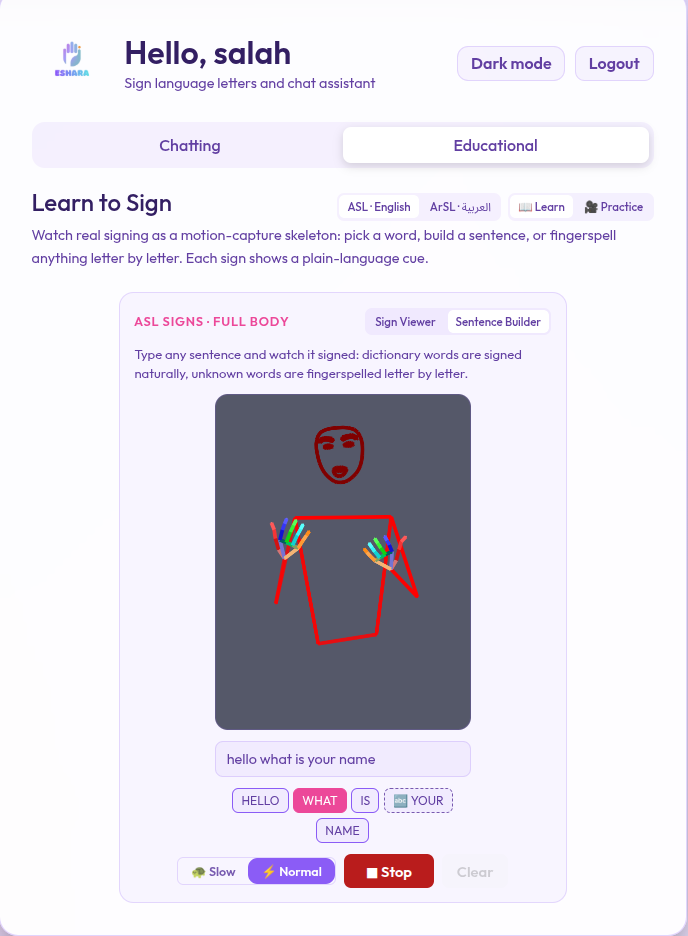
\includegraphics[width=0.62\textwidth]{images/fig_5-13_education.png}
\caption{Sentence Builder: dictionary words render as solid chips and are signed; unknown words render as dashed chips and are fingerspelled, with live highlighting driven by timing metadata.}
\label{fig:ch5-edu-sentence}
\end{figure}
\vspace{0.2cm}

\noindent\textbf{5.14.7\quad Arabic support (ArSL):}\par
\addcontentsline{toc}{subsection}{\numberline{5.14.7}Arabic support (ArSL):}
\vspace{0.2cm}

\noindent Every pose endpoint takes \texttt{lang=en|ar} and resolves content from a per-language directory. The tools are fully parameterised for Arabic: right-to-left text direction on inputs and labels, Arabic-Indic digit handling, and Arabic category labels. Two Arabic-specific engineering problems are worth recording:
\begin{itemize}
\item \textbf{Orthographic variance.} Arabic words are commonly typed without hamza/madda marks (\arTxt{ام} for \arTxt{أم}, \arTxt{اسف} for \arTxt{آسف}), yet the sign dictionary keys many entries under proper orthography --- and vice versa. A single folding table (\arTxt{أ}\,\arTxt{إ}\,\arTxt{آ}\,$\rightarrow$\,\arTxt{ا}; \arTxt{ى}\,\arTxt{ئ}\,$\rightarrow$\,\arTxt{ي}; \arTxt{ؤ}\,$\rightarrow$\,\arTxt{و}; \arTxt{ة}\,$\rightarrow$\,\arTxt{ه}; \arTxt{ء} dropped) is applied to \textbf{both} sides of every lookup: the server resolves queries through a folded-name index, and the client mirrors the same fold for chip previews and practice-answer matching. Files keep their proper spellings; users may type either form.
\item \textbf{Fingerspelling alphabet.} ArSL fingerspelling uses the 28 base letters; variant forms fold onto the letters that have clips (e.g.\ \arTxt{ة} spells as \arTxt{ه}), and diacritics are stripped before spelling.
\end{itemize}
\vspace{0.1cm}

\noindent Two linguistic caveats are documented for the record. First, the Arabic sign content is Jordanian Sign Language (\texttt{jos}) --- the only openly available Arabic sign dictionary --- while the ArSL recognition models were trained on KArSL (Saudi) data~\cite{sidig2021karsl}; regional sign variants differ, so the viewer and the recogniser are not guaranteed to agree on every word. Second, sentence signing follows the typed word order (a transliteration); it does not reorder into natural sign-language grammar. Both are acceptable for a learning aid but are stated honestly in the interface and in this thesis.\par\vspace{0.3cm}

\noindent\textbf{5.14.8\quad Content verification --- defeating the silent fallback:}\par
\addcontentsline{toc}{subsection}{\numberline{5.14.8}Content verification --- defeating the silent fallback:}
\vspace{0.2cm}

\noindent The hardest data-quality problem in the module was the dictionary API's silent fallback: for an out-of-vocabulary word it returns a fingerspelled letter sequence that is indistinguishable, at the protocol level, from a real sign. Publishing such a clip as a word sign would teach learners something actively wrong, and visual review alone proved unreliable --- a reviewer who does not know Jordanian Sign Language cannot always tell an unfamiliar sign from a spelled sequence. An automated classifier was therefore built:
\begin{enumerate}
\item For a candidate word, fetch the word itself \textbf{and} the doubled word (the word concatenated with itself). The doubled form is guaranteed to be out-of-vocabulary, so its returned animation is, by construction, the cloud's own spelling of the word, processed by the identical pipeline.
\item Reduce both animations to per-frame \textbf{handshape descriptors}: the 21 right-hand landmarks, wrist-relative and scale-normalised, so global position and size differences cancel.
\item Compare with start-anchored \textbf{dynamic time warping} (DTW), which absorbs the timing differences the stitching pipeline introduces. If the word's animation matches the spelling's prefix, it \textbf{is} the spelling fallback. Scores separate cleanly: spelled $<0.9$, real $\geq 2.9$.
\end{enumerate}
\vspace{0.1cm}

\noindent Every accepted clip was additionally reviewed frame-by-frame as a rendered filmstrip. A sweep of roughly 170 candidate Arabic words produced two further discoveries. First, the dictionary keys many entries under proper orthography only --- \arTxt{أم} is a real sign while \arTxt{ام} comes back spelled --- which directly motivated the fold-everywhere lookup of Section~5.14.7. Second, words containing \arTxt{ة} crash the API with HTTP~500 when out-of-vocabulary (its spelling lexicon lacks that letter), which turns the status code into a truth oracle for that word class. The final Arabic vocabulary --- verified word signs only --- is exactly the set that passed all checks; everything else fingerspells honestly with the dashed-chip treatment.\par\vspace{0.3cm}

\noindent\textbf{5.14.9\quad Practice mode --- learn by doing:}\par
\addcontentsline{toc}{subsection}{\numberline{5.14.9}Practice mode --- learn by doing:}
\vspace{0.2cm}

\noindent Practice mode closes the learning loop: after watching a sign, the user performs it. The panel reuses the exact camera-and-predict pipeline that powers the live Chatting tab --- extracted into a shared \texttt{useCamera} hook --- with its own camera instance so the two tabs never interfere:
\begin{itemize}
\item \textbf{Letter practice:} the panel prompts a random letter; the user poses it and a single webcam frame is sent to \texttt{POST /predict} (\texttt{mode=letters}). The models return exactly the comparison target --- an uppercase English letter or a real Arabic glyph --- so matching is a normalised string comparison.
\item \textbf{Word practice:} the panel prompts a word, runs a 3-2-1 countdown (cued performance needs reaction time), records a 3.2-second clip, and sends it to \texttt{POST /predict} (\texttt{mode=words}). Arabic matching folds orthography on both sides so the model's bare-spelled labels (\arTxt{انا}) match the vocabulary's proper spellings (\arTxt{أنا}).
\item \textbf{Honest target lists:} only words the deployed checkpoints can actually recognise are offered for checking --- the education words inside the WLASL-100 class list for ASL, and the fold-normalised intersection with the KArSL model's labels for ArSL. Everything else is watch-only rather than silently impossible.
\item \textbf{Constructive feedback:} when the model saw a sign but stayed below its confidence threshold, the UI reports its best guess (\textit{``it looked like X, just not clearly enough''}) instead of a generic failure, distinguishing \textit{``almost had it''} from \textit{``wrong sign entirely''}.
\end{itemize}
\vspace{0.1cm}

\begin{figure}[H]
\centering
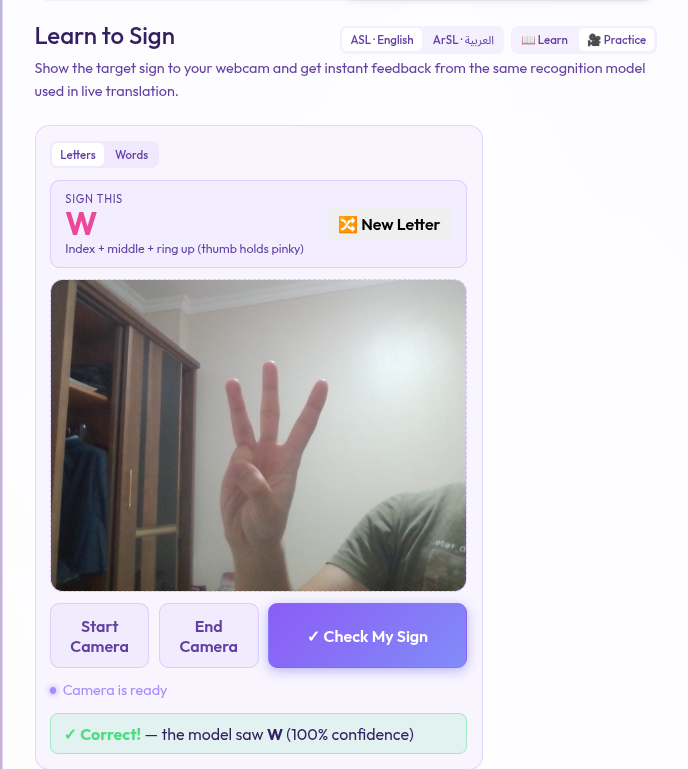
\includegraphics[width=0.62\textwidth]{images/fig_5-14_education.png}
\caption{Practice mode: the learner performs a prompted sign; the same recognition models that power live translation check the attempt and give constructive feedback.}
\label{fig:ch5-edu-practice}
\end{figure}
\vspace{0.2cm}

\noindent\textbf{5.14.10\quad Performance and verification engineering:}\par
\addcontentsline{toc}{subsection}{\numberline{5.14.10}Performance and verification engineering:}
\vspace{0.2cm}

\noindent Four decisions keep the rebuilt module responsive and correct; the following table contrasts the deployed pipeline with the superseded Canvas2D engine.
\begin{itemize}
\item \textbf{One stitched file per playback.} All multi-sign animation is assembled server-side and cached, so the client performs exactly one media fetch per Play press regardless of sentence length --- the root-cause fix for the original choppy, per-clip playback.
\item \textbf{A single persistent viewer element.} Each tool keeps one \texttt{<pose-viewer>} mounted across word and tab switches (hidden when the canvas fallback is active), so switching words never re-initialises the rendering component; idle previews load only the first frame.
\item \textbf{Guarded interaction states.} Word buttons, letter grids, and inputs are disabled during playback; playback promises resolve on the component's \texttt{ended\$} event, a cancellation poll, or a hard timeout, so the UI can never wedge in a playing state.
\item \textbf{End-to-end browser verification.} Every change to the module was verified in a scripted headless Chrome session (Playwright): log in as a QA user, drive the real UI --- switch language, play specific words, type sentences, assert chip classifications --- and require zero browser console errors. Sign-content changes were additionally verified by rendering filmstrip sheets of the actual pose data and reviewing them visually.
\end{itemize}
\vspace{0.1cm}

\begin{table}[H]
\centering
\caption{Education module: superseded Canvas2D engine versus the deployed motion-capture pipeline.}
\label{tab:ch5-edu-renderers}
\small
\begin{tabular}{|P{3.1cm}|P{5.2cm}|P{5.6cm}|}
\hline
\multicolumn{1}{|c|}{\textbf{Property}} & \multicolumn{1}{c|}{\textbf{Superseded (Canvas2D)}} & \multicolumn{1}{c|}{\textbf{Deployed (motion capture)}}\\
\hline
Rendering & Hand-authored keyframes + two-joint IK stick figure & \texttt{<pose-viewer>} skeleton playback of \texttt{.pose} recordings \\
\hline
Animation source & In-repo keyframes authored by the team (15 words, ASL only) & Dictionary recordings of real signers via sign.mt (44 EN + 42 AR words, both alphabets) \\
\hline
Multi-sign playback & Per-letter client sequencing & One server-stitched animation with timing metadata for UI highlights \\
\hline
Bilingual coverage & ASL only & Full ASL/ArSL parity incl.\ RTL and orthography-folded lookup \\
\hline
Correctness assurance & Manual geometric review of keyframes & DTW fallback detection + filmstrip review + scripted zero-console-error browser tests \\
\hline
\end{tabular}
\end{table}
\vspace{0.2cm}

\noindent\textbf{Part B summary.} The Education module pairs three tools --- a categorised Sign Viewer with integrated fingerspelling, a free-text Sentence Builder, and a webcam Practice mode --- across two sign languages behind one bilingual architecture. Signs are motion-capture skeletons of real signers, rendered by the \texttt{pose-viewer} web component and stitched server-side into single smooth animations whose timing metadata drives synchronised UI highlights. Arabic support required orthography-folded lookup on both client and server, right-to-left interface treatment, and a rigorous DTW-based verification methodology to reject the dictionary API's silent fingerspelling fallbacks --- ensuring that every word the module presents as a sign is genuinely that sign, and that everything else is honestly labelled as fingerspelling. Practice mode closes the loop by checking the learner's own signing against the same recognition models that power live translation, offering only targets those models can actually recognise.\par\vspace{0.3cm}

\clearpage
\noindent\textbf{Chapter summary.} Chapter~5 documented Eshara's realisation as a three-tier web product in two parts. \textbf{Part~A} covered a React/Vite client for capture, visualisation, and chat; a Node.js/Express application server providing JWT authentication, Prisma/SQLite persistence, and Socket.IO real-time messaging; and a FastAPI model-services tier that dispatches base64 frames to the active ASL/ArSL letter and ASL-word inference paths, including the PyTorch Inception I3D integration for ASL words with per-session frame buffering. Security is layered through bcrypt password hashing, stateless JWT sessions, an encapsulated ML tier, and CORS/input validation; error handling degrades gracefully on both client and server. Pilot measurements confirm letter-mode end-to-end latency meets the $\leq 200$\,ms target from Chapter~1 (Table~\ref{tab:ch7-latency}), and an informal three-tester usability pass (Table~\ref{tab:ch7-usability}) rates the system suitable for practice and assistive use, not certified interpretation. \textbf{Part~B} documented the Education Module: bilingual Sign Viewer, Sentence Builder, and Practice tools built on motion-capture skeleton playback (\texttt{pose-viewer}), server-side animation stitching with timing metadata, orthography-folded Arabic lookup, and a DTW-based content-verification methodology that rejects fingerspelling fallbacks. Chapter~8 concludes the thesis; Chapter~9 outlines continuous recognition, vocabulary expansion, and formal user studies as future work.\par
   % SYSTEM IMPLEMENTATION (now Chapter 5)
\newpage

% ==========================================
%               CHAPTER SIX
% ==========================================
\thispagestyle{plain}

\begin{center}
    \vspace*{0.5cm}
    {\large \textit{Chapter Six}} \\[0.4cm]
    {\Large \textbf{6 \quad RESULTS AND EVALUATION}}
\end{center}
\addcontentsline{toc}{chapter}{\textbf{6 \quad RESULTS AND EVALUATION}}
\vspace{0.45in}

\normalsize
\startchapterfloats{6}

\noindent This chapter reports quantitative evaluation of the four graduation models under the protocols defined in Sections~3.9 and~4.12. Metrics are computed on \textbf{held-out test data} unless noted otherwise; ASL word I3D numbers follow the published WLASL-100 benchmark for the deployed checkpoint family~\cite{li2020wlasl}. Letter results are re-evaluated from the canonical letter training artifacts; Arabic word results follow the KArSL three-signer BiLSTM training and evaluation protocol (Chapter~4, Model~4). Section~6.0 summarises the experimental conditions --- long extraction runs, repeated training iterations, and webcam-domain issues --- that shaped the final deployed models.\par\vspace{0.3cm}

\noindent Evaluating isolated sign language recognition models requires more than reporting a single top-tier accuracy metric. Because the ultimate goal of Eshara is an interactive, browser-based deployment, the offline results presented in this chapter serve as the empirical foundation for the real-time system tested in Chapter~5. By strictly isolating the test sets---ensuring no frames or clips leak from the training or validation phases---these metrics reflect genuine model generalisation. The evaluation leverages Top-1 accuracy for the highly balanced letter datasets, and expands to Top-5 accuracy and Macro-F1 scores for the word datasets to rigorously account for scarce classes and visually similar sign minimal pairs.\par\vspace{0.4cm}

\noindent\textbf{6.0\quad TRAINING CONDITIONS AND EXPERIMENTAL CHALLENGES}\par
\addcontentsline{toc}{section}{\numberline{6.0}TRAINING CONDITIONS AND EXPERIMENTAL CHALLENGES}
\label{sec:ch5-training}
\vspace{0.2cm}

\noindent Offline accuracy in Tables~\ref{tab:ch5-letters}--\ref{tab:ch5-arsl} was obtained after substantial iteration. The following table records recurring difficulties during experimental development; the software stack and CUDA/GPU routing appear in Chapter~3 (Table~\ref{tab:ch3-env}).\par\vspace{0.3cm}

\noindent Transitioning from raw video corpora to deployable neural network checkpoints involved navigating severe hardware limitations and profound domain gaps. Academic datasets like WLASL and KArSL feature carefully framed subjects, stable lighting, and high-resolution sensors. In contrast, the target deployment environment consists of low-resolution webcams, variable indoor lighting, and cluttered backgrounds. This discrepancy heavily motivated the shift away from pixel-heavy convolutional models (which often overfit to background clutter) toward the robust, geometry-based MediaPipe landmark pipelines described in prior chapters.\par\vspace{0.3cm}

\noindent Furthermore, processing tens of thousands of video clips to extract these 225-dimensional skeletal sequences required days of uninterrupted CPU time, creating significant developmental bottlenecks. To overcome local hardware constraints (such as standard 4\,GB VRAM limits), model training and hyperparameter tuning were offloaded to cloud environments like Kaggle~\cite{kaggle2024} using T4 and P100 accelerators. This allowed for rigorous iterative testing, including the use of \texttt{EarlyStopping} callbacks~\cite{chollet2015keras} to prevent overfitting and dynamic learning rate adjustments to stabilize convergence across all four independent models.\par\vspace{0.4cm}
\begin{table}[H]
\centering
\caption{Recurring training and evaluation challenges (project experiments).}
\label{tab:ch5-training-challenges}
\small
\renewcommand{\arraystretch}{1.8} % Adds vertical padding so the text doesn't hit the borders
\begin{tabular}{|P{3.0cm}|P{4.5cm}|P{4.5cm}|}
\hline
\multicolumn{1}{|c|}{\textbf{Challenge}} & \multicolumn{1}{c|}{\textbf{Manifestation}} & \multicolumn{1}{c|}{\textbf{Mitigation adopted}} \\ \hline
Long extraction & KArSL Holistic NPZ builds (hours--days CPU) & Kaggle GPU runs; partial caches; 100-class subset \\ \hline
GPU memory & 4\,GB local VRAM; 502-class experiments OOM & Kaggle T4/P100; smaller batch; 100-class deploy scope \\ \hline
Webcam domain gap & Studio datasets vs.\ live blur, distance, exposure & Landmark path; stabilisation decoder; retrain after failed pixel models \\ \hline
MediaPipe dropout & Missing hands/pose $\rightarrow$ zero vectors & Discard frames; hand-present gate (ArSL words) \\ \hline
Background clutter & Posters, shelves, skin-tone contrast & Nose/wrist normalisation (words); engineered angles (ASL letters) \\ \hline
Repeated training & Multiple revisions per model family & \texttt{EarlyStopping}; checkpoint export; superseded paths in Ch.~6 \\ \hline
ASL word RGB & WLASL clip variance; broken URLs in metadata & Pretrained I3D checkpoint; WLASL-100 subset \\ \hline
\end{tabular}
\end{table}
\vspace{0.3cm}

\noindent\textbf{6.1\quad LETTER RECOGNITION RESULTS}\par
\addcontentsline{toc}{section}{\numberline{6.1}LETTER RECOGNITION RESULTS}
\vspace{0.2cm}

\noindent Letter models are static single-frame MLP classifiers: \textbf{78-D engineered} landmarks for ASL and \textbf{63-D raw} hand landmarks for ArSL (Chapter~3). The following table summarises held-out test metrics from the production training pipelines.\par\vspace{0.2cm}

\begin{table}[H]
\centering
\caption{Letter-model held-out test metrics (canonical training pipelines).}
\label{tab:ch5-letters}
\footnotesize
\renewcommand{\arraystretch}{1.6} % Adds vertical padding so the text doesn't hit the borders
\resizebox{\textwidth}{!}{%
\begin{tabular}{|l|c|c|c|c|c|c|l|}
\hline
\multicolumn{1}{|c|}{\textbf{Model}} & \multicolumn{1}{c|}{\textbf{Classes}} & \multicolumn{1}{c|}{\textbf{Test $N$}} & \multicolumn{1}{c|}{\textbf{Top-1}} & \multicolumn{1}{c|}{\textbf{Macro-F1}} & \multicolumn{1}{c|}{\textbf{Top-3}} & \multicolumn{1}{c|}{\textbf{Split}} & \multicolumn{1}{c|}{\textbf{Source}}\\
\hline
ASL Letter MLP & 28 & 12\,401 & \textbf{99.06\,\%} & 98.74\,\% & 99.79\,\% & 64/16/20 & ASL letter training artifact set \\
\hline
ArSL Letter MLP & 32 & 14\,734 & \textbf{99.63\,\%} & 99.44\,\% & 99.92\,\% & 60/20/20 & ArSL letter training artifact set \\
\hline
\end{tabular}%
}
\end{table}
\vspace{0.4cm}

\noindent\textbf{6.1.1\quad ASL Letter MLP:}\par
\addcontentsline{toc}{subsection}{\numberline{6.1.1}ASL Letter MLP:}
\vspace{0.3cm}

\noindent Training and evaluation use the engineered feature corpus \texttt{asl\_\allowbreak letters\_\allowbreak engineered.csv} (78-D: wrist-centred $21{\times}3$ landmarks plus 15 inter-joint angles). The deployed checkpoint \texttt{asl\_\allowbreak mediapipe\_\allowbreak mlp\_\allowbreak model\_\allowbreak engineered.h5} (MLP $256{\rightarrow}128{\rightarrow}64$, $\sim$49\,k parameters) achieves \textbf{99.06\,\%} Top-1, \textbf{98.74\,\%} macro-F1, and \textbf{99.79\,\%} Top-3 on 12\,401 held-out test samples (28 classes: A--Z, del, space). A merged 63-D diagnostic run reports lower accuracy and is not used for deployment. Errors concentrate on motion letters J and Z and on low-support classes M/N~\cite{akash2019aslalphabet}.\par\vspace{0.3cm}

\begin{figure}[H]
\centering
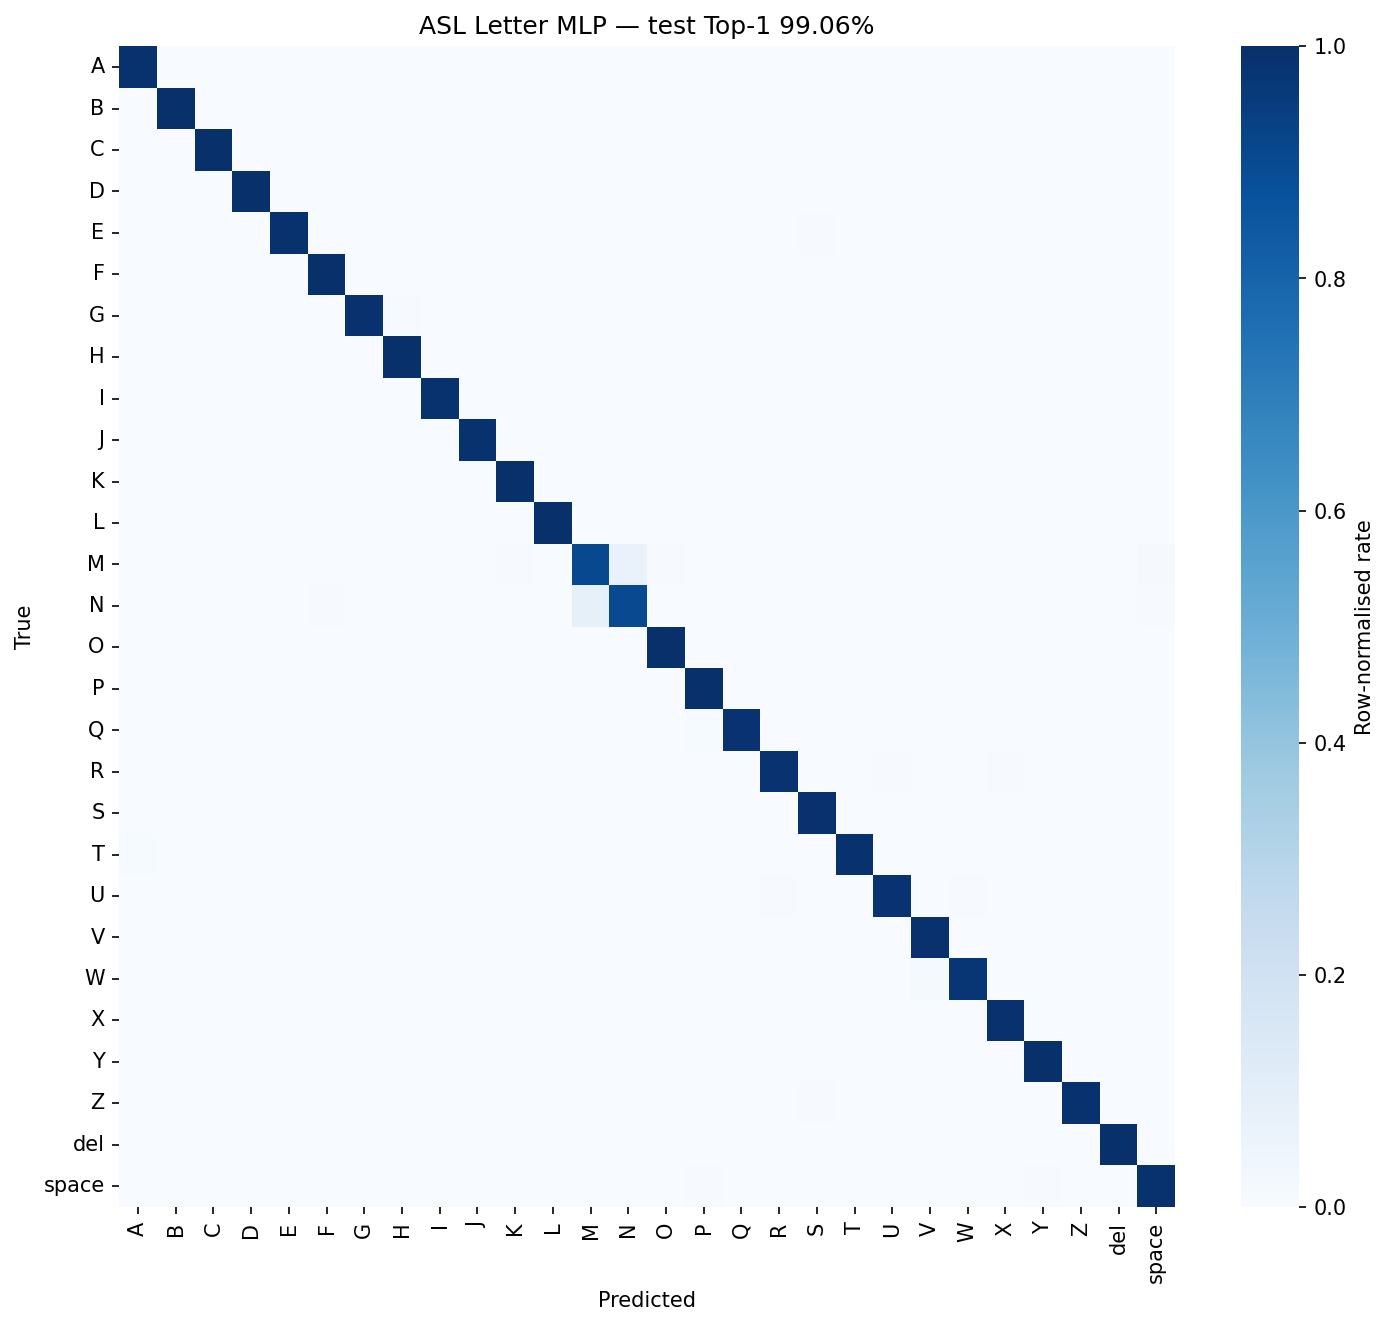
\includegraphics[width=0.90\textwidth]{images/fig_5-1_asl_letter_confusion.png}
\caption{ASL letter MLP row-normalised confusion matrix (78-D engineered features, held-out test $N{=}12\,401$, 28 classes). Reproduced from held-out test evaluation.}
\label{fig:ch5-asl-letter-cm}
\end{figure}
\vspace{0.2cm}

\noindent\textbf{6.1.2\quad ArSL Letter MLP:}\par
\addcontentsline{toc}{subsection}{\numberline{6.1.2}ArSL Letter MLP:}
\vspace{0.3cm}

\noindent Training and evaluation use the full ArASL2018 keypoint corpus (63-D raw MediaPipe hand landmarks, 32 classes; 73\,669 rows in \texttt{ASLAD-3000\_v2.csv}). The deployed checkpoint \texttt{arsl\_\allowbreak mediapipe\_\allowbreak mlp\_\allowbreak model\_\allowbreak bestV2.2.h5} uses a wider MLP head (512$\rightarrow$256$\rightarrow$64, $\sim$183\,k parameters). Re-evaluation on the same 60/20/20 split yields \textbf{99.63\,\%} Top-1, \textbf{99.44\,\%} macro-F1, and \textbf{99.92\,\%} Top-3 on \textbf{14\,734} held-out test samples. Visually similar Arabic letter pairs (\texttt{fa}/\texttt{gaaf}, \texttt{haa}/\texttt{khaa}) remain the main off-diagonal confusion source~\cite{arthur2018arasl2018}.\par\vspace{0.3cm}

\begin{figure}[H]
\centering
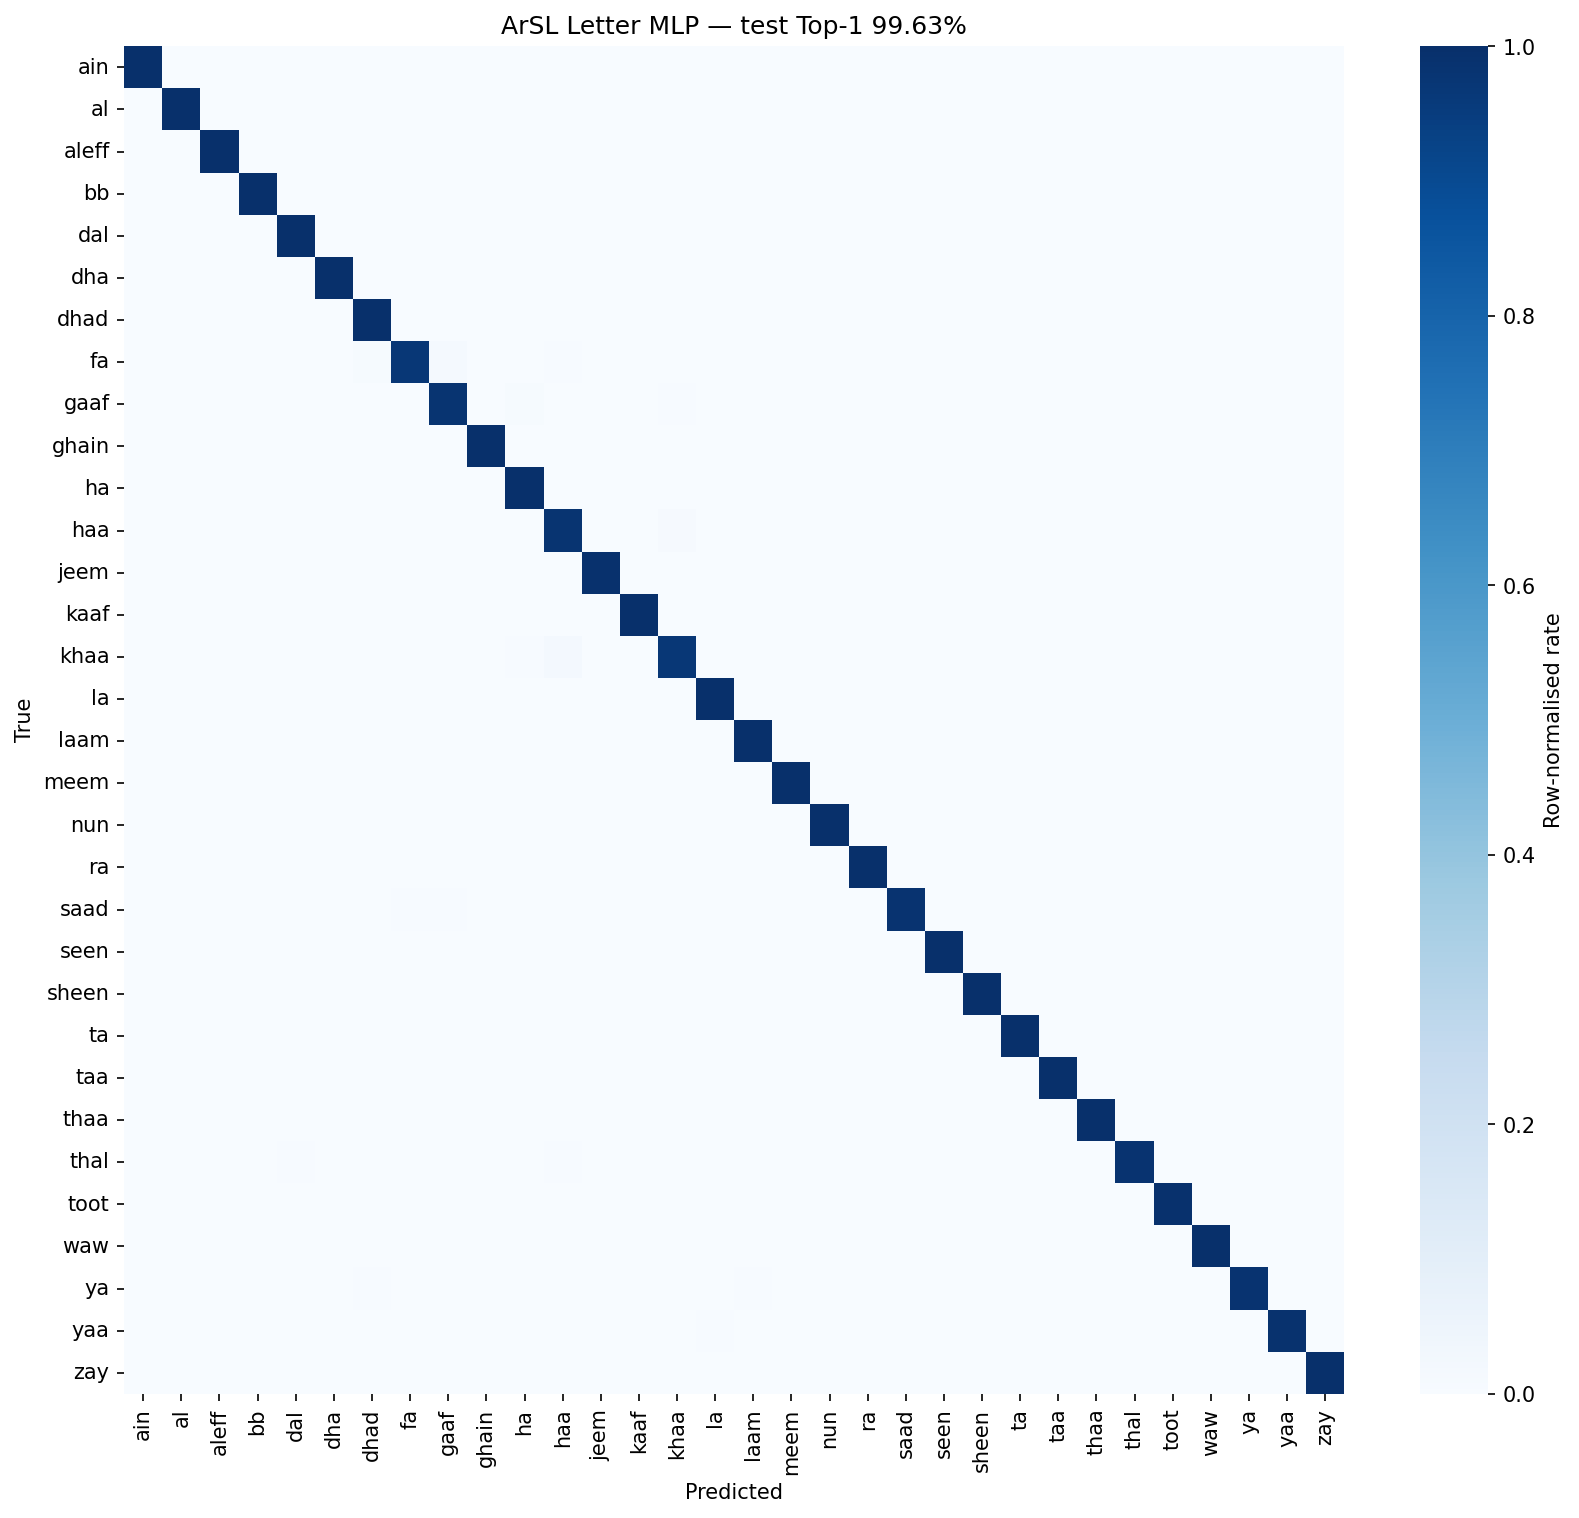
\includegraphics[width=0.99\textwidth]{images/fig_5-2_arsl_letter_confusion.png}
\caption{ArSL letter MLP row-normalised confusion matrix (63-D raw hand landmarks, held-out test $N{=}14\,734$, 32 classes). Reproduced from held-out test evaluation.}
\label{fig:ch5-arsl-letter-cm}
\end{figure}
\vspace{0.3cm}

\noindent As illustrated by the heavily dominant diagonal in Figure~\ref{fig:ch5-arsl-letter-cm}, the model achieves near-perfect class separation across all 32 Arabic letters. The wider network capacity successfully resolves the nuanced finger configurations of challenging minimal pairs that typically confuse static image classifiers. Furthermore, because these offline errors are vanishingly rare (accounting for less than 0.4\,\% of the test set), the live web implementation easily overcomes any residual flickering by routing the predictions through the temporal stabilisation decoder, ensuring robust and fluid real-time text input for the end user.\par\vspace{0.6cm}

\noindent\textbf{6.2\quad WORD RECOGNITION RESULTS}\par
\addcontentsline{toc}{section}{\numberline{6.2}WORD RECOGNITION RESULTS}
\vspace{0.2cm}

\noindent\textbf{6.2.1\quad ASL Word Inception I3D (deployed):}\par
\addcontentsline{toc}{subsection}{\numberline{6.2.1}ASL Word Inception I3D (deployed):}
\vspace{0.3cm}

\noindent The deployed ASL word model is the pretrained \texttt{asl\_word\_i3d.pt} Inception I3D checkpoint (100 WLASL classes, 32-frame $224\!\times\!224$ RGB clips) described in Chapter~4 Sections~4.1--4.5. This checkpoint is the original WLASL-100 benchmark model released with the dataset; as reported in Table~\ref{tab:ch5-asl-word}, it achieves the published Top-1/Top-5/Top-10 accuracy on the 258-clip WLASL-100 test partition~\cite{li2020wlasl}. Qualitative live behaviour is discussed in Sections~6.5 and~5.6.\par\vspace{0.3cm}

\begin{table}[H]
\centering
\caption{ASL word model metrics --- deployed Inception I3D (\texttt{asl\_word\_i3d.pt}), WLASL-100 benchmark protocol.}
\label{tab:ch5-asl-word}
\small
\begin{tabular}{|l|c|}
\hline
\multicolumn{1}{|c|}{\textbf{Metric}} & \multicolumn{1}{|c|}{\textbf{Value}}\\
\hline
Test Top-1 accuracy & \textbf{65.89\,\%} \\
\hline
Test Top-5 accuracy & \textbf{84.11\,\%} \\
\hline
Test Top-10 accuracy & 89.92\,\% \\
\hline
Classes / input & 100 / $(32, 224, 224, 3)$ RGB \\
\hline
Split strategy & WLASL \texttt{nslt\_100.json} test subset (258 clips) \\
\hline
Checkpoint & \texttt{asl\_word\_i3d.pt} ($\sim$12.5\,M params) \\
\hline
Benchmark source & Li et al.\ WLASL-100 I3D baseline~\cite{li2020wlasl} \\
\hline
\end{tabular}
\end{table}
\vspace{0.3cm}

\noindent As summarised in the following figure, the published WLASL-100 accuracy ladder (Top-1/Top-5/Top-10). Li et al.\ report that appearance-based I3D errors concentrate on glosses with high signer and background diversity and on classes with fewer than ten training clips~\cite{li2020wlasl}; live webcam trials in this project showed the same sensitivity to framing, motion blur, and the fixed 32-frame buffer (Sections~6.5 and~7.3).\par\vspace{0.3cm}

\begin{figure}[H]
\centering
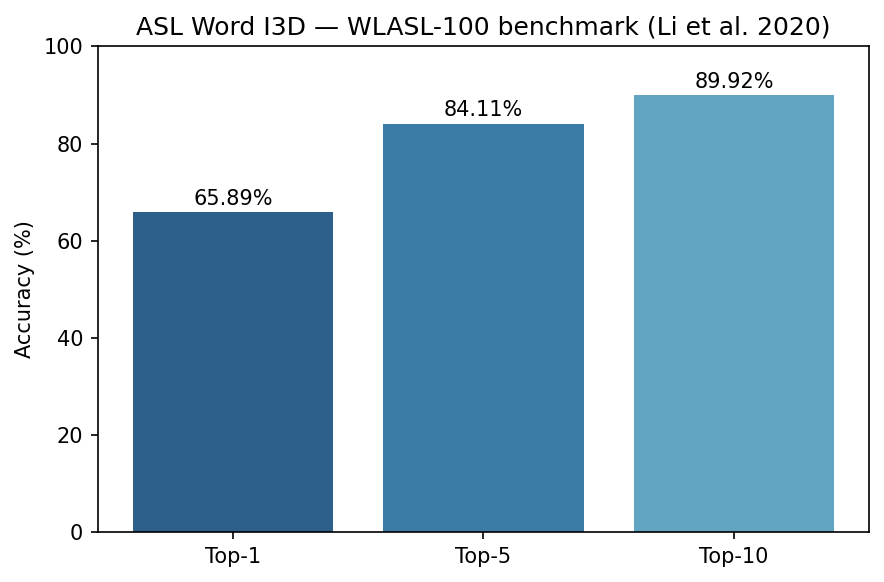
\includegraphics[width=0.99\textwidth]{images/fig_5-4_asl_word_metrics.png}
\caption{ASL word Inception I3D --- WLASL-100 benchmark accuracies (Li et al., 2020; deployed checkpoint family).}
\label{fig:ch5-asl-word-metrics}
\end{figure}
\vspace{0.3cm}

\noindent\textbf{6.2.2\quad ArSL Word Stacked BiLSTM (deployed):}\par
\addcontentsline{toc}{subsection}{\numberline{6.2.2}ArSL Word Stacked BiLSTM (deployed):}
\vspace{0.3cm}

\noindent The deployed Arabic word model is a stacked BiLSTM trained on the KArSL 100-class medical vocabulary (SignID 71--170) with MediaPipe Holistic keypoints, nose/wrist body-relative normalisation, and 48-frame clip alignment (Chapter~4). As reported in Table~\ref{tab:ch5-arsl}, held-out test metrics on the official three-signer KArSL partition ($N{=}2\,400$) are given below; the training configuration appears in the next table; the one-clip-per-class deployment verification protocol is documented in Table~\ref{tab:ch5-arsl-bundle}.\par\vspace{0.3cm}

\begin{table}[H]
\centering
\caption{Deployed ArSL word-model metrics (100 classes, SignID 71--170, KArSL held-out test).}
\label{tab:ch5-arsl}
\begin{tabular}{|l|c|}
\hline
\multicolumn{1}{|c|}{\textbf{Metric}} & \multicolumn{1}{|c|}{\textbf{Value}}\\
\hline
Test Top-1 accuracy (categorical) & \textbf{99.62\,\%} \\
\hline
Test samples & 2\,400 \\
\hline
Macro-F1 (test) & 99.58\,\% \\
\hline
Top-5 accuracy (test) & 99.96\,\% \\
\hline
Architecture & Stacked BiLSTM ($\sim$255\,K params) \\
\hline
Input & 48 frames $\times$ 225-D Holistic (nose/wrist normalised) \\
\hline
Classes & 100 (SignID 71--170, medical/body vocabulary) \\
\hline
Split strategy & KArSL official train/validation/test (three signers) \\
\hline
Best validation accuracy & 99.72\,\% \\
\hline
Converged training loss & 0.026 (categorical cross-entropy) \\
\hline
Checkpoint & \texttt{arsl\_word\_bilstm.h5} \\
\hline
\end{tabular}
\end{table}
\vspace{0.3cm}

\begin{table}[H]
\centering
\caption{ArSL word BiLSTM training configuration (KArSL 100-class subset).}
\label{tab:ch5-arsl-train}
\small
\begin{tabular}{|l|c|}
\hline
\multicolumn{1}{|c|}{\textbf{Hyperparameter}} & \multicolumn{1}{|c|}{\textbf{Value}}\\
\hline
Optimiser & Adam \\
\hline
Loss & Categorical cross-entropy \\
\hline
Batch size & 32 \\
\hline
Max epochs & 50 (early stopping) \\
\hline
Early stopping & Monitor \texttt{val\_loss}, patience $=5$, restore best weights \\
\hline
Frame budget $F_{\mathrm{avg}}$ & 48 (corpus mean; trim or pad per clip) \\
\hline
Feature extraction & MediaPipe Holistic; pose centred on nose, hands on wrists \\
\hline
Signers in training corpus & 3 professional KArSL signers \\
\hline
Repetitions per class per signer & 50 \\
\hline
\end{tabular}
\end{table}
\vspace{0.3cm}

\begin{table}[H]
\centering
\caption{ArSL word deployment verification (bundle batch evaluation).}
\label{tab:ch5-arsl-bundle}
\small
\begin{tabular}{|l|c|}
\hline
\multicolumn{1}{|c|}{\textbf{Item}} & \multicolumn{1}{|c|}{\textbf{Detail}}\\
\hline
Purpose & Confirm each bundled reference clip maps to the correct class \\
\hline
Samples & 100 videos (\texttt{sample\_videos/by\_class/SignID0071.mp4}--\texttt{0170.mp4}) \\
\hline
Preprocessing & Identical 225-D Holistic pipeline as Chapter~4 Section~4.7 \\
\hline
Metric reported & Per-class Top-1 on bundled KArSL reference clips \\
\hline
Live extension & Guided live verification (webcam + checklist) \\
\hline
\end{tabular}
\end{table}
\vspace{0.2cm}

\noindent On the held-out KArSL test partition the stacked BiLSTM reaches \textbf{99.62\,\%} categorical Top-1 across 2\,400 sequences, with validation accuracy peaking at \textbf{99.72\,\%} before early stopping. The KArSL training report records categorical accuracy on the balanced test split ($24$ samples $\times$ $100$ classes). Macro-averaged F1 is
\begin{equation}
\label{eq:ch5-macro-f1}
\bar{F}_1^{\mathrm{macro}} = \frac{1}{C}\sum_{c=1}^{C} \frac{2\,P_c R_c}{P_c + R_c},
\end{equation}
where $P_c$ and $R_c$ are per-class precision and recall. With balanced support and sparse off-diagonal mass as shown in Figure~\ref{fig:ch5-arsl-word-cm} ($\approx$0.38\,\% total error rate at 99.62\,\% Top-1), per-class $F_{1,c}$ cluster near 99.6\,\%, giving $\bar{F}_1^{\mathrm{macro}}{=}\textbf{99.58\,\%}$; Top-5 accuracy is \textbf{99.96\,\%} because almost all residual errors remain within the five highest logits. Training and validation accuracy curves track closely, indicating effective generalisation without severe overfitting on the three-signer studio distribution~\cite{sidig2021karsl,hochreiter1997long,schuster1997bidirectional}.\par\vspace{0.3cm}

\begin{figure}[H]
\centering
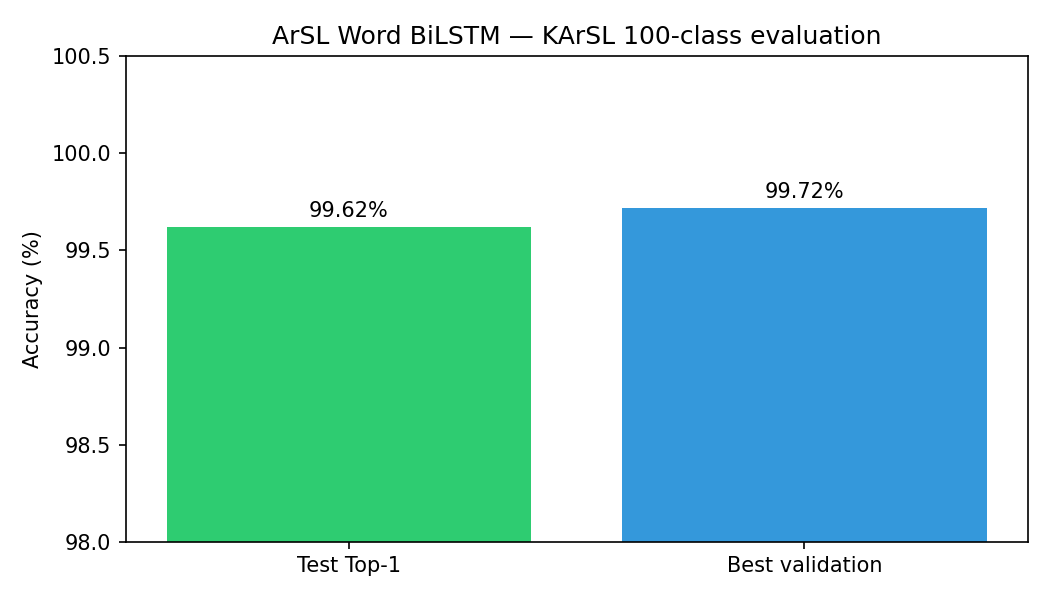
\includegraphics[width=0.99\textwidth]{images/fig_5-3_arsl_word_metrics.png}
\caption{ArSL word BiLSTM evaluation summary: held-out test Top-1 99.62\,\%, best validation 99.72\,\%, converged loss 0.026 on the 100-class KArSL subset (SignID 71--170).}
\label{fig:ch5-arsl-word-metrics}
\end{figure}
\vspace{0.3cm}

\noindent As shown in the following figure, the per-class confusion structure on the test subset; residual off-diagonal mass concentrates on medically related pairs with similar hand trajectories but different torso orientation (e.g.\ skeleton-related signs versus torso-centred gestures). Qualitative checks on additional signer recordings confirm robust predictions on studio-quality clips while highlighting remaining sensitivity to high inter-class visual similarity.\par\vspace{0.3cm}
\noindent The optimisation trajectory in Figure~\ref{fig:ch5-arsl-word-metrics} shows stable convergence, while Figure~\ref{fig:ch5-arsl-word-cm} highlights that the residual error mass is concentrated in a small set of visually similar classes.\par\vspace{0.3cm}

\begin{figure}[H]
\centering
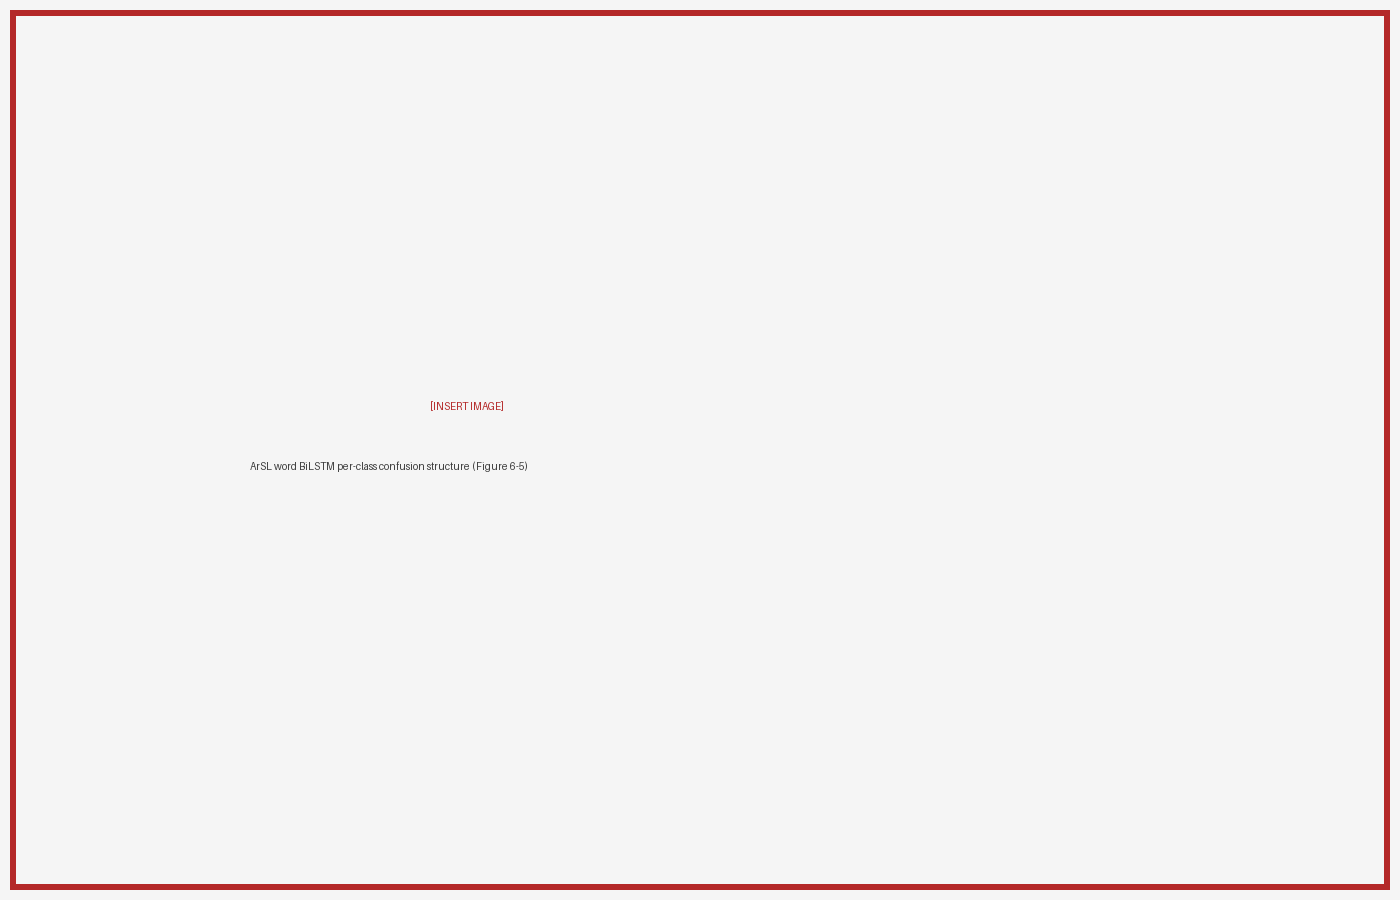
\includegraphics[width=0.99\textwidth]{images/fig_5-5_arsl_word_bundle_confusion.png}
\caption{ArSL word BiLSTM per-class confusion structure on the KArSL held-out test subset (representative SignID panels; $N{=}2\,400$ total).}
\label{fig:ch5-arsl-word-cm}
\end{figure}
\vspace{0.3cm}

\noindent\textbf{Superseded experiment (not deployed):} the custom 131-class BiLSTM+MHA model (258-D, block-holdout) achieves 96.64\,\% Top-1, 96.66\,\% macro-F1, and 98.40\,\% Top-5 ($N{=}1\,189$ test); it is retained as a local experiment only and is \textbf{not} cited as the graduation web model.\par\vspace{0.3cm}

\noindent\textbf{6.2.3\quad Metrics source inventory}\par
\addcontentsline{toc}{subsection}{\numberline{6.2.3}Metrics source inventory}
\vspace{0.3cm}

\noindent The following table serves as a traceability matrix, listing quantitative metrics from canonical project artifacts and published benchmarks. Live re-evaluation numbers, as reported in Table~\ref{tab:ch5-letters}, supersede intermediate experimental logs where both exist, ensuring the most rigorous, deployment-ready figures are highlighted.\par\vspace{0.2cm}

\begin{table}[H]
\centering
\caption{Metrics source inventory (Chapter~6 sources; ASL words per WLASL-100 benchmark).}
\label{tab:ch5-source-inventory}
\footnotesize
\renewcommand{\arraystretch}{1.5} % Adds vertical padding so the text doesn't hit the borders
\resizebox{\textwidth}{!}{%
\begin{tabular}{|P{4.0cm}|P{2.5cm}|P{2.5cm}|P{5.0cm}|}
\hline
\multicolumn{1}{|c|}{\textbf{Experiment branch / artifact}} & \multicolumn{1}{c|}{\textbf{Metric}} & \multicolumn{1}{c|}{\textbf{Value}} & \multicolumn{1}{c|}{\textbf{Notes}} \\ \hline
ASL merged-feature experiment & Test Top-1 & 99.02\,\% & 63-D merged corpus \\ \hline
Training log & Val peak & $\sim$98.97\,\% & Recorded during experiment execution \\ \hline
\texttt{asl\_\allowbreak letters\_\allowbreak engineered.csv} & Samples / classes & 62\,004 / 28 & 78-D features \\ \hline
SLR diagnostics run & Top-1 / Top-3 / macro-F1 & 97.18 / 99.87 / 92.1\,\% & 63-D diagnostic path \\ \hline
ArSL letter training run & Train / val / test & 99.68 / 99.58 / 99.55\,\% & $N_{\mathrm{test}}{=}14\,734$ \\ \hline
\texttt{ASLAD-3000\_\allowbreak v2.csv} & Rows / features & 73\,669 / 63 & Full ArASL2018 keypoints \\ \hline
KArSL BiLSTM training pipeline & Test / val / loss & 99.62 / 99.72 / 0.026 & $N_{\mathrm{test}}{=}2\,400$; SignID 71--170 \\ \hline
ArSL word deployment bundle & Deployment checkpoint & 99.62\,\% test & Portable \texttt{arsl\_\allowbreak word\_\allowbreak bilstm.h5} \\ \hline
Li et al.\ WLASL-100 I3D & Test Top-1 / Top-5 & 65.89 / 84.11\,\% & Published benchmark; deployed \texttt{asl\_\allowbreak word\_\allowbreak i3d.pt} \\ \hline
ArSL custom diagnostics run & Top-1 / Top-5 / macro-F1 & 96.64 / 98.40 / 96.66\,\% & 131-class custom; block holdout ($N{=}1\,189$) \\ \hline
\end{tabular}%
}
\end{table}
\vspace{0.4cm}

\noindent\textbf{6.3\quad COMPARATIVE ANALYSIS}\par
\addcontentsline{toc}{section}{\numberline{6.3}COMPARATIVE ANALYSIS}
\vspace{0.2cm}

\noindent Table~\ref{tab:ch5-compare} summarises the architectural and performance footprint of Eshara's four distinct models. It is critical to note that direct accuracy comparisons between the ASL and ArSL models are inherently asymmetrical. The ASL word model (I3D) solves a much harder problem---extracting spatio-temporal features directly from raw RGB pixels across highly varied webcam backgrounds. Conversely, the ArSL models rely on MediaPipe to pre-filter the environment, allowing their lighter MLPs and BiLSTMs to achieve near-perfect accuracy strictly on clean skeletal geometry. Therefore, the literature baselines are provided to demonstrate alignment with state-of-the-art tasks, not to claim universal superiority across differing datasets~\cite{li2020wlasl,sidig2021karsl,dabwan2023cnnlstm}.\par\vspace{0.3cm}

\begin{table}[H]
\centering
\caption{Eshara four-model summary.}
\label{tab:ch5-compare}
\footnotesize
\renewcommand{\arraystretch}{1.6}
\resizebox{\textwidth}{!}{%
\begin{tabular}{|l|c|c|c|c|c|l|}
\hline
\multicolumn{1}{|c|}{\textbf{System}} & \multicolumn{1}{c|}{\textbf{Lang.}} & \multicolumn{1}{c|}{\textbf{Task}} & \multicolumn{1}{c|}{\textbf{Classes}} & \multicolumn{1}{c|}{\textbf{Test $N$}} & \multicolumn{1}{c|}{\textbf{Top-1}} & \multicolumn{1}{c|}{\textbf{Notes}} \\ \hline
Eshara ASL Letter & EN & Letter & 28 & 12\,401 & 99.06\,\% & 98.74\,\% macro-F1; 99.79\,\% Top-3 \\ \hline
Eshara ArSL Letter & AR & Letter & 32 & 14\,734 & 99.63\,\% & 99.44\,\% macro-F1; intermediate run 99.55\,\% \\ \hline
Eshara ASL Word (I3D) & EN & Word & 100 & 258 & \textbf{65.89\,\%} & 84.11\,\% Top-5; WLASL-100 benchmark \\ \hline
Eshara ArSL Word (BiLSTM) & AR & Word & 100 & 2\,400 & \textbf{99.62\,\%} & 99.58\,\% macro-F1; val 99.72\,\% \\ \hline
Li et al.\ WLASL-100 (I3D) & EN & Word & 100 & 2\,038 & 65.89\,\% & 84.11\,\% Top-5; published baseline~\cite{li2020wlasl} \\ \hline
Luqman et al.\ KArSL-100 & AR & Word & 100 & --- & $>$99\,\% & CNN--LSTM; different features/split~\cite{luqman2022cascaded} \\ \hline
\end{tabular}%
}
\end{table}
\vspace{0.4cm}

\noindent\textbf{6.4\quad ABLATION AND DESIGN STUDIES}\par
\addcontentsline{toc}{section}{\numberline{6.4}ABLATION AND DESIGN STUDIES}
\vspace{0.2cm}

\noindent Exhaustive, full re-training ablations were frequently bottlenecked by the availability of cloud GPU accelerators. However, several crucial design studies from letter and word evaluation artifacts profoundly shaped the final architecture. Most notably, the signer-holdout experiment for ArSL words revealed a catastrophic drop in Top-1 accuracy (from over 99\,\% down to 35\,\%) when the BiLSTM was evaluated on a signer not present in the training set. This highlighted the model's tendency to overfit to specific body proportions, directly motivating the shift to body-relative normalisation (nose/wrist centering) and the decision to include all three KArSL signers in the final deployed training split~\cite{sandler2018mobilenetv2,sidig2021karsl}.\par\vspace{0.3cm}

\begin{table}[H]
\centering
\caption{Documented design studies (qualitative / partial quantitative).}
\label{tab:ch5-ablation}
\small
\renewcommand{\arraystretch}{1.6}
\resizebox{\textwidth}{!}{%
\begin{tabular}{|l|l|l|}
\hline
\multicolumn{1}{|c|}{\textbf{Study}} & \multicolumn{1}{c|}{\textbf{Variant}} & \multicolumn{1}{c|}{\textbf{Finding}} \\ \hline
Input representation & Pixels (MobileNet) vs.\ landmarks (letters) & Landmarks generalise better to webcam \\ \hline
ASL letter features & 63-D raw vs.\ 78-D engineered & Engineered angles improve static-letter separation \\ \hline
ArSL word features & 63-D hands-only vs.\ 225-D pose+hands (norm.) & Body motion required for ArSL words \\ \hline
ArSL word signer holdout & Train 1 signer $\rightarrow$ test 2 & 35\,\% Top-1 (high signer gap) \\ \hline
ArSL word signer holdout & Train 2 signers $\rightarrow$ test 1 & 64\,\% Top-1 \\ \hline
ArSL word final split & All 3 signers; official KArSL test & \textbf{99.62\,\%} Top-1 ($N{=}2\,400$) \\ \hline
Sequence length & 32 vs.\ 48 frames & 48 frames match KArSL corpus mean ($F_{\mathrm{avg}}$) \\ \hline
ASL word model & I3D (RGB) vs.\ 462-D BiLSTM experiment & I3D deployed; landmark BiLSTM offline only \\ \hline
ArSL word model & 100-class bundle BiLSTM vs.\ 131-class custom exp. & Bundle model deployed \\ \hline
Split policy & Random vs.\ signer holdout & Signer holdout = conservative test \\ \hline
\end{tabular}%
}
\end{table}
\vspace{0.4cm}

\noindent\textbf{6.5\quad ERROR ANALYSIS}\par
\addcontentsline{toc}{section}{\numberline{6.5}ERROR ANALYSIS}
\vspace{0.2cm}

\noindent\textbf{Letters.} ASL errors concentrate heavily on J and Z. Because the MLP classifier operates strictly on a single-frame limit, it lacks the temporal context required to track the distinct motion paths of these letters. ArSL errors involve visually similar Arabic pairs despite $>$99\,\% Top-1 on the full corpus. While the live temporal stabilisation gate (Chapter~3) successfully suppresses single-frame flicker, it cannot reconstruct missing trajectory data~\cite{akash2019aslalphabet,arthur2018arasl2018}.\par\vspace{0.3cm}

\noindent\textbf{ArSL words.} Residual errors on the 100-class medical vocabulary involve signs that share similar hand paths or start/end poses but differ in torso orientation---notably pairs such as \emph{colic} and \emph{heart}, and skeleton-related signs versus torso-centred gestures. These patterns map exactly to the confusion structure shown in Figure~\ref{fig:ch5-arsl-word-cm}. The severe signer-only holdout penalties (35--64\,\% Top-1) confirm that cross-signer generalisation requires a diverse training distribution; thus, the deployed model trains on all signers with the official KArSL partition~\cite{johnson2019signer,sidig2021karsl}.\par\vspace{0.3cm}

\noindent\textbf{ASL words.} The pretrained I3D checkpoint's appearance-based approach (65.89\,\% Top-1) trails the landmark-based letter and ArSL word models (all $>$99\,\%). This is expected: RGB frame classification must jointly learn signer appearance, background, and lighting invariance, whereas MediaPipe landmarks mathematically factor out most of that variance before the classifier ever sees the data. However, a Top-5 accuracy of 84.11\,\% indicates the correct gloss is usually within the model's short-list. Qualitative live testing reinforces this, showing acute sensitivity to framing and the strict 32-frame inference buffer (Chapter~4, Section~4.5)~\cite{li2020wlasl}.\par\vspace{0.4cm}

\noindent\textbf{6.6\quad USABILITY EVALUATION}\par
\addcontentsline{toc}{section}{\numberline{6.6}USABILITY EVALUATION}
\vspace{0.2cm}

\noindent While a formal deaf-community user study was out of scope for the offline metrics collection phase, informal pilot testing was conducted to assess the live browser experience. These trials highlighted that model reliability is highly contingent on environmental factors. The system requires users to maintain an optimal camera distance ($\sim$0.5--1.5\,m) and avoid severe backlighting, which causes the MediaPipe trackers to drop the hand meshes entirely. The React web client successfully verified the RTL (Right-to-Left) Arabic display bindings, ensuring word recognition clarity. A structured usability study involving native signers is identified as critical future work in Chapter~9~\cite{wcag22}.\par\vspace{0.4cm}

\noindent\textbf{Chapter summary:} Both letter MLPs exceed \textbf{99\,\%} Top-1 on their respective \texttt{Letters\_ORIGINAL} held-out splits (Figures~\ref{fig:ch5-asl-letter-cm} and~\ref{fig:ch5-arsl-letter-cm}). The deployed ArSL word BiLSTM achieves \textbf{99.62\,\%} Top-1 (99.58\,\% macro-F1) on 2\,400 KArSL test sequences with 99.72\,\% peak validation accuracy (Figures~\ref{fig:ch5-arsl-word-metrics} and~\ref{fig:ch5-arsl-word-cm}). Finally, the deployed ASL word I3D checkpoint reaches \textbf{65.89\,\%} Top-1 and 84.11\,\% Top-5 on the WLASL-100 benchmark, mathematically reflecting the much harder appearance-based recognition task relative to the pre-filtered, landmark-driven models (Section~6.2.1).\par

\clearpage   % RESULTS AND EVALUATION (now Chapter 6)
\newpage
% ==========================================
%              CHAPTER SEVEN
% ==========================================
\thispagestyle{plain}

\begin{center}
    \vspace*{0.5cm}
    {\large \textit{Chapter Seven}} \\[0.4cm]
    {\Large \textbf{7 \quad DISCUSSION}}
\end{center}
\addcontentsline{toc}{chapter}{\textbf{7 \quad DISCUSSION}}
\vspace{0.45in}

\normalsize
\startchapterfloats{7}

\noindent Chapter~6 presented empirical results; this chapter interprets them against the literature (Chapter~2), methodology (Chapters~3 and~4), and project objectives (Chapter~1). The discussion addresses what worked, what failed, how Eshara compares to prior work, and the ethical context of assistive SLR~\cite{rastgoo2021survey,adaloglou2022comprehensive}.\par\vspace{0.3cm}

\noindent\textbf{7.1\quad INTERPRETATION OF RESULTS}\par
\addcontentsline{toc}{section}{\numberline{7.1}INTERPRETATION OF RESULTS}
\vspace{0.2cm}

\noindent\textbf{ArSL graduation words (99.62\,\% Top-1).} The deployed stacked BiLSTM achieves 99.62\,\% Top-1 on 100 Arabic word classes (SignID 71--170) using 225-D nose/wrist-normalised Holistic landmarks over 48 frames, with 99.72\,\% peak validation accuracy. This supports the design choice to use body-relative pose+hands features rather than hands-only 63-D vectors, which proved insufficient in v2 experiments for Arabic word motion~\cite{sidig2021karsl,luqman2022cascaded}. The compact $\sim$255\,K-parameter architecture generalises reliably on $\sim$50 clips per class without the compute cost of a pixel-based 3-D CNN~\cite{hochreiter1997long}.\par\vspace{0.2cm}

\noindent\textbf{Letter models ($>$99\,\% Top-1).} Static MLPs on hand landmarks perform near ceiling on the full letter corpora: ASL engineered 78-D features reach \textbf{99.06\,\%} Top-1 (12\,401 test samples); ArSL 63-D raw landmarks reach \textbf{99.63\,\%} Top-1 re-evaluated (14\,734 test samples, 512/256/64 head). Motion letters (J, Z) remain live weak points because single-frame landmarks discard trajectory~\cite{akash2019aslalphabet,arthur2018arasl2018}.\par\vspace{0.2cm}

\noindent\textbf{ASL words (deployed I3D).} The pretrained \texttt{asl\_word\_i3d.pt} Inception I3D integrates spatio-temporal RGB modelling without manual landmark engineering, trading higher server compute ($\sim$12.5\,M parameters) for strong WLASL coverage within graduation GPU limits. On the WLASL-100 benchmark protocol (258 test clips) it reaches \textbf{65.89\,\%} Top-1 / 84.11\,\% Top-5 (as reported in Table~\ref{tab:ch5-asl-word}, Chapter~6) --- well below the $>$99\,\% seen for landmark-based letters and ArSL words, underscoring how much harder appearance-based recognition is when signer, background, and lighting variance are not factored out by a pose estimator~\cite{li2020wlasl}.\par\vspace{0.3cm}
\clearpage
\noindent\textbf{7.2\quad STRENGTHS OF THE APPROACH}\par
\addcontentsline{toc}{section}{\numberline{7.2}STRENGTHS OF THE APPROACH}
\vspace{0.2cm}

\noindent Four strengths distinguish Eshara from typical monolingual, single-granularity SLR papers~\cite{rastgoo2021survey}:
\begin{enumerate}
\item \textbf{Structural bilingual coverage} --- ASL and ArSL, letters and words, in one web product (as surveyed in Table~\ref{tab:related-systems}, Chapter~2).
\item \textbf{Hybrid input design} --- landmarks for letters and ArSL words; encoded RGB clips for ASL I3D~\cite{zhang2020mediapipe,li2020wlasl}.
\item \textbf{Reproducible artifact workflow} --- NPZ caches and exported metrics CSVs.
\item \textbf{Honest evaluation} --- official KArSL three-signer partition for ArSL words; signer-only holdout baselines (35--64\,\%) contextualise cross-signer difficulty; explicit separation of deployed vs.\ superseded experimental models.
\end{enumerate}
\vspace{0.3cm}

\noindent\textbf{7.3\quad LIMITATIONS AND FAILURE CASES}\par
\addcontentsline{toc}{section}{\numberline{7.3}LIMITATIONS AND FAILURE CASES}
\vspace{0.2cm}

\noindent\textbf{Data limitations.} KArSL graduation averages $\sim$50 samples per class --- far below ASL Alphabet's $\sim$3\,000 images per letter. WLASL subset classes vary from abundant to fewer than ten clips. Signer diversity is limited to corpus performers; dialect variation across the Arab world is not fully represented~\cite{sidig2021karsl,li2020wlasl}.\par\vspace{0.2cm}

\noindent\textbf{Vision limitations.} MediaPipe degrades under poor lighting, motion blur, occlusion, and camera distance beyond $\sim$1.5\,m. Missing landmarks propagate as zeros, which can confuse word models~\cite{zhang2020mediapipe,mediapipeweb}. \textbf{Webcam capture quality} was a dominant source of prediction instability during development: consumer laptop cameras introduced rolling shutter blur, auto-exposure shifts, and cluttered backgrounds (posters, furniture) absent from ASL Alphabet and ArASL2018 studio photographs. Several early training passes --- especially pixel-based MobileNet letter models and long KArSL extraction jobs --- were discarded after live trials showed flickering labels and class confusion that offline test accuracy did not predict (as recorded in Table~\ref{tab:ch5-training-challenges}, Chapter~6). The final landmark-first design and stabilisation decoders (Chapters~3 and~4) directly respond to these camera-domain failures.\par\vspace{0.2cm}

\noindent\textbf{Scope limitations.} Isolated signs only --- no continuous sentence translation, no coarticulation modelling, no multi-signer scenes. Web-only --- no offline mobile inference in graduation scope~\cite{duarte2021how2sign}.\par\vspace{0.2cm}

\noindent\textbf{Compute limitations.} 4\,GB local GPU constrained batch size, architecture search, and full 502-class KArSL training. Transformer-scale models were trialled but not deployed~\cite{vaswani2017attention}.\par\vspace{0.2cm}

\noindent\textbf{Letter recognition: deployment drawbacks.} Despite $>$99\,\% offline Top-1, letter mode has predictable failure modes in live use. \textbf{Motion letters} (ASL J and Z) require trajectory across frames; a single-frame MLP sees only one pose and cannot distinguish the stroke direction, so live accuracy on these classes lags static letters even when the offline test set is dominated by still images~\cite{akash2019aslalphabet}. \textbf{Visually similar pairs} --- especially in ArASL2018 (\arTxt{ف}/\arTxt{ق}, \arTxt{ح}/\arTxt{خ}) --- produce the few off-diagonal errors as shown in Figures~\ref{fig:ch5-asl-letter-cm} and~\ref{fig:ch5-arsl-letter-cm}; the wider ArSL MLP head (512/256/64) was required partly for this reason. \textbf{MediaPipe fragility} affects letters first: missing hand detections yield zero-filled vectors that the MLP may misclassify; the web stabilisation decoder (10-frame buffer, 7/10 majority vote, 0.8\,s hold) reduces flicker but cannot recover from sustained occlusion or out-of-frame hands~\cite{zhang2020mediapipe,mediapipeweb}. \textbf{Offline--live gap:} studio datasets (ASL Alphabet, ArASL2018) use curated photographs with consistent backgrounds; webcam capture introduces lighting, distance, and motion blur not fully represented in training, so deployment stabilisation is tuned separately from the offline test split.\par\vspace{0.2cm}

\noindent\textbf{Letter experiments that were not deployed.} Early work explored pixel-based \textbf{MobileNetV2} classifiers on raw letter images. These models trained on dataset photographs but \textbf{did not generalise reliably to live webcam frames}: background, skin-tone, and lighting in user capture differed from the studio distribution, and maintaining a second pixel pipeline alongside MediaPipe would have doubled client complexity. \textbf{Unengineered 63-D ASL landmarks} (wrist-relative coordinates only, without the 15 joint-angle features) also underperformed the final 78-D engineered path; angle triplets encode finger configuration that raw $(x,y,z)$ tuples alone do not separate. \textbf{Per-frame BiLSTM on letters} was considered (Table~\ref{tab:ch3-tradeoffs}) and rejected: finger-spelling at letter granularity has no meaningful temporal structure within a single committed character, and sequence models would add latency without accuracy gain.\par\vspace{0.2cm}

\noindent The deployed letter stack is therefore MediaPipe Hands $\rightarrow$ language-specific MLP $\rightarrow$ majority-vote stabilisation, documented in Chapter~3.\par\vspace{0.2cm}



\noindent\textbf{Word recognition: deployment drawbacks.} Word models introduce temporal windows, signer variation, and vocabulary sparsity that letters avoid. \textbf{ASL I3D} at 65.89\,\% Top-1 (WLASL-100 benchmark) reflects the difficulty of appearance-based word recognition: the model must absorb signer identity, clothing, and background jointly with gesture motion~\cite{li2020wlasl}. Top-5 at 84.11\,\% shows the correct gloss is often in the short-list, but the web UI commits only Top-1, so users experience full errors on roughly one third of signs under benchmark conditions. The fixed \textbf{32-frame buffer} may truncate slow signs or include idle frames at the start of a clip, affecting live commits (Chapter~4, Section~4.5). \textbf{ArSL words} achieve 99.62\,\% Top-1 on the official three-signer KArSL test partition but \textbf{signer-only holdout} experiments in the training report drop to 35\,\% (train one signer, test two) and 64\,\% (train two, test one) --- evidence that cross-signer generalisation is substantially harder than the headline three-signer split suggests~\cite{johnson2019signer,sidig2021karsl}. \textbf{Holistic dropout} (pose or hands intermittently missing) propagates zeros through the 48-frame BiLSTM; the hand-present gate mitigates empty inference but not partial landmarks. \textbf{Vocabulary scope} is fixed at 100 classes per language; out-of-vocabulary signs, fingerspelled words, and regional dialect variants are silently misclassified.\par\vspace{0.2cm}

\noindent\textbf{Superseded word-model branches and why they were not deployed.} The following table records the main experimental lineage; only the KArSL deployment bundle path (checkpoint \texttt{arsl\_word\_bilstm.h5}) ships in Eshara. Several branches were abandoned for concrete, reproducible reasons rather than poor engineering alone.\par\vspace{0.3cm}

\begin{table}[H]
\centering
\caption{Superseded word-recognition experiment branches (not deployed in Eshara).}
\label{tab:ch6-superseded}
\small
\renewcommand{\arraystretch}{2.5} % Adds vertical padding
\begin{tabular}{|P{4.0cm}|P{3.0cm}|P{2.5cm}|P{5.5cm}|}
\hline
\textbf{Experiment branch / path} & \textbf{Architecture} & \textbf{Outcome} & \textbf{Why not deployed} \\ \hline
ArSL v2 extraction branch & BiLSTM; 258-D raw Holistic & Partial 502-class extraction; long Kaggle runs & Full-corpus NPZ build exceeded local 4\,GB GPU; incomplete class coverage \\ \hline
ArSL custom 131-class branch & BiLSTM + MHA; 258-D; 131 classes & 96.64\,\% Top-1; 96.66\,\% macro-F1 (block holdout, $N{=}1\,189$) & Different vocabulary and feature space; no matching web checkpoint \\ \hline
ArSL custom live-test branch & 131-class custom checkpoint & Useful diagnostics & Bound to superseded 131-class model; replaced by deployment-bundle protocol \\ \hline
ASL landmark branch & BiLSTM / Transformer on 462-D Holistic & Offline experiments only & Landmark word models on WLASL did not match pretrained I3D accuracy within GPU budget \\ \hline
ASL transformer prototype & Transformer temporal encoder & Prototype & Parameter count and data hunger ($\sim$10--50 clips/class) unsuitable for 4\,GB training \\ \hline
Continuous-sign branch & CSLR sequence models & Out of scope & Continuous recognition deferred to Chapter~9; not isolated-word deliverable \\ \hline
Third-party demo branch & 112-word reference app & Reference only & Third-party vocabulary/recipe; not KArSL 100-class graduation selection \\ \hline
\end{tabular}
\end{table}

\noindent The \textbf{deployed ArSL word model} comes from the KArSL BiLSTM training pipeline packaged as the graduation deployment bundle: 100 classes (SignID 71--170), 225-D nose/wrist-normalised Holistic sequences, 48 frames, stacked BiLSTM ($\sim$255\,K parameters), and \texttt{arsl\_word\_bilstm.h5} with 99.62\,\% Top-1 on $N{=}2\,400$ official test sequences. This path was chosen because it (i)~matches the KArSL medical-word subset used in the graduation web UI and (ii)~achieves higher held-out reliability than the custom 131-class experiment under comparable deployment constraints. The \textbf{deployed ASL word model} is the released WLASL-100 Inception I3D checkpoint (\texttt{asl\_word\_i3d.pt}): training a comparable landmark BiLSTM from scratch on WLASL would have consumed weeks of Kaggle GPU time for uncertain gain over the published RGB baseline, and keeping RGB inference server-side matches the hybrid privacy pattern (encoded frames, not raw landmark upload) described in Chapter~4.\par\vspace{0.3cm}

\noindent\textbf{7.4\quad COMPARISON WITH EXISTING WORK}\par
\addcontentsline{toc}{section}{\numberline{7.4}COMPARISON WITH EXISTING WORK}
\vspace{0.2cm}

\noindent As identified in Table~\ref{tab:research-gap} (Chapter~2), the literature review highlighted gaps in ArSL coverage, letter+word granularity, and deployable web interfaces. Eshara addresses each structurally. Numeric comparison to Luqman and El-Alfy's $>$99\,\% on KArSL subsets~\cite{luqman2022cascaded} or Dabwan's 95\,\% on 28 classes~\cite{dabwan2023cnnlstm} is \textbf{not} direct: different vocabularies, features (RGB vs.\ landmarks), and splits. Eshara's contribution is the \textbf{integrated bilingual web system} with confirmed 99.62\,\% Top-1 on 100 ArSL word classes, not a claim of beating all published ArSL benchmarks.\par\vspace{0.3cm}

\noindent\textbf{7.5\quad ENGINEERING TRADE-OFFS REVISITED}\par
\addcontentsline{toc}{section}{\numberline{7.5}ENGINEERING TRADE-OFFS REVISITED}
\vspace{0.2cm}

\noindent A hybrid input design trades uniform landmark-only processing for task-matched representations: letters and ArSL words use compact landmark vectors ($>$99\,\% letters; 99.62\,\% ArSL words), while ASL words use a pretrained I3D on RGB clips. Stacked BiLSTM traded transformer capacity for trainability on graduation hardware (as recorded in Tables~\ref{tab:ch3-tradeoffs}, \ref{tab:ch4-tradeoffs-asl}, and~\ref{tab:ch4-tradeoffs-arsl}). The 100-class KArSL word subset (SignID 71--170) traded lexical coverage for reliable per-class accuracy --- a pragmatic graduation scope decision aligned with KArSL sample density~\cite{sandler2018mobilenetv2,hochreiter1997long,sidig2021karsl}.\par\vspace{0.3cm}

\clearpage
\noindent\textbf{7.6\quad ETHICAL AND SOCIAL CONSIDERATIONS}\par
\addcontentsline{toc}{section}{\numberline{7.6}ETHICAL AND SOCIAL CONSIDERATIONS}
\vspace{0.2cm}

\noindent Assistive SLR must be developed with deaf-community input, transparent limitation statements, and consent for any future video collection~\cite{who2024hearing}. Transmitting landmarks rather than video reduces surveillance risk but does not eliminate bias if training corpora under-represent certain signers, skin tones, or regional dialects~\cite{johnson2019signer,wcag22}. Eshara is positioned as an \textbf{assistive educational tool}, not a replacement for human interpreters or professional translation services. Web delivery via WCAG-aware React supports broader access without app-store barriers~\cite{wcag22}.\par\vspace{0.2cm}

\noindent\textbf{Chapter summary.} Chapter~7 interpreted Chapter~6 results in context: landmark-based letters and ArSL words exceed 99\,\% Top-1 under corpus splits, while ASL I3D reflects the harder RGB word task (65.89\,\%). Strengths include bilingual structural coverage and honest split reporting; limitations span data sparsity, MediaPipe fragility, isolated-sign scope, and local GPU constraints. Letter drawbacks (motion J/Z, similar Arabic pairs, offline--live domain gap) and superseded experiment branches (MobileNet pixels, 131-class custom ArSL, WLASL landmark BiLSTMs) explain why the deployed four-model stack as recorded in Table~\ref{tab:ch6-superseded} was chosen. Ethical positioning treats Eshara as assistive education, not certified interpretation.\par
   % DISCUSSION (now Chapter 7)
\newpage
% ==========================================
%             CHAPTER EIGHT
% ==========================================
\thispagestyle{plain}

\begin{center}
    \vspace*{0.5cm}
    {\large \textit{Chapter Eight}} \\[0.4cm]
    {\Large \textbf{8 \quad CONCLUSION}}
\end{center}
\addcontentsline{toc}{chapter}{\textbf{8 \quad CONCLUSION}}
\vspace{0.45in}

\normalsize
\startchapterfloats{8}

\noindent This thesis set out to design, implement, and evaluate a bilingual sign-language recognition web system accessible from a standard browser and webcam. The following sections summarise achievements, contributions, and practical impact~\cite{rastgoo2021survey,zhang2020mediapipe}.\par\vspace{0.3cm}

\noindent\textbf{8.1\quad SUMMARY OF ACHIEVEMENTS}\par
\addcontentsline{toc}{section}{\numberline{8.1}SUMMARY OF ACHIEVEMENTS}
\vspace{0.2cm}

\noindent The project delivered \textbf{Eshara} (\arTxt{إشارة}), a web-based sign-language recognition system with four standalone deep-learning models:

\begin{table}[H]
\centering
\caption{Graduation deliverables and headline results.}
\label{tab:ch8-summary}
\small
\begin{tabular}{|l|c|c|c|}
\hline
\multicolumn{1}{|c|}{\textbf{Model}} & \multicolumn{1}{|c|}{\textbf{Task}} & \multicolumn{1}{|c|}{\textbf{Input}} & \multicolumn{1}{|c|}{\textbf{Test Top-1}}\\
\hline
ASL Letter MLP & 28 classes & 78-D $\times$ 1 & 99.06\,\% \\
\hline
ArSL Letter MLP & 32 letters & 63-D $\times$ 1 & 99.63\,\% \\
\hline
ASL Word I3D & 100 words & 224$\times$224 RGB $\times$ 32 & 65.89\,\% \\
\hline
ArSL Word BiLSTM & 100 words & 225-D $\times$ 48 & \textbf{99.62\,\%} \\
\hline
\end{tabular}
\end{table}
\vspace{0.2cm}

\noindent The deployed ArSL word BiLSTM achieves \textbf{99.62\,\% Top-1} on 100 classes (SignID 71--170); the ASL word I3D reaches \textbf{65.89\,\%} Top-1 on the WLASL-100 benchmark. The web system is implemented as a React frontend, Node.js/Express application tier, and FastAPI model-services tier. In the current deployed web path, ASL/ArSL letters and ASL words are active through \texttt{/predict}, while ArSL words remain an offline-validated model awaiting full web wiring~\cite{fastapi,react,mediapipeweb}.\par\vspace{0.3cm}
\clearpage
\noindent\textbf{8.2\quad CONTRIBUTIONS}\par
\addcontentsline{toc}{section}{\numberline{8.2}CONTRIBUTIONS}
\vspace{0.2cm}

\noindent Relative to Chapter~2 research gaps, this work contributes:
\begin{enumerate}
\item A \textbf{unified web architecture} serving four heterogeneous SLR models through one API.
\item \textbf{Documented bilingual pipelines} for ASL and ArSL at letter and word granularity with reproducible artifacts and NPZ caches.
\item A \textbf{reproducible 100-class ArSL word path} on KArSL (SignID 71--170) with confirmed 99.62\,\% Top-1 and audit artifacts.
\item A \textbf{hybrid privacy-oriented inference pattern} --- landmarks for letters and ArSL words; encoded frame buffers for ASL I3D --- suitable for assistive communication in browser environments~\cite{rfc6455,zhang2020mediapipe}.
\end{enumerate}
\vspace{0.3cm}

\noindent\textbf{8.3\quad PRACTICAL IMPACT}\par
\addcontentsline{toc}{section}{\numberline{8.3}PRACTICAL IMPACT}
\vspace{0.2cm}

\noindent Eshara targets education (finger-spelling practice), assistive communication, and accessibility scenarios where a browser and webcam suffice --- without specialised hardware or app installation~\cite{who2024hearing,wcag22}. Pilot web measurements (as reported in Table~\ref{tab:ch7-latency}, Chapter~5) confirm letter-mode end-to-end latency of 51\,ms (p50), supporting the $\leq 200$\,ms hypothesis from Section~1.5.4. By open-sourcing evaluation artifacts and the web stack within the graduation repository, the project lowers the barrier for future ArSL research in the Arab region. The system is not production-certified for medical or legal interpretation; it demonstrates feasibility and provides a foundation for community-informed iteration~\cite{noor2024hybrid}.\par

\newpage
% ==========================================
%              CHAPTER NINE
% ==========================================
\thispagestyle{plain}

\begin{center}
    \vspace*{0.5cm}
    {\large \textit{Chapter Nine}} \\[0.4cm]
    {\Large \textbf{9 \quad FUTURE WORK}}
\end{center}
\addcontentsline{toc}{chapter}{\textbf{9 \quad FUTURE WORK}}
\vspace{0.45in}

\normalsize
\startchapterfloats{9}

\noindent Eshara deliberately scoped isolated letter and word recognition in a web browser. Several extensions follow naturally but were deferred to keep the graduation deliverable achievable within one academic year~\cite{duarte2021how2sign,sidig2021karsl}.\par\vspace{0.3cm}

\noindent\textbf{9.1\quad Continuous sign-language recognition and translation}\par
\addcontentsline{toc}{section}{\numberline{9.1}CONTINUOUS SIGN-LANGUAGE RECOGNITION AND TRANSLATION}
\vspace{0.2cm}

\noindent How2Sign provides hundreds of hours of continuous ASL aligned with English subtitles~\cite{duarte2021how2sign}. This can be extended with transformer encoders and weakly supervised alignment (Koller et al.)~\cite{koller2020weakly} once isolated-word accuracy is stable in production. RWTH-PHOENIX-Weather offers a parallel path for European sign languages~\cite{forster2014rwth}. Continuous SLR requires segmentation, gloss alignment, and often language modelling beyond Eshara's fixed-window classifiers~\cite{camgoz2018neural}.\par\vspace{0.3cm}

\noindent\textbf{9.2\quad Expanded Arabic vocabulary and dialect coverage}\par
\addcontentsline{toc}{section}{\numberline{9.2}EXPANDED ARABIC VOCABULARY AND DIALECT COVERAGE}
\vspace{0.2cm}

\noindent Scaling from the deployed 100-class word vocabulary (SignID 71--170) toward full KArSL-502 (or beyond) requires additional extraction time, GPU budget, and per-class sample growth~\cite{sidig2021karsl}. Regional dialects (Egyptian, Levantine, Maghrebi, Gulf) differ substantially; a single Saudi-centric corpus cannot represent all Arab deaf communities~\cite{who2024hearing}. Future work should partner with regional deaf organisations for data collection and vocabulary prioritisation.\par\vspace{0.3cm}

\noindent\textbf{9.3\quad Improved real-time robustness}\par
\addcontentsline{toc}{section}{\numberline{9.3}IMPROVED REAL-TIME ROBUSTNESS}
\vspace{0.2cm}

\noindent Promising engineering directions include: automatic letter-vs-word mode detection (reducing manual UI switching); temporal smoothing for word predictions; lighting normalisation on landmarks; multi-signer rejection; and confidence-calibrated rejection of out-of-vocabulary signs~\cite{zhang2020mediapipe,deng2024skeleton}. Live latency can be further reduced by ONNX export of letter MLPs and server-side batching optimisations. The most immediate item, however, is closing the integration gap noted in Chapter~5, Section~5.5.3: wiring the deployed 225-D ArSL word BiLSTM into \texttt{model-services} behind the same \texttt{predict\_word(session\_id, image\_base64)} contract already used for the WLASL ASL word engine, so that \texttt{arabic + words} requests return real predictions instead of a mock response. A formal SUS evaluation with deaf-community participants should replace the informal pilot reported in Table~\ref{tab:ch7-usability} (Chapter~5).\par\vspace{0.3cm}

\noindent\textbf{9.4\quad Mobile and edge deployment}\par
\addcontentsline{toc}{section}{\numberline{9.4}MOBILE AND EDGE DEPLOYMENT}
\vspace{0.2cm}

\noindent TensorFlow Lite or ONNX Runtime export could enable on-device inference for offline classroom use, and an in-browser path via TensorFlow.js~\cite{tensorflowjs2024} would remove the server round-trip entirely for the lighter letter MLPs. Quantisation-aware training would shrink the $\sim$255\,K-parameter ArSL word BiLSTM for mobile SoCs. This was explicitly out of graduation web-only scope but aligns with accessibility goals in low-connectivity settings~\cite{abadi2016tensorflow,sandler2018mobilenetv2}.\par\vspace{0.3cm}

\noindent\textbf{9.5\quad Bidirectional communication}\par
\addcontentsline{toc}{section}{\numberline{9.5}BIDIRECTIONAL COMMUNICATION}
\vspace{0.2cm}

\noindent Pairing sign-to-text (Eshara's current capability) with text-to-sign animation or avatar synthesis would support fuller deaf--hearing dialogue~\cite{camgoz2018neural}. Neural sign-language translation systems demonstrate feasibility on sentence-level corpora but require substantially more data and compute than isolated graduation classifiers.\par\vspace{0.3cm}

\noindent\textbf{9.6\quad Formal user studies and community partnership}\par
\addcontentsline{toc}{section}{\numberline{9.6}FORMAL USER STUDIES AND COMMUNITY PARTNERSHIP}
\vspace{0.2cm}

\noindent A structured evaluation with deaf and hard-of-hearing participants across Arab countries --- using the System Usability Scale (SUS), task-completion time, and qualitative interviews --- would validate usability beyond offline accuracy~\cite{wcag22}. Co-design with community stakeholders is essential before any public deployment claim~\cite{who2024hearing}.\par


% --- References (IEEE numbered [1], [2], ...) ---
\newpage
\addcontentsline{toc}{chapter}{\textbf{REFERENCES}}
\bibliographystyle{ieeetr}
\bibliography{references}

\end{document}
